% SPDX-FileCopyrightText: 2025-2026 Devon Thiele
% SPDX-License-Identifier: CC-BY-SA-4.0
\documentclass[11pt,a4paper]{article}
\usepackage{longtable}

\usepackage[utf8]{inputenc}
\usepackage[T1]{fontenc}
\usepackage{mathpazo}
\usepackage[scaled=0.90]{helvet}
\usepackage{courier}
\usepackage{geometry}
\usepackage{amsmath,amssymb,amsthm}
\usepackage{booktabs}
\usepackage{enumitem}
\usepackage{xcolor}
\usepackage{hyperref}
\usepackage[
  activate={true,nocompatibility},
  final,
  tracking=true,
  factor=1100,
  stretch=12,
  shrink=12
]{microtype}
\usepackage{array}
\usepackage[skip=9pt plus 2pt]{parskip}
\usepackage{setspace}
\usepackage{titlesec}
\usepackage{fancyhdr}
\usepackage{seqsplit}
\usepackage{etoolbox}
\usepackage{tikz}
\usepackage{tikz-cd}
\usetikzlibrary{arrows.meta,positioning,fit,backgrounds,calc,shapes.geometric,decorations.pathreplacing,shadings}

\geometry{top=1.1in, bottom=1.1in, left=1.3in, right=1.3in}
\setstretch{1.18}

\definecolor{linkblue}{RGB}{20,70,140}
\hypersetup{colorlinks=true,linkcolor=linkblue,citecolor=linkblue,urlcolor=linkblue}

\setlist{itemsep=0.45em, topsep=0.55em, parsep=0pt}
\emergencystretch=12em
\tolerance=2500
\hbadness=4000

% \code{...} -- monospace identifier that may break at any character.
% LaTeX prefers a single-line render and only invokes the break
% opportunities when the word would otherwise overflow. The
% \textnormal wrapper makes \code{} safe inside italic theorem bodies.
% \DeclareRobustCommand makes \code{} safe inside moving arguments
% (captions, \section{} titles, TOC, etc.).
\DeclareRobustCommand{\code}[1]{\textnormal{\texttt{\seqsplit{#1}}}}

% Hyphenation hints for stubborn proper names and compound words.
\hyphenation{
  Thiele
  Coq
  bisim-u-la-tion
  poly-no-mi-al
  cer-ti-fi-ca-tion
  com-pu-ta-tion
  com-pu-ta-tional
  sub-strate
  con-struc-tion
  cat-e-gor-i-cal
  semi-def-i-nite
  re-al-iz-able
  Bluespec
  Verilog
  Kintex
  Xilinx
  yosys
  Tsirelson
  Hilbert
  Kleene
  G\"odel
  Schur
  Landauer
  Bekenstein
}

% Section heading style: bold, ruled underneath
\titleformat{\section}{\large\bfseries}{\thesection}{0.8em}{}[\vspace{2pt}{\titlerule[0.4pt]}]
\titleformat{\subsection}{\normalsize\bfseries}{\thesubsection}{0.75em}{}
\titleformat{\subsubsection}{\normalsize\itshape}{\thesubsubsection}{0.75em}{}
\titlespacing*{\section}{0pt}{2.8ex plus 0.5ex minus 0.2ex}{1.4ex plus 0.2ex}
\titlespacing*{\subsection}{0pt}{1.8ex plus 0.3ex minus 0.1ex}{0.7ex plus 0.1ex}
\titlespacing*{\subsubsection}{0pt}{1.2ex plus 0.2ex}{0.4ex}

\pagestyle{fancy}
\fancyhf{}
\fancyhead[L]{\small\itshape The Thiele Machine}
\fancyhead[R]{\small\itshape Devon Thiele \textbullet\ September~2026}
\fancyfoot[C]{\small\thepage}
\renewcommand{\headrulewidth}{0.4pt}
\renewcommand{\footrulewidth}{0pt}

\DeclareUnicodeCharacter{03BC}{\ensuremath{\mu}}
\DeclareUnicodeCharacter{03B4}{\ensuremath{\delta}}

% === Theorem / proof / plain-reading visual rhythm =========================
% Theorems get extra breathing room; proofs get a small lead and tail; and
% the "Plain reading" commentary lives in its own indented block with a soft
% blue rule on the left so it reads as authorial gloss, not another theorem.

\newtheoremstyle{thielethm}
  {1.2\baselineskip}     % above
  {0.7\baselineskip}     % below
  {\itshape}             % body font
  {0pt}                  % indent
  {\bfseries}            % head font
  {.}                    % head punctuation
  {0.55em}               % space after head
  {}                     % default head spec

\newtheoremstyle{thieledef}
  {1.2\baselineskip}
  {0.7\baselineskip}
  {\normalfont}
  {0pt}
  {\bfseries}
  {.}
  {0.55em}
  {}

\theoremstyle{thielethm}
\newtheorem{theorem}{Theorem}[section]
\newtheorem{lemma}[theorem]{Lemma}
\newtheorem{corollary}[theorem]{Corollary}

\theoremstyle{thieledef}
\newtheorem{definition}{Definition}[section]

\theoremstyle{thieledef}
\newtheorem{remark}{Remark}[section]

% A little extra room around proofs so they don't crowd the surrounding text.
% (Implemented by patching the proof environment definitions below, not via
% AtBeginEnvironment, to avoid list-context interference inside \qed.)

% === TikZ shared styling ===================================================
% A single visual language for every figure: Palatino-compatible text,
% restrained blue accents matching linkblue, thin rules at 0.4-0.6pt to
% rhyme with the section dividers.
\definecolor{thiele@accent}{RGB}{20,70,140}    % matches linkblue
\definecolor{thiele@soft}{RGB}{150,170,200}
\definecolor{thiele@gray}{RGB}{120,120,120}
\definecolor{thiele@red}{RGB}{170,40,40}
\definecolor{thiele@pale}{RGB}{235,240,250}

\tikzset{
  thiele/.style={
    font=\small,
    >={Stealth[length=4pt,width=4pt]},
    line width=0.5pt,
    every node/.style={font=\small}
  },
  tnode/.style={                   % Thiele state node
    draw=thiele@accent, line width=0.55pt,
    rounded corners=2pt,
    inner sep=4pt,
    fill=thiele@pale,
    font=\scriptsize\ttfamily,
    minimum height=2.6em
  },
  cnode/.style={                   % classical state node
    draw=thiele@gray, line width=0.55pt,
    rounded corners=2pt,
    inner sep=4pt,
    fill=white,
    font=\scriptsize\ttfamily,
    minimum height=2.0em
  },
  proj/.style={->, line width=0.55pt, draw=thiele@accent},
  nolift/.style={->, line width=0.7pt, draw=thiele@red, dashed},
  pipe/.style={
    draw=thiele@accent, line width=0.5pt,
    rounded corners=3pt,
    inner sep=5pt,
    fill=thiele@pale,
    align=center,
    font=\small,
    minimum width=11em,
    minimum height=2.0em
  },
  pipearrow/.style={->, line width=0.6pt, draw=thiele@accent},
  trustarrow/.style={->, line width=0.6pt, draw=thiele@red},
  fcaption/.style={font=\footnotesize\itshape, text=thiele@gray}
}

% Plain reading: authorial gloss after a theorem/proof. Indented block,
% with a soft blue left rule and a bold-italic lead-in.
\newenvironment{plainreading}{%
  \par\addvspace{0.85\baselineskip}%
  \begin{list}{}{%
    \setlength{\leftmargin}{1.6em}%
    \setlength{\rightmargin}{0.2em}%
    \setlength{\topsep}{0pt}%
    \setlength{\itemsep}{0pt}%
    \setlength{\parsep}{0.35\baselineskip}%
    \setlength{\labelwidth}{0pt}%
    \setlength{\labelsep}{0.7em}%
  }%
  \item[\textcolor{linkblue!55}{\rule[-0.18ex]{1.4pt}{0.95em}}]%
  \hspace*{-0.35em}\textit{\textbf{Plain reading.}}~\ignorespaces
}{%
  \end{list}%
  \addvspace{0.45\baselineskip}%
}

\begin{document}
\sloppy

% ==== Custom title page ====================================================
\begin{titlepage}
\thispagestyle{empty}
\vspace*{\fill}
\begin{center}
{\fontsize{34}{40}\selectfont\bfseries The Thiele Machine}\\[2.2em]
{\Large\itshape A Complete Account from First Principles}\\[0.9em]
{\large Structural Entitlement, Accountable Computation,\\
and No Free Insight}\\[3.5em]
\rule{0.5\linewidth}{0.4pt}\\[1.8em]
{\large Devon Thiele}\\[0.6em]
{\normalsize\itshape September 2026 -- v3.2.2}
\end{center}
\vspace*{\fill}
\end{titlepage}

% ==== The short version, before the abstract ====
\thispagestyle{empty}
\vspace*{0.4in}
\begin{center}
{\large\bfseries Before the book: the short version, and how to check it}
\end{center}
\medskip

\noindent\textbf{I didn't invent a machine. I found one.}

That is how I see this work.
I think there is structure here that our usual picture of computation leaves out.
The conviction brought me to the project; the definitions and proofs are how I put it to the test.

I built this because the answer at the end of a computation did not tell me everything I wanted to know.
What structure did the machine use?
What did it establish?
What did it pay to establish it?
I wanted those questions in the mathematics, with definitions somebody else could check.

Certification is one point I could pin down.
It gave me a law I could state, a machine I could build, and proofs I could put in front of someone who did not share my intuition.
It is one witness in a much larger argument about structure and observation.
I am not done looking.

The shadow is real for the projections I proved it for.
Drop the relevant distinction and no decoder gets it back from what remains.
A different encoding can keep it.
That is part of the question: which distinctions deserve to survive our account of a computation?

I think there is something foundational here.
I will be straight about the difference between that conviction and a theorem.
The results below have statements, premises, and proof terms.
The larger claim still has work to do.
I built the machine so that work could be done in public, with something firmer than my confidence to argue over.

\begin{abstract}
The Thiele framework studies structural state, observation interfaces, and accountable events in computation. Certification is one explicit instance: A2 requires positive cost on a false-to-true transition of a designated predicate. The abstract cost theorem ranges over arbitrary state and instruction types satisfying that law.

The formal results include pricing adequacy relative to certification-flip count, ledger uniqueness for a fixed schedule, separation under specified projections, trace-fold initiality, and specialized algebraic certificate checks. The executable VM and conditional hardware bridges realize parts of this framework. Semantic truth requires the relevant checker soundness; payment alone establishes an accounting event.

The physical interpretation and the choice of universally necessary priced events remain open. The full-ISA F1 physical premise pair is incompatible with zero-cost jumps, as \code{F1\_physical\_premises\_incompatible} proves. The observation results do not forbid information-preserving encodings, and the trace-fold universal property does not establish VM-state initiality.

\end{abstract}

\newpage
\tableofcontents
\newpage

%===========================================================================
\section{Let me be straight with you}
%===========================================================================

\noindent\textbf{One thing before the story, because people get it backwards.}
I used language models to write the code and the proofs in this project, and I trust language models about as far as I can throw them, which is exactly why I ran every line through a proof assistant that does not care who or what wrote it.
Coq rejects a wrong proof the same whether a tenured professor or a model hands it over, and it accepted these, with none of my own axioms anywhere in them, re-checkable using the reproduction procedure in Section~\ref{sec:reproduction}.
Being self-taught and using modern tools did not make this looser.
It is the reason I made a machine check all of it, me included.
The long version of that is a few pages down, under how the work actually got made; I am putting the short version up here so it lands before anything else does.

\medskip

What I am is curious, past the point of good sense.

I pick a thing up and cannot set it down until I have turned it over enough times to see how it holds together, and this time it did not let go.

I am not a programmer and I was never formally taught any of this.

I was not trying to build a formally verified CPU.

I would not have known what one was if it bit me.

I was trying to build a 3D renderer.

There was no plan behind it.

Just a pull to make something real with my own hands, and the kind of stubbornness that will not let a thing go until it stands up on its own.

I have worked on it in off hours every day since.

Once I started digging in, two things came clear fast.
I knew nothing about computers, and the field was already saturated, every obvious road paved and crowded.
So I needed an angle nobody else was standing on, and the angle I had was not a strategy, it was just the only way my head works.
I did not know what compositional meant.
I had never heard of category theory.
I called the thing I was building digital DNA, because that is what it felt like in my hands, and I thought about it in the only language I had: gravity pipes and directions and vectors, things that were linear and somehow not linear at the same time, structure that flowed and joined and came apart without my owning one proper word for any of it.
I built a custom rendering pipeline out of those intuitions, by feel, throwing out pieces that did not sit right even when I could not have told you the rule they were breaking.
And then, the way I always do, I went looking for what I was actually doing, and found out it already had a name.
An old one.
A deep one.
What I had been reaching for in the dark was composition.
It was category theory, a whole field I had never once heard of, sitting there describing the exact shapes I had been shoving around.
The moment that landed, the rendering pipeline stopped being a rendering pipeline and started turning into a categorical engine, and I started swallowing the real theory as fast as I could find the words for things I had already built.

The method underneath was crude and it held.
I wrote a long structured spec in JSON (a plain-text format for describing data) as a context document, fed it to Copilot, and had it build one Python file per concept, one at a time, each with its own tests, and I would not move to the next until I could watch the current one actually run.
Category.
Object.
Morphism.
Functor.
Monoidal product.
(The basic furniture of category theory; the first three I build from scratch in Section~\ref{sec:category}, functors and monoidal products in Section~\ref{sec:vocab}.)
It came together in pieces and never in chapters, the way a picture resolves out of static instead of getting drawn in left to right.
The Yoneda lemma (a result buried deep in category theory) was the piece that made the rest snap into place, the night I quit borrowing other people's runtimes and started writing my own around it, with Z3 (a constraint solver out of Microsoft Research) wired into the middle.

Then within weeks I found out the engine I had built to draw pictures was general enough to run a physics simulation on the exact same primitives, without my rewriting any of it.
I wrote Newton's laws as a program in it, half expecting nothing, and it ran.
I want to be careful about what that was and what it was not, because this is exactly the kind of thing that gets misread.
It was not me deriving physics, and I am not claiming the machine explains gravity.
It was the compositional structure being general enough to express a physics simulation the same way it had expressed a renderer, and that generality is what told me the structure was the point and the pixels never were.
Somewhere in those weeks I crossed from debugging why one pixel would not show up to understanding that I had quietly built a categorical computing engine, and that the rendering had only ever been the first thing I aimed it at.
The pixel did eventually show up, for what it is worth.

I kept going, because by then I could not not keep going.
I built a small custom language for describing scenes (the name for that is a domain-specific language, a DSL), then a program that read the language and caught my mistakes in it (a linter), then a way to type commands at the whole thing from a terminal (a command-line interface, a CLI).
The night the engine first ran a program declaratively, meaning I told it what should happen and let it work out the how instead of my spelling out every step, I told Julie I thought I was onto something.
She said okay.

Then I hit a wall, and it is the wall this whole document is about.
Z3 could settle the small questions and fell over on the exact ones I needed answered, which left me staring down an infinite hallway of guess-and-test with no proof waiting at the end of it, ever.
One night, not even working, I was watching a video about Flatland, the old story about a creature living in two dimensions who cannot so much as picture a third.
And it landed on me sideways, all at once, the way the real ones always do.
I said it out loud: I get it now.
There is another axis.
Classical computation only ever sees what it can read and write off its own surface, and there is a whole direction it is blind to, not because it is broken but because it was never built with an eye that points that way.
I opened a new repo that same night and called the thing in it the Thiele Machine.
The name began as a working title and became the name of the model.
It carries the larger claim plainly: the machine treats structural state as part of computation.

What survived the whole trip from there to here is not the code.
Not one line of it.
By the time the Coq proofs finally landed, every line of that first renderer had been thrown out and rewritten at least twice, probably more, and good riddance to all of it.
What survived was a single architectural commitment I made early and never once let anyone talk me out of: category theory is the state itself, the actual thing the machine runs on, not a metaphor laid over some realer state underneath.
The \texttt{Category} structure that came together in that first week and first ran morphisms correctly at two in the morning on January 22 is, in different words and different syntax, the same object \texttt{vm\_graph} is in the 51-opcode realisation.
Finding the different words took fifteen months.
I did not write that code, not then and not now.
I directed the models and refused everything they handed me until the morphisms composed the way the shape said they had to.
The morphisms in that early code were objects that remembered where they came from; the morphisms in the realisation are objects that remember where they came from and that you can walk up to and challenge with MORPH\_ASSERT.
The receipt grew teeth.
But the shape itself never moved.
The shape was the substrate the entire time, and everything else, every renderer and language and proof, was me slowly learning to see what I had already built.

I chased that one question for fifteen months.
The renderer worked in January.
Within weeks the same category structure was general enough to run a physics simulation, which is not the same as deriving physics and I do not claim it is.
Formal verification was six months and a graveyard of dead ends further on.
The hardware came after that.
Every step pulled back to show another layer underneath that I had not known was there, and I mean that as plainly as it sounds: I did not know what a Turing machine was when I started, I did not know what Coq was, I did not know most of the words in this document existed.
I learned each one the same way, by walking face-first into a wall that needed it and not being let past until I had it.
The needing always came first.
The learning came after, dragged along behind the needing because it had no say in the matter.

Large language models were my hands the whole way through, and I want the division of labor exact, because it is the thing people most want to get wrong about work like this.
The hands had nothing like this to draw on: no reference implementation, no prior project to point at.
The ideas, the architecture, the direction, the demand that the thing be true: those are mine, all of them, no asterisk.
The symbol-pushing, the actual Coq and the actual math, the models produced and the proof checker judged.
The proofs compile or they do not.
I refused every one that did not.
Coq is an obedient idiot.
It checks the proof matches the statement.
It does not check that the statement means what you think it means.
A theorem can claim ``every cat that is also a prime number has whiskers'' and the proof can be three characters long and Coq will nod and stamp it.
So I read every statement.
The proofs you can't fake.
The statements you can fake by accident, which is the more dangerous failure mode.
I refused both kinds.
However the symbols got onto the page, the argument on it is checkable by reading, and it would be exactly as right or as wrong if a million monkeys had typed it.
The monkeys could not have refused.

A word on what I actually do, because it is stranger than the usual split and it runs under everything after it.
I do not write code or math by hand.
I do not pick constants.
I do not grind through derivations.
I have never written a line of code on paper or in a notepad in my life.
What I do is see, and direct, and refuse.
When I take hold of an idea it does not stay a point.
It opens up.
It becomes a shape I can blow up and turn over and take apart, lay across another shape to find where the two of them touch, run forward and then back to where it started, zoom into until it is the only thing in the world and pull back until it is one dot in a field of other dots, and the whole time it stays wired to everything I have ever connected it to, the right connections and the wrong ones both, all of them live at once.
I am not reading that field neutrally, the way a search would.
The thing doing the looking is me, the whole of me, my gut and my mood and my stubbornness picking what lights up and which way I move through it, and that is the part you cannot lift out without turning me back into a search engine.
So I see where a thing has to fit, the shape it is obligated to have, usually well before I could write it down in a single symbol.
Then the model gives me the symbols, the proof checker takes them or throws them back, and I refuse anything that will not compile or does not match the shape I am holding.
That refusal is the one thing in this entire document that is mine and only mine: the demand that it be true, and the throwing-out of everything that wasn't.

I am telling you all of this because it is not background color, it is the engine.
I did not come up through anywhere that hands you a foundation and says trust us, this part is settled.
No professors, no colleagues, no field full of authority to lean back on when a claim got heavy.
From the outside that is a deficit.
From the inside it is the whole reason any of this is solid: when I meet a claim I either find the proof or I do not believe it, and that goes double for my own, because my own are the ones I most want to wave through.
It is how I am built.
It is the only way I know to hold a thing and actually trust that I am holding it.

So everything in here gets built from the ground up, and not as a courtesy to you.
I build it because I do not believe I understand a thing until I have built it with my own hands, watched it stand up on its own, and tried to knock it over.
I built this document the exact way I built the machine, brick by brick, refusing each brick until it held weight.
That includes the parts you already knew cold before you opened this.
I did not skip them for you, and I could not skip them for me.

If you already know this material and the review of basics grates on you, skip Section~\ref{sec:vocab}, which is the vocabulary I had to go look up to do any of this, and jump straight to Section~\ref{sec:formal}, where the formal machine state starts.
But if you catch something in the basics that is wrong, I want to know, and I mean that as a real ask and not a polite one.
Nothing in here is correct just because I wrote it.
Especially the parts I wrote.

\medskip

\textbf{A note before the technical content, on what I do and do not know about prior work.}
I started this with no background in computer science, math, physics, quantum mechanics, hardware, or category theory.
None.
I didn't know what a Turing machine was.
I didn't know what Coq was.
I built this alone.
Nobody mentored me or walked me through the field.
The only person who has touched this work in any way is a friend who taught me how to use GitHub and set up an IDE.
Every name, every comparison, every paper I went looking for, came from me searching on my own.
So treat what follows as a list of labels I reached for, not a literature review.
Where I have mismatched one against the real thing, tell me, because that is a correction I can use.

The comparison with earlier work concerns the object each result studies.
Landauer's erasure bound concerns physical dissipation under a thermodynamic model.
No-free-lunch results concern averages over specified problem distributions.
A2 is a lower-bound contract on designated certification transitions.
Exact event pricing additionally imposes a no-overcharge condition.
These comparisons distinguish the stated contracts.
They do not establish historical priority or a unique choice of certification as the event to price.
The primary sources for these limited comparisons are Landauer, \href{https://doi.org/10.1147/rd.53.0183}{``Irreversibility and Heat Generation in the Computing Process''} (1961), and Wolpert--Macready, \href{https://doi.org/10.1109/4235.585893}{``No Free Lunch Theorems for Optimization''} (1997).

Here are the labels I went and looked into.
Each entry says what I understood the label to mean and why I do not think Thiele reduces to it.
Each is a claim inviting correction.
If the comparison is wrong, tell me.
\begin{itemize}
\item Linear logic (Girard).
What I read: a kind of logic where assumptions are consumed when you use them, like physical resources.
Compiled into modern programming languages, it shows up as type rules that say ``this value can only be used once.''
My reading of why Thiele is not a restatement: linear logic constrains what the program can write down.
Thiele's A2 rule constrains what the machine's step function does.
Same intent.
Different layer.
\item Proof-carrying code (Necula).
What I read: when one machine downloads code from another, the code can carry a small proof that the host can check before running it.
The proof is data accompanying the program.
My reading: Thiele's cost-on-certification is enforced by the machine itself, not by a proof bundled with the program.
The program does not carry receipts.
The machine produces them.
Foundational PCC (Appel) is closer in spirit: proofs about a small trusted base, not certificates bundled with the program.
I haven't read enough Appel to say more.
\item Session types (Honda).
What I read: type systems that constrain how two or more concurrent programs talk to each other so the conversation cannot go off-script.
My reading: Thiele tracks structural facts a single computation has paid for.
It does not constrain inter-program communication.
Different problem.
\item Bennett's reversibility argument.
What I read: Charles Bennett (1973) showed that you can in principle organise any computation so it does not erase information mid-stream.
Operations that throw information away are the irreversible ones.
Everything else can be undone.
My reading: in the 51-opcode realisation, CERTIFY and MORPH\_ASSERT and EMIT and REVEAL, among others, are charged even at $\delta = 0$, a floor no program can waive, while the rest are free at $\delta = 0$.
Positive cost is the larger set, since any instruction can carry a voluntary $\delta$; the mandatory floor is the part I put there on purpose.
The shape matches.
The content does not: the floor is an accounting rule, not a proof that those operations are logically or physically irreversible.
The history-lift counterexample in Section~\ref{sec:landauer} shows why transition injectivity and charge are separate questions.
The dollars-and-joules calibration is a separate named hypothesis.
\item Landauer's bound.
What I read: Rolf Landauer (1961) argued that erasing one bit of information must release at least $kT \ln 2$ of heat into the environment around the chip.
The expression means Boltzmann's constant times temperature times the natural log of 2.
My reading: this is the physical-units side of Bennett's argument.
In Thiele the structural side, the substrate tracking each positive-cost transition via $\mu$, is proved.
The conversion to joules is a named hypothesis (see Section~\ref{sec:landauer}).
I treat Landauer's claim as motivation, not as something the proofs rest on.
Motivation pays no bills in Coq.
\item No Free Lunch (Wolpert and Macready, 1997).
What I read: averaged over every possible problem, no search method beats blind guessing.
Whatever an algorithm wins on one set of problems it gives back on another.
My reading: this is the same ``structure isn't free'' intuition, but it lives as an average over a whole problem space, and the cost is refundable.
You buy an edge on your problems by spending prior assumptions, and you pay for it somewhere else.
A2 charges one commitment event in one run, with no refund anywhere.
Same family.
Different shape: an average, not a per-step floor.
\item Kolmogorov complexity (Kolmogorov 1965; Solomonoff and Chaitin reached it independently around then).
What I read: the amount of structure in an object is the length of the shortest program that prints it.
Most objects have no short description, so you cannot squeeze below that floor.
My reading: same ``structure isn't free'' intuition, but it is a static property of a finished object.
No steps.
No moment of paying.
A2 charges the moment a running machine commits to a certificate.
Same family.
Different shape: a property of a string, not a law of a step.
\item Cook-Levin and P vs NP (Cook 1971, Levin 1973).
What I read: checking a solution can be cheap while finding one looks expensive.
Whether finding is genuinely harder than checking is the open P-vs-NP question.
Cook-Levin is the theorem that SAT is NP-complete, not a proof that search is hard.
My reading: same find-versus-check intuition, but it is an asymptotic, worst-case, still-open statement about how difficulty grows with problem size.
A2 charges a constant on the one commitment step in a concrete run, whether finding it was easy or hard.
Same family.
Different shape: an open scaling gap, not a per-step floor.
I am not claiming anything about P vs NP; see ``What this project is not.''
\item Rovelli's cost of choosing (Rovelli 2024, \emph{The Thermodynamic Cost of Choosing}).
What I read: committing to one branch of a binary choice at temperature $T$ dissipates at least $kT \ln 2$.
That is the same floor Landauer found for erasure, now charged on the act of deciding rather than the act of forgetting.
My reading: this is the closest existing thing to A2's claim.
It charges a commitment, not a finished object or an average.
But it is physical: indexed to a temperature, living in thermodynamics.
A2 charges the commitment in a substrate, with no temperature and no physics, blind to how the witness was found.
Closest neighbour.
Not the same chair.
\item CerCo (certified cost annotations through a verified C compiler).
What I read: take a C program, run it through a compiler that itself has been formally proved correct, and attach cost annotations to the source program.
The compiler preserves those annotations all the way down to machine code.
My reading: CerCo's cost lives as decoration on the source code that survives compilation.
Thiele's cost lives in the step rule of the abstract machine.
The path down to hardware is proved as far as the Kami model, under stated premises, and tested past it.
Different mechanism.
Different layer.
\item Kami-RISC-V.
What I read: a verified processor design written in Coq using the Kami framework that targets the RISC-V instruction set.
RISC-V is an open-source CPU architecture, a published list of instructions any chip designer can implement.
My reading: I use the same Coq-to-Kami-to-Bluespec pipeline that the Kami-RISC-V work pioneered.
The instruction set is mine.
The cost discipline is mine.
The proofs are mine.
The toolchain is shared.
Nothing else is.
\item NPA hierarchy (Navascu\'es-Pironio-Ac\'in).
What I read: a way of bounding what kinds of correlations between two separated experiments are achievable using quantum mechanics.
The bound takes the form of a sequence of polynomial inequalities, each tighter than the last.
The bounds are usually checked by an external numerical solver.
My reading: Thiele bakes one of those bounds into the machine's step rule itself.
The Z-arithmetic check that CHSH\_LASSERT performs is proved equivalent to the Q\textsubscript{1} NPA condition by a chain of Coq theorems (Section~\ref{sec:chsh}).
It is lifted to Q\textsubscript{1+AB} via a four-slice Schur cascade.
That is two levels of NPA, not the whole tower.
It is operational enforcement at the step level, not a bound stated externally and verified out-of-band.
\end{itemize}
I read enough of each to convince myself Thiele is not a restatement.
I cannot say that with the confidence of someone who has actually read the field.
The only things I will tell you with confidence are the ones where the argument actually closes.
The structural axis is first-class substrate state, realised in the scaffolding by its own opcodes.
$\mu$ is proved unique on every reachable substrate state, for its cost schedule and starting value, by \code{mu\_is\_initial\_monotone}.
No Free Insight follows from a one-step cost rule on any abstract certification system by \code{universal\_nfi\_any\_substrate}.
The Categorical Separation Theorem (Section~\ref{sec:categorical}) says the classical view cannot see the structural axis: two states can agree on every classical field and still differ in their graph.
The CHSH gate and PSD of the specified NPA matrix are the same condition, and that biconditional drops out of the algebra without quantum input.
The argument is the part I can defend.
The proof corpus is where I checked I hadn't fooled myself.
The literature placement is the part where I am asking for help.

\medskip

\textbf{On the name.}
I wanted to call it the meta machine.
Then Facebook bought the word ``meta'': a company renaming itself after a term for self-reference and draining it of any in the same motion.
So I went one level up, where this machine already lives.
The most meta move available, for a machine that runs on meta-level reasoning, was to put my own name on the cover and take the word back.
That's the whole of it, a meta move on a meta machine.
It happens to be my dad's name too, and my wife's now.
So I asked them before I did it.
They said go ahead.

\medskip

\textbf{What this project is.}
The Thiele Machine develops a proposal about structural entitlement.
That means a computation has evidence and an admissible history supporting use of a structural fact.
The abstract laws and the concrete instructions must be distinguished.
Generic \texttt{CERTIFY} pays to set a flag without checking a proposition.
Stronger semantic claims require explicit witnesses and sound checkers.
The framework includes such specialized results, while the generic A2 theorem remains an accounting law.

\medskip

\textbf{The proved argument, in three steps.}
\begin{enumerate}
\item A system satisfying A2 pays a positive total cost to move from uncertified to certified.
\item A projection that identifies states disagreeing on the ledger or another queried property cannot recover that property on every state.
\item A verifier restricted to colliding evidence cannot be both sound and complete for the distinguishing claim.
\end{enumerate}

These statements concern explicit laws and observations.
A conventional machine may retain richer encodings or enforce an invariant through its transition table.
The foundational proposal concerns why the additional distinctions matter.
It is not a theorem that all Turing-equivalent systems lack them.

\textbf{Substrate vs scaffolding.}
Two layers run through the rest of this document.
I kept conflating them myself until the proofs forced the line.
Confuse them and the theorems quietly stop meaning what they say.

The \emph{substrate} is the general structural layer.
It is a state type and a step relation, extended by different typeclasses for different theorems.
Those extensions are not all the same requirement.
The A2-respecting extension is a certification indicator plus the rule that flipping it false-to-true costs at least one.
That is what No Free Insight needs.
The ledger-initiality theorem separately fixes an initial value and increment schedule.
These theorems hold for any state type and step relation carrying the relevant extension, no matter what instruction set realizes it.

The \code{WithShortcutPredicate} extension is different.
It is a monotone-enough state type plus a shortcut-admittance predicate with two canonical witnesses and an internal recursion theorem.
That is what the structural-axis undecidability theorem in Section~\ref{sec:substrate-undecidability} needs.
It does not require A2 at all.
The candidate-indexed \texttt{nat\_substrate} family that supplies its restricted fixed points has no certification content whatsoever, by construction.
``Substrate-level'' does not mean one fixed interface every theorem shares.
It means each result is stated over the particular typeclass extension it actually uses, not folded into the 51-opcode VM.

The \emph{scaffolding} is everything that makes a substrate runnable, verifiable, and synthesizable in practice.
That includes the 51 opcodes, the Python reference kernel, the extracted OCaml runtime, the Bluespec hardware, and the simulator harness.
The scaffolding-level constructions include the opcode semantics, the conditional correspondence between the Kami model and \texttt{vm\_apply}, the synthesized gate count, and the downstream tested or tool-trusted translations.
Those are how this particular substrate is made concrete enough that you can boot it, audit it, and run it on silicon.
The 51-opcode VM realizes several of these typeclass extensions at once.
It supplies an A2-respecting \texttt{CertCostMachine} and a \code{WithShortcutPredicate} instance among them.
But a given substrate-level result borrows only the extension its own theorem is stated over.
That is the distinction to hold onto.
A substrate-level result is about the typeclass it names.
The 51-opcode VM is one instance realizing several such typeclasses simultaneously, not a single flat interface called ``the substrate.''
Let the distinction collapse and a theorem stated over one extension reads as though it carried premises it does not use.

\begin{figure}[!htbp]
\centering
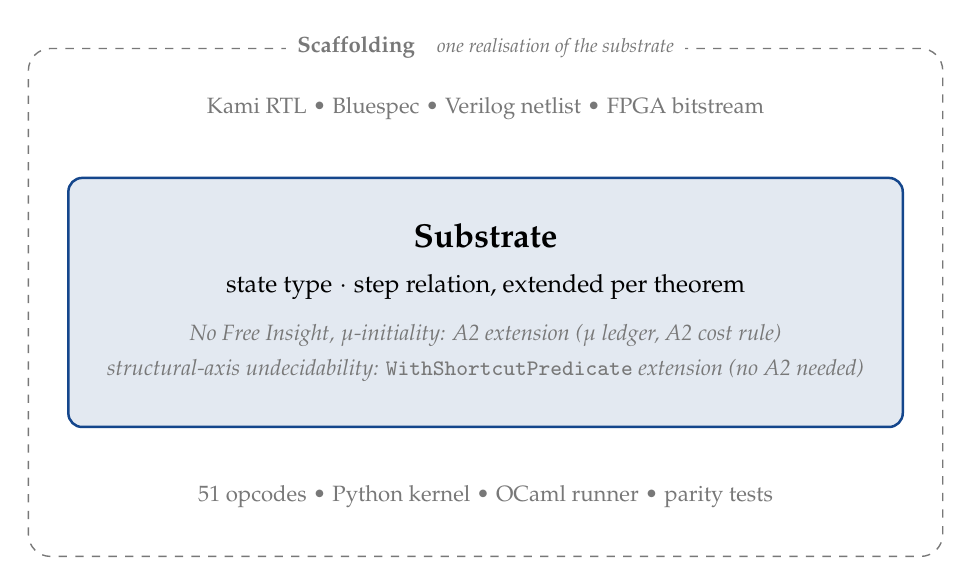
\begin{tikzpicture}[thiele]
% Inner substrate box (drawn first so we can fit the ring around it)
\node[
  draw=thiele@accent, line width=0.9pt,
  rounded corners=5pt,
  fill=thiele@accent!12,
  align=center,
  font=\small,
  inner sep=14pt,
  minimum width=22em,
  minimum height=9em
] (sub) at (0,0) {%
  {\large\bfseries Substrate}\\[0.6em]
  state type\;\textbf{$\cdot$}\;step relation, extended per theorem\\[0.7em]
  {\footnotesize\itshape\color{thiele@gray} No Free Insight, $\mu$-initiality: A2 extension ($\mu$ ledger, A2 cost rule)}\\[0.15em]
  {\footnotesize\itshape\color{thiele@gray} structural-axis undecidability: \code{WithShortcutPredicate} extension (no A2 needed)}
};

% Scaffolding labels above and below (placed outside the inner box but inside the outer ring)
\node[font=\footnotesize, text=thiele@gray, align=center, anchor=south]
  (top-scaff) at ($(sub.north) + (0, 0.6)$)
  {Kami RTL\;\textbullet\;Bluespec\;\textbullet\;Verilog netlist\;\textbullet\;FPGA bitstream};
\node[font=\footnotesize, text=thiele@gray, align=center, anchor=north]
  (bot-scaff) at ($(sub.south) + (0,-0.6)$)
  {51 opcodes\;\textbullet\;Python kernel\;\textbullet\;OCaml runner\;\textbullet\;parity tests};

% Outer scaffolding ring (now fits around substrate + labels)
\begin{scope}[on background layer]
  \node[
    draw=thiele@gray, line width=0.5pt,
    dashed,
    rounded corners=8pt,
    fill=white,
    inner sep=14pt,
    fit=(sub)(top-scaff)(bot-scaff)
  ] (scaff) {};
\end{scope}

% "Scaffolding" label sitting on the outer ring's top edge
\node[font=\footnotesize\bfseries, text=thiele@gray, fill=white, inner xsep=4pt]
  at (scaff.north) {Scaffolding\quad\textnormal{\scriptsize\itshape one realisation of the substrate}};

\end{tikzpicture}
\caption{The substrate-versus-scaffolding distinction. The substrate is the general state-type-and-step-relation layer, extended by different typeclasses for different theorems: No Free Insight needs the certification-floor extension; ledger initiality fixes an initial value and increment schedule, structural-axis undecidability needs the separate \code{WithShortcutPredicate} extension and no A2 at all. Each substrate-level theorem holds for any system carrying the extension it actually uses, regardless of instruction set. The scaffolding is everything that makes this particular substrate runnable, verifiable, and synthesizable. Collapsing the two, or collapsing the two extensions into one, is the most common misread of the document.}
\label{fig:substrate-scaffolding}
\end{figure}

\medskip

\textbf{What ``new model of computation'' means here.}
The model adds an explicit structural and accounting discipline to its execution semantics.
It does not claim additional computable functions.
``Classical shadow'' refers to the selected projection or fragment, not all possible representations on conventional machines.
The law's enforcement, its representation, and its visibility to an observer are separate properties.
It is not a new primitive in the way the Turing machine is.
A Turing machine builds computation out of a tape, a head, and a table.
The substrate takes any state type and any step relation and asks them to obey a law.
So it sits on top of a machine, not beside it, and a Turing machine whose table carries the rule is one of its instances.
What I am claiming is narrower and, to me, more interesting.
The law, the structural state it prices, and what an observer can and cannot see of that state belong in the step.
They are not something a program bolts on afterward.

The renderer experience is the entry point.
I started by trying to build a 3D engine where category-theoretic objects were the runtime objects.
Modules.
Morphisms.
Composition.
Not data structures simulating those things.
The actual things.
The classical CPU saw none of that.
It shuffled bytes that happened to encode the structural state.
Z3 saw formulas that happened to refer to the same shapes.
The structural facts the engine was computing with were in the architecture, not in the data.
That is the concrete shape I had to formalise.
The substrate this document describes is what came out: compositional structure as state, not as an approximation written on top of state.

The formal results give me a precise version of the shadow argument.
\code{thiele\_simulates\_turing} supplies a lift in its file-local transition model.
\code{degenerate\_projection\_theorem} characterizes its selected quotient by an explicit biconditional.
Equal six-field shadows are equivalent to the named equality relation.
Execution preservation additionally requires graph and CSR agreement.
The VM separation witnesses show which structural distinctions its named observations lose.
Recovering every original state from a noninjective projection is impossible.
Choosing defaults is possible, but it does not tell you what the original state contained.

The irrecoverability theorems concern \texttt{vm\_certified}, \texttt{csr\_cert\_addr}, and $\mu$ under their named projections.
Multiple preimages prevent a left inverse recovering every original state.
They do not prevent a section choosing defaults, or an information-preserving encoding with a decoder.

\textbf{What is claimed unique, and what is not.}
A conversational shorthand for this project says there is only one possible substrate.
That shorthand covers three different mathematical claims.
This document does not establish all three.

The first is uniqueness of a law.
Given the A2 cost rule, is there essentially one way to price certification honestly?
Section~\ref{sec:mu} answers a version of this for a fixed schedule.
\code{instruction\_consistent\_measure\_equals\_mu} shows any measure sharing the kernel's own per-instruction schedule and a zero start is forced to equal $\mu$ on every reachable state.
It does not show the schedule itself is forced.
A different schedule prices differently and is a different, equally honest, accounting.

The second is uniqueness of an abstract structural core up to some stated equivalence.
Do all A2-respecting systems collapse, under the right notion of sameness, to one shared mathematical object?
This is the strongest reading of ``only one substrate,'' and it is not a theorem here.
It is a proposal, stated so it can be attacked, not a claim this document proves.
Call a system \emph{adequate} if it carries an A2-respecting certification indicator, a step relation, and an observation interface rich enough to state No Free Insight, ledger initiality, and the diagonal.
The proposed theorem form is
\[
\mathrm{Adequate}(M) \;\Longrightarrow\; \mathrm{StructuralCore}(M) \;\simeq\; \mathrm{ThieleCore},
\]
where $\mathrm{StructuralCore}$ strips a system down to the state, step, and certification data those theorems actually use.
$\simeq$ is an equivalence still to be pinned down.
It is certainly not literal identity of opcodes, storage layout, implementation language, or clock cycles.
None of those enter any premise of any theorem in this document.

The history-retaining target is the test case that shows why $\simeq$ is hard to pin down and why this stays a proposal rather than a theorem.
A target construction discussed later in this document (Section~\ref{sec:projection-nonexistence}; the Coq witness is \code{certification\_agreement\_does\_not\_imply\_descent}) retains the VM's full instruction history, charges the same schedule, and reads certification the same way the VM does.
It agrees with the Thiele VM on every certification and every charge.
It still distinguishes the empty trace from \texttt{JUMP 0 0}, two traces the VM identifies, because it keeps the history and the VM does not.
A2 and certification agreement alone do not force that extra history scaffolding to collapse away.
Any adequacy condition strong enough to make $\mathrm{StructuralCore}$ identify this target with the VM has to say, explicitly, what makes the retained history inessential to the equivalence.
That is exactly the premise the proposal above leaves open.

The third claim is uniqueness of a particular state-transition object, this exact VM state space up to renaming.
That claim is not made anywhere in this document.
It is not what any theorem needs.
The separating witnesses (Section~\ref{sec:categorical}'s graph pair and the irrecoverability theorems above) stand on their own regardless of how the second claim resolves.
They do not require it, and it does not require them.

So the first claim is proved, for a fixed schedule.
The third claim is not made.
The second is the open one, offered here as $\mathrm{Adequate}(M) \Rightarrow \mathrm{StructuralCore}(M) \simeq \mathrm{ThieleCore}$.
It is a conjecture with a stated test case it has to survive, not a theorem this document proves.

\textbf{What this project is not.}
It is not a claim that I solved P vs NP.
It is not a theory of everything.
It is not a claim that computation is physics or that physics is computation.
The CHSH algebraic result is pure math.
The Landauer connection is motivation.
That is the full extent of the physics content here.
The rest is bookkeeping.

%===========================================================================
\section{Things I had to learn first}
\label{sec:vocab}
%===========================================================================

I had been around computers my whole life and paid attention to people like John Carmack on how graphics actually get made, but I came in with none of the formal fields this work turned out to need. By the time the proofs compiled I had needed to learn enough of half a dozen of them that I have to stop here and put down what those fields had words for, before the rest of the document starts using them.

Everything below is what I understood after I went and read about it. If I have anything wrong, tell me. I am not claiming to teach you these subjects. I am putting down what I had to take from each of them to get this work to compile. If you already know one of these subsections, skip it.

\subsection{Bits, bytes, and what a CPU sees}

A bit is one digit that is either zero or one, the smallest fact a machine can hold. Everything else is bits stacked up. Eight of them stacked make a byte, which lands you any number from 0 to 255, and the first thing that genuinely surprised me is that the same byte is also a letter: a convention called ASCII (American Standard Code for Information Interchange) simply agrees to call 65 the letter A, 48 the digit 0, 32 a space. Nothing in the byte knows which it is. The meaning is a convention laid on top of the data, and which convention you read it through is your choice, not the byte's. Hold onto that, because it is the whole argument of this document shrunk down to one byte: the data sits there inert, and everything that matters is in the structure you read it through. I learned the byte part in February.

A word is a chunk of bits the CPU treats as one unit. The kernel math uses 64-bit words (each word can hold any number from 0 to $2^{64} - 1$, about 18 quintillion). The synthesised hardware uses 32-bit words (each word holds 0 to $2^{32} - 1$, about 4 billion). A word is just a sequence of bits with a fixed width. The substrate does not care which width.

A register is a single named storage slot inside the CPU that holds one word. The 51-opcode VM has 16 of them, named r0 through r15. Registers are the fastest place to read or write a value. Memory is a longer list of word-sized slots, accessed by index (the ``address''). The 51-opcode VM has 128 words of memory. That is the entire address space. The substrate has no address space.

The program counter (PC) is one specific register that tracks where in the program the VM is. After every instruction the PC moves forward by one unless the instruction explicitly says jump to a different address.

A stack pointer is a register that points to the top of a region of memory the program uses for nested function calls. CALL pushes a return address there; RET pops it. In the 51-opcode VM, r15 is the stack pointer by convention. The convention is mine. The substrate is not consulted.

A port is a named channel the 51-opcode VM uses to communicate with the outside world. READ\_PORT brings a value in, WRITE\_PORT sends a value out. The kernel does not model the outside world. It just charges $\mu$ for the communication and accepts the value the channel encoding declares. The outside world is welcome to comply. The substrate has no ports.

Modular arithmetic means counting wraps around at a maximum. If the maximum is 16, then 17 wraps to 1 and 19 wraps to 3. ``Modulo 16'' or ``mod 16'' means ``wrap at 16.'' The 51-opcode VM wraps register indices modulo 16 and memory indices modulo 128. If you write r17, the kernel treats that as r1.

Bitwise operations work on the bits of a value rather than treating the value as a number. Bitwise AND of two bits is 1 only when both bits are 1. Bitwise OR is 1 when either is 1. Bitwise XOR (exclusive or, sometimes written $\oplus$) is 1 exactly when the two bits differ. The bitwise version of these does the operation in parallel for every bit position. Bitwise-AND of two 64-bit words gives a 64-bit word. Bit $i$ of the result is the AND of bit $i$ of each input. The bits do not consult each other. The substrate does not see bits.

A shift moves the bits of a value left or right. Left shift by 3 (sometimes written $x \ll 3$) moves every bit three positions to the left, which is the same as multiplying by $2^3 = 8$. Right shift divides by a power of 2. Same idea, opposite direction.

Popcount is the count of 1-bits in a value. Popcount of the byte 11010100 is 4. Sometimes called the Hamming weight; the two names refer to the same thing. Pick one.

Hexadecimal is base 16. Each ``digit'' is one of 0 through 9 or A through F, where A means 10 and F means 15. Hex is convenient for working with bytes because every two hex digits make one byte. Numbers prefixed with 0x are hex: 0xFF is 255, 0xCAFEEACE is the constant unlock key in the Logic Engine accumulator (the Logic Engine is the machine's on-chip formula checker; Section~\ref{sec:entitlement} builds it). It had to be something.

A trap, in the hardware sense, means the machine routes execution to a fixed address instead of advancing normally. It is the hardware equivalent of ``this went wrong, go to the error handler.'' The 51-opcode VM traps LASSERT length mismatches to address 0xF00 (LASSERT is the logic-assertion opcode; Section~\ref{sec:isa} builds it).

An ISA (instruction set architecture) is the list of all instructions the CPU recognises, plus their formats and costs. Each instruction is identified by an opcode (a numeric tag the hardware decodes to choose which behaviour to run). The kernel has 51 opcodes. The substrate has none. The substrate has a step rule.

\subsection{Math notation I will use without explaining it twice}

I read the math symbols out loud the way I learned them, which is whatever the source I was reading suggested they were pronounced as. If you have a different convention in your head, here is what I mean by them.

$\mathbb{N}$ is the natural numbers: 0, 1, 2, 3, and so on. $\mathbb{Z}$ is the integers, which extend the natural numbers with negatives: $\ldots, -2, -1, 0, 1, 2, \ldots$. $\mathbb{R}$ is the real numbers, all the way along the number line including fractions and irrationals like $\pi$ and $\sqrt{2}$.

$\in$ means ``is an element of.'' $x \in S$ reads ``$x$ is in $S$.''

$\subseteq$ means ``is a subset of'' (every element of the left side is also in the right). $\subsetneq$ means strict subset: a subset but not the whole thing.

$\cup$ is set union, the set containing everything in either side. $\setminus$ is set difference: $A \setminus B$ is everything in $A$ that is not in $B$.

$\times$ between two sets is the Cartesian product: $A \times B$ is the set of all $(a, b)$ pairs with $a \in A$ and $b \in B$. Functions from a set $A$ to a set $B$ are written $A \to B$.

For a finite set $S$, $|S|$ means the number of elements in $S$. For a real number $x$, $|x|$ means the absolute value of $x$ (its distance from zero).

$\sum_{i \in T} f(i)$ is the sum of $f(i)$ taken over every $i$ in $T$. The big sigma is the summation symbol.

$\Delta x$ means ``the change in $x$,'' usually the difference between a final and an initial value of $x$.

$\Rightarrow$ is logical implication. $P \Rightarrow Q$ means: if $P$ is true, then $Q$ is true. $\iff$ is the biconditional, also called ``if and only if.'' $P \iff Q$ means both $P \Rightarrow Q$ and $Q \Rightarrow P$.

$\forall$ is ``for every.'' $\exists$ is ``there exists.'' $\forall x.\ P(x)$ reads ``for every $x$, $P(x)$ is true.'' $\exists x.\ P(x)$ reads ``there is some $x$ that makes $P(x)$ true.''

$\langle X \rangle$ around a random variable $X$ means the expected value, the long-run average value of $X$. I picked up this notation reading physics papers about Bell tests.

$\circ$ between two functions is composition: $(f \circ g)(x) = f(g(x))$, first apply $g$, then apply $f$. The same symbol appears in category theory for arrow composition.

$\oplus$ in this document is bitwise XOR. $\otimes$ in this document has exactly one meaning: the MORPH\_TENSOR operator of Section~\ref{sec:isa}, concatenation of two coupling lists into one. Physics writes the same symbol for the tensor product of quantum operators; that sense never appears on these pages, because Section~\ref{sec:chsh} does its quantum work in plain integer arithmetic.

I write $A^T$ for the transpose of a matrix $A$ (rows and columns swapped). $I_n$ is the $n \times n$ identity matrix, which has 1 on the diagonal and 0 everywhere else.

\subsection{Coq, in just enough detail}

Coq is a proof assistant. It is a programming language. The type system is so expressive that you can write proofs as programs and have the compiler check whether they are valid. Section~\ref{sec:coq} has the longer build, including why I trust it. Here is the vocabulary that runs through the rest of the document.

A Theorem in Coq is a named statement followed by a proof. Lemma is the same construct, conventionally used for intermediate results. Definition introduces a named value (a number, a function, a record, anything). Inductive defines a type with a finite list of named constructors, the only ways to build a value of that type. Coq's natural numbers, for example, are an inductive type with two constructors: zero, and ``successor of another natural number.'' Two constructors, infinitely many naturals.

A tactic is a step inside a Coq proof. The tactics that appear in this document include: induction (prove the base case, then prove that if the statement holds at step $n$ it holds at step $n+1$), destruct (split a hypothesis into its cases), exact (provide the literal proof term), reflexivity (prove $x = x$), simpl (simplify the goal by computing), lra (linear real arithmetic; closes goals that are linear inequalities over the reals), nra (nonlinear real arithmetic; handles polynomial inequalities), and psatz (uses Positivstellensatz certificates; it shows a polynomial is non-negative by writing it as a sum of squares). I learned each of them by needing it.

Qed is the keyword that ends a proof. It asks Coq to check the entire chain. If Coq accepts the proof, the theorem is proved.

Admitted is the keyword for ``I am claiming this without proof.'' This is what I am not doing anywhere in the active proof tree. Every Admitted in the kernel would be a bug. Section~\ref{sec:zeroadmit} explains what zero Admitted means. And what it does not.

A Hypothesis (a Coq keyword inside a Section) is a named premise: a statement we accept as given without proof. Hypotheses surface as $\forall$-quantified premises in the conclusion. I use Hypothesis only at named bridge points (the physical-units calibration in Section~\ref{sec:landauer} is the load-bearing example). An Axiom is the global version: a top-level claim accepted without proof. The kernel tier has zero project-local Axiom declarations. The policy is bookkeeping discipline, not faith.

Print Assumptions is the Coq command that lists the global axioms a given theorem ultimately depends on. Running it on the kernel tier shows only standard Coq stdlib axioms (functional extensionality, classical logic for the reals). No project-local axiom appears anywhere in those dependency trees. One thing it does not show: a premise written into the theorem's own statement. Those stay in the type, and ``closed under the global context'' does not make them go away. Whether they hold for the case you care about is something you check by reading the statement.

A total function in Coq always returns a value. Coq requires every function definition to be total. \texttt{vm\_apply} is total. Every state-and-instruction pair has a defined result. Including the error case.

``Parametric in $K$'' means the proof works for any value of $K$. Register, memory, and table sizes are explicit constants in the implementation. Changing them requires rebuilding the affected definitions and checking their representation obligations. A proof about the abstract state alone does not establish that every size choice fits a physical target.

\subsection{Category theory: the part I needed beyond Section~\ref{sec:category}}

Section~\ref{sec:category} builds Category, Object, Morphism, Composition, Identity, and Associativity from scratch. That build is enough for the categorical-separation argument inside this machine. Here is what I had to look up beyond that.

A functor is a structure-preserving map from one category to another. Given two categories $\mathcal{C}$ and $\mathcal{D}$, a functor $F$ from $\mathcal{C}$ to $\mathcal{D}$ sends each object of $\mathcal{C}$ to an object of $\mathcal{D}$. It sends each arrow $f : A \to B$ in $\mathcal{C}$ to an arrow $F(f) : F(A) \to F(B)$ in $\mathcal{D}$. It respects composition ($F(g \circ f) = F(g) \circ F(f)$) and identity ($F(\text{id}_A) = \text{id}_{F(A)}$). Think of a functor as a translation rule between two categorical worlds that keeps the laws intact.

An initial object in a category has exactly one morphism into each object. Here \code{thiele\_trace\_fold\_initial} proves unique evaluation from free instruction lists into a target with a chosen basepoint. It does not prove that the VM state space is initial under certification-preserving state maps. The latter maps may fail to exist; when supplied, their uniqueness on reachable states is a separate theorem.

An embedding is a functor that throws nothing away. That is the whole point of putting the word here: the classical projection of a Thiele state loses things on the way out, and an embedding is the move that does not. Faithful is the precise version of ``loses nothing on arrows'': if two arrows between the same pair of objects in $\mathcal{C}$ land on the same arrow under $F$, they were already the same arrow, so $F$ never quietly fuses two distinct things into one. That is injectivity on each hom-set, checked one pair of objects at a time. Conservative is the version for invertibility: if $F(f)$ has an inverse over in $\mathcal{D}$, then $f$ already had one back in $\mathcal{C}$, so $F$ cannot manufacture an isomorphism that was not there. (An isomorphism is just an arrow with an inverse.) These are different properties, and neither implies the other. The inclusion of the one-object category of the monoid $(\mathbb{N}, +)$ into the one-object category of $(\mathbb{Z}, +)$ is faithful (distinct natural numbers stay distinct integers) but not conservative: $1$ has no inverse in $\mathbb{N}$, yet its image in $\mathbb{Z}$ does. Conversely, the functor from the one-object category of the group $\mathbb{Z}$ to the trivial one-object group is conservative (every arrow in the trivial group is already invertible, so nothing needs reflecting) but not faithful: it fuses every integer onto the same single arrow. Both properties rule out a map inventing structure it should not have, an embedding needs faithfulness specifically, not conservativity, but they rule out different structure and neither substitutes for the other.

A monoidal product is a way of combining two objects, or two arrows, into one. In the category of sets, the Cartesian product $A \times B$ is one. A full monoidal product also comes with a unit and with laws that make the combining behave; that whole bundle is what mathematicians mean by a monoidal structure. MORPH\_TENSOR is tensor-shaped, and I want to be exact about how far that goes. Take two morphisms whose source and target regions don't overlap. Pack them into a single morphism whose coupling is the concatenation. If the regions do overlap, the operation refuses. It also refuses unless the combined regions already exist as modules. Coq checks that local behavior. It does not build the full monoidal category with all its coherence maps. The symbol $\otimes$ below names this operation.

Yoneda's lemma is part of the historical motivation for the early categorical
engine, but it is not used by the formal development and does not occur in any
theorem dependency. The checked results in this document rely on the explicit
category, morphism, and composition structures defined in the repository.

\subsection{Bell-test vocabulary you will meet in Section~\ref{sec:chsh}}

Section~\ref{sec:chsh} builds the CHSH game from scratch. A few foundational terms thread through that section that I will not rebuild each time.

A correlation between two outcomes is the average value of their product. If Alice's outcome $a$ is $\pm 1$ and Bob's outcome $b$ is $\pm 1$, the correlation is $\langle a b \rangle$, which lies between $-1$ and $+1$. A correlation of $+1$ means they always match. $-1$ means they always disagree. $0$ means there is no average correlation. A correlator is one specific correlation in a labelled setting: for example, $E_{00}$ is the correlation when Alice's setting is 0 and Bob's setting is 0.

The marginal of a joint distribution on $(a, b)$ is the distribution on $a$ alone, with $b$ averaged out. Zero-marginal means Alice's marginal gives $\langle a \rangle = 0$ and Bob's gives $\langle b \rangle = 0$. Each outcome is $+1$ or $-1$ equally often, on average. The Section~\ref{sec:chsh} derivation works in this symmetric slice.

A local hidden variable model is a classical-physics-style theory where Alice's and Bob's outcomes are determined by a shared random variable $\lambda$ they agreed on before the game started, plus their own measurement setting. ``Local'' means no communication during the game. ``Hidden'' means $\lambda$ need not be directly observable. ``Variable'' because $\lambda$ is random. Bell's theorem says no local hidden variable model can produce certain correlations that quantum mechanics can.

A no-signaling correlation is one where Alice's marginal does not depend on Bob's setting, and Bob's marginal does not depend on Alice's setting. You cannot learn Bob's setting by looking only at Alice's outputs. Not even in principle. Most correlations we discuss (classical, quantum, and the PR-box below) are no-signaling.

Quantum-realizable, in this document, means ``compatible with some quantum-mechanical state-and-measurement description.'' The NPA framework (Navascu\'es-Pironio-Ac\'in) gives a precise test for this in terms of positive-semidefiniteness of a moment matrix. The test is decidable. Section~\ref{sec:chsh} builds the test.

The PR-box (Popescu-Rohrlich box) is a hypothetical correlation that wins the CHSH game with probability 1, achieving $|S| = 4$. It is no-signaling, but stronger than anything quantum mechanics allows. Nature does not provide it. It is the standard counterexample to the false claim ``any no-signaling correlation is quantum-realizable.''

The Cauchy-Schwarz inequality is the basic inner-product inequality $|\langle x, y \rangle| \leq \|x\| \cdot \|y\|$. It reads: the inner product of two vectors is bounded by the product of their lengths. It is one of the workhorse algebraic moves in the Section~\ref{sec:chsh} derivation.

The Tsirelson bound is the value $2\sqrt{2} \approx 2.828$, the largest CHSH score $|S|$ that any quantum-mechanical strategy can achieve. The classical bound is $2$. The PR-box bound is $4$. Tsirelson sits strictly between classical and PR-box. Nature picked one of these three.

The elliptope, named twice in Section~\ref{sec:claims} and Section~\ref{sec:unknown}, is the formal correlator set represented here by existence of a positive-semidefinite completion. In the standard vector/quantum interpretation it has a physical meaning, but this monograph's Coq development proves the stated real-matrix predicate and its consequences, not a complete physical realization theorem. The zero-marginal fixed-completion slice of that formal set is the part the proof in Section~\ref{sec:chsh} covers.

\subsection{Hardware and synthesis vocabulary}

Section~\ref{sec:hardware} builds the scaffolding stack (Coq kernel, OCaml runner, Kami RTL) carefully. Here is the synthesis-tooling vocabulary that Section~\ref{sec:hardware}'s third subsection uses without expanding each tool.

A hardware description language (HDL) is a programming language for describing circuits. Bluespec SystemVerilog and Verilog are two HDLs. Bluespec is higher-level: you describe rules and the compiler figures out the gate-level details. Verilog is lower-level: you describe gates and wires more directly. Verilog RTL specifically means ``register-transfer level'' Verilog, which describes how data moves between registers each clock cycle. It is what synthesis tools consume. They do not eat Bluespec.

Synthesis is the process of compiling a hardware description down to actual logic gates (the building blocks of chips). yosys is an open-source synthesis tool. After synthesis, place-and-route assigns the gates to physical positions on a chip and connects them. nextpnr-xilinx is the place-and-route tool for the Xilinx FPGAs this design targets. The last stretch is producing a bitstream, the binary file the FPGA reads to configure itself, and prjxray does it in two moves: fasm2frames packs the routed design into configuration frames, then xc7frames2bit writes the frames out as the bitstream. Four steps, four tools, one chip.

An FPGA (field-programmable gate array) is a chip you can program after manufacturing. The gates are physical. The connections between them are configurable. An ASIC (application-specific integrated circuit) is the non-programmable version: gates fixed at manufacturing time for one specific design.

A LUT (look-up table) is the basic logic primitive in an FPGA: a small memory that maps a fixed-length list of inputs to an output, programmed at configuration time to implement any small boolean function. A flip-flop is a one-bit memory cell that holds its value across clock cycles. A carry chain is specialised wiring for fast addition. Distributed RAM is RAM built from LUTs. Block RAM is dedicated RAM blocks on the chip. DSP slices are specialised hardware for digital-signal-processing arithmetic. The synthesised K325T design uses 0 DSP slices because yosys is invoked with \texttt{-nodsp}, mapping the wide multiplier in the multi-cycle witness checker (Section~\ref{sec:hardware}) to LUTs instead. The substrate would also accept a DSP-inferred mapping. The choice is a chip-capacity and place-and-route runtime trade-off, not a correctness one.

A JSON netlist is the gate-level circuit serialised in a JSON text file (JSON is a standard text format for structured data). A VCD waveform is a Value Change Dump, a record of every signal's value at every time step in a simulation. The name describes the file. iverilog is an open-source Verilog simulator. It runs the design and produces a VCD output you can inspect.

A bisimulation is a precise notion of ``two systems behave the same.'' You pick a relation between the states of one system and the states of the other. Related states have to agree on whatever you chose to observe, and whenever one of them takes a step, the other has a matching step that lands in related states again. That is looser than ``same output state, field by field.'' Field-by-field equality is one particular, stronger contract. Section~\ref{sec:hardware} says exactly which observations and transitions the hardware relation covers. A parity test is the empirical cousin: run two implementations on the same battery of inputs and check they agree, a correspondence earned by testing rather than by proof. The kernel-to-OCaml boundary is closed that way, and the document says so where it happens.

\subsection{Other terms I use without rebuilding}

Provenance, in software, means the recorded chain of where an object came from. A morphism's provenance is the specific sequence of MORPH and COMPOSE instructions that built it. You can replay the chain.

Simulation, in computer science, means one system imitating another's input-output behaviour. A Turing machine simulates a Thiele Machine when it produces the same outputs on the same inputs, by writing the whole Thiele state out across its tape and grinding through it. That is real, and it matters, and it is exactly the thing people reach for when they want to wave the whole question away: if a tape can stand in for the state, what was the difference? The difference is that the tape carries a picture of the state, not the state, the way a photograph of a fire keeps you exactly as warm as any other photograph. The cost ledger and the A2 rule live in the step relation, not in the bytes, and an encoding copies the bytes. Simulating the substrate is not being the substrate. A Turing machine can be one, though: build its transition table so the rule is its own step rule, and it is an instance, not a simulation. What no machine can do is make a simulated rule binding just by writing it down on tape.

Projection, in mathematics, is a function that drops information on purpose. The classical projection of a Thiele state is the one that does the dropping I keep pointing at: it throws away $\mu$, certification, and the morphism graph, and keeps registers, memory, and the program counter. That is the exact list. The three it keeps are the three a Turing machine already has, which is the whole reason the projection lands you back in ordinary computation. The three it drops are the three that were doing the new work. Nothing about the projection is wrong; it is a perfectly good function. It just costs you everything that made the state more than a tape.

Quotient, in mathematics, is the operation of declaring two things the same when they agree on what you decided to look at, and then working with the lumped-together classes instead of the originals. The classical projection is exactly that kind of move: any two Thiele states that match on registers, memory, and the program counter get swept into the same class, even when their $\mu$, their certification, and their morphism graph were completely different. So the projection is not just dropping fields one at a time; it is gluing together states that the dropped fields kept apart. That is the precise sense in which it loses information, and it is comforting that the math already had the word sitting there waiting.

A kernel of a map is context-dependent. For a group or module homomorphism it is the inverse image of the identity element; for the quotient induced by a projection $\pi$, the relevant equivalence relation is $s \sim t$ exactly when $\pi(s)=\pi(t)$. The classical projection in this document uses that second quotient reading. ``Kernel'' wears three different hats in this document and I would rather call that out than let it ambush you: this mathematical usage; the Coq proof core, meaning the kernel-tier theorems in Section~\ref{sec:claims}, which is scaffolding I lean on, not the substrate itself; and the operating-system kernel, which I imply at most by analogy and never actually use. Whenever the word shows up, the surrounding sentence tells you which one is meant.

Embedding is a function that preserves structure and is injective. Faithful embedding additionally preserves all the structure-relevant distinctions.

An injection is a function where no two inputs map to the same output. A surjection is a function whose image covers every possible output. Their negations are noninjective and nonsurjective.

Decidable, in computer science, means there is an algorithm that always halts with a yes-or-no answer. Keep the question and the algorithm apart. The predicate is the mathematical claim $P(x)$. The decision procedure is the algorithm, and it only decides $P$ once there is a proof that its answer matches. The integer-only Z-arithmetic check in CHSH\_LASSERT always halts with a Boolean. Its soundness theorem says a pass means the stated real-matrix predicate holds.

Polynomial complexity: an algorithm is polynomial-time if there is some power $k$ such that the algorithm's running time on inputs of size $n$ is at most a constant times $n^k$. Polynomial-space is the analogous concept for memory used. The class P is decision problems solvable in polynomial time. The class NP is decision problems where, given a candidate solution, a polynomial-time algorithm can check whether the solution is correct. The famous P-vs-NP question asks whether finding is fundamentally harder than checking. Nobody has proved either direction. Section~\ref{sec:unknown} discusses why my \code{mu\_budget\_decidable} / \code{mu\_budget\_verifiable} predicates are not a P-vs-NP result.

Determinant: a number computed from a square matrix that says whether the matrix is singular (zero determinant means the matrix collapses some direction to zero). For a $2 \times 2$ matrix $\begin{pmatrix} a & b \\ c & d \end{pmatrix}$ the determinant is $ad - bc$. For larger matrices, you can compute it by ``expansion along a row'': pick a row, for each entry take the determinant of the submatrix you get by deleting that entry's row and column (with alternating signs), multiply by the entry, and sum. The recursion bottoms out at the $2 \times 2$ case above. Section~\ref{sec:chsh} walks the explicit calculations for the $3 \times 3$ cases I need.

Schur complement: a way of turning a question about a block matrix into a question about a smaller matrix. If $\begin{pmatrix} A & B \\ C & D \end{pmatrix}$ is a block matrix where $A$ is invertible, the Schur complement of $A$ is $D - C A^{-1} B$. The fact I use: for a symmetric real block matrix whose pivot $A$ is positive definite, the whole matrix is positive-semidefinite exactly when the Schur complement is. Invertible alone is not enough. The pivot has to be positive definite. The Section~\ref{sec:chsh} build uses this for the $4 \times 4$ block of the specified moment matrix.

A principal submatrix is the square subblock you get by picking a subset of indices and keeping only the rows and columns at those indices. A standard result is that a matrix is positive-semidefinite if and only if every principal submatrix is positive-semidefinite. Every one. Section~\ref{sec:chsh} relies on this.

\subsection{The axioms (A1 through A6)}
\label{sec:axioms}

The Thiele Machine has a small numbered list of substrate-level axioms. They appear by name (``A2,'' ``A3,'' \ldots) throughout the document and the formalization. The list below is what each name means, where it lives in the kernel, and what its conclusion is. The axioms are substrate-level; the kernel is scaffolding-level; the list bridges the two.

The kernel keeps two parallel axiom-numbering systems because two parallel substrate abstractions are formalised. The \code{AbstractCertMachine} record carries A1 (the cert indicator exists, by record existence) and A3 (only cert-setters flip it, the \texttt{acm\_preserve} field). A2 (cert starts unset) and A4 (cert-setters cost $\geq 1$) live alongside the record, not in it: A2 is the \texttt{acm\_cert M s0 = false} hypothesis to \texttt{abstract\_nfi}, A4 is the standalone lemma \code{cert\_addr\_setter\_cost\_pos}. The consolidated \code{CertificationSystem} record folds the cost-on-certification semantic content into a single field kept by the name A2 (the load-bearing piece). The \code{QuantitativeCertificationSystem} extension adds A3--A6, which lift the cost-floor result from $\geq 1$ to $\geq K$ for an arbitrary threshold $K$. The two numbering systems agree on the cost-on-certification semantic content; they disagree on which axiom carries that content (A4 in the AbstractCertMachine list, A2 in the consolidated CertificationSystem list). When the rest of this document says ``A2,'' it means the cost-on-certification rule, in the consolidated CertificationSystem sense.

\begin{description}[style=nextline,leftmargin=0pt,itemindent=0pt,labelsep=0.5em,font=\bfseries]
\item[A1 (state includes a certification indicator).] An \code{AbstractCertMachine} record bundles a state type \texttt{S}, a step function \texttt{acm\_step}, and a boolean cert indicator \texttt{acm\_cert : S $\to$ bool}. A1 is the structural requirement that this indicator exists at all. In Coq, A1 is enforced by the record type itself. There is no way to hand Coq an \code{AbstractCertMachine} value with \texttt{acm\_cert} left blank; it reads the field as missing and declines to build the record, the way a clerk declines a form with an empty box. A1 is discharged at type-check time.

\item[A2 (cost-on-certification).] In the consolidated \code{CertificationSystem} record, Coq field \texttt{cs\_cert\_costs}. Statement: for every state $s$ and instruction $i$, if \texttt{cs\_cert s = false} and \texttt{cs\_cert (cs\_step s i) = true}, then \texttt{cs\_cost i $\geq$ 1}. In words: any single step that flips the certification predicate from no to yes must have positive cost. This is the load-bearing axiom for No Free Insight. \code{universal\_nfi\_any\_substrate} concludes from A2 alone that every trace from uncertified to certified has total cost $\geq 1$. Note: in the AbstractCertMachine numbering, the same content appears as A4 (cert-setters cost $\geq 1$). The AbstractCertMachine A2 is the separate precondition that the cert indicator starts unset, which the consolidated system handles as a theorem hypothesis instead of a numbered axiom.

\item[A3 (cost bounds witness growth).] Coq field \code{qcs\_cost\_bounds\_witness} on the record \code{QuantitativeCertificationSystem}. Statement: for every state $s$ and instruction $i$, \texttt{qcs\_witness s + cs\_cost i $\geq$ qcs\_witness (cs\_step s i)}. In words: each instruction's cost is an upper bound on how much the system's accumulated evidence (the ``witness'') can grow in that step. The cost is the speed-limit on evidence accumulation. (In the AbstractCertMachine numbering, A3 is the field \texttt{acm\_preserve}: non-cert-setter instructions preserve the cert indicator. The two A3s are distinct properties on distinct record types; the monograph's A3 is the quantitative one above.)

\item[A4 (witness nondecreasing).] Coq field \code{qcsf\_witness\_nondecreasing} on the record \code{QuantitativeCertificationSystem\_full}. Statement: for every $s$ and $i$, \texttt{qcs\_witness s $\leq$ qcs\_witness (cs\_step s i)}. A3 and A4 point in opposite directions: A3 caps how fast the witness can grow ($w' \leq w + \text{cost}$), A4 stops it from shrinking ($w \leq w'$). Neither implies the other. $(w, \text{cost}, w') = (1, 0, 0)$ satisfies A3 with non-negative cost yet violates A4, and $(0, 0, 1)$ does the reverse, so A4 is its own field, not a consequence of A3. It is also idle: the $\geq K$ floor telescopes through A3, A5, and A6 alone and never touches A4. The field is kept so downstream consumers that want witness monotonicity in hand have it without re-deriving it; the consolidated \code{QuantitativeCertificationSystem} record drops A4 entirely, carrying only A3 and A5.

\item[A5 (certification requires witness).] Coq field \code{qcs\_cert\_threshold\_witness} on \code{QuantitativeCertificationSystem}. Statement: \texttt{cs\_cert s = true $\to$ qcs\_witness s $\geq$ qcs\_threshold}. In words: certification cannot fire until the system has accumulated at least \texttt{qcs\_threshold}-worth of evidence. This is what lets the quantitative theorem push the cost floor from $\geq 1$ to $\geq K$, where $K$ is the threshold. Pay more, certify more.

\item[A6 (witness initial zero).] The hypothesis that the run starts with zero witness, stated as a precondition on the quantitative theorem rather than a record field. Without A6 the telescoping bound becomes $K - \texttt{initial witness}$ instead of $K$. Zero is a clean place to start.
\end{description}

A1 through A6, as the consolidated records state them, are independent of any specific instruction set; the AbstractCertMachine variant is the one exception, typing its step over the VM's own instruction type. They are conditions on Coq record types; supplying instances of those record types is the only way to invoke the corresponding theorems. The 51-opcode VM supplies them by construction: the kernel builds two concrete \code{CertificationSystem} values for the VM (one for the \texttt{csr\_cert\_addr} channel, one for the \texttt{vm\_certified} channel), each discharging A2 from the existing \code{no\_free\_certification} kernel theorems. A separate substrate-level abstraction (the \texttt{Substrate} typeclass) carries a related but distinct field \texttt{mu\_monotone} stating that the cost ledger never decreases on a step. \texttt{mu\_monotone} is a strictly weaker general-purpose monotonicity property than A2: A2 specifically asserts the cert transition costs $\geq 1$, whereas \texttt{mu\_monotone} only asserts the ledger does not go down. The two coincide on the 51-opcode VM, where every instruction adds non-negative cost and the cert transition adds at least 1. Two locks on the same door, by different keys.

That is the vocabulary. From here on, the document uses these words without rebuilding them. Section~\ref{sec:formal} is where the formal machine state begins; experts should jump there. Everyone else stays for the walk.

%===========================================================================
\section{The structural axis: the projection classical models drop}
\label{sec:turing}
%===========================================================================

\noindent\textbf{Why this section exists.} This section exists because a renderer I was building in January 2025 walked me into a wall, and the wall turned out not to be made of what I thought.

The renderer was a categorical engine. I had built it so the things running at runtime were the category-theory objects themselves: modules were objects, transformations between them were morphisms, composing two transformations was literally composition, and running two independent parts side by side was the monoidal product (Section~\ref{sec:vocab} builds all of these). I was not simulating category theory on top of ordinary data. The structure was the thing the engine ran on. And it worked, which is the part I still find a little funny: within weeks the same engine that was supposed to draw pixels was running physics on the identical primitives, and I had not planned that and did not at first believe it.

Then I tried to prove something about what it was doing, and the floor went out. The machine underneath, the ordinary CPU, had seen none of the structure the entire time. (That ordinary architecture, one processor and the memory passing data back and forth across a single bus, is the von Neumann machine, after John von Neumann who wrote it down in 1945; every laptop and phone and server you have ever touched is one.) It had been faithfully shuffling the bytes my modules and morphisms happened to be spelled out in, faithful the way a printing press is faithful to a poem it cannot read. When I brought in Z3 to verify the morphism chains the engine was reasoning with, I met the same blindness in different clothes: Z3 saw formulas, true ones, that happened to refer to the shapes, and it never once saw a shape. For a long stretch I took this for a Z3 problem, a tooling problem, the kind you solve by getting cleverer with the solver. It was not a Z3 problem. The structure I wanted checked was real and was carrying the whole computation, and there was nowhere in the machine for it to sit as a thing the machine itself had to answer for. I was asking a tool to certify a fact about the one part of the computation the computation had no place to keep. You do not get cleverer your way into a slot that was never built.

The Thiele Machine is that slot. It is the substrate the engine had needed all along and could never be handed on the hardware it was running on: a machine where the structure is first-class state instead of a pattern in the bytes, where composing that structure is a step the machine takes rather than something you read back out afterward, and where committing to a structural fact is an act the machine is charged for and cannot quietly perform for free. Everything past this point is that substrate's correctness conditions, laid out in English you can follow and check yourself, with a Coq proof standing next to each one. The Coq is not what makes any of it true. It is there because my own eye slides straight over the gaps in an argument I am hoping is right, and I wanted a reader that would not let me. This section is the long-form answer to a question a stuck renderer put to me and would not drop until I quit trying to out-clever it and went looking for what was actually missing.

A2 is expressed in the transition interface, as the proof field \texttt{cs\_cert\_costs}. Within the VM, it is established from the instruction semantics. Observers that discard the relevant fields cannot reconstruct them from the remainder. The irredundancy result is relative to those projections, not a requirement for separately named fields in every implementation.

The law is meaningful beyond this ISA: the abstract state type and predicate are parameters. This supports studying many instances. It does not establish that all observable changes have positive cost or that arbitrary predicates are independent geometric dimensions.

\subsection{Substrate-independence: the abstract setup}

The kernel theorem \code{universal\_nfi\_any\_substrate} is written to be as hard to wriggle out of as I knew how to make it, and the way you make a theorem hard to wriggle out of is to make it ask for almost nothing. It takes any abstract computational system at all, and by any I mean it genuinely does not care what the system is made of or whether it looks anything like the machine in this document. It asks for five pieces and refuses to ask for a sixth. A set of states, and a state can be whatever it is for you: bits on a tape, words in a register file, cells in memory, it makes no difference to the theorem. A set of instructions, the moves the thing can make. A step rule, which takes a state and an instruction and hands back the next state. A cost function, which pins a non-negative integer to each instruction. And a certification predicate, a plain yes-or-no on states that says whether a given state counts as certified. That is the entire list. The reason I keep leaning on how short it is: any objection that begins ``sure, but that only holds for your particular machine'' has nothing to attach to once the result has agreed to run on something this bare.

One premise, labelled A2 and named \texttt{cs\_cert\_costs} in the kernel: if any single step flips the certification predicate from no to yes, the instruction that did it cost at least 1. One conclusion: every trace that starts uncertified and ends certified has total cost at least 1.

And it does not care how powerful the thing is, in either direction. It never asks whether your system can compute everything a Turing machine can (the word for that is Turing-complete: you are Turing-complete if you can simulate a Turing machine, at most Turing-equivalent if a Turing machine can simulate you). It never asks for the reverse either. Stronger than a Turing machine, weaker, dead even, none of it reaches the floor. Bring the five pieces, charge A2 on the flip, and you are in scope. The floor does not check your computational class at the door, because it was never about what you can compute. It is about what your step is allowed to do for free.

The categorical-separation result in Section~\ref{sec:categorical} concerns the specified observable tuple. Two states may agree there and differ in their graph. A full conventional encoding could preserve the graph; a decoder could then inspect it. The theorem identifies what this observation discards.

The abstract theorem requires a designated predicate and the A2 cost premise. An arbitrary Turing-machine trace is not an instance merely because it is a computation. It becomes an instance when the required state interpretation, step function, cost, and proof are supplied.

\begin{figure}[!htbp]
\centering
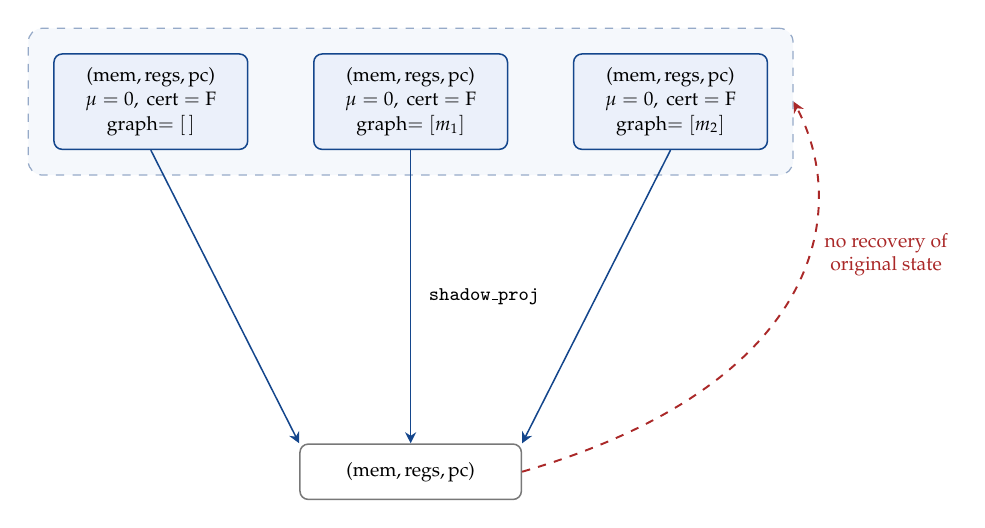
\begin{tikzpicture}[thiele]
\tikzset{
  bigtnode/.style={
    draw=thiele@accent, line width=0.55pt,
    rounded corners=3pt,
    inner sep=5pt,
    fill=thiele@pale,
    font=\scriptsize,
    align=center,
    minimum width=7em,
    minimum height=3.2em
  },
  bigcnode/.style={
    draw=thiele@gray, line width=0.55pt,
    rounded corners=3pt,
    inner sep=6pt,
    fill=white,
    font=\scriptsize,
    align=center,
    minimum width=8em,
    minimum height=2.0em
  }
}
% Thiele layer (top): three states whose classical fields agree
\node[bigtnode] (T1) at (-3.3, 2.3)
  {(mem,\,regs,\,pc)\\[0.1em]$\mu=0,~\text{cert}=\text{F}$\\[0.1em]graph$=[\,]$};
\node[bigtnode] (T2) at (0, 2.3)
  {(mem,\,regs,\,pc)\\[0.1em]$\mu=0,~\text{cert}=\text{F}$\\[0.1em]graph$=[m_1]$};
\node[bigtnode] (T3) at (3.3, 2.3)
  {(mem,\,regs,\,pc)\\[0.1em]$\mu=0,~\text{cert}=\text{F}$\\[0.1em]graph$=[m_2]$};

% Background "fiber" group on Thiele side
\begin{scope}[on background layer]
  \node[draw=thiele@soft, dashed, line width=0.45pt, rounded corners=5pt,
        inner sep=9pt, fill=thiele@pale!50, fit=(T1)(T2)(T3)] (fiber) {};
\end{scope}

% Classical state (bottom)
\node[bigcnode] (C) at (0, -2.4) {(mem,\,regs,\,pc)};

% Three canonical projections down
\draw[proj] (T1.south) -- (C.north west);
\draw[proj] (T2.south) --
  node[right=3pt, font=\scriptsize\ttfamily] {shadow\_proj} (C.north);
\draw[proj] (T3.south) -- (C.north east);

% Non-existent lift, drawn as one red dashed curve up to the fiber group
\draw[nolift] (C.east) .. controls (5.2,-1.3) and (5.6, 0.9) ..
  node[right=2pt, font=\scriptsize, text=thiele@red, align=center, pos=0.6]
       {no recovery of\\original state} (fiber.east);

\end{tikzpicture}
\caption{Selected projections identify richer states. Multiple preimages rule out recovering every original state from its projection. A section choosing default metadata remains possible; it does not recover the omitted original data. The diagram suppresses some retained fields for legibility.}
\label{fig:projection}
\end{figure}

\subsection{What is canonical, and under which conditions}

Three results should be kept separate. \code{universal\_nfi\_any\_substrate} proves a floor for every system satisfying A2. \code{mu\_is\_initial\_monotone} proves ledger uniqueness on reachable states given the initial value and exact instruction increments. The projection theorems identify information lost by specific observations.

The abstract \code{CertificationSystem} carries an arbitrary state type, instruction type, step function, nonnegative instruction cost, Boolean predicate, and proof of A2. Its state need not have separate cost and certification fields. A conventional encoding may carry both. The classification is about the supplied semantics, not the physical names or layout of registers.

A fixed machine can enforce an invariant through its prescribed transitions. A simulator preserves that invariant when its correctness contract establishes the correspondence. A defective simulator does not establish that every simulator or every conventional machine lacks enforcement. Equally, a protected internal law does not automatically authenticate a transcript presented by an external party.

Certification is one instance of this framework. A proposed family of observables $\alpha_i:S\to X_i$ needs explicit events and cost laws for each claimed guarantee. Merely collecting predicates supplies neither a topology nor a metric, nor independence among the observations. The present ISA permits zero-cost changes even to partition structure.

\subsection{The canonical contrast: the Turing machine}

Here is what I had to learn about Turing machines to compare what I built to one. I went and read about them on my own. I'm walking through it because I had to walk through it. If I have anything wrong below, I'm relaying what I read, so tell me.

What I read says Alan Turing described his machine in 1936 to make precise the intuitive notion of ``algorithm.'' The machine, as I understand it, is this:

\begin{itemize}
\item An infinite tape. Think of it as an infinitely long strip of paper, divided into cells. Each cell holds one symbol from a finite alphabet, say $\{0, 1, \texttt{blank}\}$.
\item A read/write head. One cell at a time. It reads the symbol, overwrites it if the table says to, then moves left or right.
\item A finite set of states, $Q = \{q_0, q_1, \ldots, q_n\}$. The machine is in exactly one state at a time. $q_0$ starts the run. Some states halt it.
\item A transition table. Given the current state and the symbol under the head, it says: write this, move left or right, enter that state.
\end{itemize}

That is the entire machine. Nothing else.

Here is what I read as the remarkable thing about this simple machine: it can compute \emph{anything that can be computed by following a definite procedure}. The sources I dug up claim every algorithm that has ever been written, in every programming language that has ever existed, can be translated into a Turing machine. The label I found for this is the Church-Turing thesis. The original claim (Church 1936, Turing 1936), as I read it, is specifically about \emph{effective calculability}: anything that can be computed by following a mechanical, finite, step-by-step procedure, a Turing machine can also compute. I did not find a counterexample. I also have not verified the thesis myself. I am reporting the ground I had to stand on before I could push against it.

The claim about physical hardware is a related but separate conjecture, called in the sources I read the \emph{physical Church-Turing thesis}: every physical computing device is computationally equivalent to a Turing machine. As I read it, this is an empirical claim about physics, not proven mathematics. I did not find a built physical counterexample. Your laptop, your phone, every server in every data center: in the usual computability sense, they compute no more functions than a Turing machine computes. The differences I found are resource differences. Speed. Space. Energy. Cost. The class of computable functions stays the same.

\subsection{The observation boundary}

A Turing-machine transition reads a local symbol and control state; a computation can nevertheless derive global properties or retain prior evidence in its state. The relevant impossibility here concerns a particular projection: when two full states have equal observations and different structural properties, no function of that observation recovers the differing property universally.

A structural opcode can expose or check a property through the richer state. Its guarantee must be read from its semantics. An accumulated ledger alone records a total; locating an event in history requires the trace as well. A positive payment alone does not establish semantic truth.

\subsection{Structural cost and other resource measures}

This framework tracks its own event-sensitive cost schedule alongside ordinary execution. It does not claim that complexity theory studies only two resources or cannot model verification costs. The intended contribution is the particular composition of transition laws, structural state, observation interfaces, and accounting results, with the conditions stated in each theorem.

\subsection{The subsumption theorems, in full}

Section~1 framed classical computation as the degenerate fragment of the Thiele substrate, the corner where the structural axis lies dormant and nothing ever lights it up. That framing is four theorems in the kernel, and I am setting their statements and proof sketches down below in plain math, so you can hold the framing up against the proofs and decide for yourself, without taking my word for either one and without leaving this page to do it.

\begin{theorem}[D2 faithfulness]
For every classical program $\mathrm{prog}$ (a sequence of \texttt{vm\_instruction} values each satisfying \code{is\_classical\_opcode}) and every starting state $s_0$, let $s_n$ be the state after running $\mathrm{prog}$ on $s_0$. Then (a) $\texttt{shadow\_proj}(s_n)$ extracts exactly the six projected fields of $s_n$ (\texttt{vm\_regs}, \texttt{vm\_mem}, \texttt{vm\_pc}, \texttt{vm\_mu}, \texttt{vm\_err}, \texttt{vm\_certified}); and (b) the structural layer is preserved: $s_n.\texttt{vm\_graph} = s_0.\texttt{vm\_graph}$, $s_n.\texttt{vm\_csrs}.\texttt{csr\_cert\_addr} = s_0.\texttt{vm\_csrs}.\texttt{csr\_cert\_addr}$, and $s_n.\texttt{vm\_certified} = s_0.\texttt{vm\_certified}$.
\end{theorem}

\begin{proof}
Part (a) unfolds \texttt{shadow\_proj}: by definition it extracts exactly those six fields, and reflexivity closes it. Part (b) is D3 conservativity (next theorem) iterated over the program. \qed
\end{proof}

\begin{plainreading}
Classical programs leave the structural axis alone. The shadow you see equals the full state's projected fields. The graph and cert channels stay at whatever they were at the start.
\end{plainreading}

\begin{theorem}[D3 conservativity]
If $\code{is\_classical\_opcode}(i) = \mathrm{true}$ and $s' = \texttt{vm\_apply}(s, i)$, then $s'.\texttt{vm\_graph} = s.\texttt{vm\_graph}$, $s'.\texttt{vm\_csrs}.\texttt{csr\_cert\_addr} = s.\texttt{vm\_csrs}.\texttt{csr\_cert\_addr}$, and $s'.\texttt{vm\_certified} = s.\texttt{vm\_certified}$. By induction over the program list, classical programs preserve all three.
\end{theorem}

\begin{proof}
Case analysis on the instruction $i$. The predicate \code{is\_classical\_opcode}$(i) = \mathrm{true}$ holds exactly for the compute, memory, control-flow, ordinary I/O, heap, and \texttt{MORPH\_GET} / \texttt{TENSOR\_GET} opcodes: the ones whose \texttt{vm\_apply} rule mutates only \texttt{vm\_regs}, \texttt{vm\_mem}, \texttt{vm\_pc}, \texttt{vm\_err}, \texttt{vm\_mu}, \texttt{vm\_logic\_acc}, \texttt{vm\_mu\_tensor}, or \texttt{vm\_mstatus}. Twenty-two opcodes return \texttt{false} from \code{is\_classical\_opcode} and are excluded by the premise, but not all for the same reason. \texttt{PNEW}, \texttt{PSPLIT}, \texttt{PMERGE}, \texttt{TENSOR\_SET}, \texttt{MORPH}, \texttt{COMPOSE}, \texttt{MORPH\_ID}, \texttt{MORPH\_DELETE}, and \texttt{MORPH\_TENSOR} mutate graph or module-tensor state. \texttt{MORPH\_ASSERT} can write the cert-address channel on success; \texttt{CERTIFY} writes the top-level certification flag; \texttt{CHSH\_TRIAL} mutates the witness counters. \texttt{LASSERT}, \texttt{LJOIN}, \texttt{EMIT}, \texttt{REVEAL}, \texttt{PDISCOVER}, \texttt{CHSH\_LASSERT}, and the four Q\textsubscript{1+AB} \texttt{CHSH\_LASSERT} variants are also outside the classical fragment because they carry validation, revelation, discovery, tensor-charge, or mandatory-floor semantics. The D3 proof only needs the forward direction: for each opcode that \code{is\_classical\_opcode} admits, direct inspection of the apply rule leaves \texttt{vm\_graph}, \texttt{csr\_cert\_addr}, and \texttt{vm\_certified} fixed. Iterating over the program list by induction closes the trace-level preservation. \qed
\end{proof}

\begin{plainreading}
The classical opcodes are defined by what they don't touch. They may change the projected working fields, including the ledger charge assigned to the instruction, but they leave the graph and certification channels alone. A program built only out of them cannot disturb those channels, even if you wanted it to. That dormancy is by construction, not by accident.
\end{plainreading}

\begin{theorem}[Thiele simulates Turing]
Lift a Turing configuration by keeping the TM part and setting $\mu$ to zero: $\texttt{lift\_config}(c) := \{\, \texttt{th\_tm\_config} = c;\ \texttt{th\_mu} = 0\,\}$. Then for every fuel $n \in \mathbb{N}$, transition table $\delta$, and TM configuration $c$:
\[
(\texttt{thiele\_run}\ n\ \delta\ (\texttt{lift\_config}\ c)).\texttt{th\_tm\_config} \;=\; \texttt{tm\_run}\ n\ \delta\ c.
\]
\end{theorem}

\begin{proof}
Induction on the fuel $n$.

\emph{Base ($n = 0$).} Both \texttt{thiele\_run}\,0 and \texttt{tm\_run}\,0 return their inputs unchanged. Reflexivity.

\emph{Step ($n+1$).} Unfold one step on both sides. Let $c' = \texttt{tm\_step}\ \delta\ c$ when defined. On a lifted configuration, \texttt{thiele\_step}'s TM portion is exactly $\texttt{tm\_step}\ \delta\ c$: structural fields are not consulted, and lifted $\mu$ stays at $0$ because TM steps are classical. Apply the induction hypothesis to the next $n$ steps from $\texttt{lift\_config}(c')$. \qed
\end{proof}

\begin{plainreading}
Take any Turing-machine configuration and drop it into the Thiele substrate untouched: the TM part stays exactly as it was, $\mu = 0$, the structural fields empty. Now run \texttt{thiele\_run} on it. Nothing happens that wasn't going to happen anyway. Step for step the TM portion does precisely what the standalone machine would have done, and because every move it makes is a classical move, the ledger never comes off zero. The induction on fuel just carries that out to the whole trace. The Turing machine is sitting inside the larger object running its same computation on its same tape to its same answer, having paid nothing, and from where it stands there is no way to tell it has been subsumed at all. That is what subsumption is supposed to look like: the old thing keeps working, identically, for free.
\end{plainreading}

\begin{theorem}[Degenerate projection theorem (four-part)]
The following four propositions hold simultaneously:
\begin{enumerate}
\item \emph{Faithful embedding.} For every fuel $n$, transition table $\delta$, and TM configuration $c$:
\[
(\texttt{thiele\_run}\ n\ \delta\ (\texttt{lift\_config}\ c)).\texttt{th\_tm\_config} \;=\; \texttt{tm\_run}\ n\ \delta\ c.
\]
\item \emph{\texttt{shadow\_proj} is the quotient map.} For all Thiele states $s_1, s_2$:
\begin{multline*}
\texttt{shadow\_proj}(s_1) = \texttt{shadow\_proj}(s_2) \\
{} \Longleftrightarrow\; \code{eq\_on\_classical\_shadow}(s_1, s_2).
\end{multline*}
\item \emph{Classical traces respect the compatibility relation.} For every classical program $\mathrm{prog}$ and every two Thiele states $s_1, s_2$ with $\texttt{shadow\_proj}(s_1) = \texttt{shadow\_proj}(s_2)$ \emph{and} $s_1.\texttt{vm\_graph} = s_2.\texttt{vm\_graph}$ \emph{and} $s_1.\texttt{vm\_csrs} = s_2.\texttt{vm\_csrs}$:
\[
\texttt{shadow\_proj}(\texttt{run}(\mathrm{prog}, s_1)) \;=\; \texttt{shadow\_proj}(\texttt{run}(\mathrm{prog}, s_2)).
\]
Shadow agreement alone is not a strong enough hypothesis. \texttt{TENSOR\_GET} and \texttt{MORPH\_GET}, both classical opcodes, read \texttt{vm\_graph} into a visible register; \texttt{HEAP\_LOAD} and \texttt{HEAP\_STORE} read \texttt{csr\_heap\_base} out of \texttt{vm\_csrs}. Two states can agree on all six projected fields and still disagree on the graph or the heap base, and either instruction then writes a different value into a projected register, breaking the shadow-only version of this claim. The extra agreement on \texttt{vm\_graph} and \texttt{vm\_csrs} closes that gap.
\item \emph{The projection is strictly lossy.} There exist Thiele states $s_1, s_2$ with $\texttt{shadow\_proj}(s_1) = \texttt{shadow\_proj}(s_2)$ and $s_1 \neq s_2$.
\end{enumerate}
\end{theorem}

\begin{proof}
The theorem is four lemmas stitched into one conjunction.
\begin{itemize}
\item Part (1) is \code{thiele\_simulates\_turing} (preceding theorem).
\item Part (2) is definitional. \texttt{shadow\_proj} extracts its six projected fields. Equal projections mean those six fields agree. The Coq witness is \code{shadow\_proj\_kernel\_is\_eq\_on\_classical\_shadow}.
\item Part (3) is the compatibility theorem \code{D2\_classical\_shadow\_preserved}. Its premise is stronger than equality of the six-field shadow: the two inputs must also agree on \texttt{vm\_graph} and the complete \texttt{vm\_csrs}, because classical \texttt{MORPH\_GET}/\texttt{TENSOR\_GET} and heap operations can read those hidden fields. Under that compatibility relation, the two output shadows agree. This is preservation of a specified relation, not a claim that shadow equality alone commutes with execution.
\item Part (4) is \code{shadow\_strictly\_lossy}. The Categorical Separation construction gives the witness: $s_1$ has one identity morphism in \texttt{pg\_morphisms}; $s_2$ has none. The six projected fields agree. The morphism lists do not.
\end{itemize}
The conjunction of the four pieces is the theorem. \qed
\end{proof}

\begin{plainreading}
Four parts about the same projection. Part 1: every TM configuration lifts faithfully into the Thiele substrate; same computation, with $\mu = 0$ and no structural content. Part 2: the projection from Thiele back to classical is the classical-equivalence quotient; two Thiele states have the same shadow exactly when they agree on the six projected fields. Part 3: run a classical program on two states that agree on the shadow, and also on the graph and CSRs that classical instructions can peek at, and the outputs agree on the shadow too. That extra condition matters. \texttt{MORPH\_GET} and \texttt{TENSOR\_GET} count as classical, and they read hidden state, so equal shadows alone are not enough. Part 4: the projection genuinely loses information; there are Thiele states that look identical from the classical side but differ on the structural axis. Put together: the classical shadow is a real quotient of the Thiele state, the classical fragment respects it once the hidden fields it reads are pinned down, and the projection drops real information.
\end{plainreading}

\subsection{What the projection cannot reverse: three non-existence theorems}
\label{sec:projection-nonexistence}

The subsumption theorems above establish what the Thiele substrate carries over and above its classical projection: fields the projection drops. The natural next question is whether a classical observer could reconstruct those fields by some clever derived predicate on the surviving shadow. The answer is no, and it is a structural no, the kind you cannot argue your way around. The kernel proves three irrecoverability theorems (each one a non-existence of a function from the bare classical projection back to a Thiele-only field) and packages the corollaries the subsumption argument relies on. Every one is proved with zero axioms and no admits, fully constructively.

The projection in this subsection is the four-field map $\texttt{forget} : \texttt{VMState} \to \texttt{TMSnapshot}$, keeping $(\texttt{pc}, \mu, \texttt{regs}, \texttt{mem})$. It is already forgetful, but it still retains $\mu$. For the cost-ledger separation, the stricter three-field projection $\texttt{bare\_observable}$ drops $\mu$ as well, keeping only $(\texttt{pc}, \texttt{regs}, \texttt{mem})$: the observable the standard complexity-theory cost model sees.

This document uses several distinct execution models and several distinct projections, not one model viewed from different angles. Table~\ref{tab:model-registry} is the registry: which state type each one runs over, what counts as one step, what an observer sees, and which theorems are stated over it. Consult it whenever a later section says ``run,'' ``classical shadow,'' or ``simulation''; the domain is not always the same one.

\begin{center}
\begin{small}
\begin{tabular}{@{}p{0.19\linewidth}p{0.15\linewidth}p{0.27\linewidth}p{0.16\linewidth}p{0.15\linewidth}@{}}
\toprule
\textbf{Model} & \textbf{State type} & \textbf{Execution function} & \textbf{Observation} & \textbf{Key theorem(s)} \\
\midrule
File-local TM lift & \texttt{state} & \code{run\_thiele}/\code{run\_tm}, fuel-indexed fetch/step execution & toy TM state; the lift keeps the TM state and $\mu=0$ & \code{thiele\_simulates\_turing} \\
VM instruction-list fold & abstract $S$ & \code{acm\_run}, folds a supplied list in list order & the target machine's full state & \code{abstract\_nfi}; not PC-indexed \\
PC-indexed VM step & \texttt{VMState} & \code{vm\_apply}, one instruction supplied by the caller; the instruction is not fetched here & full \texttt{VMState} & $\mu$ conservation and opcode semantics \\
PC-indexed VM runner & \texttt{VMState} & \code{run\_vm}, fuel-indexed fetch from \texttt{vm\_pc}, then \code{vm\_apply} & full \texttt{VMState}, fuel-truncated & execution lemmas in \code{SimulationProof} \\
Bounded substrate evaluator & \texttt{VMState} & \code{vm\_run}, exactly 1000 \code{run\_vm} steps, always \texttt{Some} & full \texttt{VMState}; fuel exhaustion is not divergence & conditional VM diagonal and external bounded decider \\
Word64 unbounded halting & \texttt{VMState} & \code{vm\_halts\_at}, an existential fuel witness for \code{run\_vm} reaching a halted PC & halted final \texttt{VMState}; divergence is absence of a witness & \code{vm\_halts\_at\_deterministic}, saturation \\
Natural-valued sibling & \texttt{VMState} & \code{run\_vm\_u} over \code{vm\_apply\_u}; writes and arithmetic are unmasked naturals & full \texttt{VMState}, with host/guest fields interpreted by the selected interpreter & unbounded-step and interpreter frame lemmas \\
CM2 guest & \texttt{CM2ConfigU} & \code{cm2\_step\_instr}, \code{cm2\_run}; successful nonzero decrement jumps and zero falls through & guest PC and two natural counters & \code{mm2\_termination\_guest\_iff} \\
60-instruction CM2 host & \texttt{VMState} & fixed \code{cm2\_interpreter\_program} under \code{run\_vm\_u} & \code{cm2\_result}, halt/malformed status, and preserved ambient state & \code{mm2\_halting\_host\_iff}; separate from the 122-instruction guest \\
12-opcode self-interpreter guest & \texttt{GConf} & \code{g\_run} for the \texttt{GInstr} fragment; \code{g\_step\_is\_vm\_apply\_u} relates it to \code{vm\_apply\_u} & guest registers $0$--$3$, guest $\mu$, PC, and termination status & \code{self\_interpreter\_correct}; unbounded guest scope only \\
122-instruction self-interpreter host & \texttt{VMState} & fixed \code{self\_interpreter\_program} under \code{run\_vm\_u}; packed code and width are input data & guest result/status; host scratch and host $\mu$ are separate & \code{self\_interpreter\_correct}, frame and divergence lemmas \\
Intermediate Kami snapshot & \texttt{KamiSnapshot} & \code{kami\_step}/\code{kami\_run\_driven}; \code{WFDrivenRun} is a premise over the states actually visited by that runner & reconstructed full VM snapshot & \code{driven\_step\_wf}, \code{driven\_trace\_commutes} \\
Actual FSM retirement & \texttt{HWB} / boundary state & \code{run\_boundary\_rules} and the \texttt{Runs}/\texttt{Retire}/\texttt{AdmittedRun} relations under the concrete rule priority & boundary snapshot at retirement plus the rule-run trace & \code{fsm\_retirement\_refinement}, \code{admitted\_run\_progress} \\
\texttt{bare\_observable} & 3-tuple & (a projection, not an execution function) & $(\texttt{pc},\texttt{regs},\texttt{mem})$ & \code{mu\_not\_function\_of\_bare\_observable} \\
\texttt{forget} & 4-tuple & (a projection) & $(\texttt{pc},\mu,\texttt{regs},\texttt{mem})$ & \code{cert\_not\_function\_of\_forget} \\
\texttt{shadow\_proj} & 6-tuple & (a projection) & $(\texttt{regs},\texttt{mem},\texttt{pc},\mu,\texttt{err},\texttt{certified})$; it still drops graph and CSR state & degenerate projection theorem, \code{shadow\_strictly\_lossy} \\
\bottomrule
\end{tabular}
\end{small}
\end{center}
\begin{center}
\begin{minipage}{0.9\linewidth}
\small\emph{Table~\ref{tab:model-registry}: model registry. The file-local TM lift is a proof device local to \code{thiele\_simulates\_turing}; it is not a claim that the bounded evaluator implements arbitrary Turing machines on the 51-opcode hardware. Connect two rows by an explicit correspondence theorem only where a claim in this document actually depends on that connection; otherwise treat them as different objects answering different questions.}
\end{minipage}
\end{center}
\label{tab:model-registry}

\begin{theorem}[Cert irrecoverability, \code{cert\_not\_function\_of\_forget}]
There is no function $\phi : \texttt{TMSnapshot} \to \texttt{bool}$ such that, for every Thiele state $s$,
\[
\phi(\texttt{forget}\ s) \;=\; s.\texttt{vm\_certified}.
\]
\end{theorem}

\begin{proof}
The witnesses are \texttt{trace\_witness\_A} (certified, defined) and \code{forget\_witness\_uncert} (not certified, defined). Direct computation shows the two states have equal \texttt{forget} images. Suppose $\phi$ existed: then $\phi(\texttt{forget}\ \texttt{trace\_witness\_A}) = \texttt{true}$ and $\phi(\texttt{forget}\ \code{forget\_witness\_uncert}) = \texttt{false}$. But the inputs are equal, forcing the outputs to be equal too. Contradiction. \qed
\end{proof}

\begin{plainreading}
The Thiele \texttt{vm\_certified} flag is not a function of the four fields kept by \texttt{forget}. Two Thiele states can agree on $(\texttt{pc}, \mu, \texttt{regs}, \texttt{mem})$ and still differ on whether they are certified. No formula computed from that four-tuple alone can decide certification. The certification bit lives outside the four-tuple.
\end{plainreading}

\begin{theorem}[Mu irrecoverability from bare observable, \code{mu\_not\_function\_of\_bare\_observable}]
There is no function $\phi : \texttt{BareTMObservable} \to \texttt{nat}$ such that, for every Thiele state $s$,
\[
\phi(\texttt{bare\_observable}\ s) \;=\; s.\texttt{vm\_mu}.
\]
\end{theorem}

\begin{proof}
The witnesses \code{mu\_separation\_witness\_zero} and \code{mu\_separation\_witness\_one} (defined) differ only in their $\mu$ field (0 vs 1) and have identical bare observables. A $\phi$ satisfying the equation would force $0 = 1$. Contradiction. \qed
\end{proof}

\begin{plainreading}
The Thiele $\mu$ counter is not a function of the three-field classical observable $(\texttt{pc}, \texttt{regs}, \texttt{mem})$. Two Thiele states can agree on the classical observable and still have different $\mu$ values. The cost-ledger separation between Thiele states that the classical observable cannot tell apart is not a derived fact that a clever classical observer could compute; it is a state distinction the classical observer's signature is structurally blind to.
\end{plainreading}

\begin{theorem}[Cert-addr irrecoverability, \code{cert\_addr\_not\_function\_of\_forget}]
There is no function $\phi : \texttt{TMSnapshot} \to \texttt{nat}$ such that, for every Thiele state $s$,
\[
\phi(\texttt{forget}\ s) \;=\; s.\texttt{vm\_csrs}.\texttt{csr\_cert\_addr}.
\]
\end{theorem}

\begin{proof}
The witnesses \code{cert\_addr\_witness\_zero} and \code{cert\_addr\_witness\_one} (defined) differ only in their \texttt{csr\_cert\_addr} field (0 vs 1) and have identical \texttt{forget} images. A $\phi$ satisfying the equation would force $0 = 1$. Contradiction. \qed
\end{proof}

\begin{plainreading}
The \texttt{csr\_cert\_addr} channel cannot be recovered from the four fields kept by \texttt{forget}. This is a state-observation theorem. The conditional program-level diagonal in Section~\ref{sec:substrate-undecidability} uses a separate outcome-equality predicate; transferring this collision to that predicate would require an additional correspondence theorem.
\end{plainreading}

\subsubsection*{The three subsumption-witness corollaries.}

The irrecoverability theorems above ground three statements the subsumption argument relies on. These are the corollaries the monograph cites as ``the Thiele content the bare projection structurally cannot carry.''

\begin{enumerate}
\item \emph{A2 cannot be stated as a constraint on the bare projection alone.} A2 (\texttt{cs\_cert\_costs}, a typed field on \code{CertificationSystem}) says that a cert-predicate flip from \texttt{false} to \texttt{true} forces instruction cost $\geq 1$. By cert irrecoverability, any cert-predicate phrased as a function of the four-field \texttt{TMSnapshot} cannot agree with Thiele's \texttt{vm\_certified} on every Thiele state. So A2 on the bare classical signature is not Thiele's A2. It constrains a different predicate. The Coq corollary is \code{no\_classical\_a2\_cert\_predicate}.

\item \emph{The cost-ledger observability separation has no analog in the bare projection.} The separation above names two Thiele states with identical $(\texttt{pc}, \texttt{regs}, \texttt{mem})$ but different $\mu$: the witnesses \code{mu\_separation\_witness\_zero} and \code{mu\_separation\_witness\_one} from the $\mu$-irrecoverability theorem. As a predicate on the bare classical observable, the separation would have to read $\mu$ from an observable that does not contain it. $\mu$-irrecoverability forbids that. The separation lives at the Thiele level by structural necessity, not by drafting choice. The Coq corollary is \code{no\_classical\_mu\_separation\_predicate}.

\item \emph{The CSR channel does not factor through the named projection.} \code{no\_classical\_cert\_addr\_predicate} excludes recovery of the specified CSR field from four-field \texttt{forget}. It does not identify this state predicate with the program-level diagonal or exclude conventional encodings that retain additional information.
\end{enumerate}

\subsubsection*{Recovery and sections of a projection.}

\code{fiber\_has\_two\_preimages} exhibits multiple full states above a projected state. A left inverse recovering every original full state is impossible. A section that chooses a default graph, ledger, and flag may still exist. Noninjectivity alone does not formalize or refute every notion of a canonical choice.

Start with the question the observer promises to answer. If two states look identical to that observer but require different answers, no decoder of that observation can answer correctly on both. \code{decoding\_requires\_fiber\_constancy} proves that for arbitrary state, observation, and answer types. Give me an explicit representative of each observation class and the converse holds too: if the answer is constant on the class, I can compute it on the representative. No certification bit is needed to state either result. This is the precise sense in which a distinction becomes necessary once a model promises to answer a question about it.

\subsubsection*{The trace-fold universal property.}

\code{thiele\_trace\_fold\_initial} states that, for a \texttt{CertCostMachine} $M$ and basepoint $s_0^M$, the fold of its step function is the unique function from instruction lists that preserves the basepoint and commutes with instruction extension. Its domain is traces; the proof uses list induction. \code{thiele\_is\_initial\_a2\_substrate} is an alias for the same trace-fold theorem.

\code{thiele\_morphism\_unique\_on\_reachable} proves that two supplied certification-preserving VM-state maps agreeing at the initial state agree on reachable states. It does not establish their existence. A one-state target whose predicate is always false satisfies A2 but admits no such map from certified VM states. More generally, descent from traces requires compatibility with equal VM outcomes and with the certification predicate.

The state-map question has an exact condition too. If two instruction lists reach the same VM state, they must evaluate to the same target state before trace evaluation can descend to a state map. \code{trace\_descent\_unique\_value\_iff} proves equivalence with a unique target value at every reachable VM state. An executable construction additionally takes a representative trace for each reachable state. Under that explicit selector, \code{reachable\_simulation\_exists\_iff} characterizes certification-preserving reachable simulations by trace compatibility and certification agreement. The Boolean certification quotient supplies a concrete target that works.

And there is a target that fails for a more informative reason than never certifying. It retains the full instruction history, charges the VM schedule, and reads certification using the VM evaluator. Certification agrees exactly. But the empty trace and \texttt{JUMP 0 0} reach the same VM state and leave different histories. \code{certification\_agreement\_does\_not\_imply\_descent} proves the obstruction. A2 and certification agreement do not force a target to forget those histories.

Neither this universal property nor the projection theorem selects the event to price or establishes physical foundationality.

\subsection{What the projection cannot verify: the verifier corollary}
\label{sec:verifier-corollary}

The non-existence theorems above proved the projection is structurally lossy: $\mu$, \texttt{vm\_certified}, and \texttt{csr\_cert\_addr} are not functions of the bare classical observable. The natural next move is to ask what that lossiness means for verification. If a verifier sees only the projection (a list of \texttt{StrictClassicalState} snapshots, the Turing-classical trace), what can it soundly decide?

Answer: not the claims that depend on the dropped fields.

\begin{theorem}[Bare-setting verifier impossibility, \code{bare\_setting\_no\_sound\_complete\_verifier}]
There is no verifier $V : \texttt{list StrictClassicalState} \to \texttt{bool}$ that is simultaneously sound and complete on the claim ``$\texttt{vm\_mu}\ s = 1$.''
\end{theorem}

\begin{proof}
The two single-step witness states from the kernel's receipt theorem (\code{ReceiptTheorem}: no function of the strict three-field shadow recovers $\mu$; its witnesses are $\texttt{po1\_state\_A}$, cost-1 \texttt{CERTIFY 0}, and $\texttt{po1\_state\_B}$, cost-0 \texttt{PNEW [] 0}) project to the same strict-shadow trace. State $A$ satisfies the claim; state $B$ does not. A complete verifier must accept the honest run from $A$. On the same accepted transcript, soundness forces the claim to hold for every state that could explain the transcript, including $B$. The first requirement gives acceptance; the second contradicts $B$'s $\mu = 0$. The Coq check assumes no axioms. \qed
\end{proof}

\begin{plainreading}
A verifier that sees only the classical projection of a Thiele execution cannot soundly decide claims about $\mu$. Two different Thiele executions project to identical classical traces and disagree on whether $\mu = 1$. The verifier has nothing to distinguish them by. Soundness and completeness on $\mu$-sensitive claims are mutually exclusive under the bare projection. This is the receipt theorem lifted from ``no function recovers $\mu$ from the projection'' to ``no verifier soundly decides $\mu$-sensitive claims from the projection.''
\end{plainreading}

\subsubsection*{Three escapes, each constructed.}

Three structurally distinct ways to clear the impossibility live in the kernel as concrete verifiers, each one a closed Coq theorem.

\begin{enumerate}
\item \emph{Substrate-trust}. The transcript carries the full \texttt{VMState} and the verifier reads $\mu$ directly. \code{substrate\_escape\_succeeds} exhibits a verifier with constant cost that is both sound and complete on $\texttt{vm\_mu}\ s = 1$. The verifier's decision function is \texttt{Nat.eqb (last t).vm\_mu 1}; the proof is one inhabitation per quantifier.

\item \emph{Hardness}. The transcript carries an unforgeable commitment; the verifier accepts the commitment under a hardness hypothesis. \code{hardness\_escape\_succeeds} exhibits a constant-cost weak-sound verifier conditional on a \texttt{HardnessHypothesis} record. The record is a parameter the verifier is constructed over, not an axiom; whether the hypothesis is realised in nature is a question for cryptography, not this kernel.

\item \emph{Interaction}. The verifier elicits a response from the prover that pins the claim. \code{interactive\_escape\_succeeds} exhibits a constant-cost sound and complete verifier when the response set is rich enough to report $\mu$. This is the simplest possible interactive model (one round, one fixed query), and that is all the corollary needs.
\end{enumerate}

The substrate channel is the option the structural axis makes available; hardness and interaction are the two routes classical cryptography and complexity already used. All three are witnessed by closed Coq theorems, each with its own trust profile. What follows is the shared obstruction they all answer to.

\begin{theorem}[Factorisation impossibility, \code{V\_does\_not\_factor\_through\_classical}]
Let $T$ be a transcript type with a projection $\pi : T \to \texttt{list StrictClassicalState}$ and a relation $\mathsf{explains\_T} : \texttt{VMState} \to T \to \mathrm{Prop}$ connecting VM states to the transcripts that could have produced them. Suppose the bare-setting witness pair (states $s_A, s_B$ with identical bare projections, $\texttt{vm\_mu}\ s_A = 1$, $\texttt{vm\_mu}\ s_B = 0$) lifts to $T$: there exist $t_A, t_B : T$ with $\pi(t_A) = \pi(t_B)$, $\mathsf{explains\_T}\ s_A\ t_A$, and $\mathsf{explains\_T}\ s_B\ t_B$. Then no verifier $V : T \to \texttt{bool}$ that is sound (every transcript $V$ accepts explains only $\texttt{vm\_mu} = 1$ states) and complete (every transcript explaining a $\texttt{vm\_mu} = 1$ state is accepted) factors through $\pi$.
\end{theorem}

\begin{proof}
Suppose $V$ factored through $\pi$, i.e.\ $V = V' \circ \pi$ for some $V' : \texttt{list StrictClassicalState} \to \texttt{bool}$. Since $\pi(t_A) = \pi(t_B)$, $V(t_A) = V(t_B)$. Completeness applied to $t_A$ (which explains $s_A$, $\texttt{vm\_mu} = 1$) forces $V(t_A) = \texttt{true}$. Soundness applied to $t_B$ (which explains $s_B$, $\texttt{vm\_mu} = 0$) forces $V(t_B) = \texttt{false}$. Contradiction. \qed
\end{proof}

\begin{plainreading}
The theorem is conditional on the collision lifting to $T$: the transcript type has to be rich enough that the two bare-indistinguishable states $s_A, s_B$ still show up as two distinguishable transcripts $t_A, t_B$ under $\mathsf{explains\_T}$. That is not a free assumption; it is exactly the fact each of the three escapes below has to establish about its own transcript type, and each one does so by exhibiting $t_A$ and $t_B$ directly rather than by positing that they exist. Given the lift, verification of $\mu$-sensitive claims must access non-classical structure of the transcript: any verifier that pretends to live entirely on the classical projection fails on that same lifted pair. The substrate, the hardness commitment, and the interactive response are three constructed instances of a verifier that does read that structure. Whether some fourth transcript design could expose it a different way is not something this theorem or the surrounding development rules out; the claim is that the three shown here work, each under its own stated trust contract, not that they exhaust every possible design.
\end{plainreading}

%===========================================================================
\section{What structure is}
\label{sec:structure}
%===========================================================================

Everyone uses the word ``structure,'' and the word does the work while meaning nothing in particular, which you get away with right up until you try to build a machine whose entire job is to charge for it. Then the fog has a price. So I am going to pin the word down, further down than feels necessary, because every time I have watched this argument slip, it slipped at a step earlier than anyone was looking.

\subsection{Partitions}

The smallest piece of structure there is, is a partition. You take everything in front of you and sort it into buckets: nothing in two buckets, nothing left on the floor. That is the whole of the definition, and yes, it is the thing you do with a kindergartner and a pile of blocks. Keep it anyway. The instant the buckets are drawn you have made a claim about the world, and the claim turns out to cost money.

Formally, a partition of a set $S$ is a collection of non-empty pieces $S_1, S_2, \ldots, S_k$ that share no elements and together cover all of $S$, so every element lands in exactly one piece. I write that $S_1 \cup S_2 \cup \cdots \cup S_k = S$, with $\cup$ the set union from Section~\ref{sec:vocab}. Each piece I call a module, or a block, or a cell, whichever word the surrounding sentence wants.

The runtime partition graph stores module records and permits empty regions through PNEW. Its local region canonicalization does not establish a global disjoint covering partition. Claims about global addresses, nonoverlap, or locality require their own well-formedness and representation conditions. The finite hardware partition wall is a separate enforcement mechanism. In the assembled PNEW format, operand A carries the first listed address and operand B carries the list length. The hardware partition table stores operand B and enforces the local range $[0,\mathrm{length})$; this does not preserve the supplied global addresses or prove a duplicate-free region contract.

Here is the part that is not kindergarten. The partition is not a tidier way to hold information you already had. The partition is itself information, a fact that did not exist until you drew it. Put $x$ in $S_1$ and $y$ in $S_2$ and you now know, for nothing and for keeps, that the two live in different groups. Before, you would have had to go and look. After, the answer is a lookup, and the lookup does not cost one cent more when $S$ swells from ten elements to a billion. You bought a question's answer down from a search to a glance. Something paid for that. Somewhere a bill came due, whether or not anyone troubled to write it on a receipt.

Not writing it on a receipt is the classical world's whole way of life. Carve up the memory of an ordinary machine, announce ``these addresses are module $A$, those are module $B$, and $A$ and $B$ never touch,'' and you have said something with teeth, something a later step can lean its full weight on and run a hundred times faster for. A Turing machine will happily hold that announcement. It writes the table onto its tape the way it writes anything, as bytes. What it cannot do is hold it as a fact the machine itself is answerable for. Nowhere in the machine is there a place that says this partition is real and somebody paid to build it; the table just sits there, asserted, and the step rule has no opinion about whether it was earned or invented. The Thiele substrate keeps that place. It carries the partition as part of its state, posts every build to the ledger at its declared cost, and will not stamp the structure certified while the bill for the check is still open: the step that stands behind it pays at least one, and there is no other door. That gap, between a structure you merely wrote down and a structure the machine is on the hook for, is the whole reason this section exists, and a good part of the reason the rest of the document does.

\subsection{Axioms carried by modules}

A partition by itself is just a set of labels, and labels are cheap because labels promise nothing. Calling something module $A$ commits you to exactly zero about what is inside it. Structure that earns the name starts one step later, when you hang a constraint on a module and make it answer for something.

Two pieces of vocabulary, so I can say that cleanly.

A \textbf{predicate} is a yes-or-no question you can put to a thing and get a definite answer back. ``$x > 5$'' is a predicate about a number. ``This memory region holds a sorted list'' is a predicate about a region of memory. A predicate is the shape a claim takes once it is sharp enough to be checked instead of merely believed.

A \textbf{logical formula} over Boolean (true/false) variables is those variables wired together with AND ($\land$), OR ($\lor$), and NOT ($\neg$). Take $(x_1 \lor x_2) \land (\neg x_1 \lor x_3)$: it comes out true exactly when at least one of $x_1, x_2$ holds and, at the same time, at least one of $\neg x_1, x_3$ holds. A choice of true or false for every variable that makes the whole thing come out true is a satisfying assignment; one that makes it come out false does not satisfy it. That is the entire machinery, and it carries everything built on top of it.

Now hang one on a module. ``Module $A$'s region satisfies the predicate $\Phi_A$.'' The capital Greek $\Phi_A$ is nothing but a name I am pinning on the predicate I want to attach; mathematicians reach for Greek out of habit and there is no magic in the ink. $\Phi_A$ can carry real content: every value in this region sits between 0 and 100, or this region encodes a satisfying assignment to the formula living in module $B$, or this region is sorted top to bottom.

The module record stores strings called axioms. Storage alone does not prove their meaning or connect them to an interpreted predicate over memory. Such a connection requires an explicit representation and sound checker. The guarded formula instructions provide specific checking behavior; generic module metadata and generic \texttt{CERTIFY} do not establish arbitrary propositions.

I will come back to one concrete encoding in Section~\ref{sec:isa}. In the 51-opcode realisation, LASSERT reads a formula from memory, checks it against two witnesses (one satisfying assignment, one falsifying assignment showing the formula is not a tautology), and either accepts or traps. The hardware checker is the Logic Engine. It is a finite-state controller in the chip: a dedicated circuit that walks the formula word by word and verifies the witnesses without calling an external constraint solver. If validation succeeds, the checked constraint package can feed the later certification path. If validation fails, LASSERT traps (Section~\ref{sec:vocab}: routes execution to a fixed error address) and sets an error flag. The $\mu$ cost is charged either way.

A trusted execution trace can identify the step at which a particular check ran and the amount charged. A ledger value alone does not identify the checked statement or its position in the trace. Authenticity of an externally supplied history requires its own evidence interface.

\subsection{Structural gain}

A trace has \emph{structural gain} when some structural fact is uncertified at the door and certified by the time the trace stops. The plainest case: you open holding a partition nobody has vouched for, and you close holding a checked, certified satisfying-assignment witness. Something structural walked into the computation that was not there when it started.

The shallow question is whether the gain happened, and you can settle that by holding the first state next to the last and looking. The substrate is not built for the shallow question. It is built for \emph{where}: which single step in the run is the one that turned belief into certified knowledge. Pin the trace to the board, walk it end to end, and find the step where the fact crossed from uncertified to certified.

There is always such a step, and it always cost something: a step with $\mu \geq 1$, never a free one, and it can be nowhere else. That is No Free Insight, said plainly before I have earned it on paper. The gain has a location, the location has a price, and the price is never zero.

%===========================================================================
\section{Structural entitlement}
\label{sec:entitlement}
%===========================================================================

It would be easy to read this whole project as one sentence, certification has a price, and stop at the doorway. That sentence is true. It is also the first cost law and the shallowest thing in here, the part you can see without going in. The room behind it is bigger, and this section is about what is in the room.

The deeper object is \emph{structural entitlement}. A computation has it when the state contains not just data, but a structural fact later steps are allowed to use as already established. I call that fact \emph{admissible}. Admissible means the trace earned the right: a cost-positive step paid for it, and the proof object establishing it is on hand. Admissible is not just ``true.'' Admissible is ``tracked and paid for.''

Several kinds of object can be admissible in this sense: a partition (Section~\ref{sec:structure}), a decomposition (a split of a problem into independent parts), a morphism (Section~\ref{sec:category}), a constraint (Section~\ref{sec:structure}), a witness (a value that proves the existence of something), or a narrowed feasible set (defined below). The gap between admissible fact and raw data matters. A raw bit pattern can be copied. A certified decomposition can justify solving two smaller problems instead of one large one. At the raw-data level, a morphism ID can be forged in a register: write 42 into the register and call it ``the ID of some morphism.'' An asserted morphism in the graph has provenance (Section~\ref{sec:vocab}). In the 51-opcode realisation, the trace contains the MORPH and COMPOSE steps that built the morphism, and MORPH\_ASSERT then committed it. A formula sitting in memory is text. A successful \texttt{LASSERT} check with a satisfying assignment and a falsifying assignment establishes the encoded formula's satisfiability and non-tautology, under the checker's soundness contract. That alone does not show that the falsifying valuation is a state in the current prior feasible list, or that a particular decomposition or factorization is sound; those connections require an additional representation premise. In the explicit entitlement witness below, the prior/posterior lists and their observation relations supply that separate connection.

\begin{definition}[Structural entitlement]
A state has structural entitlement to a claim $P$ when three things are present:
\begin{itemize}
\item a structural object carried by the state, such as a partition, morphism, witness counter, or formula package;
\item a checked relation between that object and the claim $P$;
\item a trace-visible certification or assertion event that makes later use of $P$ admissible.
\end{itemize}
Without the third part, the object may exist as raw data. The computation still has not earned the right to use it as certified structure.
\end{definition}

Here is how the pieces connect.

\subsection{The precise vocabulary}

Every term below is an exact Coq definition, not a metaphor. I ran every theorem that follows through Coq, so I won't stamp ``machine-checked'' on each one; assume I did. That isn't what makes them true. It's how I caught the places I'd talked myself into something.

\medskip
\noindent\textbf{Feasible set.}
A feasible set $\Omega$ is the list of substrate states still on the table. In the kernel it is exactly that, a \texttt{list VMState}, and the literalness is the whole point. This is not ``the space of possible worlds'' or any other phrase that lets the possibilities stay vague and uncounted while sounding profound. It is a finite list of concrete states you could print to a page. One thing it is not: something the kernel reads off a running trace. The representation theorem takes the list as given, along with the subset, observation, covering, and representative facts about it. Where a construction proves the list got shorter, learning is the list getting shorter, and it is concrete enough that you can stand over it and watch the states drop.

\medskip
\noindent\textbf{Prior and posterior.}
Two snapshots of that list, before and after one observation or certification event. The \emph{prior} $\Omega$ is the list as it stood going in; the \emph{posterior} $\Omega'$ is the list coming out. The theorem asks for the posterior to be a subset of the prior, $\Omega' \subseteq \Omega$. That is a premise I hand it. It is not a law that every list in the VM only ever shrinks. Inside that premise you can rule a state out and you can never rule one back in. When the posterior comes out strictly smaller, the event cut the field: states that were live going in are gone coming out. Careful with ``strictly smaller,'' though. A list can get shorter because it lost a duplicate entry, without losing a single distinct state, so $|\Omega'| < |\Omega|$ and $\Omega' \subsetneq \Omega$ are two different claims. In the concrete n=1 witness both lists are literal and duplicate-free, so there the two agree. Whatever is still standing afterward is the posterior.

\medskip
\noindent\textbf{Distinguishing observation.}
A distinguishing observation is a function that separates an eliminated state from the posterior. Formally: there exists at least one eliminated state $s_w \in \Omega \setminus \Omega'$ such that the observation function outputs a value on $s_w$ that no state in $\Omega'$ produces. The observation is the ``test'' that reveals the structure. No named test, no exclusion: the posterior only genuinely rules out something the prior allowed once you can point at the test that does the ruling-out. Name it and the whole thing becomes checkable by anyone, including someone who thinks I am wrong. That is the entire appeal.

\medskip
\noindent\textbf{Strictly stronger predicate.}
The word ``stronger'' here runs backward from how it sounds. In ordinary talk the stronger claim is the bolder one, the one that says more; in logic the stronger predicate is the one that lets fewer things through. $P_1$ is strictly stronger than $P_2$ when it accepts a strict subset of what $P_2$ accepts. Formally in Coq: $P_1 \leq P_2$ means whenever $P_1$ is true, $P_2$ is true too, and strictness means there exists an observation where $P_2$ is true but $P_1$ is false. So $P_1$ is the harder claim to satisfy, not the louder one: it rules more states out, and everything that clears its bar clears the lower one for free. If $P_2$ is ``the state is in $\Omega$'' and $P_1$ is ``the state is in $\Omega' \subsetneq \Omega$'', then $P_1$ is strictly stronger, anything in $\Omega'$ is in $\Omega$, and not the other way around. The inversion is worth holding onto. Loose talk reaches for ``stronger'' to mean grander, and here it means smaller, and the whole vocabulary of narrowing only works once you take it the logician's way round.

\medskip
\noindent\textbf{Structure-addition event.}
In the 51-opcode realisation, a structure-addition event is a single execution step where the assertion register \texttt{csr\_cert\_addr} transitions from 0 to nonzero. Precisely: $s.\texttt{vm\_csrs}.\texttt{csr\_cert\_addr} = 0$ before the step and $(\texttt{vm\_apply}\ s\ i).\texttt{vm\_csrs}.\texttt{csr\_cert\_addr} \neq 0$ after. This happens only through a successful MORPH\_ASSERT whose property string carries a non-NUL byte, which stores that property's nonzero ASCII checksum in \texttt{csr\_cert\_addr}. Not ``structural knowledge was acquired'' in fog. This field flipped from zero, at this step, because MORPH\_ASSERT asserted such a property against an existing morphism.

\medskip
\noindent\textbf{Supra-certification (\texttt{has\_supra\_cert}).}
In the 51-opcode realisation, supra-certification is reached when \texttt{csr\_cert\_addr} $\neq 0$. The name distinguishes it from \texttt{vm\_certified}, the top-level flag set by CERTIFY. Supra-certification tracks the MORPH\_ASSERT channel: has a morphism property been asserted and its checksum registered? A trace can set \texttt{vm\_certified = true} without \texttt{has\_supra\_cert} by using CERTIFY and not MORPH\_ASSERT; CERTIFY never touches \texttt{csr\_cert\_addr}. Both are positive-cost certification channels. They record different things. Two channels, two costs, one substrate.

\medskip
\noindent\textbf{Decision tree.}
A decision tree, in the kernel, is the bare branching skeleton: a leaf, or a node with a left subtree and a right subtree, and nothing written on it. What gets audited is its shape, the depth and the leaf count; the semantic bookkeeping, which observation was made and which states survived it, lives in the observation function and the posterior-representative reduction standing next to the tree, not inside the tree object. The tree is a proof object, not a runtime structure: it exists so the move from prior to posterior answers to a definite branching shape, with leaves enough to index the posterior and a depth the trace has to pay for, rather than a magic jump. ``Realized by the trace'' means exactly that payment: $\mathrm{depth}(T) \leq \texttt{cert\_setter\_executions}$, the trace ran at least as many cert-setters as the tree is deep. That count takes in the kernel's whole cert-setter class, not only the instructions that flip a persistent certification bit. It is a number. The trace does not walk the tree node by node or follow one root-to-leaf path. A shortcut isn't sound on its word: it's sound once the shape, the reduction, the observation, and a trace that paid for the depth are all on the table, and not one second before.

\medskip
\noindent\textbf{Posterior-representative reduction.}
Given a prior state $s \in \Omega$, a posterior-representative reduction provides a function mapping $s$ to a representative $s' \in \Omega'$. This proves that every prior state corresponds to something in the posterior. The purpose is accounting: the posterior was not reached by arbitrary deletion, but by a coherent map where each prior state is represented. Without this, the narrowing can be fake. Delete states, announce a small posterior, and provide no principled connection to the prior.

\begin{theorem}[Classical blindness as quotient]
The four-field projection keeps only (PC, $\mu$, registers, memory). It is many-to-one: different Thiele substrate states can land on the same image. Section~\ref{sec:vocab} calls that a quotient. The projection identifies states that agree on the kept fields, even if they differ in certification, witness counters, or morphism graph. The richer six-field \texttt{shadow\_proj} keeps \texttt{vm\_certified}, but still forgets the morphism graph. No function of either projection alone can separate the morphism-witness states.
\end{theorem}

\begin{proof}
Section~\ref{sec:categorical} gives the witness pair. $s_1$ carries $\texttt{pg\_morphisms} = [(0,\mathrm{id})]$. $s_2$ carries $\texttt{pg\_morphisms} = []$. Everything the projections keep is identical: $\texttt{vm\_regs} = []$, $\texttt{vm\_mem} = []$, $\texttt{vm\_pc} = 0$, $\texttt{vm\_mu} = 0$, $\texttt{vm\_err} = \mathrm{false}$, $\texttt{vm\_certified} = \mathrm{false}$. The four-field projection and six-field $\texttt{shadow\_proj}$ both map them to the same image. They are different states with equal projections. Any classifier using only the projection-image must agree on equal images, so it agrees on $s_1$ and $s_2$. \qed
\end{proof}

\begin{plainreading}
Same witness as Categorical Separation, read backward. Two Thiele substrate states have identical projections under any projection that drops the morphism graph. They are still different states. So the projection is provably many-to-one. A function defined only on the projection output can't tell them apart. The projection already collapsed them.
\end{plainreading}

If your state model only records registers, memory, PC, an error bit, and maybe $\mu$, you have already thrown away part of what matters. You have collapsed states that differ on the inside into a single raw state that looks the same from the outside. That collapse is a theorem about a projection map.

\begin{theorem}[$\mu$-ledger necessity, full pairwise independence]
For two state components $X$ and $Y$, I will write $X \perp Y$ to mean: knowing $Y$ does not determine $X$ on every state. I am redefining $\perp$ locally. Elsewhere it can mean orthogonality; here it means independence. Concretely, there is a witness pair: two substrate states with the same $Y$ and different $X$. For the $\mu$ results the construction is parametric, working from every reachable starting state, not one lucky start; for the certified results it runs from any uncertified state, the clean start included; for the graph result the pair is built directly. Five independence results hold at once, and \texttt{vm\_graph} is held fixed on the right-hand side of every one of them, not only in result (5):
(1)~$\mu \perp (\texttt{mem}, \texttt{regs}, \texttt{pc}, \texttt{vm\_graph})$;
(2)~$\texttt{certified} \perp (\texttt{mem}, \texttt{regs}, \texttt{pc}, \texttt{vm\_graph})$;
(3)~$\texttt{certified} \perp (\texttt{mem}, \texttt{regs}, \texttt{pc}, \mu, \texttt{vm\_graph})$;
(4)~$\mu \perp (\texttt{mem}, \texttt{regs}, \texttt{pc}, \texttt{certified}, \texttt{vm\_graph})$;
(5)~$\texttt{vm\_graph} \perp (\texttt{mem}, \texttt{regs}, \texttt{pc}, \mu, \texttt{certified})$.
This is the full pairwise claim: each of the three structural components, $\mu$, \texttt{vm\_certified}, \texttt{vm\_graph}, fails to be a function of the classical projected fields together with \emph{both of the other two}, not just of the classical fields alone. Results (1) and (2) sharpen further once (4) and (3) tie down the remaining structural coordinate; read together, no structural component is ever recoverable from the classical fields plus the other two structural components, in any of the three positions.
\end{theorem}

\begin{proof}
Each claim is a witness pair: two Thiele states agree on the named projection-tuple and differ on the named coordinate. For the $\mu$ and certification witnesses, reachability is part of the construction, where I say so. For the graph-separation pair I do not claim it; that pair is built directly.

\emph{(5) $\texttt{vm\_graph} \perp (\texttt{mem}, \texttt{regs}, \texttt{pc}, \mu, \texttt{certified})$.} The witness is Categorical Separation: same projected fields, different graph. $s_1$ carries $\texttt{pg\_morphisms} = [(0, \mathrm{id})]$; $s_2$ carries $\texttt{pg\_morphisms} = []$. The pair is directly constructed, field for field, because the claim needs nothing more: ``not a function of the projection'' is settled by any two states the projection cannot tell apart, however they came to be.

\emph{(1)-(2) $\mu, \texttt{certified} \perp (\texttt{mem}, \texttt{regs}, \texttt{pc}, \texttt{vm\_graph})$.} Same visible state and same graph, different ledger and cert flag. One branch runs $\texttt{CERTIFY}\,0$; the other runs $\texttt{JUMP}\,1\,0$ rather than \texttt{PNEW}: \texttt{jump\_state} passes \texttt{vm\_graph}, \texttt{vm\_regs}, and \texttt{vm\_mem} straight through unchanged and only moves \texttt{vm\_pc} and $\mu$, where \texttt{PNEW} would have added a partition and moved \texttt{vm\_graph} along with it. Registers, memory, pc, and graph all match between the two branches. $\mu$ does not: $1$ versus $0$; nor does \texttt{certified}: true versus false. The Coq witnesses are \code{abs\_A\_strict} and \code{abs\_B\_strict\_g}, and the record type carrying all four held-fixed fields is \code{FullStrictShadow}.

\emph{(3) $\texttt{certified} \perp (\texttt{mem}, \texttt{regs}, \texttt{pc}, \mu, \texttt{vm\_graph})$.} Case (2) with the ledger and the graph both tied down: $\texttt{CERTIFY}\,2$ against $\texttt{JUMP}\,1\,3$. Both charge $\mu = 3$, both leave the visible tuple and the graph identical, and they still disagree on \texttt{vm\_certified}. The Coq witnesses are \code{abs\_A\_cost} and \code{abs\_B\_cost\_g}, over \code{FullCostShadow}.

\emph{(4) $\mu \perp (\texttt{mem}, \texttt{regs}, \texttt{pc}, \texttt{certified}, \texttt{vm\_graph})$.} Same visible tuple, same certification flag, same graph, different ledger: $\texttt{CERTIFY}\,0$ against $\texttt{CERTIFY}\,1$. \texttt{CERTIFY} never touches \texttt{vm\_graph}, so this pair holds the graph fixed without needing to change instruction; only the declared costs differ, so $\mu$ comes out $1$ versus $2$. The Coq witnesses are \code{abs\_A\_cert} and \code{abs\_B\_cert}, over \code{FullCertShadow}.

The parametric rider belongs to the $\mu$ results, and there it is not decoration: the source lemmas provide the certify-versus-jump construction from the stated reachable context, so no prefix covered by that premise prevents the $\mu$ witness pair. The certified results run from any uncertified state, and that is as far as they can go, for the honest reason that certification is permanent: once a prefix has certified, nothing clears the flag, so both branches of any extension agree on it. One witness pair is exactly what ``not a function of'' requires. A graph-inert instruction with matching cost supplies the corresponding graph-fixed witness.
\end{proof}

\begin{plainreading}
Five independence claims, one witness pair per claim, the $\mu$ ones parametric in the starting state. The headline case (5) is the categorical-separation pair: same five projected fields, different morphism graphs. The other four are pairs of states reached by one-step programs from the clean start that match on the named tuple, graph included, but disagree on the named coordinate. The trick behind (1)-(3) is swapping the earlier \texttt{PNEW} branch for a cost-matched \texttt{JUMP}: \texttt{PNEW} touches the graph, so a \texttt{PNEW}-based witness could only ever show independence from the classical fields; \texttt{JUMP} touches nothing but pc and $\mu$, so the same shape of witness now shows independence from the graph as well. Three structural axes, five witnesses, and this time all three axes come out independent of each other, not just independent of the classical fields they sit beside.
\end{plainreading}

The witness states do the work here: same selected observation, different ledger, flag, or graph. Try to reconstruct the missing datum from that observation and one of the witnesses defeats you. The result is sharp about the map it studies, and it is sharp on all three structural axes at once now, not two out of three. It does not say every conventional encoding must throw the datum away, or that these coordinates form a geometric basis.

\begin{theorem}[$\mu$-ledger uniqueness, for the kernel's fixed schedule]
Run a fixed list of instructions, in order. The $\mu$ it accumulates is the starting ledger plus the sum of the step costs, charged by the kernel's own fixed per-instruction schedule \texttt{canonical\_cost} (the schedule \texttt{vm\_apply} itself charges, not a stand-in for some other pricing choice). Partition graph, registers, memory, program counter, certified flag: none of them changes that sum. One caution. This is about folding over a list. A real run follows the program counter, which can skip, repeat, and jump, and the theorem does not say such a run executes each listed instruction exactly once. Formally:
\[
\mu_{\text{final}} = \mu_{\text{initial}} + \textstyle\sum_{i \in \textit{prog}} \texttt{instruction\_cost}(i).
\]
The right side uses the summation symbol from Section~\ref{sec:vocab}. It reads: add up \texttt{instruction\_cost}(i) for every element $i$ in the fixed list \textit{prog}. The result does not depend on the starting state's structural fields. Any measure that charges exactly \texttt{canonical\_cost} at every corresponding step and assigns $0$ to \texttt{init\_state} agrees with \texttt{vm\_mu} on every reachable state (\code{instruction\_consistent\_measure\_equals\_mu}). This fixes the accumulated total once the schedule and the zero start are fixed. It is not a claim that \texttt{canonical\_cost} is the only schedule a system could honestly adopt, and it says nothing about a measure charging a different per-instruction price; Section~\ref{sec:mu} below keeps that separate question, exact-event pricing among possible schedules, apart from this one. If any executed element of the fixed list has positive \texttt{canonical\_cost}, then $\Delta\mu$ is strictly positive: this is the theorem's positive-cost-step guarantee, not a claim that no program or no instruction can cost zero.
\end{theorem}

\begin{proof}
Induct on $\textit{prog}$. At each step, apply $\mu$-Conservation.

\emph{Base ($\textit{prog} = []$).} Empty program. No steps. The sum is 0, so both sides reduce to $\mu_{\text{initial}}$. The equation holds.

\emph{Step ($\textit{prog} = i :: \mathrm{rest}$).} Let $s_1 = \texttt{vm\_apply}(s_0, i)$. By $\mu$-Conservation,
\[
s_1.\mu = s_0.\mu + \texttt{instruction\_cost}(i).
\]
Apply the induction hypothesis to $\mathrm{rest}$ starting from $s_1$:
\[
\mu_{\text{final}} = s_1.\mu + \textstyle\sum_{j \in \mathrm{rest}} \texttt{instruction\_cost}(j).
\]
Substitute $s_1.\mu$:
\begin{multline*}
\mu_{\text{final}} = s_0.\mu + \texttt{instruction\_cost}(i) + \textstyle\sum_{j \in \mathrm{rest}} \texttt{instruction\_cost}(j) \\
{} = \mu_{\text{initial}} + \textstyle\sum_{i \in \textit{prog}} \texttt{instruction\_cost}(i).
\end{multline*}
The right-hand expression depends only on $\textit{prog}$ and $\mu_{\text{initial}}$. No other starting-state field gets a vote. If any step has positive cost, then $\Delta\mu$ is strictly positive: all terms are non-negative, and that term is $\geq 1$. \qed
\end{proof}

\begin{plainreading}
The change in $\mu$ across a run is just the sum of the per-step costs. $\mu$-Conservation handles each step. Induction stitches them together. Two different starting states with the same starting $\mu$ end up at the same final $\mu$ on the same program. The starting graph, registers, memory: none of it matters for the $\mu$ count. Only the program does. The cost is attached to the trace, not invented by the state that carries it. The substrate records the receipt; it does not make the receipt up.
\end{plainreading}

The ledger records the sum determined by the trace and the fixed instruction-cost schedule. Any accounting satisfying those same local increments and initial value agrees. Applying another schedule can give another total; the theorem does not assign an intrinsic physical bill to an unannotated classical computation.

\begin{figure}[!htbp]
\centering
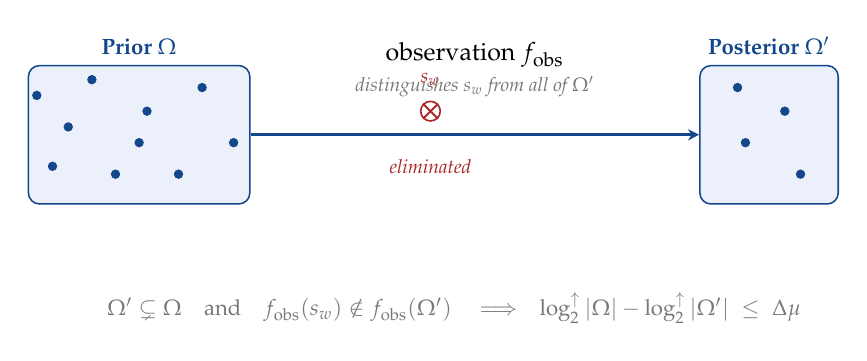
\begin{tikzpicture}[thiele]
% Prior set on the left
\node[
  draw=thiele@accent, line width=0.55pt,
  rounded corners=4pt,
  fill=thiele@pale,
  inner sep=10pt,
  minimum width=8em,
  minimum height=5.0em,
  align=center,
  label={[font=\footnotesize\bfseries, text=thiele@accent]above:Prior $\Omega$}
] (prior) at (0,0) {};
% Dots inside prior
\foreach \x/\y in {-1.3/0.5, -0.6/0.7, 0.1/0.3, 0.8/0.6,
                   -1.1/-0.4, -0.3/-0.5, 0.5/-0.5, 1.2/-0.1,
                   -0.9/0.1, 0.0/-0.1} {
  \node[circle, fill=thiele@accent, inner sep=1.2pt] at ($(prior.center)+(\x,\y)$) {};
}

% Posterior set on the right
\node[
  draw=thiele@accent, line width=0.55pt,
  rounded corners=4pt,
  fill=thiele@pale,
  inner sep=10pt,
  minimum width=5em,
  minimum height=5.0em,
  align=center,
  label={[font=\footnotesize\bfseries, text=thiele@accent]above:Posterior $\Omega'$}
] (post) at (8.0,0) {};
% Dots inside posterior (fewer, only those that survived)
\foreach \x/\y in {-0.4/0.6, 0.2/0.3, -0.3/-0.1, 0.4/-0.5} {
  \node[circle, fill=thiele@accent, inner sep=1.2pt] at ($(post.center)+(\x,\y)$) {};
}

% Eliminated state (crossed out, shown between)
\node[font=\scriptsize, text=thiele@red] at (3.7, 0.7) {$s_w$};
\node[circle, draw=thiele@red, line width=0.6pt, inner sep=2.5pt] (sw) at (3.7, 0.3) {};
\draw[thiele@red, line width=0.7pt] (sw.south west) -- (sw.north east);
\draw[thiele@red, line width=0.7pt] (sw.north west) -- (sw.south east);
\node[font=\scriptsize\itshape, text=thiele@red] at (3.7, -0.4) {eliminated};

% Big middle arrow with f_obs label
\draw[->, line width=1.0pt, draw=thiele@accent] (prior.east) -- (post.west)
  node[midway, above=1.0em, font=\small, align=center]
  {observation $f_{\text{obs}}$\\\scriptsize\itshape\color{thiele@gray} distinguishes $s_w$ from all of $\Omega'$};

% Bottom inequality
\node[font=\footnotesize, text=thiele@gray, align=center] at (4.0, -2.2)
  {$\Omega' \subsetneq \Omega$\quad and\quad
   $f_{\text{obs}}(s_w) \notin f_{\text{obs}}(\Omega')$
   \quad$\Longrightarrow$\quad
   $\log_2^{\uparrow}|\Omega| - \log_2^{\uparrow}|\Omega'| \;\leq\; \Delta\mu$};
\end{tikzpicture}
\caption{Schematic feasible-list narrowing under the representation theorem's premises. The strict subset and distinguishing observation support a stronger posterior predicate; the supplied fiber cover and numeric tree-payment premise are also required for the displayed bound. The expression $\log_2^{\uparrow}|\Omega|-\log_2^{\uparrow}|\Omega'|$ is a rounded list-size difference, not an assertion that the VM asked that many questions or that the lists contain that many distinct states.}
\label{fig:feasible-narrowing}
\end{figure}

\begin{theorem}[Feasible narrowing becomes predicate strengthening]
Suppose a posterior feasible set $\Omega'$ is a strict subset of a prior feasible set $\Omega$. Suppose also that an observation distinguishes a removed state from all posterior states. Then the membership predicate for $\Omega'$ is strictly stronger than the membership predicate for $\Omega$. (The membership predicate for $\Omega$ is the function that takes a state and returns true exactly when the state is in $\Omega$.)
\end{theorem}

\begin{proof}
Define $P_\Omega(s) := (s \in \Omega)$ and $P_{\Omega'}(s) := (s \in \Omega')$. ``Strictly stronger'' has two parts.

\emph{(a) $P_{\Omega'}$ implies $P_\Omega$.} If $P_{\Omega'}(s)$ holds, then $s \in \Omega'$. Since $\Omega' \subseteq \Omega$, we get $s \in \Omega$. So $P_\Omega(s)$ holds.

\emph{(b) $P_\Omega$ does not imply $P_{\Omega'}$.} Since $\Omega' \subsetneq \Omega$, there exists $s_w \in \Omega \setminus \Omega'$. So $P_\Omega(s_w)$ is true and $P_{\Omega'}(s_w)$ is false. That is enough for strictness. The distinguishing observation gives more: an explicit Boolean function witnessing $s_w$, not just the assertion that some such state exists. \qed
\end{proof}

\begin{plainreading}
Smaller set, stronger predicate. That is the whole of (a), and it is pure set inclusion doing the work. (b) is where the distinguishing observation earns its rent. Without it you have an existential: somebody, somewhere, lives in the gap. With it you have a name and an address. An existential is a promise. A witness is the proof of the promise.
\end{plainreading}

It feels like two separate things happened. First you did some work and the search space got smaller; then, as a reward, you got to assert something stronger. Two events, cause and effect, the second one earned by the first. That ordering is the illusion. There is no second event. The instant $\Omega$ shrinks to $\Omega'$ the stronger predicate already exists, because the predicate is nothing but membership in the set, and the set is smaller. Nobody pulled the predicate out of a hat to make the theorem go through; it was sitting there the whole time, defined by the boundary that just got redrawn. The distinguishing observation is what lets you write the boundary down honestly, but it does not author a new claim on top of the narrowing. The narrowing is the claim. One fact wearing two costumes: shrink the feasible set and tighten the predicate are the same move read off opposite sides of the same equation.

\begin{theorem}[Strengthening requires structure addition]
If a trace starts with no certification address, ends certified for a strictly stronger predicate, and that certification is tied to the supra-certification channel defined above, then the trace contains a structure-addition event.
\end{theorem}

\begin{proof}
``No certification address at start'' is $s_0.\texttt{vm\_csrs}.\texttt{csr\_cert\_addr} = 0$. ``Certified for the supra-cert channel at end'' is $s_n.\texttt{vm\_csrs}.\texttt{csr\_cert\_addr} \neq 0$, the definition of \texttt{has\_supra\_cert}. The trace runs from $s_0$ to $s_n$ through a finite sequence of steps. The field $\texttt{csr\_cert\_addr}$ starts at $0$ and ends nonzero. Somewhere in the trace, it flipped. That step is, by the definition in Section~\ref{sec:entitlement}, a structure-addition event. The strictly-stronger-predicate hypothesis names what the certification is \emph{for}; it does not affect the existence of the flip. \qed
\end{proof}

\begin{plainreading}
Cert address starts at $0$, ends nonzero. So somewhere along the trace, it flipped. That flip IS what we defined ``structure-addition event'' to be in Section~\ref{sec:entitlement}. The proof is just observing: if the value went from $0$ to nonzero across a finite trace, the change happened on some specific step. The mathematics is bookkeeping.
\end{plainreading}

This is the formal answer to ``where did the new admissible structure enter?'' Arithmetic on its own never answers that, because arithmetic only ever hands back what was already derivable from what you fed it; it closes a question, it does not open the world up to a fact that was not already in the premises. A stronger admissible predicate is exactly such a new fact, so it could not have fallen out of the computation for free. It had to be added, and the theorem says where: not in a flourish at the end, not off the page, but at one specific step you can point to in the trace, a structure-addition event with a timestamp.

\begin{theorem}[Universal certification cost]
Take any abstract computational system: states, step labels, step rule, cost function, certification predicate. If every one-step move from uncertified to certified costs at least 1, then every trace from uncertified to certified has total cost at least 1.
\end{theorem}

\begin{proof}
This is the same theorem as the Universal No Free Certification result in Section~\ref{sec:nofi}, restated here at the structural-entitlement layer. The proof is the trace-induction argument given there. Empty trace cannot flip the cert predicate. A non-empty trace either flips it at the first step, where single-step A2 gives $\geq 1$, or flips it later, where the induction hypothesis gives $\geq 1$ on the rest. Either case yields total cost $\geq 1$. \qed
\end{proof}

\begin{plainreading}
This is the same theorem as the one in the NoFI section, carried up here on purpose. Down there it was proved as a fact about cost. Up here the structural-entitlement layer needs that same floor as one of its own load-bearing parts, not as a footnote pointing back down the page, because the whole argument about who gets to claim a stronger predicate stands on it: certification never comes free wherever A2 is in force. Accept A2 and you have already agreed that flipping certification on costs you something. A2 acceptance is the entry fee.
\end{plainreading}

This theorem matters because it is not about the 51-opcode ISA. The cost floor is forced for any system the moment that system has a certification predicate and a cost rule that charges for certification transitions. Build the predicate so it can flip at zero cost and you have free certification by construction. And a system that refuses to represent certification at all has no way to talk about structural entitlement from the inside. The entitlement gets smuggled in from outside, and somebody signs their name to it. Smuggled entitlement is not entitlement, no matter whose name is on it.

\begin{theorem}[Structural entitlement representation]
For any values satisfying the explicit Coq premises of \code{structural\_entitlement\_representation}, consisting of:
\begin{itemize}
\item a strict feasible-set narrowing $\Omega' \subsetneq \Omega$;
\item an observation function that distinguishes at least one eliminated witness state from all posterior states;
\item a \texttt{Certified} posterior predicate built from the specified decoder, observation equality, and membership in $\Omega'$; in this theorem \texttt{Certified} includes the VM's \texttt{has\_supra\_cert} condition, whereas the separate observation-level theorem uses \texttt{CertifiedObs};
\item a decision tree \emph{realized by the trace}: the tree's depth is bounded by the count of cert-setter instructions the trace executes (\code{decision\_tree\_realized\_by\_trace}, defined as $\mathrm{depth}(T) \leq \texttt{cert\_setter\_executions}$). This is a payment bound on depth, a scalar comparison, not a claim that the trace's step sequence is mapped node-by-node onto the tree's branches; and
\item a posterior-representative reduction tying each prior list entry to a posterior representative with equal observation, together with the explicit fiber-size bound that yields $|\Omega| \leq \mathrm{leaves}(T)|\Omega'|$,
\end{itemize}
the posterior predicate is strictly stronger than the prior predicate, the trace contains a structure-addition event, and the size of the narrowing is bounded by the paid ledger:
\[
\log_2^{\uparrow}|\Omega| - \log_2^{\uparrow}|\Omega'| \leq \Delta \mu.
\]
Here $|\Omega|$ means the length of the prior feasible list, using the $|\cdot|$ notation from Section~\ref{sec:vocab}. $\Omega$ is a plain \texttt{list VMState}, not deduplicated and not a Coq \texttt{set}; $|\Omega|$ counts list entries, duplicates included, not distinct states. Nothing below assumes $\Omega$ is duplicate-free. $|\Omega'|$ is the posterior list's length, on the same convention. $\log_2^{\uparrow}$ means: take the base-2 logarithm and round up. A 1000-entry list needs 10 yes-or-no questions to pin down one entry, because $2^{10}=1024$, the first power of two that can cover 1000 items. That is the intuition, and only the intuition. The VM did not ask those questions. This is not Shannon entropy. With duplicates in the list, it is not a count of distinct states either. Both sides of the bound are integers. The eye wants to read $\log_2^{\uparrow}|\Omega| - \log_2^{\uparrow}|\Omega'|$ as the textbook bit-gain $\log_2(|\Omega|/|\Omega'|)$, and that is the one reading to set aside: the two ceilings round separately, so the difference can land above that real-valued number or below it. The proof bounds the integer itself, through the supplied fiber cover and the tree's depth, and the depth by the cert-setter payment. $\Delta\mu$ is final $\mu$ minus initial $\mu$ across the bounded trace.
\end{theorem}

\begin{proof}
Three conclusions, chained.

\emph{(i) Strictly stronger predicate.} The strict narrowing $\Omega' \subsetneq \Omega$ and the distinguishing observation match the hypotheses of the theorem above. Apply it. The membership predicate of $\Omega'$ is strictly stronger than that of $\Omega$.

\emph{(ii) Structure-addition event.} By hypothesis, the posterior certification uses the supra-cert channel. So the trace starts with $\texttt{csr\_cert\_addr} = 0$ and ends with $\texttt{csr\_cert\_addr} \neq 0$. The Strengthening-requires-structure-addition theorem gives a structure-addition event at some step $k^*$.

\emph{(iii) The $\log_2^\uparrow$ bound.} The realized decision tree $T$ is binary; write $\ell$ for its leaf count. Sort the prior states by which posterior state they end at. That is $|\Omega'|$ groups, and the covering hypothesis (\code{tree\_covers\_feasible\_reduction}, itself discharged from the trace's fibered reduction by \code{fibered\_reduction\_implies\_tree\_cover}) caps every group at $\ell$ states. So $|\Omega| \leq \ell \cdot |\Omega'|$. Take $\log_2^\uparrow$ of both sides and use that it is subadditive on products, $\log_2^\uparrow(ab) \leq \log_2^\uparrow a + \log_2^\uparrow b$:
\[
\log_2^\uparrow|\Omega| \;\leq\; \log_2^\uparrow \ell + \log_2^\uparrow|\Omega'|,
\qquad\text{equivalently}\qquad
\log_2^\uparrow|\Omega| - \log_2^\uparrow|\Omega'| \;\leq\; \log_2^\uparrow \ell.
\]
A binary tree holds at most $2^d$ leaves at depth $d$, so $\log_2^\uparrow \ell \leq d$, and the two combine to
\[
\log_2^\uparrow|\Omega| - \log_2^\uparrow|\Omega'| \;\leq\; \log_2^\uparrow \ell \;\leq\; d.
\]
The realized-by-the-trace hypothesis is exactly the numeric bound $d \leq \texttt{cert\_setter\_executions}$: the tree's depth is charged against the count of cert-setter instructions the trace executes, not matched branch-by-branch against the trace's own step sequence. Section~\ref{sec:mu} charges each cert-setter step at least $1$ in $\mu$, so that many cert-setter steps cost at least that much total, and the total is at most $\Delta\mu$, the cost of the whole trace. Chain the inequalities:
\[
\log_2^\uparrow|\Omega| - \log_2^\uparrow|\Omega'| \;\leq\; d \;\leq\; \texttt{cert\_setter\_executions} \;\leq\; \Delta\mu. \qed
\]
\end{proof}

\begin{plainreading}
Three conclusions, three steps. Conclusion 1 is just the predicate-strengthening theorem, applied to the strict-narrowing and distinguishing-observation hypotheses. Conclusion 2 is just the structure-addition theorem, applied to the trace's start-uncertified, end-certified condition. Conclusion 3 is the entropy bound. A binary tree that compresses $|\Omega|$ states into $|\Omega'|$ leaf-classes has depth at least $\lceil \log_2(|\Omega|/|\Omega'|) \rceil$, bounded by $\log_2^\uparrow|\Omega| - \log_2^\uparrow|\Omega'|$ on the underestimate side. Each tree node is a certified observation. Each certified observation pays at least $1$ in $\mu$. The tree depth is bounded by $\Delta\mu$. Compression for less than you paid never shows up, because the ledger does not extend that kind of credit. The bound is not a price anyone gets to negotiate down; the universe already settled it.
\end{plainreading}

\begin{figure}[!htbp]
\centering
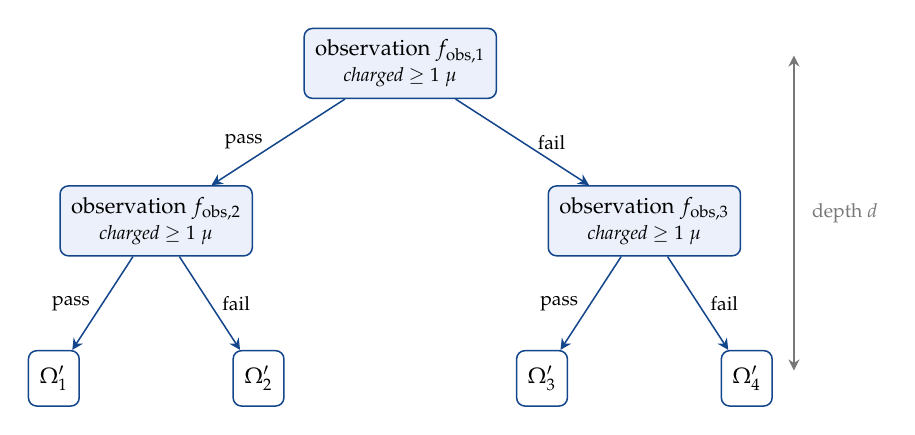
\begin{tikzpicture}[thiele,
  level distance=2.4em,
  sibling distance=10em,
  every node/.style={font=\small},
  treenode/.style={
    draw=thiele@accent, line width=0.55pt,
    rounded corners=3pt,
    fill=thiele@pale,
    inner sep=4pt,
    align=center,
    font=\footnotesize,
    minimum height=2.0em
  },
  leafnode/.style={
    draw=thiele@accent, line width=0.55pt,
    rounded corners=3pt,
    fill=white,
    inner sep=4pt,
    align=center,
    font=\footnotesize,
    minimum height=2.0em
  },
  treearrow/.style={->, line width=0.55pt, draw=thiele@accent}
]
% Root
\node[treenode] (root) at (0,0) {observation $f_{\text{obs},1}$\\\scriptsize\itshape charged $\geq 1\;\mu$};

% Level 1
\node[treenode] (l1) at (-3.1,-2.0) {observation $f_{\text{obs},2}$\\\scriptsize\itshape charged $\geq 1\;\mu$};
\node[treenode] (r1) at ( 3.1,-2.0) {observation $f_{\text{obs},3}$\\\scriptsize\itshape charged $\geq 1\;\mu$};

% Leaves
\node[leafnode] (ll) at (-4.4,-4.0) {$\Omega'_1$};
\node[leafnode] (lr) at (-1.8,-4.0) {$\Omega'_2$};
\node[leafnode] (rl) at ( 1.8,-4.0) {$\Omega'_3$};
\node[leafnode] (rr) at ( 4.4,-4.0) {$\Omega'_4$};

% Edges from root
\draw[treearrow] (root) -- node[left=2pt, font=\scriptsize] {pass} (l1);
\draw[treearrow] (root) -- node[right=2pt, font=\scriptsize] {fail} (r1);

% Edges from level 1 to leaves
\draw[treearrow] (l1) -- node[left=1pt, font=\scriptsize] {pass} (ll);
\draw[treearrow] (l1) -- node[right=1pt, font=\scriptsize] {fail} (lr);
\draw[treearrow] (r1) -- node[left=1pt, font=\scriptsize] {pass} (rl);
\draw[treearrow] (r1) -- node[right=1pt, font=\scriptsize] {fail} (rr);

% Depth annotation on the right
\draw[<->, line width=0.45pt, draw=thiele@gray]
  (5.0, 0.1) -- (5.0, -3.9)
  node[midway, right=3pt, font=\scriptsize, text=thiele@gray, align=left]
  {depth $d$};

\end{tikzpicture}
\caption{The decision tree witness. The tree is a branching skeleton; the observation and posterior-representative premises carry its semantic interpretation. The realised-by-the-trace condition bounds the tree's depth by the count of cert-setter executions, a numeric payment bound, not a claim that each node is individually matched to a specific step. The tree's depth bounds the feasible-set reduction on the right, and the $\mu$ paid for the trace bounds the depth on the left.}
\label{fig:decision-tree}
\end{figure}

This theorem does not quantify over the English word ``structure.'' It defines the witness class: strict narrowing, distinguishability, certification, and an explicit tree/fiber representative for the reduction. For every member of that class, structural entitlement is not metadata and not a slogan. It is predicate strengthening. It requires structure addition. Its quantified narrowing is charged to $\mu$. That is what entitlement means here. Not a feeling, not a story.

\begin{theorem}[Every sound structural shortcut lands here]
A \code{SoundStructuralShortcut} is a package containing exactly the receipts a shortcut must provide to count as sound: a prior feasible set, a posterior feasible set, strict narrowing, a distinguishing observation, a certified posterior predicate, a realized decision tree, and a posterior-representative reduction. For every such package, the structural-entitlement representation theorem applies. The shortcut lands in strictly stronger posterior knowledge, a structure-addition event, and the $\Delta\mu$ lower bound.
\end{theorem}

\begin{proof}
By construction, a \code{SoundStructuralShortcut} Coq record contains: $\Omega$, $\Omega'$ with $\Omega' \subsetneq \Omega$, an observation function $f_{\mathrm{obs}}$ with a distinguishing-witness proof, a decision tree $T$ with the numeric tree-payment obligation, a posterior-representative reduction with a representatives proof, and an initial-uncertified proof on the starting state. These fields and obligations are exactly the hypotheses of the Structural-Entitlement-Representation theorem. Project the seven data fields and eight proof obligations from the record into the theorem's hypotheses. Apply the theorem. The three conclusions (strictly stronger predicate, structure-addition event, $\log_2^\uparrow$-narrowing $\leq \Delta\mu$) follow. \qed
\end{proof}

\begin{plainreading}
The record is exactly what the representation theorem needs as input. Unpack the record. Plug the fields into the theorem. Read off the three conclusions. The class is non-empty because \code{factored\_n1\_shortcut} builds a member of the class on the page, by name. Non-empty by exhibition, not by reasoning.
\end{plainreading}

This is the formal version of ``it has to.'' Once a shortcut stops being a human story and becomes a sound object the substrate may use, it has to carry the data that makes it admissible. In this framework, that data is exactly the structural-entitlement witness. When symmetry, factorization, modularity, independence, or decomposition is named as the source of a shortcut, the next question is no longer mystical. It is a checklist: the prior set, the posterior set, the observation that rules something out, and the representative witness and tree witness. With those in hand the shortcut is admissible. Without them the structure is still sitting outside the computation, however good the story around it sounds.

\subsection{What narrowing buys}

There's a concrete version of all this you can run, a factored search problem built to make the difference visible. Two programs go after the same answer. The blind one runs with every instruction cost set to 0 and searches the flat space, paying nothing and seeing nothing, which is the point and not an accident: a machine with no ledger gets its blindness for free. The sighted one pays first. Two receipt-visible events, each \texttt{EMIT "." 0}, for a total receipt cost of 18, and only then does it split the problem into two factors and search them apart. That 18 is the whole tab. The kernel proves the exact cost formulas, and it proves the arithmetic that makes the trade lopsided: the $N^2$ versus $2N$ gap doesn't merely win, it eventually dwarfs that constant $\mu$ cost by orders of magnitude, so the price you paid up front stops mattering almost immediately. The executable tests run the actual VM at representative sizes and watch the measured numbers land where the proof says they will. The receipt costs 18 once. The exponent saves you forever.

The point of this example is not the $N^2$ versus $2N$ speedup. Divide-and-conquer is not the new claim. Nobody is selling that. The point is the auditable trace. The receipt-visible \texttt{EMIT} events plus the certified suffix satisfy the \code{SoundStructuralShortcut} witness contract, so the shortcut is admissible to the substrate, not just asserted by the programmer who happens to feel good about it. Admissible is all it is. The receipt does not prove the factorization is right. It does not authenticate a referee, and it does not tie the property label to a factorization checker. The 18 $\mu$ is the cost of the receipt-only trace; the extended trace costs 19 $\mu$ after the three-instruction certification suffix. The receipt is the evidence of what the trace paid for. Whether the math inside it is right is a separate question, and it needs its own proof.

There are two nearby claims here and it matters to keep them separate, because conflating them is exactly how a real theorem turns into a stage trick. The \texttt{EMIT}-only $N=1$ witness closes the observation layer. It proves posterior admissibility as \texttt{CertifiedObs} (a Coq type for ``a certified observation has been recorded,'' meaning the VM has observed and recorded a result but has not yet activated a cert channel). It does not close the stronger bridge. The trace does not end in \texttt{has\_supra\_cert}. In the semantic CSR-transition sense, it does not realize structure addition. Appending \texttt{PNEW}, \texttt{MORPH\_ID}, and \texttt{MORPH\_ASSERT} to the factorized search fires the concrete certification channel and places the resulting trace within the full structure-addition theorem.

That example is not a P vs NP result. Anybody who reads it as one is reading their own ambition into the bytes. It is a small, honest witness for what the substrate is meant to track. Certified structure can change which computation is admissible. The cost of acquiring that admissibility is not the same as the time saved by using it. One is the entry fee. The other is the dividend.

\medskip
\noindent\textbf{What the package looks like in the concrete \texttt{n=1} witness.} It pays to lay the whole package open once, at the smallest factored-search case, where the object is small enough to count on your fingers and nothing has to be taken on faith. The record \code{SoundStructuralShortcut} carries fifteen fields. Seven are data: decoder, observation fn, representative observation fn, observation equality, prior set, posterior set, decision tree. The other eight are proof obligations standing over that data, the receipts that say the data behaves the way the fields promise. The nine semantic ingredients below cover six of the seven data fields, the decoder being the identity map and living in the wiring, plus five of those obligations: strict narrowing, the distinguishing observation, tree realization, the certified posterior, and the initial-uncertified state. The remaining three obligations are discharged inline by the wiring that holds the record together. Fifteen fields, nine ingredients, four pieces of wiring, and that is the whole of it. Nothing here is hand-waved, because there is no room left to wave a hand: every part has a place, and every place is filled.

\begin{enumerate}
\item \textbf{Prior feasible set $\Omega$.} \texttt{sighted\_n1\_supra\_prior := [init\_state; sighted\_n1\_supra\_final]}. A literal two-element list of \texttt{VMState} values.
\item \textbf{Posterior feasible set $\Omega'$.} \texttt{sighted\_n1\_supra\_posterior := [sighted\_n1\_supra\_final]}. A literal one-element list.
\item \textbf{Strict narrowing.} $|\Omega'| = 1 < 2 = |\Omega|$ by direct inspection of the lists.
\item \textbf{Distinguishing observation.} \code{sighted\_n1\_supra\_obs\_fn}. Returns \code{sighted\_n1\_supra\_trace} when \texttt{vm\_mu = 19}, else \texttt{[]}. The post-\texttt{MORPH\_ASSERT} state has \texttt{vm\_mu = 19}. The initial state has \texttt{vm\_mu = 0}. The observation separates them.
\item \textbf{Decision tree.} \texttt{sighted\_n1\_tree := dt\_branch dt\_leaf dt\_leaf}. A two-leaf branching tree, one branch per factor.
\item \textbf{Tree realized by the trace.} The closed witness supplies the numeric premise \code{decision\_tree\_realized\_by\_trace}: the tree depth is at most the number of cert-setter executions in the bounded run. The theorem does not claim that the trace's opcode sequence is a node-by-node traversal of the tree.
\item \textbf{Posterior-representative reduction.} \code{sighted\_n1\_supra\_repr\_obs\_fn}. Defined as \texttt{if Nat.eqb s.(vm\_mu) s.(vm\_mu) then [] else [instr\_halt 0]}; the tautology \texttt{Nat.eqb mu mu = true} always picks the empty-list branch, so this is the empty-observation representative dressed up as a conditional.
\item \textbf{Certified posterior predicate.} Built from \code{omega\_predicate receipt\_list\_eqb sighted\_n1\_supra\_posterior sighted\_n1\_supra\_obs\_fn}. The \texttt{MORPH\_ASSERT} in the supra-suffix activates the VM's certification channel, which is the channel premise used by the formal package; it does not check the mathematical factorization named in the surrounding prose.
\item \textbf{Initial uncertified state.} \code{init\_state.(vm\_csrs).(csr\_cert\_addr) = 0} by definition of \texttt{init\_state}.
\end{enumerate}

All of that machinery only earns its keep if something actually satisfies it, and the worry with any definition this elaborate is that you have quietly written down a shape nothing in the world fits. So the lemma \code{sound\_shortcut\_from\_components} does the unglamorous thing: it takes the seven data fields listed above and eight proof hypotheses, one per obligation, and out the other end comes a \code{SoundStructuralShortcut} record. Then the closed term \code{factored\_n1\_shortcut : SoundStructuralShortcut 33 sighted\_n1\_supra\_trace init\_state} feeds it the seven fields and clears each of the eight obligations with a named lemma, and the downstream theorem \code{factored\_n1\_shortcut\_lands\_in\_representation} runs \code{every\_sound\_structural\_shortcut\_lands\_here} over that finished term and reads back exactly what the abstract class promised: a strictly stronger posterior predicate, a structure-addition event, and the $\log_2^{\uparrow}$ narrowing bounded by $\Delta\mu$. The payoff is small to state and it is the one I actually cared about. The class is not empty, and it is non-empty by construction, not by argument: there is a concrete shortcut built on the page that hits every clause, which means the whole apparatus is about something real and not a definition admiring itself in a mirror.

\subsection{The boundary}

The hard internal theorem for the explicit class is proven, and so is the boundary in both directions on a concrete witness. An \texttt{EMIT}-only factorized-search trace closes only the observation layer. The posterior predicate is certified observationally. But the trace does not reach \texttt{has\_supra\_cert} and does not realize semantic structure addition. A trace with the factorized search unchanged and a post-search suffix \texttt{PNEW ; MORPH\_ID ; MORPH\_ASSERT} closes the whole chain: stronger predicate, structure addition, and the $\Delta\mu$ lower bound. An unconditional Shannon-style bound on every deterministic single trace is something the code refuses to claim. A single execution path is not enough information. The bound needs the whole tree, or a per-branch preimage, or a distribution over traces. The proof stops where the witness stops. That is the honest place to stop, not a hole to be patched later.

Once entitlement is internalized with explicit witnesses instead of waved at, the picture firms up into three facts that lean on each other. You cannot strengthen a certified claim for free: the receipt costs $\mu$ or it does not exist. Strip a trace down to its classical shadow and the distinctions that entitlement turns on stop being visible at all, so the shadow can no longer tell you what was earned and what was merely assumed. And narrowing the feasible set is no longer a vibe; it has a formal path into predicate strengthening with a ledger lower bound underneath it, so the act of knowing more shows up as a number that went up. Then the substrate-level result in Section~\ref{sec:substrate-undecidability} settles the question you would ask next, which is whether all of this can be put on autopilot: is there a uniform, internally representable, always-terminating procedure that takes a formalized structural argument and hands back a \code{SoundStructuralShortcut} witness whenever a sound one exists? There is not; Section~\ref{sec:substrate-undecidability} constructs the reduction. A partial procedure, restricted to some class of arguments or free to decline rather than terminate, is not what that reduction rules out. The structural axis comes with its own undecidable predicate, in that total-procedure sense, which is the unsurprising and slightly bleak news that insight does not reduce to a crank you can turn.

%===========================================================================
\section{What insight is, and why it cannot be free}
\label{sec:insight}
%===========================================================================

On this substrate the word \emph{insight} stops being a mood and starts having a meter reading. It comes in three tiers, three genuinely different things that happen when a computation learns, and they sort themselves by price: the first can be free, the second never is, and the third is where the price tag has its hand on a certified game result that no single fixed classical strategy can produce.

\subsection{The three tiers of observation}

The kernel proves each tier lands where it lands, by what the substrate makes it cost, so the split is the substrate's verdict and not my filing system. Cheapest first.

\medskip
\noindent\textbf{Tier 0: Raw observation (free at $\delta=0$).}
A raw observation takes something in, writes it down, and stops there. It does not say what the data means, does not lean on it, and does not let any later step lean on it either. The cleanest case in the realisation is a CHSH trial, one round of the two-player game I build from scratch in Section~\ref{sec:chsh}: you run the round, a counter ticks up by one, and the certification channels stay cold. Nothing has been claimed, so there is nothing to commit to. The trial's cost is whatever $\delta$ it carries. At $\delta = 0$ the ledger does not move; with a positive $\delta$ it is charged and it is still Tier 0. So looking can be free on this substrate. You can watch as long as you like at $\delta = 0$ and the meter never starts. That is a fact about this machine's cost schedule, not a claim that looking is free in the physical world. The meter starts the instant you turn what you saw into something you are willing to stand behind, and that instant is a different tier.

\medskip
\noindent\textbf{Tier 1: Certified structural insight (always costs $\geq 1$).}
Two cert channels. \texttt{csr\_cert\_addr} (the formula/certificate address, a control-status register; Section~\ref{sec:formal} explains the term). \texttt{vm\_certified} (the top-level flag). Any concrete instruction that turns either channel from off to on costs at least 1. The kernel proves it: \code{certification\_requires\_positive\_mu}.

Precision first. \texttt{LASSERT} reads a constraint package and charges for it. \texttt{LASSERT} does not flip either cert channel. Two opcodes do the flipping: \texttt{CERTIFY} (sets \texttt{vm\_certified = true}) and \texttt{MORPH\_ASSERT} (sets \texttt{csr\_cert\_addr} nonzero when the assertion succeeds). \texttt{LASSERT} is the validation that precedes them. The kernel groups a broader cost-positive class: \texttt{LASSERT}, \texttt{EMIT}, \texttt{REVEAL}, \texttt{LJOIN}, \texttt{READ\_PORT}, \texttt{CERTIFY}, \texttt{MORPH\_ASSERT}, and the five-opcode \texttt{CHSH\_LASSERT} check family (Section~\ref{sec:isa} builds it). Each costs at least 1 at the step level. \texttt{LASSERT} is part of the chain. The cert-channel flip happens at the subsequent \texttt{CERTIFY} or \texttt{MORPH\_ASSERT}, not at \texttt{LASSERT} itself.

The chain, written out. Readers collapse two steps into one. Don't. Suppose register \texttt{r0} holds the address of a four-byte formula in memory and \texttt{r1} holds the address of a dual-witness certificate (a satisfying assignment together with a falsifying assignment, the non-triviality witness from Section~\ref{sec:isa}). Step one: \texttt{LASSERT freg=r0 creg=r1 kind=SAT flen=4 delta=0} reads the formula header, walks the formula and the two witnesses through the on-chip Logic Engine, charges $4 \times 8 + 1 = 33$ to $\mu$, and either advances the PC (validation passed) or traps to \texttt{LASSERT\_TRAP\_PC} and latches \texttt{vm\_err = true} (validation failed). The $\mu$ cost is charged either way. Both \texttt{csr\_cert\_addr} and \texttt{vm\_certified} stay untouched by this step, validation passing or not. Step two, conditional on step one passing: \code{MORPH\_ASSERT mid=m property="validated\_constraint" cert="" delta=0} charges $S(0) = 1$ to $\mu$ ($S$ is successor, $S(n) = n + 1$; Section~\ref{sec:mu} builds the notation properly) and flips \texttt{csr\_cert\_addr} to the ASCII checksum of \code{"validated\_constraint"}, which is nonzero because the property string carries non-NUL bytes. The supra-cert channel is now active.

Total cost across the two steps: 34 $\mu$. \texttt{LASSERT} paid for the validation work. \texttt{MORPH\_ASSERT} paid for the channel flip. The cert channel only crossed from 0 to nonzero on the second step, not the first. The two costs are not redundant. One is the cost of checking the constraint package against its dual witness. The other is the cost of committing to the result of that check by activating the cert channel.

That two-step shape is a protocol the program author chooses to follow, not a dependency the two opcodes enforce on each other. \texttt{MORPH\_ASSERT} checks only that \texttt{mid} names an existing morphism; it does not read, and has no way to read, whether a \texttt{LASSERT} executed earlier in the same trace, on the same formula the property string names. Nothing stops a program from calling \texttt{MORPH\_ASSERT mid=m property="validated\_constraint" cert=""} directly, with no \texttt{LASSERT} anywhere in its history, and getting the identical channel-active state and the identical checksum for the identical 34-$\mu$-shaped cost if it pads with an equivalent no-op charge. \texttt{csr\_cert\_addr} nonzero means only that some \texttt{MORPH\_ASSERT} fired on an existing morphism with a non-NUL-byte property string; it does not mean a specific formula was checked, and the property string is a label, not a proof obligation the opcode verifies against anything. A downstream predicate that references \texttt{csr\_cert\_addr} and relies on ``the validated constraint the LASSERT step checked'' is relying on the trace having actually been built in the two-step shape above, a fact about how the program was written, not a fact \texttt{MORPH\_ASSERT}'s own semantics establish. Skipping \texttt{LASSERT} does not break a chain the kernel checks; it breaks a discipline the surrounding program was supposed to follow.

\medskip
\noindent\textbf{Tier 2: Certified binary-game witness insight (always costs $\geq 1$).}
The sharpest case, and it is worth slowing down on why it is sharp. Here the trace is certified and its CHSH statistics show $S$ pushed past 2, the classical ceiling (Section~\ref{sec:chsh} builds the game and the ceiling from nothing). The certification on its own is already a Tier 1 event, so it already costs at least one. But look at what is being certified. $S > 2$ on a finite tally rules out any single fixed deterministic strategy replayed identically at every recorded trial (Section~\ref{sec:chsh}'s finite-tally remark); a fixed-$\lambda$ shared-randomness-then-local-choice story of that narrow, unvarying kind cannot produce it. Reading the violation as ruling out local hidden variable models generally, the idealized-correlator claim Section~\ref{sec:chsh} actually proves, needs enough trials that the tally and the population correlation have converged; a short run from a genuinely randomized local model can land past 2 by chance, as the same section's coin-flip example shows. So this tier certifies a fact that constrains the space of classical explanations, more sharply as the trial count grows, and the price does not flinch for the size of the thing it is pricing. Certified evidence of a game violation costs at least one to come by, on a trace of any length you care to run.

\subsection{Why insight cannot be free}

The proof:

Suppose a trace starts in an uncertified state and ends in a certified state. Somewhere in that trace, a specific opcode fired that flipped one of the certification registers from off to on. The two concrete cert-channel instructions writing \texttt{vm\_certified} or \texttt{csr\_cert\_addr} are: \texttt{CERTIFY} (which sets \texttt{vm\_certified = true}) and \texttt{MORPH\_ASSERT} when the morphism exists (which sets \texttt{csr\_cert\_addr} to the ASCII checksum of the property string: nonzero for any property string with a non-NUL byte). These are the only instructions that change those fields. \texttt{CHSH\_LASSERT} sits in the certification cost-discipline class ($S(\delta) \geq 1$) but does not write to \texttt{vm\_certified} or \texttt{csr\_cert\_addr}. Its success is observable via PC advance and \texttt{vm\_err} staying false (the bridge theorem operates on that signature). \texttt{MORPH\_ASSERT} with an empty property string or a missing morphism does not activate the cert channel, though it still costs $S(\delta) \geq 1$. This is proven by case analysis over all 51 opcodes. Every other instruction leaves those fields unchanged. So: the cert flip happened at a \texttt{CERTIFY} or \texttt{MORPH\_ASSERT} step. Look at that exact step. That step, by the semantics of the 51-opcode VM, has cost $S(\delta) \geq 1$, because both \texttt{CERTIFY} and \texttt{MORPH\_ASSERT} are in the mandatory-floor class. So at that step: $\mu_{\text{after}} = \mu_{\text{before}} + S(\delta) \geq \mu_{\text{before}} + 1$. And because $\mu$ never decreases (each instruction adds a non-negative cost), $\mu_{\text{before}} \geq \mu_{\text{initial}}$. Therefore $\mu_{\text{final}} \geq \mu_{\text{after}} \geq \mu_{\text{before}} + 1 \geq \mu_{\text{initial}} + 1$.

This is a property of the specified step and cost rules, proved by case analysis and trace induction. It establishes that a certification transition cannot be free in this model. Semantic truth is a separate obligation: a paid flag alone proves no proposition, and a checker may be sound independently of a charging convention.

But cost alone is not yet semantic depth. A concrete realisation can spend resources checking a claim that turns out to be shallow. \texttt{LASSERT} does not count as structural certification merely because a formula parses and one satisfying assignment exists. It also requires a non-tautology witness: one satisfying assignment and one falsifying assignment. Under checker soundness, that proves the encoded formula is satisfiable and not a tautology. It does not, by itself, prove that the falsifying valuation is a state in the current prior feasible set, nor that the formula expresses a sound factorization or decomposition of the running problem. Those are separate representation and semantic obligations. The receipt proves spend; the witness proves only the stated formula property.

%===========================================================================
\section{\texorpdfstring{The $\mu$ ledger}{The mu ledger}}
\label{sec:mu}
%===========================================================================

$\mu$ (mu) is the global structural cost ledger of the Thiele substrate. One counter, carried by every state. Not the whole substrate. The part that keeps receipts.

More observables also do not automatically buy an additive bill. \code{joint\_floor\_is\_least} proves that the least natural-number charge satisfying a finite family of unit event floors is one whenever any event fires, and zero otherwise. A single unit can satisfy several floors at once. Two independent Boolean coordinates provide a concrete example. If I want their costs to add, I need a resource-accounting condition that actually makes them add. Coordinate independence alone does not do that work.

\subsection{What mu is}

$\mu$ is a single natural number riding along on every substrate state (a natural number being a non-negative integer, $0, 1, 2, \ldots$; the notation cheat sheet is in Section~\ref{sec:vocab}). It starts at 0 and it never goes down, and that second half is the whole character of the thing. A counter that can fall is an accountant you can lean on to revise the books. A counter that only ever climbs is a fact about history: it says how much has been spent, and it cannot be talked into saying less. $\mu$ is the second kind.

In the 51-opcode realisation, every instruction carries a cost parameter ($\delta$) in its encoding. The VM adds that cost to $\mu$ when the instruction executes. Here is how $\delta$ is used in practice:

For \textbf{pure compute programs}, meaning programs that do arithmetic, load and store values, and jump, every instruction carries $\delta = 0$. The program I use as the concrete zero-cost comparison case, \texttt{blind\_program}, has this property: every instruction sits at $\delta = 0$. The proof that its total $\mu$-cost is zero is a direct calculation. For these programs, $\mu$ stays at 0 unless a positive-cost instruction fires.

For \textbf{certification and revelation instructions} (\texttt{CERTIFY}, \texttt{LASSERT}, \texttt{MORPH\_ASSERT}, \texttt{EMIT}, \texttt{REVEAL}, \texttt{LJOIN}, \texttt{READ\_PORT}, and the five-opcode \texttt{CHSH\_LASSERT} check family): the cost is at least 1, regardless of $\delta$. Even $\delta = 0$ still costs 1. The positive floor is part of this instruction schedule.

\texttt{CERTIFY} sets a persistent flag and charges $S(\delta)=\delta+1$. The first false-to-true transition is the event A2 prices. Subsequent executions still cost money under the VM schedule. Persistence of a flag does not by itself establish physical erasure: an implementation may retain the previous state elsewhere.

One is the least positive natural number. Choosing an additive mandatory floor of one gives $\delta+1$, but A2 alone also permits larger charges. The substitution theorems identify exact unit pricing relative to the designated flip count, not the entire VM instruction schedule or a unique physical unit.

Throughout this document, $S(n)$ means $n + 1$. The $S$ stands for ``successor'' in the basic math sense: the successor of $n$ is the next natural number after $n$. So $S(0) = 1$, $S(1) = 2$, and so on. $S(\delta) = \delta + 1$ is always at least 1. \texttt{EMIT}, \texttt{REVEAL}, and \texttt{READ\_PORT} go further: their cost also grows with the information content they carry. An \texttt{EMIT} of one ASCII character (which is 8 bits, see Section~\ref{sec:vocab}) with $\delta = 0$ costs $8 + 1 = 9$. Ten characters costs $80 + 1 = 81$. Emitting more costs more. The price tracks the bits, every time, and there's no rate to negotiate.

For \textbf{everything outside that positive-cost class}, including \texttt{ADD}, \texttt{LOAD}, \texttt{STORE}, \texttt{JUMP}, \texttt{PNEW}, \texttt{PSPLIT}, \texttt{PMERGE}, \texttt{MORPH}, \texttt{COMPOSE}, and the rest, the VM charges exactly $\delta$, which can be 0. Here is why these are allowed to be free.

The schedule permits module operations at $\delta=0$. This is a design choice, not a derived thermodynamic statement. In particular, a zero-cost \texttt{PNEW} can change the graph, so positive cost for every observable structural change would be false for this VM.

Graph construction and assertion have different charges in this schedule. A physical interpretation would need a model of information-bearing states, operation boundaries, retained history, and dissipation; these cannot be inferred from opcode names or from graph changes alone.

$\mu$ grows whenever \texttt{instruction\_cost} is positive. The certification/revelation class is forced to be positive even when its encoded $\delta$ is 0. Other instructions can remain free by carrying $\delta = 0$.

Here is the complete cost schedule:

\medskip
\begin{center}
\begin{tabular}{@{}p{0.38\linewidth}p{0.55\linewidth}@{}}
\toprule
Instruction class & Cost = \texttt{instruction\_cost} \\
\midrule
Zero-floor operations (\texttt{ADD}, \texttt{LOAD}, \texttt{JUMP}, \texttt{PNEW}, \texttt{MORPH}, \ldots) & $\delta$ \quad (can be 0) \\
Certification floor (\texttt{CERTIFY}, \texttt{MORPH\_ASSERT}, \texttt{LJOIN}, the \texttt{CHSH\_LASSERT} family) & $S(\delta) = \delta + 1$ \\
\texttt{EMIT} (emit payload as receipt-visible trace event) & $|\text{payload}|_{\mathrm{bits}} + S(\delta)$ \\
\texttt{REVEAL} (disclose bits from a module) & $\text{bits} + S(\delta)$ \\
\texttt{READ\_PORT} (read bits from input port) & $\text{bits} + S(\delta)$ \\
\texttt{LASSERT} (validate formula and witnesses) & $\mathit{flen} \times 8 + S(\delta)$ \\
\bottomrule
\end{tabular}
\end{center}
\medskip

The $|\text{payload}|_{\mathrm{bits}}$ notation means ``the number of bits in the payload.'' A one-byte ASCII character contains 8 bits. A ten-byte string contains 80 bits.

For \texttt{LASSERT}: $\mathit{flen}$ is the number of formula units in the encoded formula. Each unit is one byte (8 bits) in the binary encoding used by the VM. This is a design choice in the binary format. The formula header declares how many bytes follow. The VM charges 8 bits per byte. The multiplication by 8 simply converts byte-count to bit-count, matching the information content you are asking the trace to validate.

The proof that $\mu$ is always exactly $\mu_{\text{before}} + \texttt{instruction\_cost}$ for each step:

\begin{theorem}[$\mu$-Conservation]
For any VM state $s$ and VM instruction $i$: $(\texttt{vm\_apply}\ s\ i).\mu = s.\mu + \texttt{instruction\_cost}\ i$.
\end{theorem}

\begin{proof}
Case analysis over the 51 opcode constructors of \texttt{vm\_instruction}. For each constructor $i$, the apply rule has the form
\[
(\texttt{vm\_apply}\ s\ i).\mu \;=\; s.\mu + c_i,
\]
where $c_i$ is the cost term written in the apply rule. Compare to \texttt{instruction\_cost}: for zero-floor opcodes $c_i = \delta$; for certification-floor opcodes (\texttt{CERTIFY}, \texttt{MORPH\_ASSERT}, \texttt{LJOIN}, and the \texttt{CHSH\_LASSERT} family, its four Q$_{1+AB}$ variants included) $c_i = S(\delta)$; for \texttt{EMIT} $c_i = |\text{payload}|_{\mathrm{bits}} + S(\delta)$; for \texttt{REVEAL} and \texttt{READ\_PORT} $c_i = \mathrm{bits} + S(\delta)$; for \texttt{LASSERT} $c_i = \mathit{flen} \times 8 + S(\delta)$. In every case $c_i$ matches the corresponding case of \texttt{instruction\_cost} by definition. The error sub-cases (e.g., \texttt{MORPH\_ASSERT} on a missing morphism, \texttt{CHSH\_TRIAL} with bad bits, \texttt{LASSERT} length mismatch) follow the same cost rule: the trap or err-latch only changes the PC and the error flag; the $\mu$ update is the same. So $(\texttt{vm\_apply}\ s\ i).\mu = s.\mu + c_i = s.\mu + \texttt{instruction\_cost}(i)$ for every $i$. \qed
\end{proof}

\begin{plainreading}
Look at each of the 51 opcodes one at a time. Every apply rule writes $\mu$ as the old $\mu$ plus the cost. The cost term is exactly what \texttt{instruction\_cost} returns. Including the error paths: failing an instruction costs the same as succeeding at it, because the cost is on the attempt, not the outcome. There is no opcode that escapes this. Every one of the 51 lands in the same equation.
\end{plainreading}

This is not a monotonicity claim. It is an equality. $\mu$ goes up by exactly the cost of the instruction, always, for every instruction, in every case including error cases. There is no backdoor.

That equality should not be misunderstood. It means the ledger is exact about spend. It does not, by itself, mean every paid unit corresponds to deep semantic gain. On this substrate, semantic gain is stricter than spend. It requires a narrowing witness in addition to the ledger entry.

\subsection{Why mu is the unique canonical cost measure}

Here is the stronger claim, which took a while before the proof compiled. $\mu$ is not just a valid cost measure for this 51-opcode realisation. It is the unique one. Any other cost function that starts at zero and tracks the per-instruction cost schedule exactly must equal $\mu$ on every reachable VM state. Not ``isomorphic'' in some abstract sense. Literally equal, value by value, on every reachable state.

\begin{theorem}[$\mu$-Initiality]
Let $M$ be any function from VM states to natural numbers satisfying: (a) $M$ assigns zero to the initial VM state, $M(\texttt{init\_state}) = 0$; and (b) $M$ tracks the cost schedule exactly: for every VM state $s$ and every VM instruction $i$, $M(\texttt{vm\_apply}\ s\ i) = M(s) + \texttt{instruction\_cost}(i)$. Then $M$ equals $\mu$ on every reachable VM state. (Monotonicity, the property that $M(s') \geq M(s)$ when $s'$ is reachable from $s$, follows from (b) because \texttt{instruction\_cost} is a non-negative natural number. You do not need to state monotonicity separately.)
\end{theorem}

\begin{proof}
Induction on the reachability witness for $s$. A reachable VM state is either $\texttt{init\_state}$ itself or $\texttt{vm\_apply}\ s'\ i$ for some reachable $s'$ and some VM instruction $i$.

\emph{Base case ($s = \texttt{init\_state}$).} By hypothesis (a), $M(\texttt{init\_state}) = 0$. By definition of the initial state in the kernel, $\texttt{init\_state}.\mu = 0$. So $M(\texttt{init\_state}) = \texttt{init\_state}.\mu$.

\emph{Step case ($s = \texttt{vm\_apply}\ s'\ i$ for reachable $s'$).} By hypothesis (b),
\[
M(s) \;=\; M(s') + \texttt{instruction\_cost}(i).
\]
By the induction hypothesis on $s'$, $M(s') = s'.\mu$. By $\mu$-Conservation,
\[
s.\mu \;=\; (\texttt{vm\_apply}\ s'\ i).\mu \;=\; s'.\mu + \texttt{instruction\_cost}(i).
\]
Substituting: $M(s) = s'.\mu + \texttt{instruction\_cost}(i) = s.\mu$. \qed
\end{proof}

\begin{plainreading}
$M$ agrees with $\mu$ at the start (both zero). The step rule says $M$ and $\mu$ both update by the same amount on every step ($M$ by hypothesis (b), $\mu$ by $\mu$-Conservation). Induction closes it. There is no alternative accounting that agrees with the cost schedule at every step, starts at zero, and disagrees with $\mu$ on a reachable VM state. The cost is forced.
\end{plainreading}

In plain language: given the cost schedule, there is no alternative accounting. If you charge $S(\delta)$ for certification-floor opcodes, $|\text{payload}|_{\text{bits}} + S(\delta)$ for \texttt{EMIT}, and $\delta$ for everything else, then $\mu$ is the only function on VM states that starts at zero and tracks the schedule. What was a design choice is the schedule itself: the decision that \texttt{CERTIFY} costs $S(\delta)$ and \texttt{ADD} costs $\delta$. But the schedule is not arbitrary either, and that is the part worth slowing down on. Hold the trust fixed and A2 is the only rule that prices certification exactly, so the only exact, non-overcharging substitute already \emph{is} A2 (\code{a2\_equal\_trust\_substitution\_payoff}). And $(\mu, \texttt{certified})$ is the proved-irredundant extension over (mem, regs, pc): cert is not a function of the rest, $\mu$ is not a function of the rest (\code{P\_full\_complete\_neither\_mu\_nor\_cert\_droppable}). A law that lives in the step is not a check you run afterward and hope you got right. Given-the-schedule uniqueness is the accounting; the A2-and-irredundancy result underneath it is the priority. No competing count can agree on the schedule, start at zero, and land on a different total, and there's nowhere left for that freedom to hide.

\subsection{The LASSERT cost formula}

The most important cost formula in the VM is for \texttt{LASSERT}, the opcode that validates a logical formula and its witnesses:

\[
\Delta\mu_{\text{LASSERT}} = \mathit{flen} \times 8 + S(\mathit{mu\_delta})
\]

$\mathit{flen}$ is the formula-unit count the instruction declares, and the declaration drives the bill: eight concrete bits per declared unit. The per-step mandatory charge is always at least 1, no matter how cheap the unit-count feels. What keeps the declaration honest is the header check below: the VM reads the count the formula's own in-memory header carries, and no validation succeeds unless the two agree.

What makes this the one to watch is where the bill gets keyed. The operand drives the charge, but no successful check ever underpays, because succeeding requires the declared count to equal the count sitting in the formula's own header. Eight bits for every unit, plus the floor of at least 1 you pay for the act of checking at all, and the act of checking is not up for negotiation. So a two-unit formula lands at 16 + 1 = 17, and there is no posture you can strike to talk it down: the formula's own header gives the true count, and a declaration that disagrees with it never validates anything. Declaring a smaller count does not shrink the formula; it only gets you caught. That is the whole reason you cannot smuggle a larger formula through a smaller bit count.

The minimum is relative to the stated formula-length charging constraints, as formalized by \texttt{cost\_necessity} and \texttt{cost\_uniqueness}. It is not a lower bound on all possible formula-validation algorithms or representations.

What this buys you: the trace pays for presenting and checking a constraint package, no more, no less. It does not, by itself, guarantee the constraint is meaningful. You could present a formula that is always true, a tautology, and the ledger would still charge you the full bill. The VM closes this separately via the dual-witness requirement: see the \texttt{LASSERT} opcode description in Section~\ref{sec:isa}.

\textbf{The obvious thing to try, and where it runs out.} The programmer declares $\mathit{flen}$ in the instruction encoding, so the first thing I wanted to know was: what stops them from writing $\mathit{flen} = 0$ for a huge formula and paying only $S(0) = 1$? It's the cheat I'd reach for first.

The VM catches it. When \texttt{LASSERT} runs, the VM reads the formula's actual encoded-unit count from the formula header in memory and compares it to whatever $\mathit{flen}$ the instruction claimed. If they do not match, the VM traps (Section~\ref{sec:vocab}: routes execution to a fixed error address): the program counter jumps to \texttt{LASSERT\_TRAP\_PC}, which is \texttt{0xF00} in hexadecimal, decimal 3840. The error flag is set. The check does not succeed. This trap-to-fixed-address behaviour belongs to \texttt{LASSERT} and to the \texttt{CHSH\_LASSERT} check family that inherits its discipline; every other error in the VM simply sets \texttt{vm\_err} to true and continues advancing the program counter by 1. The checks are special because a failed check of this kind is a serious integrity violation, not a recoverable error. The $\mu$ cost is still charged: that detail matters because failed checks are not free. The Coq lemmas \code{lassert\_honest\_cost} and \code{lassert\_honest\_mu\_cost} prove that if \texttt{LASSERT} completes without trapping, the declared count equals the in-memory count, and the $\mu$ charge uses the real formula bits.

%===========================================================================
\section{No Free Insight: the first cost law}
\label{sec:nofi}
%===========================================================================

\subsection{The abstract versions}

\begin{theorem}[Universal No Free Certification]
Let $\mathcal{C}$ be any abstract computational system with:
\begin{itemize}
\item a set of states;
\item a set of step labels;
\item a step rule (given a state and a step label, the rule produces the next state);
\item a cost function (each step label has a non-negative integer cost);
\item a certification predicate (a yes/no test on states, with at least one ``no'' state and at least one ``yes'' state).
\end{itemize}
Premise (A2, the single-step cost rule): for every state $s$ and step label $i$, if $\mathrm{cert}(s) = \mathrm{false}$ and $\mathrm{cert}(\mathrm{step}(s, i)) = \mathrm{true}$, then $\mathrm{cost}(i) \geq 1$.

Conclusion: any trace of step labels $t = [i_1, i_2, \ldots, i_n]$ that starts at state $s_0$ with $\mathrm{cert}(s_0) = \mathrm{false}$ and ends at state $s_n$ with $\mathrm{cert}(s_n) = \mathrm{true}$ has total cost $\sum_{k=1}^n \mathrm{cost}(i_k) \geq 1$.
\end{theorem}

\begin{proof}
Induction on the trace $t$.

\emph{Base case ($t = []$).} Then $s_n = s_0$, so $\mathrm{cert}(s_n) = \mathrm{cert}(s_0) = \mathrm{false}$. But the hypothesis says $\mathrm{cert}(s_n) = \mathrm{true}$. Contradiction; the empty-trace case is vacuous.

\emph{Step case ($t = i :: \mathrm{rest}$).} Let $s_1 = \mathrm{step}(s_0, i)$ be the state after the first step label. Case-split on $\mathrm{cert}(s_1)$.
\begin{itemize}
\item \emph{Subcase A: $\mathrm{cert}(s_1) = \mathrm{true}$.} The first step label flipped the certification predicate from false to true in one step. By the A2 premise, $\mathrm{cost}(i) \geq 1$. The total cost is $\mathrm{cost}(i) + \sum_{j \in \mathrm{rest}} \mathrm{cost}(j) \geq 1 + 0 = 1$, since every individual cost is a non-negative natural.
\item \emph{Subcase B: $\mathrm{cert}(s_1) = \mathrm{false}$.} Then the rest of the trace must do the flipping: $\mathrm{cert}(\mathrm{run}(\mathrm{rest}, s_1)) = \mathrm{true}$ with $\mathrm{cert}(s_1) = \mathrm{false}$. Apply the induction hypothesis at $(\mathrm{rest}, s_1)$ to get $\sum_{j \in \mathrm{rest}} \mathrm{cost}(j) \geq 1$. The total trace cost is $\mathrm{cost}(i) + \sum_{j \in \mathrm{rest}} \mathrm{cost}(j) \geq 0 + 1 = 1$.
\end{itemize}

Either subcase gives total trace cost $\geq 1$. \qed
\end{proof}

\begin{plainreading}
The cert predicate is off at the start, on at the end. So somewhere a step flipped it. Whichever step did the flipping costs at least 1 by the single-step rule. Every other step costs at least 0 because costs are non-negative naturals. Sum them up: at least 1. Empty trace can't do the flipping at all, so it's vacuous. That's the whole argument. The induction just makes precise the idea that the flip has to happen \emph{somewhere}, and wherever it happens it pays.
\end{plainreading}

This theorem does not know about registers, memory, partitions, morphisms, CHSH trials, or the 51-opcode ISA. It says: once a model has a yes/no certification test and the one-step certification transition is priced, trace-level non-free certification falls out by induction over the trace, no further premises required. If that one-step premise fails, the model permits free certification by definition. If the model has no certification predicate, it cannot talk about structural entitlement internally.

And don't read ``that's the whole argument'' as ``the premise is the whole content.'' The single implication is one line from the pricing rule, yes. The content is that this rule is the only one that fits. A trusted erasure-accounting law, the same trust posture, certifies at total cost zero when nothing is erased: a real rival, a different bill (\code{commitment\_cost\_not\_reducible\_to\_erasure\_cost}). And a substitute that charges any other predicate fails the floor on a one-step trace (\code{substitution\_test\_rejects\_non\_a2\_exact\_substitute}). A tautology does not get to have a rival that loses.

\begin{theorem}[Thiele No Free Insight]
For the 51-opcode VM specifically, cert-channel activation is positive-cost, and certified predicate strengthening has to pass through a structure-addition event. The relevant certification/revelation steps all live in the positive-cost class.
\end{theorem}

\begin{proof}
Two parts.

\emph{Cert-channel activation requires positive cost.} The Both-channels theorem below establishes that any trace activating either certification channel (\texttt{csr\_cert\_addr} becoming nonzero or \texttt{vm\_certified} becoming true) has $\Delta\mu \geq 1$. The actual channel-writing cases are covered by the positive-cost cert/revelation class: \texttt{CERTIFY}, \texttt{MORPH\_ASSERT}, \texttt{EMIT}, \texttt{REVEAL}, \texttt{LJOIN}, \texttt{LASSERT}, \texttt{READ\_PORT}, and the \texttt{CHSH\_LASSERT} family. The class is deliberately broader than literal field writers; every member has \texttt{instruction\_cost} $\geq S(\delta) \geq 1$, so the lower bound holds.

\emph{Certified predicate strengthening requires a structure-addition event.} By hypothesis the trace ends certified for a stronger predicate via the supra-cert channel (\texttt{csr\_cert\_addr} nonzero). The Strengthening-requires-structure-addition theorem (Section~\ref{sec:entitlement}) gives the structure-addition event directly. \qed
\end{proof}

\begin{plainreading}
This is just the abstract universal NoFI theorem instantiated for the 51-opcode realisation and read back through the Thiele substrate interface. The two concrete certification channels (\texttt{csr\_cert\_addr} and \texttt{vm\_certified}) are both cost-positive at the step level, and the predicate-strengthening reading of NoFI falls out of the structure-addition theorem.
\end{plainreading}

This is the VM-level version. The kernel proves the two concrete cert channels cannot be activated for free, by case analysis over all 51 opcodes, then adds the predicate-strengthening layer: once a stronger accepted predicate is tied to \texttt{has\_supra\_cert}, the trace must contain a structure-addition event somewhere in it.

\subsection{The specific versions}

For the 51-opcode VM concretely, there are several specific versions. The two certification channels I mentioned in Section~\ref{sec:insight} are the certificate-address register (\texttt{csr\_cert\_addr}) and the top-level flag (\texttt{vm\_certified}). Both are defined precisely in Section~\ref{sec:formal}, register by register.

\begin{theorem}[No Free Certification, single step]
If $s.\texttt{vm\_csrs}.\texttt{csr\_cert\_addr} = 0$ and $(\texttt{vm\_apply}\ s\ i).\texttt{vm\_csrs}.\texttt{csr\_cert\_addr} \neq 0$, then $\texttt{instruction\_cost}(i) \geq 1$.
\end{theorem}

\begin{proof}
Case analysis over the 51 opcode constructors. The Coq proof uses \texttt{cert\_addr\_setterb}: if \texttt{csr\_cert\_addr} changes from 0 to nonzero, the instruction must fall inside that cost-positive class. The class includes \code{instr\_morph\_assert}, \texttt{instr\_emit}, \texttt{instr\_reveal}, \texttt{instr\_ljoin}, and \texttt{instr\_lassert}. It is a deliberately broad guardrail class, not a list of literal CSR writers. In the current \texttt{vm\_apply} semantics, the direct CSR-writing success case is \code{instr\_morph\_assert}. For the theorem, the required fact is cost: every member of \texttt{cert\_addr\_setterb} has \texttt{instruction\_cost} $\geq 1$, with \texttt{instr\_emit} and \texttt{instr\_reveal} higher because they also charge payload bits. \qed
\end{proof}

\begin{plainreading}
If you see \texttt{csr\_cert\_addr} move from zero to nonzero, the proof catches that step inside a cost-positive guardrail class. That class is broader than the direct CSR writers, but broad is fine here: every member costs at least 1. The field cannot flip for free.
\end{plainreading}

\begin{theorem}[No Free Certification, trace level]
If a trace starts at a state with $\texttt{csr\_cert\_addr} = 0$ and ends at a state with $\texttt{csr\_cert\_addr} \neq 0$, then the trace's total $\mu$ cost is $\geq 1$.
\end{theorem}

\begin{proof}
Instantiate the universal theorem above with $\mathcal{C}$ = the 51-opcode VM; $\mathrm{cert}(s) := (s.\texttt{vm\_csrs}.\texttt{csr\_cert\_addr} \neq 0)$; $\mathrm{step}$ = \texttt{vm\_apply}; $\mathrm{cost}$ = \texttt{instruction\_cost}. The A2 premise is exactly the single-step theorem above. \qed
\end{proof}

\begin{plainreading}
Single-step lifts to trace-level. The universal theorem does the work.
\end{plainreading}

\begin{theorem}[No Free Certification via CERTIFY]
If a trace starts at a state with $\texttt{vm\_certified} = \mathrm{false}$ and ends at a state with $\texttt{vm\_certified} = \mathrm{true}$, then the trace's total $\mu$ cost is $\geq 1$.
\end{theorem}

\begin{proof}
Case analysis over the 51 opcodes shows that \texttt{vm\_certified} flips from false to true only when $i$ is an \texttt{instr\_certify} constructor; every other opcode leaves it unchanged. The \texttt{CERTIFY} apply rule charges $S(\delta) \geq 1$. So the single-step instance of A2 holds for this channel. Instantiate the universal theorem with $\mathrm{cert}(s) := s.\texttt{vm\_certified}$, otherwise as above. \qed
\end{proof}

\begin{plainreading}
Same shape as the other channel. Only one opcode (\texttt{CERTIFY}) can flip the top-level flag. It charges $\geq 1$. The universal theorem lifts that to the trace.
\end{plainreading}

\begin{theorem}[Both channels]
\label{thm:allchannels}
For ANY transition of either certification channel from absent to present, whether the certificate-address register \texttt{csr\_cert\_addr} or the top-level flag \texttt{vm\_certified}, $\mu$ grows by at least 1 over the trace.
\end{theorem}

\begin{proof}
Suppose the trace either flips \texttt{csr\_cert\_addr} from $0$ to nonzero, or flips \texttt{vm\_certified} from false to true (or both). In the first case the trace-level theorem (\texttt{csr\_cert\_addr}) applies. In the second case the trace-level theorem (\texttt{vm\_certified}) applies. The disjunction is exhaustive over ``cert-channel activation,'' so $\mu$ grows by $\geq 1$ in either case. \qed
\end{proof}

\begin{plainreading}
Two channels, one master claim. Whichever channel got activated, the corresponding single-step rule fired and the universal theorem lifted it to the trace. There is no third way.
\end{plainreading}

Theorem~\ref{thm:allchannels} is the one I actually reach for downstream. When something later in the document needs ``and certification was not free,'' this is the line it cites, because it has already done the bookkeeping of asking which way the certification came in and answered: doesn't matter, both are priced. The certificate-address register \texttt{csr\_cert\_addr} and the top-level flag \texttt{vm\_certified} are not two separate promises I have to keep track of; they collapse into one claim that holds no matter which door a program walks through to call itself certified.

\subsection{What this means in practice}

Run any program on the kernel. Watch the $\mu$ counter. If the program ends with \texttt{vm\_certified = true} or with \texttt{csr\_cert\_addr} nonzero, then somewhere in the trace, $\mu$ went up by at least 1. You can audit the trace and find exactly which opcode paid the bill. There is no program that can reach a certified state from scratch without paying for it.

On a valid execution from the initial state, a certified flag implies a positive accumulated charge. The ledger alone neither authenticates an externally supplied state nor proves an arbitrary proposition.

%===========================================================================
\section{The formal state record}
\label{sec:formal}
%===========================================================================

\begin{definition}[Concrete state record]
The kernel's \texttt{VMState} record realises the substrate state in 12 fields:
\begin{itemize}
\item $s.\texttt{vm\_graph}$: the partition graph. It contains module records, morphism records, and fresh-ID counters.
\item $s.\texttt{vm\_csrs}$: control-status registers. The hardware split: data registers hold values (like $s.\texttt{vm\_regs}$); CSRs hold configuration and status. Four fields:
 \begin{itemize}
 \item \texttt{csr\_cert\_addr}: 0 until something is asserted. Set to the ASCII checksum of the property string on a successful \texttt{MORPH\_ASSERT} (nonzero for any property string with a non-NUL byte). The name says address; the contents say fingerprint. Nonzero here means a structural property was certified and paid for.
 \item \texttt{csr\_status}: general status code. Informational. Nothing reads it; nothing branches on it.
 \item \texttt{csr\_err}: error code. Zero means clean. Nonzero means an instruction failed: bad argument, missing morphism, locality violation, etc.
 \item \texttt{csr\_heap\_base}: base address for \texttt{HEAP\_LOAD} and \texttt{HEAP\_STORE}. Final address = base + register-specified offset. No paging, no translation, just addition.
 \end{itemize}
\item $s.\texttt{vm\_regs}$: a list of register values. The kernel fixes \texttt{REG\_COUNT = 16}; reads and writes wrap modulo it. The kernel proofs are parametric in \texttt{REG\_COUNT}, so 16 is a scaffolding choice, not a theorem.
\item $s.\texttt{vm\_mem}$: a list of data-memory words. The kernel fixes \texttt{MEM\_SIZE = 128}; reads and writes wrap modulo it. The proofs are parametric here too.
\item $s.\texttt{vm\_pc} \in \mathbb{N}$: program counter. The integer that says \emph{which instruction next}.
\item $s.\texttt{vm\_mu} \in \mathbb{N}$: the $\mu$ ledger, the substrate's accounting field. Starts at 0. Never decreases.
\item $s.\texttt{vm\_mu\_tensor}$: a 4$\times$4 array of cost values (16 entries), indexed by direction pairs $(i,j)$. \texttt{REVEAL} is the one opcode that writes it, stamping the disclosure cost at the direction index encoded in the instruction; the per-module 4$\times$4 grids that \texttt{TENSOR\_SET} writes and \texttt{TENSOR\_GET} reads are separate state, carried inside \texttt{vm\_graph} (Section~\ref{sec:isa}). The kernel tracks \emph{where} costs land, not just how much. In the kernel model these are natural numbers; in the hardware, 32-bit words. If you don't use the tensor tracking, ignore all 16 entries.
\item $s.\texttt{vm\_err} \in \{\text{false}, \text{true}\}$: the error flag. Set when an instruction fails.
\item $s.\texttt{vm\_logic\_acc}$: a natural number with two roles. Role one: the Logic Engine accumulator during \texttt{LASSERT} (the on-chip unit that reads formula words and certificate bytes and tracks validation state). Role two: the magic key the FSM matches against. \texttt{0xCAFEEACE} (hex; 3{,}405{,}703{,}886 decimal) passes. Anything else, the FSM rejects. The field exists so the Coq kernel and the physical hardware agree on the same accumulator value at every step.
\item $s.\texttt{vm\_mstatus}$: status word, 0 or 1. 0 = Turing mode (ordinary computation; partition graph and morphism map idle). 1 = Thiele mode (structural state live). The kernel keeps this as a status indicator only. It does not gate the structural opcodes at the step level; those are always available. The field exists so the hardware and the Coq model agree across the bridge proofs.
\item $s.\texttt{vm\_witness}$: the CHSH witness counters. This is a record of 8 natural-number counters, one for each combination of (measurement setting pair) $\times$ (same/different outcome). The four setting pairs are $(x,y) \in \{(0,0),(0,1),(1,0),(1,1)\}$, where $x$ is Alice's setting and $y$ is Bob's setting. That is the modern Bell-test convention (NPA hierarchy, Brunner et al.\ 2014 review), and the same one the Coq constructor \texttt{instr\_chsh\_trial (x y a b : nat)} uses. The outcome variables are $(a, b)$. For each setting pair, there are two counters: same-outcome and different-outcome. Eight counters total: \texttt{wc\_same\_00}, \texttt{wc\_diff\_00}, \texttt{wc\_same\_01}, \texttt{wc\_diff\_01}, \texttt{wc\_same\_10}, \texttt{wc\_diff\_10}, \texttt{wc\_same\_11}, \texttt{wc\_diff\_11}, where the numeric subscript is the value of $(x, y)$ for that bucket. Each \texttt{CHSH\_TRIAL} instruction increments exactly one counter. (Some Bell-test literature uses the reverse convention with $(a,b)$ for settings; the numeric subscripts 00, 01, 10, 11 are unambiguous either way.) The CHSH score $S$ is computed from the aggregate sums of these counters. For each setting pair $(x,y)$, define $N_{xy} = \texttt{wc\_same}_{xy} + \texttt{wc\_diff}_{xy}$ (total trials with that setting) and $E_{xy} = (\texttt{wc\_same}_{xy} - \texttt{wc\_diff}_{xy}) / N_{xy}$ (the correlation: fraction same minus fraction different, ranging from $-1$ to $+1$). Then $S = E_{00} + E_{01} + E_{10} - E_{11}$. If no trials have been run for a setting ($N_{xy} = 0$), the correlator for that setting defaults to 0 by convention. Classically $|S| \leq 2$; the NPA algebraic model allows $|S| \leq 2\sqrt{2}$ (see Section~\ref{sec:chsh}). The concrete Coq definition is \code{chsh\_stat\_from\_wc}.
\item $s.\texttt{vm\_certified} \in \{\text{false}, \text{true}\}$: the top-level certification flag. Only \texttt{CERTIFY} sets it. Nothing else can.
\end{itemize}
\end{definition}

The reference kernel and the physical hardware are not the same shape at every bit, on purpose. The kernel is where I pin the step rule down precisely enough that nothing can quietly drift; it is the gap-catcher, not the source of the truth. The truth is the cost argument itself, the thing you could re-run with a pencil. The kernel stores register and memory values as natural numbers, but truncates writes through $64$-bit word helpers to keep the math clean and the bit-width honest. The hardware layer (explained in Section~\ref{sec:hardware}) is finite: $16$ general-purpose registers, $128$ memory words, bounded tables. The bridge proofs in the hardware section state exactly where those finite hardware representations match the kernel step; the size constants are parametric, so the same proofs apply at any bound, and the 16 and 128 are scaffolding choices, not theorems.

\begin{definition}[Partition Graph]
The partition graph $s.\texttt{vm\_graph}$ is a record:
\begin{itemize}
\item \texttt{pg\_next\_id}: the next fresh module identifier.
\item \texttt{pg\_modules}: a list of module-ID/module-record pairs. Each \texttt{ModuleState} holds region data, axiom data, and the module's $\mu$-tensor.
\item \code{pg\_next\_morph\_id}: the next fresh morphism identifier.
\item \texttt{pg\_morphisms}: a list of morphism-ID/morphism-record pairs. Each \texttt{MorphismState} holds a source module, target module, coupling data, and an identity flag.
\end{itemize}
\end{definition}

\begin{remark}
There is no separate \texttt{vm\_heap}, \texttt{vm\_output}, or \texttt{vm\_imem} field in the Coq kernel's \texttt{VMState}. Heap operations are heap-relative accesses into \texttt{vm\_mem}. Output and instruction transport live one layer up: the runner, the trace, the RTL harness. None of that is kernel state. The distinction matters because NoFI is a theorem about the record above, nothing more.
\end{remark}

\begin{remark}
The partition graph splits in two. The \emph{module layer}: how state is decomposed into named pieces. The \emph{morphism layer}: the typed categorical relationships between those pieces. The two layers are independent. Two states can agree on every module and still differ on every morphism. The Categorical Separation Theorem (Section~\ref{sec:categorical}) lives on that fact.
\end{remark}

%===========================================================================
\section{The instruction set: all 51 opcodes}
\label{sec:isa}
%===========================================================================

The kernel realises the Thiele substrate as a 51-opcode VM (the term ``opcode'' is in Section~\ref{sec:vocab}: the numeric tag the hardware decodes to choose which behaviour to run). Every one carries an explicit \texttt{mu\_delta} parameter. Cost is part of the instruction, not bolted on after. The VM reads it, the VM charges it.

\noindent\emph{One reminder before the machinery. This is scaffolding. These 51 opcodes are one way to build the substrate, they are not the substrate. Burn every one of them and the machine is exactly as real, because the machine is the law, not the instruction set. What follows shows the machine can be built and can't be waved away. It is not what makes it real.}

\subsection{Group 1: Partition operations (4 opcodes)}

These opcodes modify the partition graph. They are how the kernel builds structural knowledge: one module, one partition edit, one accounting entry at a time.

\medskip
\noindent\textbf{PNEW($R$, $\delta$)}: allocate a new module.\\
Creates a fresh module and charges $\delta$ to $\mu$. The instruction carries a region list $R$ describing which memory addresses belong to this module. The current step rule normalises this to a standard form (the math sense of ``canonical'': a unique representative for a class of equivalent inputs): it keeps the size (how many addresses) and stores it as the range \texttt{0, 1, ..., sz-1}. So the checked step preserves the module size, not arbitrary input geometry. The bounded RTL has its own partition-table and active-module machinery for locality enforcement (locality, in this VM, is the constraint that an instruction may only access memory inside its own active module's region; Section~\ref{sec:hardware} covers the table). The \texttt{PNEW} opcode itself is the graph allocation step, nothing fancier.

Why does this exist? Because structural knowledge needs a home. Creating a module is how you tell the VM ``this region of computation is a named unit I'm tracking.'' The cost $\delta$ is programmer-declared and can be 0; the VM does not force you to pay for allocation itself. If building this partition cost something because you had to figure out the right boundary, run a search, or derive the structure, you record that here. If it was bookkeeping, $\delta = 0$ is fine, no fee for shuffling paper.

\medskip
\noindent\textbf{PSPLIT($m$, $L$, $R$, $\delta$)}: split one module into two.\\
Splits module $m$ and charges $\delta$ to $\mu$, no more. The constructor still carries left and right region payloads, but the current hardware-aligned step ignores those payloads and calls \texttt{graph\_hw\_psplit}: the left side gets half the module size, and the right side gets the remainder. This is the refinement operation in the finite hardware model. If discovering the split deserves a cost, encode a positive $\delta$; the canonical reversible-accounting policy keeps it at 0.

\medskip
\noindent\textbf{PMERGE($m_1$, $m_2$, $\delta$)}: merge two modules into one.\\
Merges modules $m_1$ and $m_2$ and charges $\delta$. The hardware-aligned step concatenates the module sizes through \texttt{graph\_hw\_pmerge}; module IDs wrap modulo 64. It does not perform a rich invariant-compatibility check in this step. Like \texttt{PNEW} and \texttt{PSPLIT}, the VM does not enforce a minimum cost here. Trust comes later, at the certification step, when the structure has to pay for being believed.

\medskip
\noindent\textbf{PDISCOVER($m$, \textit{evidence}, $\delta$)}: query partition structure.\\
The evidence payload is carried by the instruction, but the hardware-aligned
relation does not attach axioms or mutate the graph. It advances the PC and
charges $\delta$. In the current kernel step this instruction is an explicit
accounting event; it does not perform a register query or assert semantic truth.

\subsection{Group 2: Logic and certification (3 opcodes)}

This group carries the Logic Engine's checked validation step and its ledger side. \texttt{LASSERT} is the one that talks to the Logic Engine, the on-chip finite-state machine that checks formulas and certificates; \texttt{LJOIN} and \texttt{MDLACC} are ledger entries standing beside it. No outside solver gets smuggled in.

\medskip
\noindent\textbf{LASSERT(\textit{freg}, \textit{creg}, \textit{kind}, \textit{flen}, \textit{cost})}: validate a formula and witnesses.\\
Reads a formula whose declared encoded-word count is \textit{flen} from memory starting at the address in register \textit{freg}. The \textit{kind} boolean flag selects which validation path the Logic Engine should follow. ``SAT'' (satisfiable) means: I'm claiming this formula has at least one satisfying assignment, some combination of variable values that makes it true. ``UNSAT'' (unsatisfiable) means: I'm claiming it has no satisfying assignment, it is always false. In the on-chip semantics, \textit{kind = true} is the only success path: it requires a dual-witness certificate, one satisfying assignment and one falsifying assignment, so the validation proves the formula is satisfiable and not a tautology. \textit{kind = false} is the UNSAT-tag path: \texttt{lassert\_check\_ok} returns false unconditionally when \textit{kind = false}, so any \texttt{LASSERT} issued with \textit{kind = false} fails the check, traps to \texttt{LASSERT\_TRAP\_PC}, and sets the error flag. The $\mu$-cost is still charged. The SAT-only validation path is the kernel's structural-proof shape; the UNSAT tag is a reserved opcode bit that the kernel routes straight into the trap. This matches the RTL FSM, which has phases 0 (idle), 1 (header read), and 2 (scan). The kernel and hardware both validate that the declared count matches the in-memory formula header before the check is allowed to succeed. A mismatch traps and sets the error flag. \texttt{LASSERT} reads a certificate block from memory starting at the address in register \textit{creg}. That block contains two witnesses: one satisfying assignment and one falsifying assignment. The on-chip Logic Engine FSM processes the formula and both witnesses in-place. No external solver gets a hidden vote. Validation succeeds only if the declared count is honest, the first witness satisfies the formula, and the second witness falsifies it. That means the formula excludes at least one valuation. \texttt{LASSERT} itself is a checked validation step. Certification channels are activated by concrete state-changing paths such as \texttt{CERTIFY} and \texttt{MORPH\_ASSERT}. The abstract cert-address theorem uses a broader guardrail predicate and puts \texttt{LASSERT} in the cost-positive certification/revelation class. That is not a claim that \texttt{LASSERT} writes the certificate-address register. It is a claim that this class cannot move for free. Charges $\mathit{flen} \times 8 + S(\mathit{cost})$ to $\mu$, even when the check fails.

This is the most important logic opcode in the VM. \texttt{LASSERT} is where a constraint package is checked before any later certification step can lean on it. There's no faking the pricing anymore by declaring a tiny \textit{flen} for a large in-memory formula: if the header and the instruction disagree, the VM traps. And no faking semantic narrowing with a tautology either, which would otherwise be the slick move: the dual-witness requirement closes the tautology-inflation hole, because a tautology has no falsifying witness to show the formula excluded any valuation, and the VM wants to see that witness or it walks. The cost formula is still a spend ledger. The honest-length check and the non-triviality witness are what tie that spend to the real checked object, not to a thing the programmer wished they had checked.

\medskip
\noindent\textbf{LJOIN(\textit{c1reg}, \textit{c2reg}, $\delta$)}: reserve certificate-join cost.\\
Reserves the cost of joining two memory-resident certificates. The addresses of the input certificates are in \textit{c1reg} and \textit{c2reg}. Charges $S(\delta) \geq 1$. In the current hardware-aligned semantics, \texttt{LJOIN} does not compare certificate strings, write a composite certificate, touch CSR state, or mutate the graph. It advances the PC and pays the positive floor. The join proof lives at the abstraction/verifier boundary, not inside this kernel step.

\medskip
\noindent\textbf{MDLACC($m$, $\delta$)}: MDL cost accounting.\\
Charges $\delta$ as a module-discovery/model-description cost for module $m$. It does not read a register, and it does not mutate the graph. It just enters the bill.

Suppose you have two models that both fit the same data. One is a ten-thousand-parameter neural network. The other is a five-line formula. Both fit the training set. Which bill do you want to pay? Minimum description length says the total bill is the model description plus the cost of encoding the data once the model is known. Description length is how many bits it takes to write the model down. A simple formula takes few bits. A massive network takes many. The short formula may cost more to encode the remaining data, but almost nothing to describe. The massive network may compress the training set perfectly, but its own description is enormous. MDL picks the smaller total: bits for the model plus bits for the data given the model.

In the Thiele vocabulary: a module structure that you built can carry a description-length cost. Not because someone decreed it. Because constructing a specific partition of state space may require information that belongs on the bill. \texttt{MDLACC} is the opcode that lets a program explicitly enter that description cost into the ledger after the structure has been built. It performs no graph change. Its sole effect is to advance the program counter and charge the encoded $\delta$. The MDL connection is just this: the substrate's $\mu$-ledger can track the model-description bill when the program chooses to enter it.

\subsection{Group 3: Compute and data transfer (14 opcodes)}

Ordinary arithmetic and data movement. These are the operations you find in every ISA. They mostly carry $\delta = 0$ because they do not introduce new structural entitlement. They just compute.

\begin{table}[!t]\centering
\begin{tabular}{p{0.26\textwidth}p{0.47\textwidth}p{0.18\textwidth}}
\toprule
Opcode & What it does & Typical cost \\
\midrule
\texttt{LOAD\_IMM}($r$, $v$, $\delta$) & Write immediate value $v$ into register $r$ & 0 \\
\texttt{XFER}($r_{\text{dst}}$, $r_{\text{src}}$, $\delta$) & Copy register $r_{\text{src}}$ to $r_{\text{dst}}$ & 0 \\
\texttt{ADD}($r_d$, $r_a$, $r_b$, $\delta$) & $r_d \leftarrow r_a + r_b$ (modular 64-bit) & 0 \\
\texttt{SUB}($r_d$, $r_a$, $r_b$, $\delta$) & $r_d \leftarrow r_a - r_b$ (modular 64-bit) & 0 \\
\texttt{MUL}($r_d$, $r_a$, $r_b$, $\delta$) & $r_d \leftarrow r_a \times r_b$ (modular 64-bit) & 0 \\
\texttt{AND}($r_d$, $r_a$, $r_b$, $\delta$) & $r_d \leftarrow r_a\ \text{AND}\ r_b$ (bitwise) & 0 \\
\texttt{OR}($r_d$, $r_a$, $r_b$, $\delta$) & $r_d \leftarrow r_a\ \text{OR}\ r_b$ (bitwise) & 0 \\
\texttt{SHL}($r_d$, $r_a$, $r_b$, $\delta$) & $r_d \leftarrow r_a$ shifted left by $r_b$ bits & 0 \\
\texttt{SHR}($r_d$, $r_a$, $r_b$, $\delta$) & $r_d \leftarrow r_a$ shifted right by $r_b$ bits & 0 \\
\texttt{LUI}($r_d$, $v$, $\delta$) & Load upper immediate: $r_d \leftarrow v \ll 8$ & 0 \\
\texttt{XOR\_LOAD}($r_d$, $\mathit{addr}$, $\delta$) & Load from absolute memory address $\mathit{addr}$ into $r_d$ & 0 \\
\texttt{XOR\_ADD}($r_d$, $r_s$, $\delta$) & $r_d \leftarrow r_d\ \text{XOR}\ r_s$ (XOR accumulate) & 0 \\
\texttt{XOR\_SWAP}($r_a$, $r_b$, $\delta$) & Swap registers $r_a$ and $r_b$ (reversible, direct two-write exchange) & 0 by convention \\
\texttt{XOR\_RANK}($r_d$, $r_s$, $\delta$) & $r_d \leftarrow \text{popcount}(r_s)$ (Hamming weight) & 0 \\
\bottomrule
\end{tabular}
\end{table}

Why does the ISA have all these? Because the 51-opcode realisation has to run programs, not just keep receipts. Programs need to compute intermediate values, manage data, and control flow. The compute group gives them that ordinary machinery. The key property: none of these opcodes touch the certification channels. Arithmetic can move bits all day. It cannot mint certified structural knowledge.

\texttt{XOR\_SWAP} is a reversible register swap. The kernel implements it as a direct two-write exchange. The name suggests the classic XOR-swap sequence that some assembly programmers use to swap two values without a temporary register (it works by writing one register with the XOR of both, then the other, then the first again), but the kernel does not actually run that sequence. It writes both registers at once. In the table it carries $\delta = 0$ by convention because a reversible operation, in the Bennett/Landauer sense (Section~\ref{sec:landauer}), does not destroy any information. If a program supplies a nonzero $\delta$, the ledger still charges it.

\subsection{Group 4: Memory and control flow (8 opcodes)}

Memory access and program flow control. This is the group where a machine could quietly cheat if you let it: load from wherever it pleases, jump wherever it pleases, and the partition stops meaning anything. So this is exactly where the locality story has to hold. The opcodes here move data and steer the program counter and nothing more, and the wall that keeps a module's reach inside its own region lives one layer down, in the bounded hardware table that the partition-wall note right below makes concrete.

\begin{center}
\begin{tabular}{@{}p{0.25\linewidth}p{0.47\linewidth}p{0.18\linewidth}@{}}
\toprule
Opcode & What it does & Note \\
\midrule
\texttt{LOAD}($r_d$, $r_a$, $\delta$) & Load $\texttt{vm\_mem}[r_a]$ into $r_d$ & Kernel register-indirect load \\
\texttt{STORE}($r_a$, $r_s$, $\delta$) & Store register $r_s$ into $\texttt{vm\_mem}[r_a]$ & Kernel register-indirect store \\
\texttt{JUMP}($\text{addr}$, $\delta$) & Set PC to addr unconditionally & none \\
\texttt{JNEZ}($r$, $\text{addr}$, $\delta$) & Jump to addr if $r \neq 0$ & none \\
\texttt{CALL}($\text{addr}$, $\delta$) & Push return address via stack pointer r15, jump to addr & Qed coverage \\
\texttt{RET}($\delta$) & Pop return address via stack pointer r15, jump there & Qed coverage \\
\texttt{HALT}($\delta$) & Advances PC and charges $\delta$ at the kernel step, like any other instruction. The runner stops at \texttt{HALT} (and when PC goes past the program), stamping a halt status; the hardware latches halted. & runner-level \\
\texttt{CHECKPOINT}($\ell$, $\delta$) & Accept label $\ell$, advance PC & label outside kernel \\
\bottomrule
\end{tabular}
\end{center}

At the kernel level, \texttt{LOAD} and \texttt{STORE} are register-indirect memory operations over \texttt{vm\_mem}. At the RTL/cosimulation layer, the partition wall adds active-module locality checks. \texttt{INIT\_PT} and \code{INIT\_ACTIVE\_MODULE} are harness setup commands for that finite hardware table, not VM opcodes and not fields of \texttt{VMState}. This is the honest split: the abstract ISA defines memory semantics; the bounded hardware layer enforces locality through its own table state.

\subsection{Group 5: Revelation, I/O, heap, and tensor (7 opcodes)}

This group mixes two fundamentally different kinds of operations. \texttt{EMIT} and \texttt{READ\_PORT} are in the \emph{certification/revelation cost class}: they cost $\geq 1$ unconditionally and are subject to the same mandatory-floor rule as \texttt{CERTIFY} and \texttt{MORPH\_ASSERT}. \texttt{WRITE\_PORT}, \texttt{HEAP\_LOAD}, and \texttt{HEAP\_STORE} are ordinary I/O and storage, no mandatory floor. \texttt{TENSOR\_SET} and \texttt{TENSOR\_GET} manage per-module cost tensors. They share this group only by physical-channel adjacency; their cost semantics are distinct.

\begin{center}
\small
\begin{tabular}{@{}p{0.35\linewidth}p{0.41\linewidth}p{0.18\linewidth}@{}}
\toprule
Opcode & What it does & Cost \\
\midrule
\texttt{READ\_PORT}($r$, $c$, $v$, $\mathit{bits}$, $\delta$) & Write value $v$ into register $r$. The value $v$ is embedded in the instruction encoding at assembly time (the kernel step is deterministic: it writes the declared $v$, not a runtime port read). Channel $c$ and the \textit{bits} count are used by the runner/environment layer for I/O orchestration and cost accountability. & $\mathit{bits} + S(\delta) \geq 1$ \\
\texttt{WRITE\_PORT}($c$, $r_s$, $\delta$) & Send register $r_s$ to channel $c$ outside kernel state & $\delta$ \\
\texttt{EMIT}($m$, $\mathit{payload}$, $\delta$) & Emit payload as a receipt-visible trace event & $|\mathit{payload}|_{\mathrm{bits}} + S(\delta) \geq 1$ \\
\texttt{HEAP\_LOAD}($r_d$, $r_a$, $\delta$) & Load from \texttt{csr\_heap\_base + regs[$r_a$]} into $r_d$ & $\delta$ \\
\texttt{HEAP\_STORE}($r_a$, $r_s$, $\delta$) & Store $r_s$ to \texttt{csr\_heap\_base + regs[$r_a$]} & $\delta$ \\
\texttt{TENSOR\_SET}($m$, $i$, $j$, $v$, $\delta$) & Set per-module tensor entry $(i,j)$ & $\delta$ \\
\texttt{TENSOR\_GET}($r_d$, $m$, $i$, $j$, $\delta$) & Read per-module tensor entry $(i,j)$ into $r_d$ & $\delta$ \\
\bottomrule
\end{tabular}
\normalsize
\end{center}

\texttt{EMIT} charges the encoded payload length in bits plus $S(\delta)$. \texttt{READ\_PORT} charges the declared \textit{bits} operand plus $S(\delta)$. Its kernel semantics does not prove that this declaration equals a physical transfer length. \texttt{REVEAL} likewise needs an external evidence contract to represent a binding commitment: an unchecked certificate operand alone supplies no such guarantee. The positive floor holds independently of those external interpretations.

\texttt{TENSOR\_SET} and \texttt{TENSOR\_GET} access a flattened 4$\times$4 tensor in the kernel and dedicated tensor state in the hardware model. Their intermediate correspondence requires the source theorem's index and module conditions. Physical RTL agreement must also satisfy the finite representation and retirement contract in Section~\ref{sec:hardware}.

\subsection{Group 6: Witness and certification (8 opcodes)}

These opcodes accumulate binary game outcome statistics into hardware witness counters, enforce the NPA-PSD boundary on those counters, and manage the top-level certification flag.

\medskip
\noindent\textbf{CHSH\_TRIAL($x$, $y$, $a$, $b$, $\delta$)}: record one CHSH trial.\\
Records one trial of the CHSH game. $x \in \{0,1\}$ is Alice's measurement setting. $y \in \{0,1\}$ is Bob's measurement setting. $a \in \{0,1\}$ is Alice's outcome. $b \in \{0,1\}$ is Bob's outcome. The Coq constructor order is settings first ($x$, $y$), then outcomes ($a$, $b$). The instruction increments exactly one of the 8 \texttt{WitnessCount} counters: if $a = b$ (same outcome), it increments \texttt{wc\_same\_xy}; if $a \neq b$ (different outcome), it increments \texttt{wc\_diff\_xy}. There are 4 setting pairs $\times$ 2 same/different buckets = 8 counters. The CHSH score $S$ is computed later from these counters. Charges $\delta$ to $\mu$.

This is a Tier 0 operation: it records data but does not activate any certification channel. It is Tier 0 because \texttt{CHSH\_TRIAL} cannot trigger a cert-insight event (proven, \code{chsh\_trial\_is\_tier0}), not because every such instruction has zero cost. Its cost is the encoded $\delta$, so only the zero-$\delta$ case is uncharged. One guardrail: if any of $x$, $y$, $a$, $b$ is not in $\{0, 1\}$, for example passing $x=5$, the VM fires a bad-bits error step. The error flag latches, no counter is incremented, but the cost is still charged. The VM does not silently count invalid inputs as valid trials, and there is no path through the kernel that lets you pretend it did.

\medskip
\noindent\textbf{CERTIFY($\delta$)}: set the top-level certification flag.\\
Sets \texttt{vm\_certified = true}, charges $S(\delta) \geq 1$ to $\mu$, advances PC. This is the simplest cert-channel activation: you are saying ``I, the program, certify that this execution has reached an attested state.'' The flag is set. The cost is charged. There is no way to set \texttt{vm\_certified = true} without this opcode, and this opcode always charges $\geq 1$.

\medskip
\noindent\textbf{REVEAL($m$, $\mathit{bits}$, $\mathit{cert}$, $\delta$)}: disclose a value.\\
Reveals $\mathit{bits}$ bits from module $m$ with certificate string $\mathit{cert}$. In the current kernel relation, the certificate string is carried but not checked; the priced event is the disclosure itself. A bit-commitment protocol is a two-phase scheme: first you commit to a value (seal it in an envelope), later you reveal it. The reveal step proves you didn't change your answer after seeing the other side's response. \texttt{REVEAL} is the disclosure half of that scheme. \texttt{REVEAL} charges $\text{bits} + S(\delta)$: the number of bits being disclosed, plus at least 1. The disclosed bit count is also recorded in the global $\mu$-tensor at flat index $(m \bmod 16)$, where the module operand is read as the tensor direction index (the $\mu$-tensor is indexed by direction pairs, not module slots; Section~\ref{sec:formal}), marking which direction the disclosure landed in; the $S(\delta)$ part of the charge goes to the ledger alone. Revealing 0 bits still costs at least 1. Revealing 32 bits costs at least 33. Disclosing more costs more, and there's no plan where you reveal the whole module for the price of one bit. This is what makes the revelation requirement concrete: getting receipt-visible cross-correlations from binary game trials requires an explicit disclosure instruction, and that disclosure is priced by how much you reveal.

\medskip
\noindent\textbf{CHSH\_LASSERT($\delta$)}: enforce the level-1 NPA-PSD boundary on the witness counters.\\
Reads the 8 \texttt{vm\_witness} buckets, runs the integer-arithmetic check \code{column\_contractive\_check\_witness} ($\mathbb{Z}$ arithmetic only, Q\textsubscript{1} column-contractivity), and advances PC on pass or traps to \texttt{LASSERT\_TRAP\_PC} and latches \texttt{vm\_err} on fail. Charges $S(\delta) \geq 1$ either way. A non-trapping step entails the witness-derived $5\times5$ NPA moment matrix is PSD (\code{chsh\_lassert\_no\_trap\_implies\_quantum\_realizable}). The four \texttt{CHSH\_LASSERT\_1AB} variants below extend this base check from the $5\times5$ level-1 matrix to the $9\times9$ level-1+AB matrix; the full treatment of the family is in the ``CHSH check family'' note after the opcode tally and in Section~\ref{sec:chsh}.

\medskip
\noindent\textbf{CHSH\_LASSERT\_1AB($\delta$)}: Q\textsubscript{1+AB}-aware witness check at $\gamma = 0$.\\
Extends \texttt{CHSH\_LASSERT} with the level-1+AB NPA condition. Reads the 8 \texttt{vm\_witness} buckets, runs an integer-arithmetic check (Q\textsubscript{1} column-contractivity plus the SOS sum-of-squares condition $E_{00}^2 + E_{01}^2 + E_{10}^2 + E_{11}^2 \leq 1$ at $\gamma_1 = \gamma_2 = \gamma_3 = \gamma_4 = \gamma_5 = 0$), advances PC on pass with cert state intact or traps to \texttt{LASSERT\_TRAP\_PC} on fail. Charges $S(\delta) \geq 1$ either way. The bridge theorem \code{chsh\_lassert\_1ab\_no\_trap\_implies\_quantum\_realizable\_q1ab} proves a non-trapping step entails \code{quantum\_realizable\_q1ab} = symmetric9 $\wedge$ PSD9 of the $9 \times 9$ NPA Q\textsubscript{1+AB} moment matrix at the witness-derived rationals.

\medskip
\noindent\textbf{CHSH\_LASSERT\_1AB\_G5($\delta$, $\mathit{same\_g5}$, $\mathit{diff\_g5}$)}: Q\textsubscript{1+AB} check with the four-body moment $\gamma_5$ free.\\
Carries one $\gamma$-bucket pair $(\mathit{same\_g5}, \mathit{diff\_g5})$ for $\gamma_5 = (\mathit{same\_g5} - \mathit{diff\_g5}) / (\mathit{same\_g5} + \mathit{diff\_g5})$. Runs the $\gamma_5$ SOS check (a weighted 4-D Cauchy-Schwarz identity in cleared integer form), enforces $-Dg5 < Ng5 < Dg5$ as part of the bool decider. On pass, the bridge gives PSD9 at $(E, 0, 0, 0, 0, \gamma_5)$.

\medskip
\noindent\textbf{CHSH\_LASSERT\_1AB\_G345($\delta$, $\mathit{same\_g3}$, $\mathit{diff\_g3}$, $\mathit{same\_g4}$, $\mathit{diff\_g4}$, $\mathit{same\_g5}$, $\mathit{diff\_g5}$)}: Q\textsubscript{1+AB} check with three-body and four-body moments $\gamma_3$, $\gamma_4$, $\gamma_5$ free.\\
Carries three $\gamma$-bucket pairs. Runs the $\gamma_{345}$ check: an augmented $2\times2$ Schur-slack lemma plus a $4\times4$ Sylvester PD condition on the difference matrix $H_{\gamma_{345}} = \det_M \cdot M_M - M_N$. On pass, the bridge gives PSD9 at $(E, 0, 0, \gamma_3, \gamma_4, \gamma_5)$.

\medskip
\noindent\textbf{CHSH\_LASSERT\_1AB\_G12345($\delta$, $\mathit{same\_g_1}$, $\mathit{diff\_g_1}$, \ldots, $\mathit{same\_g_5}$, $\mathit{diff\_g_5}$)}: full Q\textsubscript{1+AB} check with all five $\gamma$ moments free.\\
Carries five $\gamma$-bucket pairs. Runs the sym6 $\to$ sym5 $\to$ sym4 Schur-cascade check on the supplied rational moments. A passing check implies PSD9 of the specified moment matrix. The four Q\textsubscript{1+AB} opcodes are represented in the Kami model and its conditional kernel correspondence. The synthesis target contains the 47-opcode subset, including the base \texttt{CHSH\_LASSERT}; the four higher-moment variants are outside that synthesis target.

\medskip
\noindent\textbf{MORPH\_ASSERT} (see Group 7): on success, it activates the cert-address channel and belongs conceptually here too, but is listed in the morphism group because it operates on a morphism ID.

\subsection{Group 7: Categorical morphism operations (7 opcodes)}

These are the opcodes that operate on the categorical morphism layer of the partition graph. Five of them (\texttt{MORPH}, \texttt{COMPOSE}, \texttt{MORPH\_ID}, \texttt{MORPH\_DELETE}, and \texttt{MORPH\_TENSOR}) modify graph state. \texttt{MORPH\_ASSERT} leaves the graph unchanged and writes the CSR certification channel on success; \texttt{MORPH\_GET} reads graph state into a register. The predicate \code{is\_classical\_opcode} returns false on the graph-mutating and assertion operations, but classifies \texttt{MORPH\_GET} as classical because its visible register effect is included in that fragment. A Turing machine still has to simulate the graph on its tape to evaluate that read. A Turing machine can simulate programs using these opcodes by encoding the full Thiele state on its tape. The simulation can be honest (maintaining the $\mu$-ledger cost semantics in the encoding) or dishonest (omitting that accounting). A universal machine's transition relation is indifferent to which, and that is the substrate-versus-program distinction Section~\ref{sec:categorical} names: when a universal machine runs the simulation, A2 lives in the simulator program, not in the host's step rule. A Turing machine built with the ledger rule in its own transition table is a different case. It is an instance of the substrate, not a simulation of one.

A \emph{morphism} is a record saying: ``module $A$ is related to module $B$ in this specific, named way.'' Not just ``$A$ and $B$ exist.'' Not just ``$A$ and $B$ are connected by an edge.'' A morphism has a source module ID, a target module ID, coupling data (a list of (source-cell, target-cell) pairs plus a label string), and an is-identity flag.

The coupling field's operations are actual relational content, proven as such: \texttt{COMPOSE} computes the relational composition of two morphisms' coupling lists, pair $(a, c)$ included if and only if there exists $b$ such that $(a, b)$ is in the first coupling and $(b, c)$ is in the second, and this composition is proven correct against the standard relational-composition definition; \texttt{MORPH\_TENSOR} concatenates two coupling lists. Neither operation is a programmer tag; both are data the kernel builds and proves properties about, at the level of the coupling type.

The reference semantics loads coupling data from VM memory. At \texttt{coupling\_idx}, memory stores a capped pair count; the following words store source/target cells, followed by a length-prefixed label. \texttt{MORPH} decodes that block with \texttt{load\_coupling\_from\_mem}, filters pairs to the source and target module regions, and adds the resulting morphism. A nonempty reachable example is covered by \code{test\_morph\_loads\_nonempty\_coupling\_from\_memory}: memory at 80--82 encodes the pair $(0,1)$, two modules with regions containing those cells are created, and \texttt{MORPH} produces a morphism whose coupling list is [(0,1)]. The hardware regression \code{test\_morph\_reads\_upper\_half\_memory} exercises the corresponding extended-format path. The reference proof and hardware correspondence still have boundaries: the label is decoded by the reference VM but the finite hardware descriptor path has its own capacity, normalization, and retirement premises. The relational-composition and concatenation proofs therefore apply to actual nonempty reference data, while full reference-to-hardware equality remains conditional on the stated representation conditions.

Two states can agree on the selected classical projection and ledger while differing in their morphism maps. An observer restricted to that projection cannot distinguish them. The VM can query its graph via \texttt{MORPH\_GET}; a conventional encoding that retained the graph could also support such a query.

\begin{center}
\begin{tabular}{@{}p{0.29\linewidth}p{0.54\linewidth}p{0.10\linewidth}@{}}
\toprule
Opcode & Effect & Cost \\
\midrule
\texttt{MORPH}($r_d$, $s$, $t$, $c$, $\delta$) & Create morphism $s \to t$, write ID into $r_d$. Decode the serialized coupling block at $c$, filter it to the endpoint regions, and store the resulting coupling. & $\delta$ \\[0.3em]
\texttt{COMPOSE}($r_d$, $m_1$, $m_2$, $\delta$) & Compose $m_1 : A \to B$ with $m_2 : B \to C$ (requires target of $m_1$ = source of $m_2$). Coupling = relational composition. & $\delta$ \\[0.3em]
\texttt{MORPH\_ID}($r_d$, $m$, $\delta$) & Identity morphism on module $m$. & $\delta$ \\[0.3em]
\texttt{MORPH\_DELETE}($\mathit{id}$, $\delta$) & Delete morphism $\mathit{id}$. Error if not found. & $\delta$ \\[0.3em]
\texttt{MORPH\_ASSERT}($\mathit{id}$, $\mathit{prop}$, $\mathit{cert}$, $\delta$) & Assert morphism $\mathit{id}$ exists with property $\mathit{prop}$. Sets \texttt{csr\_cert\_addr} = checksum($\mathit{prop}$) on success. Always charges $S(\delta) \geq 1$. & $S(\delta)$ \\[0.3em]
\texttt{MORPH\_TENSOR}($r_d$, $m_1$, $m_2$, $\delta$) & Tensor $m_1 \otimes m_2$: requires disjoint source/target regions. New morphism from union-source to union-target. Coupling = concatenation. & $\delta$ \\[0.3em]
\texttt{MORPH\_GET}($r$, $\mathit{id}$, $\mathit{sel}$, $\delta$) & Read field (0=source, 1=target, 2=\#coupling-pairs, 3=is-identity) of morphism $\mathit{id}$ into $r$. & $\delta$ \\
\bottomrule
\end{tabular}
\end{center}

\texttt{MORPH\_ASSERT} deserves special attention. It charges $S(\delta) \geq 1$ regardless of whether the assertion succeeds. This is the sharpest instance of No Free Insight: the \emph{attempt to claim structural knowledge costs something}, even when the claim is false. A failed assertion is not free. A machine without a structural ledger has no way to express this constraint. In the 51-opcode realisation it is enforced by the step semantics and tied back to the abstract theorem.

\subsection{Why 51 opcodes?}

The number 51 comes from what the kernel needs to do:
\begin{itemize}
\item Compute arithmetic and data: 14 ops (\texttt{LOAD\_IMM}, \texttt{XFER}, \texttt{ADD}, \texttt{SUB}, \texttt{MUL}, \texttt{AND}, \texttt{OR}, \texttt{SHL}, \texttt{SHR}, \texttt{LUI}, \texttt{XOR\_LOAD}, \texttt{XOR\_ADD}, \texttt{XOR\_SWAP}, \texttt{XOR\_RANK})
\item Memory and control flow: 8 ops (\texttt{LOAD}, \texttt{STORE}, \texttt{JUMP}, \texttt{JNEZ}, \texttt{CALL}, \texttt{RET}, \texttt{HALT}, \texttt{CHECKPOINT})
\item I/O, heap, and tensor: 7 ops (\texttt{READ\_PORT}, \texttt{WRITE\_PORT}, \texttt{EMIT}, \texttt{HEAP\_LOAD}, \texttt{HEAP\_STORE}, \texttt{TENSOR\_SET}, \texttt{TENSOR\_GET})
\item Partition structure: 4 ops (\texttt{PNEW}, \texttt{PSPLIT}, \texttt{PMERGE}, \texttt{PDISCOVER})
\item Logic and certification: 3 ops (\texttt{LASSERT}, \texttt{LJOIN}, \texttt{MDLACC})
\item Witness and certification (general plus the full CHSH check family): 8 ops (\texttt{CHSH\_TRIAL}, \texttt{CERTIFY}, \texttt{REVEAL}, \texttt{CHSH\_LASSERT}, \texttt{CHSH\_LASSERT\_1AB}, \code{CHSH\_LASSERT\_1AB\_G5}, \code{CHSH\_LASSERT\_1AB\_G345}, \code{CHSH\_LASSERT\_1AB\_G12345})
\item Categorical morphisms: 7 ops (\texttt{MORPH}, \texttt{COMPOSE}, \texttt{MORPH\_ID}, \texttt{MORPH\_DELETE}, \texttt{MORPH\_ASSERT}, \texttt{MORPH\_TENSOR}, \texttt{MORPH\_GET})
\end{itemize}

$14 + 8 + 7 + 4 + 3 + 8 + 7 = 51$. Of the 51, 47 are synthesized into the FPGA bitstream; the four Q\textsubscript{1+AB} check opcodes (\texttt{CHSH\_LASSERT\_1AB} and its three $\gamma$-extended variants) live in the Kami HW abstraction with kernel-equivalence proven, but not in the synthesized bitstream (see the ``CHSH check family'' note just below for the silicon-budget reason).

\medskip
\noindent\textbf{The CHSH check family: \texttt{CHSH\_LASSERT} plus four Q\textsubscript{1+AB} extensions.}
The base opcode \texttt{CHSH\_LASSERT mu\_delta} reads the eight buckets of \texttt{vm\_witness} directly, computes the integer-arithmetic check \code{column\_contractive\_check\_witness} (defined using only $\mathbb{Z}$ arithmetic on the same/diff counts), and either advances the program counter on success or traps to \texttt{LASSERT\_TRAP\_PC} and latches \texttt{vm\_err} on failure. The cost is $S(\mathit{mu\_delta}) \geq 1$ regardless of outcome. Mandatory-floor discipline: you pay to check, even to fail. The bridge theorem \code{chsh\_lassert\_no\_trap\_implies\_quantum\_realizable} proves that any no-trap, no-err-flip execution of \texttt{CHSH\_LASSERT} implies PSD of the witness-derived, fixed $5\times5$ real moment matrix. The source name ``quantum-realizable'' records the external NPA interpretation; it does not mean the kernel constructs a quantum state or observables. The chain in plain order: the integer check on the witness counters passes; that fact lifts to real-valued column-contractivity by \code{column\_contractive\_check\_witness\_sound}; column-contractivity is biconditional with PSD of the specified matrix by \code{column\_contractive\_iff\_quantum\_realizable}. Three theorems. No physics input. The opcode is the place in the kernel where the algebra of Section~\ref{sec:chsh} becomes something the VM actually refuses to do, not just declines to recommend.

The four Q\textsubscript{1+AB} extensions \texttt{CHSH\_LASSERT\_1AB} (tag 0x2F, $\gamma = 0$), \code{CHSH\_LASSERT\_1AB\_G5} (tag 0x30), \code{CHSH\_LASSERT\_1AB\_G345} (tag 0x31), and \code{CHSH\_LASSERT\_1AB\_G12345} (tag 0x32) lift the same discipline from the level-1 $5\times5$ matrix to the level-1+AB $9\times9$ formal matrix. Each runs its own integer-arithmetic Schur-cascade check on \texttt{vm\_witness} plus the supplied $\gamma$-bucket pairs, advances on pass or traps on fail, and charges $S(\mathit{mu\_delta}) \geq 1$. The four bridge theorems (one per slice, named \code{chsh\_lassert\_1ab\_*\_no\_trap\_implies\_quantum\_realizable\_q1ab}) deliver \code{quantum\_realizable\_q1ab} = symmetric9 $\wedge$ PSD9 on the witness-derived rationals. Here ``quantum-realizable'' is source naming for that formal predicate; it is not a hardware or Hilbert-space construction. The mathematical detail of the four-slice Schur cascade is in \S\ref{sec:chsh}'s Q\textsubscript{1+AB} subsection below.

The instruction set separates ordinary register and memory operations from graph operations, witness recording, and designated charged checks. \texttt{CERTIFY} activates \texttt{vm\_certified}; \texttt{MORPH} constructs morphism relationships; \texttt{CHSH\_TRIAL} records binary-game outcomes; and the CHSH assertion family tests the corresponding arithmetic constraints. Their costs and effects are specified in \texttt{VMStep.v}.

%===========================================================================
\section{What a categorical morphism is: the category theory, from scratch}
\label{sec:category}
%===========================================================================

Category theory from scratch. I didn't know what it was when I started this project.

\subsection{The idea of a category}

A category is the part of mathematics that takes the relationships between things as seriously as the things, and then quietly decides the relationships matter more. It is built from two ingredients. There are objects, the things. And there are arrows between them, the relationships. That is the entire inventory, and it looks thin until you notice what got promoted. In most of mathematics the objects are the citizens and the maps between them are second-class traffic. A category turns that around. The arrows are first-class, and nearly everything you can say inside a category you say by pointing at arrows, not by reaching inside objects.

The objects can be anything at all, and that is at once why category theory reaches as far as it does and why it feels slippery the first time through. Sets can be the objects. So can vector spaces, or topological spaces, or any kind of mathematical thing that has structure-respecting maps between its members. The theory does not care what the objects are made of. It cares only how they connect. In the realisation here the objects are modules, the named pieces a partition cut the state into, and the arrows are the relationships between those pieces.

Arrows go by a second name, morphisms, and the two words are interchangeable; I use both. An arrow runs from one object to another, written $f : A \to B$ and read ``$f$, from $A$ to $B$.'' The thing everyone imports from school and has to set down here is the assumption that an arrow is a function. It does not have to be. An arrow is whatever the category accepts as a structure-respecting way to get from $A$ to $B$, and in the realisation here it is something more pointed than a function. A morphism is a claim: the assertion that these two modules are related, and here is the type of the relationship.

Two laws must hold:
\begin{enumerate}
\item \textbf{Composition}: If $f : A \to B$ and $g : B \to C$, there must exist a composite $g \circ f : A \to C$. This is what \texttt{COMPOSE} implements.
\item \textbf{Identity}: For every object $A$, there must exist an identity arrow $\text{id}_A : A \to A$. This is what \texttt{MORPH\_ID} implements.
\end{enumerate}

And composition must be associative: $(h \circ g) \circ f = h \circ (g \circ f)$.

\medskip
\noindent\textbf{Why composition?} Because relationships have to chain. $A$ to $B$, $B$ to $C$, therefore $A$ to $C$. Without that, every multi-hop path has to be named individually, and the structure collapses into a pile of unconnected pairs. A category without composition is a phone book without a search function.

\medskip
\noindent\textbf{Why identity?} Every object needs a self-loop, even the boring ones. A module with no connections to anything else still has to exist somewhere in the framework. \texttt{MORPH\_ID} is the instruction for that: it builds an $A \to A$ morphism, stores an empty coupling, and flags it \texttt{is\_identity}. That flag is load-bearing, and here is why it has to be. An empty coupling would \emph{annihilate} under relational composition (compose anything with the empty relation and you get the empty relation back, not the thing you started with), so the identity cannot be carried by the coupling data. It is carried by the flag, which \texttt{COMPOSE} honors: composing an identity-flagged arrow with $f$ returns $f$'s coupling unchanged, so $\text{id}_A \mathbin{;} f = f$ and $f \mathbin{;} \text{id}_B = f$ hold at the coupling level (\code{graph\_compose\_morphisms\_coupling}; the matching hardware path is \code{driven\_step\_compose}). Drop the flag and the identity law breaks: composing with an identity would wipe out the very thing you composed it with.

\medskip
\noindent\textbf{Why associativity?} Parenthesization should not matter. $(h \circ g) \circ f$ and $h \circ (g \circ f)$ both spell the same three-hop path $A \to B \to C \to D$. If they came out different, two programs that built the same chain in different orders would produce two different morphisms. That is a bug. The chain is the thing. How you assembled it is not.

Here is exactly what Coq checks, on the stored morphism records. Morphisms carry coupling data, a list of (source-cell, target-cell) pairs plus a label. A ``cell'' is a natural number indexing into a module's memory region. A coupling pair $(a, c)$ says: cell $a$ in the source module is related to cell $c$ in the target module. The coupling is the \emph{relational content} of the morphism, the actual evidence of which parts of one module correspond to which parts of another. \texttt{COMPOSE} produces a new morphism whose coupling pairs are the relational composition of the two inputs: $(a, c)$ is included when there exists an intermediate cell $b$ such that $(a, b)$ is in the first coupling and $(b, c)$ is in the second. Standard relational composition. The one exception is the identity short-circuit from the previous subsection: if either input is flagged \texttt{is\_identity}, \texttt{COMPOSE} returns the other input's coupling unchanged. \code{graph\_compose\_morphisms\_coupling} proves both cases. I checked that in Coq, because the identity law holding ``obviously'' is exactly the kind of thing my eye waves through right before it turns out to be false. Associativity is \code{morph\_graph\_compose\_assoc}: whenever both groupings are defined, they give the same set of pairs. Same set, not necessarily the same list order. A full category claim additionally needs explicit object membership, hom-set membership, and equality laws; those are not inferred merely from IDs, labels, or list order. The identity flag is an implementation convention, not by itself a proof that every isolated object exists in a fully specified category.

\subsection{Why modules as objects}

In the concrete kernel, the objects of the category are the modules of the partition graph, and that choice is less arbitrary than it looks. A module is a named piece of the computation, the place where a partition cut the state and put a fence around it. Drawing that fence is the act that creates an address. Once a piece has a name it owns a region of memory or state, it may carry certified axioms, it carries a local 4$\times$4 $\mu$-tensor, and, the part that earns it the job, it becomes a thing the rest of the structure can point at. That is the whole reason modules are the bookkeeping unit: a relationship has to attach to something, and the only somethings on offer are the named pieces. An unnamed piece, as far as the category is concerned, is not there at all. There is nothing to relate it to and nothing to relate it from. So everything structural hangs off a module not by convention but because a module is the only kind of thing the category can see.

A morphism between two modules is a claim with its evidence stapled on: ``there is a named relationship between $A$ and $B$, and here is the explicit coupling data that says which parts line up.'' That is the move that turns the relationship into a first-class object instead of a remark in a comment somewhere. \texttt{COMPOSE} chains two of these by the relational composition already spelled out above, and an identity-flagged input still falls to the short-circuit from before; I will not re-derive either one here. What is worth stopping on is that the relationship does not dissolve into the modules it connects once it is built. It stays in the graph as a thing you can hold and ask questions of: via \texttt{MORPH\_GET} (selector 2) you read back the coupling-pair count of any morphism, after the fact, straight off the state. The relationship is not lost in the act of relating. It is its own object, carrying a count you can go and demand back.

What the coupling pairs represent is up to the programmer. They could encode:
\begin{itemize}
\item Module $B$ refines module $A$ (which cells in $A$ map to which cells in $B$)
\item Module $A$ entangles with module $B$ (which cell-pairs are correlated)
\item Module $A$ simulates module $B$ (which transitions/outputs correspond)
\end{itemize}

The kernel enforces the relational composition correctly. The interpretation is yours.

\subsection{Why this is not just ``extra state''}

Here is the question I chewed on for a long time. If you can just bolt extra registers onto a classical machine and stash morphism IDs in them, why does the categorical layer matter at all?

The answer is in the \texttt{MORPH\_ASSERT} opcode and in the Categorical Separation Theorem.

Extra registers do not have provenance. You can write anything into a register. You can write 42 into register 5 and claim it is a morphism ID. But the VM checks: does morphism 42 actually exist in the graph, put there by a \texttt{MORPH} or \texttt{COMPOSE} instruction that genuinely ran? \texttt{MORPH\_ASSERT} looks the morphism up by ID and fails (setting \texttt{vm\_err}) if no such morphism is there. Existence is all it verifies; the source and target are not arguments it checks against, though you can read them back separately with \texttt{MORPH\_GET} (selectors 0 and 1). And \texttt{MORPH\_ASSERT} costs $S(\delta) \geq 1$ even if it fails.

Building the morphism chain by calling \texttt{MORPH}, \texttt{COMPOSE}, and \texttt{MORPH\_ID} is free when those instructions carry $\delta = 0$. Those ops don't have a mandatory positive floor. What costs is \texttt{MORPH\_ASSERT}: the act of asserting that the morphism exists and activating the cert-address channel. That always costs $S(\delta) \geq 1$. You can build the chain for free, but you cannot assert it into the cert-address channel for free.

The graph is explicit structural state. A trusted trace records its updates and the cost of an assertion attempt. \texttt{MORPH\_ASSERT} checks existence and stores a checksum label; it does not validate arbitrary property text or the supplied certificate. The separation theorem identifies the information the selected shadow discards.

%===========================================================================
\section{Categorical separation: what the classical shadow drops}
\label{sec:categorical}
%===========================================================================

Section~\ref{sec:turing} separates the transition law from the observer's projection. This section proves a concrete graph distinction invisible in a selected six-field observation. The result concerns this map, regardless of whether a different representation could preserve the graph.

\begin{theorem}[Categorical Separation]
There exist states $s_1$ and $s_2$ such that:
\begin{itemize}
\item $s_1.\texttt{vm\_regs} = s_2.\texttt{vm\_regs}$ (identical registers)
\item $s_1.\texttt{vm\_mem} = s_2.\texttt{vm\_mem}$ (identical memory)
\item $s_1.\texttt{vm\_mu} = s_2.\texttt{vm\_mu}$ (identical $\mu$)
\item $s_1.\texttt{vm\_err} = s_2.\texttt{vm\_err}$ (identical error flag)
\item $s_1.\texttt{vm\_pc} = s_2.\texttt{vm\_pc}$ (identical program counter)
\item $s_1.\texttt{vm\_certified} = s_2.\texttt{vm\_certified}$ (identical top-level certification flag)
\end{itemize}
yet their morphism graphs differ. In the concrete witness, one state has an identity morphism in \texttt{pg\_morphisms}; the other has no morphisms.
\end{theorem}

\begin{proof}[Construction]
Build $s_1$ with \texttt{pg\_morphisms = [(0, id)]}. Build $s_2$ with \texttt{pg\_morphisms = []}. Set every shadow field the same: registers, memory, $\mu$, PC, error flag, and \texttt{vm\_certified}. The equality proof is by reflexivity on those fields. The graph distinction is by list constructor mismatch: a one-element morphism list is not the empty list.
\end{proof}

\medskip
\noindent\textbf{Two witness states, side by side.} What the six-field shadow sees. What the graph state actually holds.

\begin{center}
\small
\begin{tabular}{lll}
\toprule
               & State $s_1$      & State $s_2$      \\
\midrule
\texttt{vm\_regs}       & []          & []          \\
\texttt{vm\_mem}       & []          & []          \\
\texttt{vm\_mu}        & 0           & 0           \\
\texttt{vm\_pc}        & 0           & 0           \\
\texttt{vm\_err}       & false         & false         \\
\texttt{vm\_certified}    & false         & false         \\
\midrule
\texttt{pg\_morphisms}    & [(0, id)]       & []          \\
\bottomrule
\end{tabular}
\end{center}

\medskip
\noindent\textbf{What this witness shows.} The two states above are not contrived. They are the simplest possible six-field shadow collision under the Thiele projection: identical registers, identical memory, identical PC, identical error flag, identical $\mu$, identical \texttt{vm\_certified}. Every observer restricted to that projection says they are the same state. The morphism graph says they are not. This is a witness inside the model that the chosen projection drops information. It is not, on its own, a substrate-comparison theorem: an analogous projection on any other substrate reproduces the same shape. What anchors this in the rest of the argument is the cost-floor theorem plus the irredundancy and law-versus-checker results Section~\ref{sec:turing} lays out. The uniqueness/initiality theorem in that company gives the richer extension; substitution-adequacy and irredundancy, with the fact that A2 can be a step-rule law instead of an after-the-fact check, give the priority.

\medskip
\noindent\textbf{What the witness does not prove on its own.} The obvious move is to reach for more room: bolt on a register, a tape region, any auxiliary slot, and surely the Turing machine wriggles out. It doesn't. It rebuilds the same witness one size up. The augmented machine still has a non-identity projection (drop the added slot from the projected fields) and the same collision shape on the augmented states. The collapse the shadow lemma exhibits happens no matter how much room you give it, because it is baked into the construction. That cuts both ways. It is also why the witness, on its own, says nothing about whether a Turing machine can hold the graph. It can, encoded on tape. The question that matters lives somewhere else, and the next paragraph says where.

The deeper question is where the cost rule lives, and that is the substrate-versus-program distinction. Section~\ref{sec:turing}'s subsection ``What is canonical, and under which conditions'' says it once and explicitly: a fixed machine can enforce an invariant through its own transitions. That includes a Turing machine. Give its tape a ledger track and a certification cell, and write a transition table that never sets the cell without bumping the ledger. That machine obeys A2 in its step relation. It is an instance of \code{CertificationSystem}, not a counterexample to it. What a Turing machine does not do is enforce A2 on the programs it runs. A universal machine simulating another machine carries the simulated certification bit as data on its tape, and a buggy simulated program can flip that bit without paying; the host's step relation has no opinion about it. The Thiele VM is in exactly the same position when it simulates something else. The kernel theorems are about the designated predicate of the machine doing the stepping. That is a statement about which predicate a step rule prices. It is not a claim that Turing machines cannot price one.

\medskip
\noindent\textbf{Connecting to the universal NoFI.} Combine this within-model witness with \code{universal\_nfi\_any\_substrate} and \code{thiele\_represents\_simulating\_cert\_system} and you get the substrate-level statement. Take a certification system that satisfies A2 \emph{and} supplies a structure-preserving translation into the Thiele VM, packaged as a \code{SimulatingCertificationSystem}, the record that carries the translation together with a proof it commutes with steps. Its certifications then transport: an uncertified-to-certified trace costs at least 1 in the source system, and the embedded execution lands in a Thiele-certified state. The translation is a hypothesis the record supplies, not something the theorem conjures for an arbitrary A2 system; the only embedding the kernel builds outright is the Turing one (\code{thiele\_simulates\_turing}), and the cost floor for an A2 system with no embedding at all is the direct content of \code{universal\_nfi\_any\_substrate}. Its axiom closure is empty, nothing named or assumed. What it does take is written in its type: the A2 rule, and a run that starts uncertified and ends certified. The witness theorem shows what the Thiele projection drops within the model. The substrate-independent theorem shows that any substrate satisfying A2 inherits the $\mu$-price on certification. Together they say: the cost floor is forced wherever A2 is accepted. In Thiele, the dropped information sits in the state as a primitive field.

\medskip
\noindent\textbf{What would falsify this section.} Not a clever function on the shadow. The six shadow fields $(\texttt{vm\_regs}, \texttt{vm\_mem}, \texttt{vm\_mu}, \texttt{vm\_pc}, \texttt{vm\_err}, \texttt{vm\_certified})$ of $s_1$ and $s_2$ are literally equal, so no function of them can tell the two apart. That part is reflexivity. The part that can break is the model. If \texttt{shadow\_proj} kept any piece of the graph, or if the probe touched \texttt{pg\_morphisms}, \code{shadow\_strictly\_lossy} would stop compiling. The witness pair is small enough to check by hand. That is the seam this section breaks at, and the place to go looking for it is Section~\ref{sec:falsification}.

\begin{theorem}[Shadow Separation]
There exist two states with the same classical shadow but different morphism graphs, and a legitimate graph-preserving probe after which the morphism-level distinction remains.
\end{theorem}

\begin{proof}
Take $s_1, s_2$ to be the Categorical-Separation witness pair: $s_1$ has $\texttt{pg\_morphisms} = [(0, \mathrm{id})]$, $s_2$ has $\texttt{pg\_morphisms} = []$, and the six classical-shadow fields agree. So $\texttt{shadow\_proj}(s_1) = \texttt{shadow\_proj}(s_2)$ but $s_1.\texttt{vm\_graph} \neq s_2.\texttt{vm\_graph}$.

The probe is the single-instruction program $[\texttt{instr\_add}\,0\,0\,0\,0]$ ($\texttt{ADD}$ with $\delta = 0$). This instruction is classical: $\code{is\_classical\_opcode}(\texttt{instr\_add}\,0\,0\,0\,0) = \mathrm{true}$. By D3 conservativity, the probe leaves $\texttt{vm\_graph}$ untouched on both $s_1$ and $s_2$; the Coq proof checks it directly on the two witnesses (\code{probe\_preserves\_graph\_A}, \code{probe\_preserves\_graph\_B}). After the probe the morphism lists are still $[(0, \mathrm{id})]$ and $[]$. They still differ. \qed
\end{proof}

\begin{plainreading}
Same witness pair as Categorical Separation. The probe is a classical opcode that touches only the classical shadow. D3 says it leaves the morphism graph alone. So the graph-level difference survives the probe. The point: the difference between $s_1$ and $s_2$ is not an artifact of the initial state. It persists through ordinary classical computation.
\end{plainreading}

The probe used is deliberately boring: \texttt{ADD 0 0 0 0}. It is not a morphism operation. That is the point. The theorem is not relying on a failing probe to manufacture a difference. The difference is already in the structural state, and ordinary classical projection cannot see it.

\begin{corollary}[Classical observer is blind]
No function of (registers, memory, $\mu$, PC, error, certified) can separate all Thiele states. The classical shadow is strictly lossy.
\end{corollary}

\begin{corollary}[Thiele strictly extends classical]
\label{cor:strict}
Every program in the classical fragment, meaning every program restricted to \code{is\_classical\_opcode}, leaves \texttt{pg\_next\_id} unchanged. There exist Thiele programs that change \texttt{pg\_next\_id} via \texttt{PNEW}. Therefore Thiele strictly extends the classical fragment: from the same starting state, it can reach and probe states that no program in that fragment can reach. A universal Turing machine can simulate the full Thiele state by encoding it on tape, but a faithful simulation has to preserve the $\mu$-ledger cost. Drop the accounting and it is no longer simulating the substrate honestly.
\end{corollary}

The embedding and projection results specify which observations are preserved and which structural distinctions are omitted. A projection that identifies different graphs cannot recover the original graph on every state. This does not rule out an encoding that preserves the full state, nor does it make the named concrete VM opcodes necessary in every model.

%===========================================================================
\section{The knowledge receipt: accounting and structural witnesses}
\label{sec:receipt}
%===========================================================================

The example distinguishes a graph entry from a register containing its ID, and shows how the trace records the charge for an assertion attempt. It does not authenticate arbitrary external receipts or establish the truth of arbitrary property text.

\medskip
\noindent\textbf{Act 1: The attempt costs, even when it fails.}

Run \texttt{MORPH\_ASSERT}($k$, ``test'', ``'', 0) where morphism $k$ does not exist. What happens:
\begin{itemize}
\item \texttt{vm\_err} becomes true (the assertion failed, morphism $k$ not found).
\item \texttt{csr\_cert\_addr} stays 0, the cert-address channel is NOT activated on failure.
\item $\mu$ increases by $S(0) = 1$ regardless (the attempt cost something).
\end{itemize}

The VM charges the failed existence check. The guarantee is specific to \texttt{MORPH\_ASSERT}: morphism existence is checked, property text supplies a checksum label, and the certificate string is not validated.

\medskip
\noindent\textbf{Act 2: Build the chain.}

Run this sequence:
\begin{gather*}
\text{\texttt{PNEW}}(A),\ \text{\texttt{PNEW}}(B),\ \text{\texttt{PNEW}}(C) \\
\text{\texttt{MORPH}}(f,A,B),\ \text{\texttt{MORPH}}(g,B,C) \\
\text{\texttt{COMPOSE}}(h,f,g)
\end{gather*}
Then \texttt{MORPH\_GET}($r_0$, $h$, source) and \texttt{MORPH\_GET}($r_1$, $h$, target). The resulting state has $r_0 = A$, $r_1 = C$, and morphism $h : A \to C$ exists in the morphism map. With $\delta = 0$ on each build step, $\mu = 0$. The morphism exists, but no cert-address commitment has been paid for yet.

\medskip
\noindent\textbf{Act 3: Assert.}

Run \texttt{MORPH\_ASSERT}($h$, ``composed'', ``'', 0). Morphism $h$ exists and the property string ``composed'' has a non-NUL byte. The assertion succeeds. \texttt{csr\_cert\_addr} goes to the ASCII checksum of ``composed'' (nonzero). Cert-address channel activated. $\mu$ goes up by $S(0) = 1$.

(Why does the property string need a non-NUL byte? Because \texttt{csr\_cert\_addr} stores the ASCII checksum of the property string, a plain byte-sum. The empty string sums to 0, and so would an all-NUL string, leaving the channel at 0. Not activated. Any string with a non-NUL byte gives a nonzero checksum and works. ``composed'' is just an example label.)

The trace records a successful existence check and its cost. The ledger cannot decrease under the VM transition rule. The total alone does not determine which assertion occurred or where; those facts require the trace. This accounting invariant is distinct from authentication against an adversary supplying a different history.

\medskip
\noindent\textbf{Act 4: Equal observations can hide different graphs.}

Snapshot Program A at the end of Act 2, before Act 3's \texttt{MORPH\_ASSERT}. Its six-field classical shadow is fixed: \texttt{MORPH} and \texttt{COMPOSE} wrote the new morphism IDs into their destination registers and \texttt{MORPH\_GET} read $A$ and $C$ back into $r_0$ and $r_1$; the program counter sits at 8; $\mu = 0$; error clear; uncertified.

Program B forges that shadow without building anything. It never runs \texttt{MORPH} or \texttt{COMPOSE}. It just \texttt{LOAD\_IMM}s the same values into the same registers (the morphism IDs are deterministic, handed out in order ($1$, $2$, $3$) by \texttt{pg\_next\_morph\_id}, which boots at 1, so there is nothing secret to reproduce) and pads with $\delta = 0$ \texttt{CHECKPOINT} no-ops until its program counter also reads 8. Now every field the shadow keeps matches Program A's, $\mu = 0$ on both sides. A classical observer cannot tell them apart. That two states can share the entire shadow while differing in the graph is the Categorical Separation Theorem (Section~\ref{sec:categorical}); Program B is the forged half of exactly such a pair.

The whole difference lives in the graph. Program A built morphism $h$ with \texttt{MORPH} and \texttt{COMPOSE}, so $h$ sits in its \texttt{pg\_morphisms}. Program B's register $h$ holds the number $3$, but its graph is empty: the value is a forged token, not a graph entry. Apply \texttt{MORPH\_DELETE}($h$): Program A succeeds, because there is a morphism to delete. Program B fails and sets err, because there is not. \texttt{MORPH\_DELETE} reads the graph, and the graph is the one thing \texttt{LOAD\_IMM} cannot forge.

The ledger is the sum of the instruction schedule. The graph carries structural distinctions that the selected shadow omits. The trace supplies provenance when the verifier's interface provides a trustworthy execution history.

%===========================================================================
\section{The substrate, instantiated three times}
\label{sec:hardware}
%===========================================================================

Three scaffolding layers wrap the substrate: a Coq kernel, an OCaml runner extracted from it, and a Kami RTL design tied back to it. None of them IS the substrate. They are how the substrate gets to live on a chip, on a laptop, and inside a proof checker. Here is where proof stops. Coq proves that the Kami model steps the way \texttt{vm\_apply} does (\code{driven\_step\_wf}, \code{driven\_trace\_commutes}), under the \texttt{WFDrivenPrecondition} and \texttt{WFDrivenRun} premises. Separate theorems cover retirement under the real priority scheduler. That is the proof. Past the Kami model, the Bluespec compiler, the printer, synthesis, place-and-route, and the bitstream are tested or trusted, not proved. The extracted OCaml runner is checked by parity tests. Section~\ref{sec:hardware} has the table, edge by edge. The seams are named in the source, out in the open, so you can walk to any one of them and see what it actually rests on. I would rather hand you the exact seam where proof stops and tested correspondence starts than dress the whole stack up as one seamless theorem it is not.

\begin{figure}[!htbp]
\centering
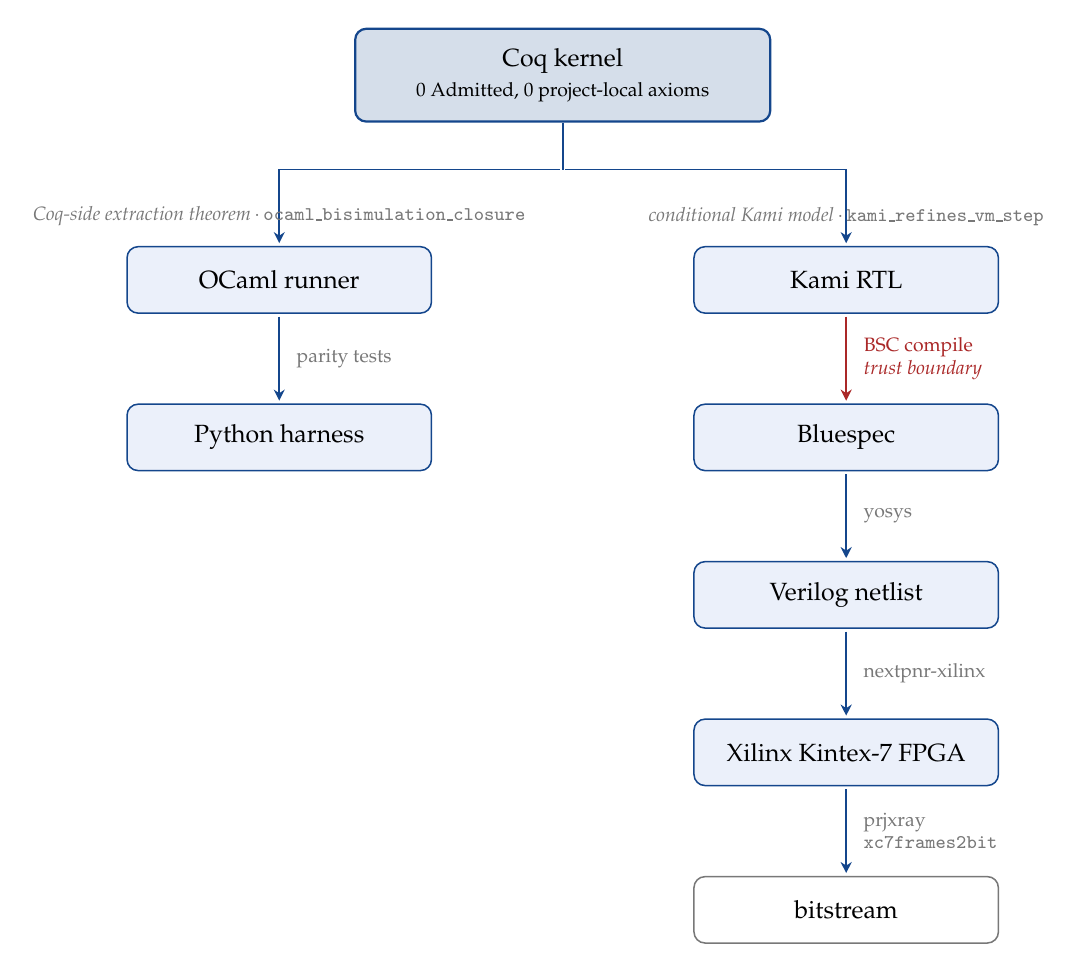
\begin{tikzpicture}[thiele]
\tikzset{
  hbox/.style={
    draw=thiele@accent, line width=0.55pt,
    rounded corners=4pt,
    fill=thiele@pale,
    inner sep=7pt,
    align=center,
    font=\small,
    minimum width=11em,
    minimum height=2.4em
  },
  topbox/.style={
    hbox, fill=thiele@accent!18, line width=0.8pt,
    minimum width=15em
  },
  endbox/.style={
    hbox, fill=white, draw=thiele@gray
  },
  hbarrow/.style={
    ->, line width=0.6pt, draw=thiele@accent,
    shorten >=1pt, shorten <=1pt
  },
  htarrow/.style={
    ->, line width=0.75pt, draw=thiele@red,
    shorten >=1pt, shorten <=1pt
  },
  branchlabel/.style={
    font=\scriptsize, text=thiele@gray, align=center,
    inner sep=2pt
  },
  edgelabel/.style={
    font=\scriptsize, text=thiele@gray, align=left,
    inner sep=2pt
  }
}
% Coq kernel at top center
\node[topbox] (coq) at (0, 6.6)
  {Coq kernel\\\textnormal{\scriptsize 0 Admitted, 0 project-local axioms}};

% Junction point below Coq for the fork
\coordinate (fork) at (0, 5.4);
\draw[line width=0.6pt, draw=thiele@accent] (coq.south) -- (fork);

% Left branch (extraction path)
\node[hbox] (ocaml) at (-3.6, 4.0) {OCaml runner};
\node[hbox] (py)    at (-3.6, 2.0) {Python harness};

% Right branch (silicon path)
\node[hbox] (kami) at (3.6, 4.0) {Kami RTL};
\node[hbox] (bsv)  at (3.6, 2.0) {Bluespec};
\node[hbox] (vlog) at (3.6, 0.0) {Verilog netlist};
\node[hbox] (fpga) at (3.6,-2.0) {Xilinx Kintex-7 FPGA};
\node[endbox] (bit) at (3.6,-4.0) {bitstream};

% Fork arrows: vertical drop, then horizontal to top of each box, then short vertical into box
\draw[hbarrow] (fork) -| (ocaml.north);
\draw[hbarrow] (fork) -| (kami.north);

% Branch labels positioned above the OCaml/Kami boxes, away from arrows
\node[branchlabel, above=0.5em of ocaml.north]
  {\textit{Coq-side extraction theorem}\,$\cdot$\,\code{ocaml\_bisimulation\_closure}};
\node[branchlabel, above=0.5em of kami.north]
  {\textit{conditional Kami model}\,$\cdot$\,\code{kami\_refines\_vm\_step}};

% Left side arrows
\draw[hbarrow] (ocaml.south) -- node[edgelabel, right=4pt]
  {parity tests} (py.north);

% Right side arrows (silicon path)
\draw[htarrow] (kami.south) -- node[edgelabel, right=4pt, text=thiele@red]
  {BSC compile\\\textit{trust boundary}} (bsv.north);
\draw[hbarrow] (bsv.south) -- node[edgelabel, right=4pt]
  {yosys} (vlog.north);
\draw[hbarrow] (vlog.south) -- node[edgelabel, right=4pt]
  {nextpnr-xilinx} (fpga.north);
\draw[hbarrow] (fpga.south) -- node[edgelabel, right=4pt, align=left]
  {prjxray\\\texttt{xc7frames2bit}} (bit.north);

\end{tikzpicture}
\caption{The three-layer realisation. The Coq kernel is the source of truth; the left branch is the runnable-binary path, the right branch is the silicon path. Blue arrows are either conditional Coq-model correspondences (with the theorem named on the edge) or empirical tests. The red and downstream tool arrows are translation/tool trust boundaries unless a separate theorem or artifact says otherwise; no single end-to-end RTL/bitstream bisimulation is claimed.}
\label{fig:hardware-stack}
\end{figure}

\subsection{Layer 1: The Coq kernel}

Coq is where the substrate gets pinned down. The kernel defines:
\begin{itemize}
\item The \texttt{VMState} record (all 12 fields, as in Section~\ref{sec:formal}).
\item The \texttt{vm\_instruction} type: an inductive type (Section~\ref{sec:vocab}) with 51 constructors, one for each opcode, each carrying the right argument types.
\item The \texttt{vm\_apply} function: takes a state and an instruction, returns a state. It is total (Section~\ref{sec:vocab}): every input pair produces a defined output, including the error case.
\item All the theorems: No Free Insight, $\mu$-monotonicity, $\mu$-initiality, categorical separation, Turing strictness, and the rest.
\end{itemize}

The Coq kernel operates mostly over natural numbers, but \texttt{VMState} is not an unbounded mathematical fantasy. \texttt{REG\_COUNT = 16}. \texttt{MEM\_SIZE = 128}. Both are matched against the synthesised RTL. The accessors wrap indices through those sizes (modular arithmetic, Section~\ref{sec:vocab}). Both constants are parametric in the proofs (Section~\ref{sec:vocab}: same proofs, any value), so nothing in the formal chain depends on the specific numbers. Register and memory writes are truncated through the kernel's 64-bit word helpers to keep the math clean. The $\mu$ counter is a plain natural number with no fixed upper bound. The RTL instantiates a finite 32-bit datapath (the part of the chip that moves and operates on data, not the control logic) and bounded tables.

Arithmetic near a word boundary is where a bridge claim can quietly stop meaning what it says, so state it concretely. \texttt{ADD} on the register values $2^{32}-1$ and $1$: 32-bit modular arithmetic wraps the sum to $0$; the kernel's 64-bit word truncation instead gives $2^{32}$, a different value. This is not a hypothetical; it is exactly the gap between the RTL's 32-bit datapath and the kernel's 64-bit word helpers named in the paragraph above. Values whose sum stays under $2^{32}$ agree on both sides; values whose sum crosses that boundary do not, and the bridge domain has to say which side is authoritative for such a value or exclude it. The $\mu$ counter's own range needs the same treatment rather than an unqualified ``unbounded natural on both sides'' reading: the kernel's $\mu$ is a plain unbounded natural number, but the RTL ledger is a fixed-width register, so a program that accumulates enough $\mu$ to exceed that width is outside what the current hardware correspondence establishes, the same way an oversized \texttt{ADD} is.

Zero Admitted means: no step in any theorem proof was asserted without derivation. Coq checked everything. I did not.

\subsection{Layer 2: The OCaml extracted runner}

Here is the trick that makes the OCaml layer worth having at all. A Coq definition is two things wearing one coat: a recipe for computing an answer, and a proof that the recipe behaves. Extraction takes the coat off. It keeps the recipe, in this case rendered into OCaml, an ordinary programming language you can compile and run like any other, and it drops the proof terms on the floor, because a CPU has no use for them. So \texttt{vm\_apply} (the function that defines what every opcode does) walks out the door as an OCaml function that computes the same answer on the same inputs. The proofs do not come along. The algorithm does. That is the whole point: I get a binary I can actually run, descended from the exact definition the theorems were proved about, and the descent is mechanical rather than me retyping the semantics into a second language and praying. The extracted runner executes all 51 opcodes from the Coq semantics, morphism operations and \texttt{CHSH\_LASSERT} included.

The trust boundary at this layer is named explicitly. The kernel proves formal facts about the Coq-side observable (\texttt{shadow\_to\_eo (vm\_apply s i)} strips a state down to its observable fields after one instruction): exact $\mu$ accounting, $\mu$ never decreases, and totality. It also names the external runner boundary. The Coq lemma \code{ocaml\_runner\_agrees} is a reflexive Coq-side boundary marker, not an unproved \texttt{Hypothesis} (Section~\ref{sec:vocab}) and not a cross-language equivalence theorem. The cross-language claim, that the built OCaml binary returns the same observable as the Coq semantics on every input, is checked by the parity test suite (Section~\ref{sec:vocab}: run both on the same battery, verify they agree). I do not count that as a kernel theorem. It is an audited boundary, backed by tests, named in the source.

\subsection{Layer 3: The Kami RTL hardware}

The whole reason this layer exists is to refuse to retype the design in a second language. Kami lets you write a hardware specification inside Coq itself and then extract it, the same move the OCaml runner used, except the target is not software, it is a chip. The first stop is Bluespec SystemVerilog, a hardware description language pitched high enough that you say what the hardware should compute rather than which wire goes where: the registers it holds, the rules it runs, and the conditions under which each state transition is allowed to fire. The Bluespec compiler then drops a level and emits standard Verilog RTL, the gate-and-register description that synthesis tools chew into actual logic, either on an FPGA, a chip you can reconfigure after it leaves the factory, or an ASIC, a chip burned for one design and never reprogrammable. So a Kami module is the same idea descending one more flight of stairs: the finite hardware realisation, pinned down in Coq, walks all the way to gates without anyone hand-translating it on the way, and the Kami extractor runs it through the pipeline above.

The hardware has:
\begin{itemize}
\item $16$ registers, each $32$ bits wide (\texttt{RegCount = 16}; kernel proofs parametric)
\item $128$-bit instruction encoding (\texttt{InstrSz = 128})
\item $128$ words of data memory and $128$ instruction words (\texttt{MemSize = 128}; kernel proofs parametric in \texttt{MEM\_SIZE})
\item bounded instruction transport and execution state
\item $64$ partition module slots (\texttt{PTableSz = 64})
\item $16$ slots in each of the morphism, coupling, formula, certificate, descriptor-metadata, and coupling-pair tables
\item An on-chip \texttt{LASSERT} FSM for formula verification (with $64$-entry inlined backing buffers)
\item The $\mu$ ledger updated atomically with each executed instruction (no separate parallel datapath; the cost arithmetic happens inside the same \texttt{step} rule)
\end{itemize}

The Verilog is the hardware artifact. The FPGA is whatever I could put it on for free. The current target is the Xilinx Kintex-7 \texttt{xc7k325tffg900-2} on the Digilent Genesys~2: the smallest fully-open-toolchain part the design still fits comfortably after the multi-cycle \texttt{CHSH\_LASSERT} witness checker landed. Section~\ref{sec:vocab} explains the synthesis pipeline I use: yosys does the gate-level synthesis, nextpnr-xilinx does the place-and-route, and prjxray's \texttt{xc7frames2bit} produces the bitstream the chip reads to configure itself.

The CI (Full) workflow defines synthesis, simulation, and FPGA-generation jobs.
Resource, timing, and bitstream reports are valid only for the RTL and tool
versions recorded with them. Coq proof compilation does not measure changed
RTL. Current physical claims require regenerated pipeline artifacts linked to
the source identity in Section~\ref{sec:reproduction}.

The kernel proofs are parametric in \texttt{REG\_COUNT} and \texttt{MEM\_SIZE}, so the same proofs apply at any size constants the design picks. This part was a proof of existence on hardware, not a design constraint. The size constants (16 registers, 128 data words, 128 instruction words) were chosen small enough to fit on a free-toolchain FPGA. The design scales to whatever size you actually want.

47 of the 51 opcodes are implemented in the synthesized RTL: the Kami core has hardware logic for those 47, and the synthesised Verilog carries them through to the FPGA bitstream. The remaining four (the Q\textsubscript{1+AB} check-opcode family \code{instr\_chsh\_lassert\_1ab}, \code{instr\_chsh\_lassert\_1ab\_g5}, \code{instr\_chsh\_lassert\_1ab\_g345}, \code{instr\_chsh\_lassert\_1ab\_g12345}) are defined in the Kami HW abstraction with kernel-equivalence proven, and they execute in the OCaml runner and Python harness, but they are not synthesized into the FPGA bitstream because the synthesized design already fills most of the chip and each of them would need its own wide-arithmetic FSM. The OCaml/RTL opcode-set parity test tolerates exactly these four. The question is not which opcodes are in hardware, but which opcodes have a completed formal \emph{bisimulation proof}.

The theorem \code{KamiHW.GraphReconstructionBridge.driven\_step\_wf} compares the Gallina function \texttt{kami\_step} with \texttt{Kernel.SimulationProof.vm\_apply} through \texttt{abs\_full\_snapshot}. Its premise is \texttt{WFDrivenPrecondition ks i}. The trace theorem \texttt{driven\_trace\_commutes} requires \texttt{WFDrivenRun fuel trace ks}, which checks that premise at every visited state. This is the intermediate Coq model surface, separate from physical clock transitions in \texttt{ThieleCPUCore.v}.

\begin{itemize}
\item The default branch of \texttt{WFDrivenPrecondition} is \texttt{True}. It adds no instruction-specific premise to this intermediate model equality.
\item CALL and RET require \texttt{WellFormedSnapshot}, with a PC bound for CALL. CHSH\_TRIAL requires Boolean operands. LASSERT requires agreement with its memory header. Tensor access requires valid indices, and TENSOR\_GET also requires module existence.
\item MORPH requires \texttt{extended\_hw\_invariant} and existing source and target modules. COMPOSE, MORPH\_TENSOR, and MORPH\_GET require the extended invariant. MORPH\_ID uses the empty-descriptor invariant and module existence. MORPH\_ASSERT and MORPH\_DELETE require morph-table well-formedness.
\item PNEW requires a nonempty normalized region and fresh tensor state. PSPLIT and PMERGE carry the partition, capacity, freshness, and arithmetic conditions in their source branches. These per-operation conditions must be established along the actual run; reset alone does not provide unlimited table capacity.
\end{itemize}

The actual CPU rules also have executable Kami semantics. \code{CoreRules} places all twelve rules in the supported linear-action fragment; \code{CoreExecution} proves that finite traces of its first-enabled selector are actual Kami multi-step executions, with a firing bound and an early-stop characterization by absence of enabled rules. Reset has an enabled selected rule. \code{CoreTyping} proves preservation of the complete register-name/kind schema from reset, while \code{DispatchReset} states thirteen typed initialization facts. These results establish selected execution and register types. They do not establish fairness, reachable allocation/resource invariants, the full abstract observation relation, or semantic preservation through the RTL toolchain.

Finite RTL transfer additionally requires compatible word ranges, memory addressing, allocation capacity, reset state, and observation at instruction retirement. For example, adding $2^{32}-1$ and 1 yields zero in a 32-bit register and $2^{32}$ in the kernel's 64-bit arithmetic. Exact numerical equality therefore needs a range restriction or an explicitly proved modular abstraction. The finite ledger similarly needs a no-overflow bound for exact natural-number equality. Multi-cycle operations require a retirement relation that accounts for intermediate FSM states.

The coupling FSM reads serialized MORPH pairs and implements pair copying and relational joins for the other two operations. Descriptor zero remains reserved for empty/identity couplings. The finite pair table holds 16 entries; insufficient space raises an error, and empty results need no pair entries. The RTL regression tests inspect the backing pair tables through the testbench. They do not establish full-state refinement: hardware lacks the software coupling-label field and module-membership filter, and the full endpoint/region representation contract remains an obligation for a broader physical correspondence claim. The RTL normalizes the newly allocated pair range, retaining each pair's last occurrence as the software's \texttt{nodup} does. Allocation first requires room for the raw intermediate list; a normalized result fitting the table does not guarantee admission when the raw list exceeds it.

The inventory arithmetic \texttt{rtl\_coverage\_partition} is not a proof of these representation obligations. The 47 synthesized / four nonsynthesized distinction describes the implementation inventory; it does not turn a conditional model theorem into unrestricted RTL equality.

And the four Q\textsubscript{1+AB} check opcodes are not stranded by sitting outside that partition: their kernel-equivalence proof makes them sound at the substrate level (see \S\ref{sec:chsh}), and they run in the OCaml runner and Python harness. What they lack is a synthesized-Verilog counterpart to bisimulate against, which is why they fall outside the 47 rather than inside it as a gap. That is honest proof accounting, not a hole papered over.

The substrate is the math. The Coq kernel pins it down. The hardware is a finite physical instantiation with explicit table sizes and word widths. The proofs state the bridge between them under the finite representation invariants where those invariants are needed. This is the only honest relationship physical hardware can have with an abstract mathematical substrate.

\medskip
\noindent\textbf{Substrate-level vs program-level enforcement.} In the Coq kernel, A2 is part of the step relation. A2 says: flipping certification false-to-true costs at least 1, at the step level. Look at the cases for \texttt{CERTIFY} and \texttt{MORPH\_ASSERT} in \texttt{vm\_apply}: the cost is added before the flag flips; the step that mutates the certification channel and the step that charges $\mu$ are the same step. That is what A2 means in the kernel.

A correct conventional simulator can preserve the VM invariant on its encoded states. A different or buggy simulator may fail to do so; that does not establish an incapacity theorem about conventional computation. The VM theorem constrains its own transition relation. Hardware transfer additionally requires the representation conditions of \texttt{WFDrivenRun} and the documented extraction and compiler trust boundaries.

Enforcement, representation, and observation must be assessed separately. The abstract A2 theorem allows arbitrary state types and designated predicates. Exact unit pricing is a stronger condition relative to certification-flip count; A2 itself permits larger charges. Neither result authenticates an external receipt without an evidence interface.

%===========================================================================
\section{Five minimal models inspired by other disciplines}
\label{sec:reductions}
%===========================================================================

The abstract records leave state and instruction types open. The following five examples instantiate them with deliberately minimal models inspired by independently developed disciplines. Coq checks the models and their consequences; correspondence with deployed protocols remains a modeling claim requiring separate evidence.

\subsection{Proof-of-stake finality}

The formal finality example uses a Boolean finalized flag and a nonnegative stake-at-risk charge on a finalizing transition. A zero-charge transition from unfinalized to finalized violates its A2 obligation. A schedule charging at least one unit on that transition satisfies the obligation. This model records exposure to loss. It does not assert that collateral was actually destroyed, that successive exposures are distinct spent units, or that every deployed consensus protocol uses this mechanism.

In this model, \code{nothing\_at\_stake\_is\_free\_forgery} excludes an A2 instance for the supplied free-finalization witness. Under the slashing-schedule premise, \code{slashing\_finality\_floor} bounds the sum of modeled charges along an initially unfinalized, finally finalized run by at least one. Applying this result to a deployed protocol requires a correspondence between its transitions and the model.

Falsifier: a transition system satisfying the stated slashing-schedule and execution premises with an initially unfinalized, finally finalized trace whose modeled charge sum is zero.

\subsection{Gas metering}

The gas example defines a unit commitment counter. \code{gas\_schedule\_exactness} gives a biconditional characterization of exact pricing relative to its designated commitment predicate: floor and no-overcharge together identify the charging predicate and unit price, and the exactness conclusion implies those conditions back. A deployed gas schedule also prices resources such as computation and storage. Its full fee is not identified with this counter.

The model separates missing mandatory charges from overcharging the reference counter. \code{undercharged\_opcode\_admits\_free\_commitment} concerns a committing step charged zero. \code{overcharge\_breaks\_exactness} concerns the no-overcharge condition. The VM has an exact state-dependent commitment pricer, \code{thiele\_vm\_commit\_pricing\_is\_exact}, bounded above by its full ledger schedule via \code{thiele\_unit\_price\_lower\_bounds\_mu}. Repeated CERTIFY instructions illustrate the distinction: each pays the instruction floor, while only a false-to-true transition contributes to the flip counter.

Falsifier: a schedule satisfying floor and no-overcharge whose charging predicate differs from the commitment predicate on some reachable step.

\subsection{Trusted-execution attestation}

The attestation model enriches a report with a measurement field. Under the stated coverage and evidence assumptions, \code{attestation\_cannot\_factor\_through\_bare\_transcript} excludes a sound and complete verifier using only the specified bare transcript. \code{replay\_is\_a\_two\_preimage\_witness} supplies the model's collision, and \code{measurement\_enriched\_attestation\_succeeds} supplies a verifier for its enriched reports. This construction requires distinguishing evidence. It does not force a particular physical register or authenticate an adversarially supplied measurement.

Falsifier: a sound and complete attestation scheme for a $\mu$-dependent claim that reads only the bare transcript.

\subsection{Certificate transparency}

The transparency example supplies a log-like evidence field within the hardness escape model. \code{transparency\_log\_escape} inherits that model's acceptance guarantee and trust assumptions. \code{log\_free\_verifier\_impossible} excludes the specified bare verifier under the collision and coverage premises. \code{split\_view\_witness} is a pair in this model. Identifying these fields with a deployed certificate-transparency protocol requires a separate implementation and security argument.

Falsifier: a sound and complete log-free verifier with the same soundness target.

\subsection{Proof-carrying verification}

The proof-carrying example supplies evidence in a transcript field called rounds. \code{proof\_rounds\_escape} verifies that field under its evidence contract; \code{bare\_pcc\_impossible} concerns removing the distinguishing evidence. A noninteractive certificate does not become an interactive protocol because of this field name. Separately, \code{level\_k\_verification\_floor} bounds the modeled cost of $k$ charged certification events, with a tightness witness in \code{level\_k\_verification\_floor\_tight}. This event count differs from the single-instruction charge levels in Section~\ref{sec:landauer}. Neither count measures prover time, circuit size, or proof length.

Falsifier: a level-$k$ certified trace with total $\mu$ below $k$, or a sound and complete zero-round bare verifier.

\subsection{The same table, five ways}

\begin{center}
{\small
\begin{tabular}{p{5.2em} p{5.5em} p{8.5em} p{7em} p{8em}}
\textbf{System} & \textbf{Escape used} & \textbf{Kernel result} & \textbf{Model consequence} & \textbf{What refutes it} \\
\hline
PoS finality & none, the cost records directly & \code{universal\_nfi\_any\_substrate} & modeled finalization charge $\geq 1$ & a zero-stake gadget admitting A2 \\
Gas metering & none, a pricing biconditional & \code{exact\_commitment\_pricing\_characterization} & charge $\equiv$ commit, unit price & a conforming non-commitment schedule \\
TEE attestation & substrate (enrich the state) & \code{V\_does\_not\_factor\_through\_classical} & distinguishing evidence & sound+complete bare-transcript attestation \\
Transparency logs & hardness & \code{hardness\_escape\_succeeds} & the supplied evidence & sound+complete log-free verifier \\
Proof-carrying / ZK & interaction & \code{interactive\_escape\_succeeds}, \code{level\_k\_certification\_cost\_floor} & evidence, and $k$ units for $k$ charged events & a level-$k$ trace under $k$ $\mu$ \\
\end{tabular}
}
\end{center}

These five constructions establish consequences of their explicit records. Deployment interpretations require independent evidence. The examples do not establish that certification is the unique event every model must price; that broader selection question remains open.

%===========================================================================
\section{Binary Game Statistics: where the \texorpdfstring{$\mu$}{mu}-Ledger Meets the NPA Boundary}
\label{sec:chsh}
%===========================================================================

The substrate has a CHSH step. The VM realises it with two opcodes. \texttt{CHSH\_TRIAL} records outcomes of a 2-player binary game into hardware witness counters. \texttt{CHSH\_LASSERT} refuses to advance normally unless those counters satisfy a Z-arithmetic check.

The enforcement doesn't care who built the wall. \texttt{CHSH\_LASSERT} refuses a super-quantum correlation by trapping to \texttt{LASSERT\_TRAP\_PC}; \texttt{LASSERT} refuses a formula whose dual witness fails to exclude a single valuation by trapping to the same address, the same way. One wall is the Tsirelson bound, which I did not author and could not have. The other is a logical constraint I wrote down myself. The step traps the same on both. So $\mu$ isn't pricing contact with external structure as some special case. It prices the certified narrowing as such, and the trap fires the same whether the state it throws out is a PR box or a falsifying assignment I handed it. Insight costs, and the price never asks whether you found the wall or built it.

And the claim is about that step, not the chip. Some of these cert-opcodes never reach the synthesised FPGA. That's a silicon budget, not a hole in the argument: the trap is the cost-on-certification law, and the law lives in the transition, not the gate count.

Everything below earns that. The matrix algebra is the discharge: it shows the wall \texttt{CHSH\_LASSERT} traps against is real and externally fixed, the Tsirelson boundary, not a bar I set myself. I came at it sideways, stress-testing the $\mu$-ledger's cost algebra against a known algebraic boundary, the NPA moment matrix conditions for what correlations are achievable under polynomial constraints.

I did not set out to find what I found. The chain is concrete. The Z-arithmetic check the kernel runs on the witness counters (decidable, integer-only) is sound with respect to the real-valued column-contractive predicate by \code{column\_contractive\_check\_witness\_sound} (188 lines, closing with \texttt{nra} after IZR distribution and field simplification). That real-valued predicate is biconditional with PSD of the specified zero-marginal, zero-within-party-moment matrix by \code{column\_contractive\_iff\_quantum\_realizable}. End-to-end: a successful \texttt{CHSH\_LASSERT} step entails PSD of that specified matrix on the witness-derived correlators, by \code{chsh\_lassert\_no\_trap\_implies\_quantum\_realizable}. No quantum-mechanical premises live in the Coq dependency tree: no Hilbert space, no operators, no observables. The identification of that PSD condition with quantum-realizable correlations lives in the NPA framework itself (Navascu\'es--Pironio--Ac\'in 2007, 2008). I cite it. I do not derive it. The kernel's content is the algebraic bridge between an integer-arithmetic check inside an opcode and PSD of a specific matrix. The name ``quantum-realizable'' in the source is borrowed from that literature, not earned by a physics derivation inside the kernel.

\medskip
\noindent\textbf{Direction of derivation: substrate first, NPA second.}
Two passes, in this order. First pass, substrate-side: the \texttt{CHSH\_TRIAL} opcode, its witness-counter cost schedule, the integer Z-arithmetic predicate \code{column\_contractive\_check} that \texttt{CHSH\_LASSERT} runs on those counters, and the soundness of that integer check against its real-valued lift. None of this references NPA. The coherence condition the $\mu$-ledger enforces at \texttt{CHSH\_LASSERT} is: a successful witness check requires the counters to satisfy three explicit polynomial inequalities on cleared integer ratios. That predicate is defined inside the cost algebra and verified by the kernel without consulting the quantum-mechanics literature. Second pass: formal matrix agreement. The substrate-native predicate, lifted to the reals via IZR and the witness-count denominators, is the column-contractive predicate; the column-contractive predicate is biconditional with PSD of the specified zero-marginal, zero-within-party-moment matrix. The biconditional compares two explicitly defined mathematical predicates, proven in pure polynomial arithmetic with no project-local axioms. It is not a theorem that the runtime has constructed a physical quantum experiment. The load-bearing result is §\ref{sec:chsh}'s ``Algebraic characterization of the $\mu$-ledger gate condition'' subsection. The earlier subsections (Bell test setup, classical bound, quantum bound) are the walk there. If you have time for one subsection, that is the one. The CHSH game is built from scratch in the next subsection so the result makes sense to readers who have not seen Bell tests before; readers who have can skip ahead.

\subsection{The Bell test setup, from scratch}

Imagine two players, Alice and Bob, in separate rooms. They cannot communicate once the game starts. A referee sends Alice one of two questions ($x \in \{0,1\}$). The referee sends Bob one of two questions ($y \in \{0,1\}$). Alice answers $a \in \{0,1\}$. Bob answers $b \in \{0,1\}$. (Settings $(x,y)$, outcomes $(a,b)$: same convention as Section~\ref{sec:formal} and the Coq.)

The game rule: they want $a \oplus b = x \land y$. The symbol $\oplus$ is XOR (exclusive OR): $a \oplus b = 1$ when $a \neq b$, and $0$ when $a = b$. The symbol $\land$ is AND: $x \land y = 1$ only when both $x = 1$ and $y = 1$, otherwise 0. In plain language: their answers should be different if and only if both questions were 1. For all other question combinations (both 0, or one each), they should match.

\begin{figure}[!htbp]
\centering
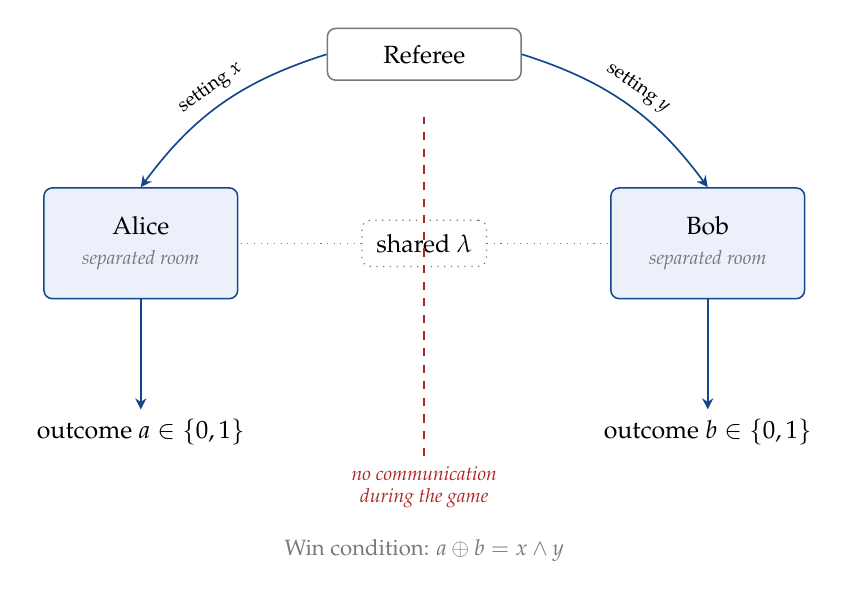
\begin{tikzpicture}[thiele]
% Referee at top
\node[
  draw=thiele@gray, line width=0.55pt,
  rounded corners=3pt,
  fill=white,
  inner sep=6pt,
  font=\small,
  minimum width=7em
] (ref) at (0, 2.4) {Referee};

% Alice on the left
\node[
  draw=thiele@accent, line width=0.55pt,
  rounded corners=3pt,
  fill=thiele@pale,
  inner sep=8pt,
  align=center,
  font=\small,
  minimum width=7em,
  minimum height=4.0em
] (alice) at (-3.6, 0) {Alice\\\scriptsize\itshape\color{thiele@gray} separated room};

% Bob on the right
\node[
  draw=thiele@accent, line width=0.55pt,
  rounded corners=3pt,
  fill=thiele@pale,
  inner sep=8pt,
  align=center,
  font=\small,
  minimum width=7em,
  minimum height=4.0em
] (bob) at (3.6, 0) {Bob\\\scriptsize\itshape\color{thiele@gray} separated room};

% Shared randomness lambda
\node[
  draw=thiele@gray, line width=0.45pt,
  dotted,
  rounded corners=3pt,
  fill=white,
  inner sep=5pt,
  font=\small,
  minimum width=4.5em
] (lambda) at (0, 0) {shared $\lambda$};

% Outputs at the bottom
\node[font=\small] (aout) at (-3.6, -2.4) {outcome $a \in \{0,1\}$};
\node[font=\small] (bout) at ( 3.6, -2.4) {outcome $b \in \{0,1\}$};

% Referee delivers settings
\draw[pipearrow] (ref.west) to[bend right=18]
  node[above, font=\scriptsize, sloped] {setting $x$} (alice.north);
\draw[pipearrow] (ref.east) to[bend left=18]
  node[above, font=\scriptsize, sloped] {setting $y$} (bob.north);

% Lambda links to both players (agreed beforehand)
\draw[line width=0.4pt, dotted, draw=thiele@gray]
  (lambda.west) -- (alice.east);
\draw[line width=0.4pt, dotted, draw=thiele@gray]
  (lambda.east) -- (bob.west);

% Alice and Bob produce outputs
\draw[pipearrow] (alice.south) -- (aout);
\draw[pipearrow] (bob.south) -- (bout);

% No-comm barrier line
\draw[line width=0.6pt, dashed, draw=thiele@red]
  (0, -2.7) -- (0, 1.6);
\node[font=\scriptsize\itshape, text=thiele@red, align=center]
  at (0, -3.1) {no communication\\during the game};

% Game-rule annotation
\node[font=\footnotesize, text=thiele@gray, align=center]
  at (0, -3.9) {Win condition: $a \oplus b = x \land y$};

\end{tikzpicture}
\caption{The CHSH setup. The referee distributes settings $x,y$; Alice and Bob each have a separated room and may share an agreed-on $\lambda$ from before the game started. No communication during the game. Each produces a binary outcome ($0/1$ on the wire, recoded as $\pm 1$ for the correlators). The four correlators $E_{xy} = \langle a b\rangle$, read in the $\pm 1$ encoding, are what the kernel's CHSH\_LASSERT instruction checks against the column-contractivity / NPA condition.}
\label{fig:chsh-setup}
\end{figure}

\medskip
\noindent\textbf{Why 75\% is the classical ceiling.}
Before the game, Alice and Bob can agree on any deterministic strategy: a function $a(x, \lambda)$ for Alice and $b(y, \lambda)$ for Bob, where $\lambda$ is any shared randomness they agree on in advance. Once the game starts, no communication. One assumption, said out loud: the referee asks the four question pairs equally often. That is where the 75\% comes from. Drop it and the exact statement is only that every deterministic strategy loses at least one of the four pairs.

Fix any deterministic strategy and freeze $\lambda$. Then Alice has two predetermined answers, $a_0$ and $a_1$, and Bob has two predetermined answers, $b_0$ and $b_1$. Winning all four question combinations would require:

\[
a_0 \oplus b_0 = 0,\quad
a_0 \oplus b_1 = 0,\quad
a_1 \oplus b_0 = 0,\quad
a_1 \oplus b_1 = 1.
\]

Now XOR the four left sides. Every variable appears twice, so the total is 0. XOR the four right sides and the total is 1. That is impossible. So every deterministic local strategy loses at least one of the four cases, and the best deterministic strategy wins at most 3 out of 4 question combinations.

And you cannot buy your way past it with a coin flip. A randomized strategy is nothing but a bag of deterministic ones with a die deciding which to pull, and every strategy in the bag already tops out at 75\%. Average a pile of things that each sit at 75\% or below and the average sits at 75\% or below; there is no arrangement of losers that sums to a winner. That is linearity of expectation, the most boring theorem in the building, quietly closing the last door.

So under that uniform-setting contract the classical ceiling is 3/4, seventy-five percent, and not a hair more. And I do not want you to take that on the strength of an XOR trick on a page; the reference kernel pins it down both ways and leaves nothing Admitted. One executable trace, built from nothing but \texttt{PNEW}, \texttt{PSPLIT}, and \texttt{CHSH\_TRIAL} and never spending a cent of the cost ledger ($\mu = 0$), walks right up to 75\% and touches it. Then \code{local\_box\_CHSH\_bound} closes the lid from the other side: no local strategy, however randomized, no factorizable box anywhere, gets over the line under the stated population/setting-weight assumptions. A trace can of course just \emph{write} any tallies it likes into the counters at $\mu = 0$, the way anyone can write a fake scoreboard; the theorem is about what local play can earn, and the certification step that would stand behind a scoreboard is the priced one. The achievable and the unbeatable land on the same number, which is the only kind of ceiling I trust.

\subsection{The CHSH inequality: where it comes from}

Now here is what took me a while to understand: why is there a specific algebraic combination $S$ that detects whether correlations can be explained classically?

The key move is this. For any fixed shared randomness $\lambda$, Alice's output $A_x(\lambda) \in \{-1, +1\}$ (I'm using $\pm 1$ encoding now, not $0/1$, indexed by Alice's setting $x$) and Bob's $B_y(\lambda) \in \{-1, +1\}$ (indexed by Bob's setting $y$). Consider the expression:

\[
A_0(\lambda) B_0(\lambda) + A_0(\lambda) B_1(\lambda) + A_1(\lambda) B_0(\lambda) - A_1(\lambda) B_1(\lambda)
\]

Factor it:

\[
= A_0(\lambda)(B_0(\lambda) + B_1(\lambda)) + A_1(\lambda)(B_0(\lambda) - B_1(\lambda))
\]

Since $B_0$ and $B_1$ are each $\pm 1$, either $B_0 + B_1 = \pm 2$ and $B_0 - B_1 = 0$, or $B_0 + B_1 = 0$ and $B_0 - B_1 = \pm 2$. The two terms cannot both be large. In either case, $|B_0 + B_1| + |B_0 - B_1| = 2$, and since $|A_0|, |A_1| \leq 1$, the entire expression is at most 2 in absolute value for any fixed $\lambda$.

Average over $\lambda$:

\[
S = \langle A_0 B_0 \rangle + \langle A_0 B_1 \rangle + \langle A_1 B_0 \rangle - \langle A_1 B_1 \rangle
\]

where $\langle A_x B_y \rangle$ is the correlation (expected value of the product) when settings are $x$ and $y$. Since the expression before averaging was bounded by 2 for every $\lambda$, the average satisfies $|S| \leq 2$.

That is the argument. The combination with the minus sign is chosen exactly because the factoring trick works: one of the B-terms goes to zero and the other to $\pm 2$, forcing the whole thing below 2. The inequality $|S| \leq 2$ is a pure algebraic consequence of the outputs being $\pm 1$ and being determined locally.

None of that lives only in my head. The argument I just walked you through is the English proof; the formal check that I did not fool myself anywhere is \code{local\_box\_CHSH\_bound}, which says the plain thing in symbols: for any factorizable box B, $|S(B)| \leq 2$, with nothing left Admitted. And a bound from above is only half an honest claim. \code{classical\_bound\_achieved} hands over the other half, a constructive witness, an executable trace at $\mu = 0$ that actually reaches $|S| = 2$ rather than just respecting it. Put the two together and the ceiling is not loose: $\max\{|S| : B\ \text{factorizable}\} = 2$, exactly, no slack to argue about, and a $\mu = 0$ trace reaches it.

\subsection{\texorpdfstring{The quantum bound: why $2\sqrt{2}$?}{The quantum bound: why 2 sqrt 2?}}

Now hand the same game to quantum mechanics and the ceiling lifts. Not to anything you please, and not all the way to a perfect 4; it lifts to $2\sqrt{2} \approx 2.828$ and stops there as hard as the classical 2 stopped. That number is the Tsirelson bound, named for Boris Tsirelson, who was the first to write down $|S| \leq 2\sqrt{2}$ and pin quantum correlations under it. The physics story of \emph{why} it is that exact number, and not some other irrational nobody would have guessed, runs through Hilbert-space operators, anticommutators, the Pauli matrices, the Bloch sphere, the whole machinery. It is a real and beautiful derivation and I am going to walk straight past it, because none of the formal content here leans on it. I do not need to retell quantum mechanics to show you the kernel respects the wall; I only need the algebra, and that is what I am keeping.

What the formal content does depend on, and what I will derive in the next subsections, is the algebra. One bridge theorem is parameterized by the predicate named ``quantum-realizable in the zero-marginal NPA framework''; that name records the external NPA interpretation and is a premise, not a physical derivation in Coq. Its conclusion is the algebraic bound $|S| \leq 2\sqrt{2}$. The ``What the cost algebra proves'' subsection below then builds the same bound from polynomial inequalities on the specified moment matrix without any quantum-physics premise at all. That is the path I follow, and the formal claim is the algebraic one.

And that gap between 2 and $2\sqrt{2}$ is not bookkeeping. It is the most stubborn fact in physics: people have gone into labs, fired entangled photons through polarizers, counted coincidences, and watched the number sit up above 2 where no local classical story is allowed to put it. Whatever the world is doing, it is not Alice and Bob with a shared cheat sheet agreed beforehand. The physics of \emph{why} the wall sits at $2\sqrt{2}$ is somebody else's chapter and a good one. My question is narrower and, to me, stranger: why does the kernel's CHSH check respect a wall it was never told about? The polynomial arithmetic below answers it. Feed the cost ledger nothing but its own algebra, no quantum mechanics anywhere in the room, and the same $2\sqrt{2}$ falls out the bottom on its own.

\medskip
\textbf{A note on the rational approximation in the kernel.} The kernel names the rational threshold $5657/2000 \approx 2.8285$ for exact rational comparisons (you can verify $(5657/2000)^2 = 32{,}001{,}649 / 4{,}000{,}000 > 8$, so $5657/2000 > \sqrt{8} = 2\sqrt{2}$). The real-valued quantum-model bridge uses $\sqrt{8}$ directly. Those are two different proof surfaces, and I keep them apart on purpose: the rational one so a machine can check it in exact arithmetic, the real one so the quantum bridge has something to bite on.

\subsection{What the cost algebra proves}

\begin{theorem}[Classical CHSH Bound]
For population correlations with a setting-independent shared-variable distribution, Alice's local response depending on $x,\lambda$ and Bob's on $y,\lambda$, $|S|\leq2$. The constant strategy attains equality. Its four-setting VM witness has zero charge when every trial uses $\delta=0$.
\end{theorem}

\begin{proof}
$|S| \leq 2$: the XOR-factoring argument from Section~\ref{sec:chsh}'s ``Why 75\% is the classical ceiling.'' Fix any local deterministic strategy and any $\lambda$. Alice produces $A_x(\lambda) \in \{-1, +1\}$; Bob produces $B_y(\lambda) \in \{-1, +1\}$. The quantity
\begin{multline*}
A_0(\lambda) B_0(\lambda) + A_0(\lambda) B_1(\lambda) + A_1(\lambda) B_0(\lambda) - A_1(\lambda) B_1(\lambda) \\
{} = A_0(\lambda)(B_0(\lambda) + B_1(\lambda)) + A_1(\lambda)(B_0(\lambda) - B_1(\lambda))
\end{multline*}
satisfies $|\cdot| \leq |B_0 + B_1| + |B_0 - B_1| = 2$ (because for $B_0, B_1 \in \{\pm 1\}$, one of $|B_0 + B_1|$ and $|B_0 - B_1|$ is $2$ and the other is $0$, and $|A_0|, |A_1| \leq 1$). Average over $\lambda$ to get $|S| \leq 2$. Mixtures of deterministic strategies are convex combinations, so the same bound holds by linearity of expectation.

Tightness: the strategy $A_x \equiv 1$, $B_y \equiv 1$ gives $\langle A_0 B_0 \rangle = \langle A_0 B_1 \rangle = \langle A_1 B_0 \rangle = \langle A_1 B_1 \rangle = 1$, so $S = 1 + 1 + 1 - 1 = 2$. This is achievable at $\mu = 0$ by a program with all $\delta = 0$ instructions accumulating one trial per setting pair in \texttt{vm\_witness}. The Coq witness is \code{classical\_bound\_achieved}. \qed
\end{proof}

\begin{plainreading}
Factor the expression. Two terms. One has $B_0 + B_1$, the other has $B_0 - B_1$. With $B_0, B_1 \in \{\pm 1\}$, only one can be nonzero at a time, and the nonzero one is $\pm 2$. Multiply by $|A| \leq 1$. The whole expression caps at 2. Average over $\lambda$, you get $|S| \leq 2$. To make it 2, just have both players always answer 1.
\end{plainreading}

\begin{theorem}[Non-locality of an exact CHSH violation]
An exact correlation $\mathbf{E} = (E_{00}, E_{01}, E_{10}, E_{11})$, with $S = E_{00} + E_{01} + E_{10} - E_{11}$ and $S > 2$, cannot arise as the population-level correlation of any local hidden variable model (the term is built in Section~\ref{sec:vocab}: a classical-physics-style theory where outcomes come from shared randomness $\lambda$ plus local settings). This is a claim about the idealized correlator, the value an unbounded run of trials at each setting converges to. It is not yet a claim about any one finite tally of recorded trials; that distinction is spelled out below.
\end{theorem}

\begin{proof}
Contrapositive of the Classical CHSH Bound. Any LHV model produces a locally factorizable correlation by definition: each player's outcome is a function of their setting and the shared $\lambda$. The theorem above says all such correlations satisfy $|S| \leq 2$. So an idealized correlation with $S > 2$ cannot have arisen from any LHV model. \qed
\end{proof}

\begin{plainreading}
Direct contrapositive. If $|S| \leq 2$ for the population-level correlation of every LHV, then a population-level $S > 2$ rules out every LHV. The Bell-test contradiction is in this form, and it is a claim about the number an unbounded run converges to, not the number on any one finite scoreboard.
\end{plainreading}

\begin{remark}
\textbf{A finite scoreboard is not the population correlation.} A \texttt{WitnessCounts} tally from a finite run of \texttt{CHSH\_TRIAL} instructions is a sample statistic, \code{chsh\_stat\_from\_wc}, not the idealized correlator the theorem above bounds. A local hidden variable model can draw a fresh $\lambda$ per trial, and a short run can land away from its own population mean by chance. Run one trial at each of the four settings, with Alice and Bob each answering an independent fair coin flip, an honest LHV strategy with population correlation zero at every setting: the event ``same at $(0,0)$, same at $(0,1)$, same at $(1,0)$, different at $(1,1)$'' has probability $1/16$ and produces the finite tally $S = 4$, the algebraic maximum, with no communication and no quantum content anywhere in the construction. This is the same finite-sample distinction Zhang, Glancy, and Knill work out in full for Bell tests (\emph{Efficient quantification of experimental evidence against local realism}, arXiv:1303.7464): a population bound of $|S| \leq 2$ is not, by itself, a claim that every finite sample drawn from a local model also satisfies it.

What the kernel proves about a finite tally is narrower, and it does hold: \code{chsh\_violation\_rules\_out\_locally\_factorizable\_coupling} shows that a tally with $S > 2$ is inconsistent with any single fixed deterministic strategy $(a_0, a_1, b_0, b_1)$ replayed identically at every recorded trial (\code{locally\_consistent\_classical\_bound} is the converse direction: a tally consistent with one fixed deterministic strategy has $|S| \leq 2$). That rules out one specific, narrow explanation of the tally. It does not rule out a randomized local model that redraws $\lambda$ trial by trial, which is exactly the kind of model the coin-flip example above uses to reach $S = 4$ honestly. Reading a certified witness violation as physically informative rests on running enough trials to make the fixed-strategy count and the population count converge, not on an identity between one finite tally and the exact-correlation theorem above.
\end{remark}

\begin{theorem}[Tsirelson upper bound for the fixed completion]
If the correlators satisfy PSD of the specified zero-marginal, zero-within-party-moment completion, their CHSH value satisfies $|S|\leq\sqrt{8}=2\sqrt2$.
\end{theorem}

\begin{proof}
The fixed-matrix biconditional gives column contractivity. It bounds each row norm of $E$ by one. Apply Cauchy--Schwarz to $S=(E_{00}+E_{01})+(E_{10}-E_{11})$: each parenthesis has magnitude at most $\sqrt2$ times its row norm. Thus $|S|\leq2\sqrt2$. This proof uses the specified matrix, without an identification with arbitrary zero-marginal operator models. \qed
\end{proof}

\begin{plainreading}
PSD of the fixed matrix and column contractivity are the same condition. Column contractivity caps each row, and Cauchy--Schwarz turns those row caps into $2\sqrt{2}$. That is a statement about this matrix. A quantum behavior in general, or a finite local sample, is a different object with its own definition.
\end{plainreading}

\begin{theorem}[General algebraic Tsirelson bound]
For every real quadruple satisfying the two explicit row constraints
$E_{00}^2+E_{01}^2\leq 1$ and $E_{10}^2+E_{11}^2\leq 1$, the CHSH value satisfies $S^2\leq 8$, that is, $|S|\leq 2\sqrt{2}$. These are the exact hypotheses of \code{tsirelson\_from\_row\_bounds}; the theorem does not quantify over unspecified minor witnesses or hidden parameters $t$ and $s$.
This is an algebraic statement about four real numbers, not a completeness theorem for quantum behaviors. The Coq proof uses the explicit six-square Cauchy--Schwarz identity \code{cauchy\_schwarz\_chsh}, then adds the two row inequalities. The rational approximation corollary uses $5657/2000$ as an exact rational overestimate of $2\sqrt{2}$ (you can verify $(5657/2000)^2 = 32{,}001{,}649 / 4{,}000{,}000 > 8$), allowing the bound to be checked in exact rational arithmetic without floating-point. No physics premises. Pure polynomial arithmetic. The Tsirelson bound $2\sqrt{2}$ is derived from algebra, not assumed.
\end{theorem}

\begin{proof}
The proof has two rows, not four unspecified $3 \times 3$-minor constraints. First add the two row inequalities to obtain $E_{00}^2+E_{01}^2+E_{10}^2+E_{11}^2\leq2$. Then \code{cauchy\_schwarz\_chsh} gives the explicit identity
$4\sum E_{xy}^2-S^2\geq0$, a sum of six squares. Combining the two facts yields $S^2\leq8$. No parameters $t,s$ occur in this theorem or its proof.

The rational approximation corollary uses $5657/2000$ in place of $\sqrt{8}$ to keep the comparison in $\mathbb{Q}$: $(5657/2000)^2 = 32{,}001{,}649/4{,}000{,}000 > 8 = 32{,}000{,}000/4{,}000{,}000$, so $5657/2000 > \sqrt{8}$. Combined with $|S|^2 \leq 8$, this gives $|S| < 5657/2000$, a strict rational bound checkable without floating-point evaluation. \qed
\end{proof}

\begin{plainreading}
Two row inequalities, one six-square identity, done. That is the whole proof. No hidden parameters. No physics. The $2\sqrt{2}$ falls out of the algebra; nobody put it in. What the theorem covers is four real numbers under two row constraints. Whether some experiment's correlators satisfy those constraints is a different question, and this theorem does not touch it.
\end{plainreading}

Bell's theorem has another face, and it is worth seeing both. The statistical face is the one everyone draws: counts going into a number $S$ and the number refusing to stay under 2. But the same wall shows up one floor down, in the language of couplings, where you are no longer talking about averages at all but about whether two parties can each answer locally and have their answers fit together. A WitnessCount-consistent locally deterministic strategy here is an honest, almost insultingly simple thing: four bits, Alice's answer for each of her two settings and Bob's for each of his, fixed in advance with no peeking. Pin that down and you get a separable coupling, by which I mean one that hands each setting exactly one outcome type, no hedging, no mixing. The predicate \code{WCLocallyConsistent} additionally requires every one of the four setting buckets to be nonempty, and under that premise the kernel proves $|S| \leq 2$. So read it the other way, which is the way that bites: if a finite tally has $S > 2$, there is no \emph{single fixed} four-bit strategy, repeated identically on every recorded trial, that explains that tally. It does not rule out a randomized local model that redraws its hidden variable every trial; the finite-score remark above shows one landing past 2 by luck. The wall is not a fact about statistics that we then dress up in structure; it is already there in the structure, and the statistics are just where you happen to bump into it first. Going from one finite tally to a claim about the population takes a separate sampling argument.

What does any of this have to do with computation? Everything, and it comes in through the witness counters and the certification layer. Picture a trace that sits there racking up CHSH trial results through CHSH\_TRIAL, tally after tally, costing nothing, because counting is cheap and the universe does not send you a bill for watching it. Then the trace does the one expensive thing: it turns around and certifies that $S > 2$ via CERTIFY or LASSERT. That is the cert-flip, and A2 forces $\mu \geq 1$ on it, no exceptions. So the statistics are free and the claim about the statistics is not, and that gap is the whole point. You can stare at the data all day for nothing; the moment you stand up and say you know what it means, somewhere a counter ticks. Throughout, the witness counters carry Alice's setting $x$ and Bob's setting $y$, the same indexing the formal layer uses, so this is not a side dialect (Section~\ref{sec:formal}). It is the witness insight taxonomy of Section~\ref{sec:insight}, viewed from the place where physics hands you a free supply of trials and then charges you for the sentence you write about them.

\subsection{The bit-commitment requirement}

If you want cross-correlations above the classical bound to come out attested, not just observed, the reference kernel makes you spend a disclosure instruction to get them. That falls straight out of how cost is priced: A2 charges the cert-flip, so the only way to reach an attested claim is to take the step that flips the cert, and that step costs. The strictness is downstream of the accounting, not the other way around, and the next few lines walk through exactly where it gets forced.

So here is where that gets concrete. A single CHSH\_TRIAL drops a few setting bits and outcome bits into the witness counters, and the cross-correlations $\langle A_x B_y \rangle$ are nothing but those tallies divided through. They are a record of what happened, and the ledger has no opinion about a record. The accounting only wakes up when you point at one of those numbers and say it backs a particular claim. That is not a count any more. It is a stance, and a stance is the one thing the ledger knows how to charge for, which is why the cost lands precisely on the sentence and never on the arithmetic underneath it.

And this part is not a hope, it is settled. There is exactly one instruction in the reference kernel that can push \texttt{csr\_cert\_addr} off zero, and that is MORPH\_ASSERT, and even then only when the morphism genuinely exists and the property string it carries is more than an empty NUL byte. So the door to attestation has a single key. Run that backward and it pins the trace: anything ending in supra\_cert had to have walked through a valid MORPH\_ASSERT step on the way, there is no other path that sets the register, and the kernel will not let you fake one. Which is the same wall from a closer angle. CHSH\_TRIAL counts pile up for free, all the raw data you like, but the instruction that stands up and certifies what the pile means is the one that costs, and it is the only one that even can.

\subsection{Algebraic characterization of the \texorpdfstring{$\mu$}{mu}-ledger gate condition}

If you only have the patience for one subsection of Section~\ref{sec:chsh}, make it this one. Everything before it is me showing my work, the honest grind of getting from the cost algebra to the physics boundary. What lands here is the thing the grind was for: the place where the bookkeeping the machine does and the wall the universe puts up turn out to be the same statement read two ways. The rest of the section earns it. This is what it earns.

Here is the result of stress-testing the cost algebra against the NPA boundary. The column-contractivity conditions arise from the natural polynomial conditions that make the NPA moment matrix well-formed; they were not imported from physics, and the biconditional with NPA-PSD is proved in pure polynomial arithmetic. The following biconditional holds.

\emph{Positive semidefinite} (PSD). A matrix $M$ is positive semidefinite if for every vector $v$ you can multiply with it, the quantity $v^T M v$ is at least 0. (Here $v^T$ is the transpose of $v$ from Section~\ref{sec:vocab}: turning a column of numbers on its side; $v^T M v$ is the matrix product of $v^T$, $M$, and $v$, which is just one number.) The intuition: PSD means the matrix never maps a vector to something pointing ``backwards'' relative to the vector. For a $2 \times 2$ matrix $\begin{pmatrix} a & b \\ b & c \end{pmatrix}$, PSD reduces to three simple conditions: $a \geq 0$, $c \geq 0$, and $ac - b^2 \geq 0$. The first two say the diagonal entries are non-negative. The third says the determinant (Section~\ref{sec:vocab}) is non-negative. For larger matrices, the PSD condition generalises: every principal submatrix (every square subblock you get by picking some rows-and-columns at the same indices, see Section~\ref{sec:vocab}) must also be PSD.

Why PSD? In the NPA picture, PSD is the condition for a matrix to be a table of genuine inner products, which is what correlations from a quantum state are. NPA uses PSD of a specific $5 \times 5$ matrix, built from the four CHSH correlators, as its level-1 condition for quantum realizability. That is the physics reading, and it comes from the NPA papers, not from my proofs. What Coq checks is the matrix: its inequalities and what follows from them. No Hilbert space, no state, no observables. Two scope words are load-bearing. For this pinned zero-marginal matrix the PSD test is exact for its slice. The general level-1 NPA test, marginals free, is a looser relaxation, and the hierarchy tightens it at higher levels (Section~\ref{sec:q1ab}).

\subsubsection{The matrix, written out}

Here is the actual 5×5 moment matrix for the zero-marginal CHSH slice. The rows and columns carry the usual NPA labels: $I$, $A_0$, $A_1$, $B_0$, $B_1$. In the physics reading they are the identity and the two measurements on each side, and the $(i,j)$ entry is the expected value of $O_i O_j$. In Coq they are just positions in a real matrix. Zero-marginal means the four one-party slots and the two within-party slots are set to zero, which leaves the CHSH correlators in the cross positions.

\[
M = \begin{pmatrix}
1  & 0  & 0  & 0  & 0  \\
0  & 1  & 0  & E_{00} & E_{01} \\
0  & 0  & 1  & E_{10} & E_{11} \\
0  & E_{00} & E_{10} & 1 & 0  \\
0  & E_{01} & E_{11} & 0 & 1  \\
\end{pmatrix}
\]

Rows and columns are indexed 0 through 4, in the order $\{I, A_0, A_1, B_0, B_1\}$. The diagonal is all 1s. In the physics reading that is because a $\pm 1$-valued measurement squares to the identity. In Coq the 1s are simply written into the definition. The off-diagonal entries $E_{xy}$ are the CHSH correlators with Alice's setting $x$ and Bob's setting $y$ (Section~\ref{sec:vocab}). Everything else is zero because this is the zero-marginal, zero-within-party slice.

\definecolor{thiele@hi1}{RGB}{30,90,160}
\definecolor{thiele@hi2}{RGB}{180,90,40}
\definecolor{thiele@hi3}{RGB}{40,130,60}

\begin{figure}[!htbp]
\centering
% === One helper macro to draw a small copy of the 5x5 with one submatrix highlighted ===
\newcommand{\npasmall}[5]{%
  % #1 = highlight color, #2 = rect xmin, #3 = rect ymin, #4 = rect xmax, #5 = rect ymax
  \begin{tikzpicture}[thiele, x=0.55cm, y=-0.55cm, baseline=(c.base)]
    \foreach \r/\c/\val in {%
      0/0/{1}, 0/1/{0}, 0/2/{0}, 0/3/{0}, 0/4/{0},
      1/0/{0}, 1/1/{1}, 1/2/{0}, 1/3/{E_{00}}, 1/4/{E_{01}},
      2/0/{0}, 2/1/{0}, 2/2/{1}, 2/3/{E_{10}}, 2/4/{E_{11}},
      3/0/{0}, 3/1/{E_{00}}, 3/2/{E_{10}}, 3/3/{1}, 3/4/{0},
      4/0/{0}, 4/1/{E_{01}}, 4/2/{E_{11}}, 4/3/{0}, 4/4/{1}%
    }{ \node[font=\tiny] at (\c,\r) {$\val$}; }
    % Matrix bracket
    \draw[line width=0.45pt] (-0.42,-0.42) -- (-0.55,-0.42) -- (-0.55, 4.42) -- (-0.42, 4.42);
    \draw[line width=0.45pt] ( 4.42,-0.42) -- ( 4.55,-0.42) -- ( 4.55, 4.42) -- ( 4.42, 4.42);
    % Highlighted submatrix
    \draw[draw=#1, line width=0.9pt, rounded corners=3pt]
      (#2, #3) rectangle (#4, #5);
    \node[font=\tiny] (c) at (2, 2) {};
  \end{tikzpicture}%
}

\begin{tabular}{@{}c@{\hspace{1.6em}}c@{\hspace{1.6em}}c@{}}
\npasmall{thiele@hi1}{0.58}{0.58}{3.42}{3.42} &
\npasmall{thiele@hi2}{0.48}{0.48}{4.52}{2.52} &
\npasmall{thiele@hi3}{0.58}{0.58}{4.42}{4.42} \\[0.3em]
\textcolor{thiele@hi1}{\footnotesize\bfseries Condition 1} &
\textcolor{thiele@hi2}{\footnotesize\bfseries Condition 2} &
\textcolor{thiele@hi3}{\footnotesize\bfseries Condition 3} \\[0.15em]
{\scriptsize $1{-}E_{00}^2{-}E_{10}^2\geq 0$} &
{\scriptsize $1{-}E_{01}^2{-}E_{11}^2\geq 0$} &
{\scriptsize $AC\geq B^2$, Schur on $4{\times}4$} \\
{\tiny rows/cols $\{1,2,3\}$ ($A_0,A_1,B_0$)} &
{\tiny rows/cols $\{1,2,4\}$ ($A_0,A_1,B_1$)} &
{\tiny rows/cols $\{1,2,3,4\}$} \\
\end{tabular}

\vspace{0.6em}
\caption{The 5$\times$5 specified zero-marginal, zero-within-party-moment matrix shown three times, each copy highlighting one principal submatrix whose PSD condition gives one column-contractivity condition. Two come from 3$\times$3 principal-submatrix determinants; the third comes from the Schur complement of the 4$\times$4 block. All three follow from PSD of the parent matrix. Panel 2's $\{1,2,4\}$ submatrix is non-contiguous, skipping row and column 3, so its highlight marks the band of rows the condition constrains rather than the exact cells; panels 1 and 3 are contiguous and highlighted exactly.}
\label{fig:npa-matrix}
\end{figure}

\subsubsection{Where the three conditions come from}

The three column-contractivity conditions come directly from PSD of this matrix. Here is the derivation.

\medskip
\noindent\textbf{Condition 1: $1 - E_{00}^2 - E_{10}^2 \geq 0$}

Take the $3 \times 3$ submatrix from rows and columns $\{1, 2, 3\}$ of the $5 \times 5$ moment matrix (the rows and columns indexed by $A_0$, $A_1$, $B_0$):
\[
\begin{pmatrix} 1 & 0 & E_{00} \\ 0 & 1 & E_{10} \\ E_{00} & E_{10} & 1 \end{pmatrix}
\]
Compute the determinant of this $3 \times 3$ submatrix by the cofactor expansion along the first row (Section~\ref{sec:vocab}: pick a row, multiply each entry by the determinant of the $2 \times 2$ matrix you get by deleting that entry's row and column, with alternating signs, then sum):
\[
1 \cdot (1 \cdot 1 - E_{10}^2) - 0 \cdot (0 \cdot 1 - E_{10} \cdot E_{00}) + E_{00} \cdot (0 \cdot E_{10} - 1 \cdot E_{00}) = 1 - E_{10}^2 - E_{00}^2.
\]
The principal-submatrix rule for PSD says this determinant must be $\geq 0$. That is condition 1.

\medskip
\noindent\textbf{Condition 2: $1 - E_{01}^2 - E_{11}^2 \geq 0$}

Take the 3×3 submatrix from rows and columns $\{1, 2, 4\}$ (the $A_0$, $A_1$, $B_1$ block):
\[
\begin{pmatrix} 1 & 0 & E_{01} \\ 0 & 1 & E_{11} \\ E_{01} & E_{11} & 1 \end{pmatrix}
\]
Same calculation: determinant $= 1 - E_{01}^2 - E_{11}^2 \geq 0$. That is condition 2.

\medskip
\noindent\textbf{Condition 3: $(1 - E_{00}^2 - E_{10}^2)(1 - E_{01}^2 - E_{11}^2) \geq (E_{00}E_{01} + E_{10}E_{11})^2$}

This comes from the $4 \times 4$ submatrix at rows and columns $\{1, 2, 3, 4\}$. That submatrix has a block structure (an arrangement where the entries are themselves $2 \times 2$ matrices):
\[
\begin{pmatrix} I_2 & E \\ E^T & I_2 \end{pmatrix}
\]
where $I_2$ is the $2 \times 2$ identity matrix (Section~\ref{sec:vocab}) and $E$ is the $2 \times 2$ correlator matrix
\[
E = \begin{pmatrix} E_{00} & E_{01} \\ E_{10} & E_{11} \end{pmatrix}.
\]
$E^T$ is the transpose of $E$ from Section~\ref{sec:vocab}. A standard linear-algebra fact (the Schur complement criterion, also Section~\ref{sec:vocab}) says that a block matrix of this shape is positive-semidefinite if and only if the Schur complement of the upper-left $I_2$ is positive-semidefinite. The Schur complement here works out to $I_2 - E^T E$. The order of the transpose matters: $E^T E$ puts the squared norms (sums of squares) of the columns of $E$ on its diagonal, while $E E^T$ would put the squared norms of the rows. The right one for this argument is $E^T E$.

Computing $E^T E$ entry by entry:
\[
E^T E = \begin{pmatrix} E_{00} & E_{10} \\ E_{01} & E_{11} \end{pmatrix} \begin{pmatrix} E_{00} & E_{01} \\ E_{10} & E_{11} \end{pmatrix} = \begin{pmatrix} E_{00}^2 + E_{10}^2 & E_{00}E_{01} + E_{10}E_{11} \\ E_{00}E_{01} + E_{10}E_{11} & E_{01}^2 + E_{11}^2 \end{pmatrix}.
\]
The Schur complement is therefore
\[
I_2 - E^T E = \begin{pmatrix} 1 - E_{00}^2 - E_{10}^2 & -(E_{00}E_{01} + E_{10}E_{11}) \\ -(E_{00}E_{01} + E_{10}E_{11}) & 1 - E_{01}^2 - E_{11}^2 \end{pmatrix} = \begin{pmatrix} A & -B \\ -B & C \end{pmatrix}
\]
where $A = 1 - E_{00}^2 - E_{10}^2$ (the left side of condition 1), $B = E_{00}E_{01} + E_{10}E_{11}$, and $C = 1 - E_{01}^2 - E_{11}^2$ (the left side of condition 2). For this $2 \times 2$ Schur complement to be PSD, two things must hold: the diagonal entries must be non-negative (which are conditions 1 and 2 again) and the determinant must be non-negative, $AC - B^2 \geq 0$. That last inequality is condition 3.

That is where the three conditions come from: two from 3×3 submatrices, one from the Schur complement of the 4×4 block, each one a principal minor forced non-negative by $M$ being PSD. That derivation runs necessity, PSD of $M$ implies the three conditions. It is not yet sufficiency, and checking these particular minors does not by itself certify every principal minor of the full $5\times5$; a direct argument for the other direction follows.

\medskip
\noindent\textbf{The forward direction, directly.}
Write $M$ in block form as $1 \oplus \begin{pmatrix} I_2 & E \\ E^T & I_2 \end{pmatrix}$: the $(0,0)$ entry is $1$, the rest of row and column $0$ are $0$ because the marginals vanish, and the remaining $4 \times 4$ block is exactly the one just computed. For $v = (v_0, x, y)$ with $v_0 \in \mathbb{R}$ and $x, y \in \mathbb{R}^2$,
\[
v^T M v \;=\; v_0^2 \;+\; x^Tx + 2x^TEy + y^Ty \;=\; v_0^2 \;+\; \|x + Ey\|^2 \;+\; y^T(I_2 - E^TE)y,
\]
the last step by expanding $\|x+Ey\|^2 = x^Tx + 2x^TEy + y^TE^TEy$ and cancelling the $y^TE^TEy$ term against its copy in $y^T(I_2-E^TE)y$. The first two terms are non-negative for every $v_0$ and every $x$, with no condition on $E$ at all; $x$ is free to range over all of $\mathbb{R}^2$, and $\|x+Ey\|^2 \geq 0$ regardless of what value it takes. The entire content is in the third term: $v^TMv \geq 0$ for every choice of $v_0, x, y$ if and only if $y^T(I_2 - E^TE)y \geq 0$ for every $y \in \mathbb{R}^2$, which is exactly PSD of the $2\times2$ matrix $I_2 - E^TE$ computed above. A $2\times2$ symmetric matrix is PSD iff its diagonal entries are non-negative and its determinant is non-negative, which is conditions 1, 2, and 3 together. So column-contractivity is equivalent to PSD of $I_2 - E^TE$, which is equivalent to $v^TMv \geq 0$ for every $v$, which is PSD of $M$. This is the complete forward direction: three conditions checked once, as the PSD criterion for one $2\times2$ matrix, not as a claim that a hand-picked list of minors stands in for all $2^5 - 1$ principal minors of the $5\times5$.

\medskip
\noindent\textbf{What this fixed completion establishes.}
The reverse direction (proved as \code{npa\_psd\_implies\_column\_contractive}) is that if $M$ is PSD, the correlators must be column-contractive. Here is the argument. Take any PSD matrix $M$ and feed it the specific 5-dimensional vector $v = (0,\ -(E_{00}y_0 + E_{01}y_1),\ -(E_{10}y_0 + E_{11}y_1),\ y_0,\ y_1)$, where $y_0$ and $y_1$ are free real numbers. The PSD condition $v^T M v \geq 0$, after the matrix algebra, gives a quadratic expression in $y_0$ and $y_1$: $Ay_0^2 - 2By_0y_1 + Cy_1^2 \geq 0$ for all real $y_0$ and $y_1$. If a quadratic of the form $ay^2 + 2by + c$ is non-negative for every real $y$, then $a \geq 0$ and $ac \geq b^2$ (the non-negative-discriminant rule from intermediate algebra: a parabola that never dips below the axis has non-positive discriminant, which after sign-flipping reads $b^2 \leq ac$; that one direction is all the argument uses). That closes condition 3. The diagonal conditions (1 and 2) come from setting $y_1 = 0$ and $y_0 = 0$ separately.

A correlation $(E_{00}, E_{01}, E_{10}, E_{11})$ is \emph{slice-coherent} if and only if it is realizable by the specified zero-marginal, zero-within-party-moment completion. Exactly. Not approximately. Not ``a complete test for physical quantum behavior.'' The name describes the test: membership in the fixed algebraic completion used by \code{zero\_marginal\_npa}. Four ratios can satisfy that test whether their counters came from trials or were written directly. A passing gate earns the algebraic membership claim. It does not establish the history of those counters. Nor does it build a quantum state and observables for the tuple. The biconditional is pure polynomial arithmetic with no project-local axioms (\texttt{Print Assumptions} on \code{column\_contractive\_iff\_quantum\_realizable} reports only Coq's standard classical-reals and functional-extensionality stdlib axioms, namely \texttt{sig\_not\_dec}, \texttt{sig\_forall\_dec}, and \texttt{functional\_extensionality\_dep}, the same stdlib families Section~\ref{sec:q1ab} discloses for the Q\textsubscript{1+AB} theorems; ``zero axioms'' in this section means zero project-local, in the sense of Section~\ref{sec:falsification}):

\begin{theorem}[Slice coherence $\iff$ NPA-PSD]
\[
\text{coherent}(\mathbf{E}) \iff \text{psd-npa}(\mathbf{E})
\]
where \emph{coherent} means the three column-contractivity conditions hold, and \emph{psd-npa} means the $5\times5$ specified zero-marginal, zero-within-party-moment matrix is positive semidefinite.
\end{theorem}

\begin{proof}
The full math is in the two derivations of Section~\ref{sec:chsh} preceding this theorem. Recapitulated for the proof block:

\emph{Forward direction (column-contractive $\Rightarrow$ PSD).} Assume the three column-contractivity conditions hold. The Section~\ref{sec:chsh} derivation showed: condition 1 is exactly the principal-submatrix determinant on rows/columns $\{1,2,3\}$; condition 2 is exactly the principal-submatrix determinant on rows/columns $\{1,2,4\}$; condition 3 is exactly the Schur-complement determinant of the $4 \times 4$ block. Combined with the $\{0\}$ principal submatrix (just the entry $1 \geq 0$) and the diagonal entries (all $1 \geq 0$), every principal submatrix has non-negative determinant and non-negative diagonal, so by the principal-submatrix PSD criterion (Section~\ref{sec:vocab}), the full $5 \times 5$ matrix is PSD. The Coq witness is \code{zero\_marginal\_npa\_column\_contractive\_implies\_psd}.

\emph{Reverse direction (PSD $\Rightarrow$ column-contractive).} Assume the moment matrix $M$ is PSD. Specialize $v^T M v \geq 0$ at the vector
\[
v(y_0, y_1) := \bigl(0,\; -(E_{00}y_0 + E_{01}y_1),\; -(E_{10}y_0 + E_{11}y_1),\; y_0,\; y_1\bigr)
\]
for free $y_0, y_1 \in \mathbb{R}$. Computing $v^T M v$ using the explicit moment-matrix entries and collecting terms gives the quadratic form
\[
A y_0^2 - 2 B y_0 y_1 + C y_1^2 \;\geq\; 0 \quad \text{for all } y_0, y_1 \in \mathbb{R},
\]
where $A = 1 - E_{00}^2 - E_{10}^2$, $B = E_{00} E_{01} + E_{10} E_{11}$, $C = 1 - E_{01}^2 - E_{11}^2$. By the quadratic-non-negative-discriminant lemma (\code{quadratic\_nonneg\_discriminant}), this is equivalent to: $A \geq 0$, $C \geq 0$, and $B^2 \leq A C$. The three conditions are exactly the three column-contractivity conditions. Specializing further at $(y_0, y_1) = (1, 0)$ and $(0, 1)$ recovers conditions 1 and 2 directly; the general $(y_0, y_1)$ case yields condition 3. The Coq witness is \code{npa\_psd\_implies\_column\_contractive}. \qed
\end{proof}

\begin{plainreading}
Both directions are pure algebra on the $5 \times 5$ matrix. Forward: each of the three column-contractivity conditions is a principal-submatrix or Schur-complement determinant being non-negative. PSD reduces to all principal-submatrix determinants $\geq 0$, which is exactly what column-contractivity gives you. Reverse: feed the PSD matrix a specific test vector parameterized by $(y_0, y_1)$. The result $v^T M v$ comes out as a quadratic in $(y_0, y_1)$. Non-negative-for-all-$(y_0, y_1)$ means the quadratic's discriminant is non-positive, i.e., $b^2 \leq ac$. That's condition 3. The diagonal conditions fall out at $(1,0)$ and $(0,1)$. No physics anywhere; both directions are polynomial-arithmetic identities.
\end{plainreading}

The left side is three polynomial inequalities (column contractivity of the specified zero-marginal, zero-within-party-moment matrix):
\[
1 - E_{00}^2 - E_{10}^2 \geq 0 \quad \text{(condition 1)}
\]
\[
1 - E_{01}^2 - E_{11}^2 \geq 0 \quad \text{(condition 2)}
\]
\[
AC \geq B^2 \quad \text{(condition 3)}
\]
where $A = 1-E_{00}^2-E_{10}^2$, $B = E_{00}E_{01}+E_{10}E_{11}$, $C = 1-E_{01}^2-E_{11}^2$.
These are the three conditions of \code{zero\_marginal\_column\_contractive} (defined): column 0 norm $\leq 1$, column 1 norm $\leq 1$, determinant $AC - B^2 \geq 0$.
The right side says the NPA moment matrix is positive semidefinite. One scope note so this sentence cannot be quoted into a bigger claim than it makes: for this pinned $5\times5$ matrix, PSD characterizes the orthogonal-observables zero-marginal slice exactly (that is what the biconditional proves, and a Gram decomposition of the PSD matrix hands back the realizing observables), but level-1 PSD in general, with marginals in play, is a relaxation, an outer approximation the NPA hierarchy tightens level by level. Section~\ref{sec:q1ab} climbs to the level that is exact for CHSH.

The forward direction (\code{zero\_marginal\_npa\_column\_contractive\_implies\_psd}) was proved first. The reverse direction: given a PSD NPA matrix, specialize it at the vector $(0, -(E_{00}y_0 + E_{01}y_1), -(E_{10}y_0 + E_{11}y_1), y_0, y_1)$. The PSD condition gives a quadratic-in-$y_0/y_1$ that is everywhere non-negative. Then \code{quadratic\_nonneg\_discriminant} ($\forall t, a + 2bt + ct^2 \geq 0 \Rightarrow b^2 \leq ac$) closes the determinant condition. The diagonal conditions come from $y_0 = 1, y_1 = 0$ and $y_0 = 0, y_1 = 1$. Both directions are packaged as the biconditional \code{column\_contractive\_iff\_quantum\_realizable}.

What this means for the hierarchy of correlations:
\begin{itemize}
\item Classical local hidden variables: $|S| \leq 2$.
\item Slice-coherent = realizable by the specified zero-marginal, zero-within-party-moment completion (biconditional, both directions, no project-local axioms). Every slice-coherent correlation satisfies $|S| \leq 2\sqrt{2}$, but NOT every correlation with $|S| \leq 2\sqrt{2}$ is slice-coherent: $(1,0,1,0)$ has $|S|=2$ but fails condition 1.
\item No-signaling: no constraint beyond $|E_{ab}| \leq 1$.
\item PR box ($E_{00} = E_{01} = E_{10} = 1$, $E_{11} = -1$): condition 1 gives $1 - E_{00}^2 - E_{10}^2 = 1 - 1 - 1 = -1 < 0$. Fails immediately by direct arithmetic.
\item Tsirelson bound: \code{state\_column\_contractive\_implies\_tsirelson} proves slice-coherent $\Rightarrow$ $|S|^2 \leq 8$ (i.e., $|S| \leq 2\sqrt{2}$) directly from column-contractivity. The chain factors through PSD: column-contractive $\Rightarrow$ NPA-PSD $\Rightarrow$ row bounds $\Rightarrow$ Tsirelson, and the row-bounds step is \code{tsirelson\_from\_row\_bounds}. The contrapositive ($|S| > 2\sqrt{2}$ $\Rightarrow$ not slice-coherent) follows immediately. The converse is false and not proved.
\end{itemize}

The gate checks membership in a specified algebraic set. That is the claim it has to earn. Run the sixteen deterministic local strategies through it: every one of them has all four correlators at $\pm 1$, so condition 1 reads $1 - 1 - 1 = -1 < 0$ and \texttt{CHSH\_LASSERT} traps every single one of them, including the all-ones strategy that this section's own tightness theorem (\code{classical\_bound\_achieved}) runs at $\mu = 0$ to touch the classical bound. Those tallies are as true as tallies get, the trace really did accumulate those counts, and the gate rejects them anyway, because their correlators fail the fixed orthogonal completion. Marginals alone do not explain this: mixing each deterministic strategy with its simultaneous sign reversal preserves those correlators and gives zero marginals. In the other direction, a program can run a sequence of \texttt{CHSH\_TRIAL} calls chosen to land the tally inside the slice, rather than earning it by playing the game honestly against an unpredictable referee, and the gate waves it through the same as an honest run; \texttt{LOAD\_IMM} itself only writes registers, not the \texttt{vm\_witness} buckets \texttt{CHSH\_LASSERT} reads, so it cannot forge a tally directly, but a program is free to choose its own \texttt{CHSH\_TRIAL} inputs and drive the buckets to any reachable value it likes. Whether a tally was earned by play against a genuine referee or walked there on purpose is the kind of fact the receipt discipline of Section~\ref{sec:receipt} meters, not this opcode. So the correct reading of the boundary is set-theoretic, not moral. The classical polytope and the slice-coherent set intersect, uniform noise $(0,0,0,0)$ sits comfortably in both, but neither contains the other: $(1,0,1,0)$, reachable by a classical mixture and carrying a legal $|S| = 2$, fails condition 1 ($1 - 1^2 - 1^2 = -1 < 0$, closed by \texttt{lra} once \code{column\_contractive\_iff\_quantum\_realizable} is destructed), while every point satisfying the fixed orthogonal completion passes. What a successful \texttt{CHSH\_LASSERT} certifies is that the counters cohere with the zero-marginal slice, no more and no less, and the Tsirelson corollary is inherited from that membership, not from any power to sniff out forged data.

\medskip
\noindent\textbf{Kernel-level enforcement (the CHSH\_LASSERT opcode).}
Here is the thing about a certification bit: by itself it is just a bit. A generic \texttt{CERTIFY} can set \texttt{vm\_certified := true} and never once glance at the witness counters that are supposed to earn it. That is a rubber stamp with the ink already on it, and a rubber stamp is exactly what the whole discipline is built to forbid. So the certification channel cannot lean on \texttt{CERTIFY} for this discipline; it needs an opcode that does the looking, that reads the evidence before it is allowed to say the word. That opcode is \texttt{CHSH\_LASSERT}, and it ties slice coherence as column-contractivity to the certification channel by refusing to take the claim on faith. It reads the WitnessCounts buckets, the counts of how the two parties actually came out together and apart, and it computes the three integer-arithmetic conditions \code{column\_contractive\_check\_witness} in Z-arithmetic, no real and no rational ever evaluated at runtime, because the moment you let floating point near a soundness check you have smuggled in a place for the answer to drift. If the counts satisfy the three conditions, the program counter advances and the run goes on. If they do not, there is no negotiating: the step traps to \texttt{LASSERT\_TRAP\_PC} and latches \texttt{vm\_err}, and the incoherent certification never happens. Two theorems close the chain to NPA-PSD; both are stated and proved below.

\begin{theorem}[Integer-check soundness, \code{column\_contractive\_check\_witness\_sound}]
Let $w$ be the WitnessCount record with eight non-negative-integer fields $\texttt{wc\_same}_{xy}, \texttt{wc\_diff}_{xy}$ for $(x,y) \in \{0,1\}^2$. Define $N_{xy} = \texttt{wc\_same}_{xy} + \texttt{wc\_diff}_{xy}$. The integer-only check \code{column\_contractive\_check\_witness} is the conjunction of two parts: the four strict-positivity conjuncts $N_{00} > 0$, $N_{01} > 0$, $N_{10} > 0$, $N_{11} > 0$, and three $\mathbb{Z}$-arithmetic inequalities on the counts, all written with no division. If the integer check returns \texttt{true}, then every $N_{xy}$ is a positive integer, so
\[
E_{xy} = \frac{\texttt{wc\_same}_{xy} - \texttt{wc\_diff}_{xy}}{N_{xy}}
\]
is an ordinary quotient with a positive denominator, and $\mathbf{E} = (E_{00}, E_{01}, E_{10}, E_{11}) \in [-1, 1]^4$ satisfies the three column-contractivity conditions of Section~\ref{sec:chsh}. This is a different fact from the general zero-trial convention of Section~\ref{sec:vocab}, which sets $E_{xy} = 0$ when $N_{xy} = 0$ so that the CHSH score $S$ is defined on every witness record. That convention lets $S$ be computed at all; it plays no role here, because a passing check already guarantees no setting pair is empty.
\end{theorem}

\begin{proof}
The four positivity conjuncts are checked first, independently of the three polynomial conditions: the boolean function returns \texttt{false} the moment any $N_{xy} = 0$, before the polynomial terms are even compared. A \texttt{true} result therefore rules out every empty setting pair by construction. Take the reviewer counterexample $\texttt{wc\_same}_{00} = \texttt{wc\_same}_{01} = 1$ with the other six counters zero: $N_{10} = N_{11} = 0$, so the positivity conjuncts for settings $(1,0)$ and $(1,1)$ fail and the check returns \texttt{false} outright, without ever reaching the polynomial comparison. No witness record with an empty setting pair passes.

For the remaining three conditions, multiplying through by $N_{xy}^2$ to clear denominators gives polynomial inequalities in the non-negative integer counts:
\begin{itemize}
\item Condition 1 ($1 - E_{00}^2 - E_{10}^2 \geq 0$) becomes the inequality $N_{00}^2 \cdot N_{10}^2 - (\texttt{wc\_same}_{00} - \texttt{wc\_diff}_{00})^2 N_{10}^2 - (\texttt{wc\_same}_{10} - \texttt{wc\_diff}_{10})^2 N_{00}^2 \geq 0$ after substituting $E_{xy}$ and clearing denominators.
\item Condition 2 is the analogous inequality with the $E_{01}, E_{11}$ correlators.
\item Condition 3 ($AC \geq B^2$ in the notation of Section~\ref{sec:chsh}) becomes a polynomial inequality of degree~8 in the integer counts: $A$'s numerator and $C$'s numerator are each degree~4, their product is degree~8, and $B$'s numerator squared is likewise degree~8, after clearing the common denominator $N_{00}^2 N_{01}^2 N_{10}^2 N_{11}^2$.
\end{itemize}
To prove the conclusion: assume the check returns \texttt{true}. The positivity conjuncts give $N_{xy} > 0$ for all four settings, so no case split on $N_{xy} = 0$ is needed; that case cannot arise. Cast the integer counts to $\mathbb{R}$ by $\texttt{IZR} : \mathbb{Z} \to \mathbb{R}$, which preserves the inequalities. Divide through by $N_{xy}^2$ (or $N_{xy}^4$, for condition 3), licensed by $N_{xy} > 0$. After dividing, the three inequalities are exactly conditions 1, 2, 3 of column-contractivity in $\mathbb{R}$. The Coq proof closes the post-division algebra by \texttt{nra} (nonlinear real arithmetic) acting on a sum-of-squares-shaped goal. \qed
\end{proof}

\begin{plainreading}
Integer arithmetic upstairs, real arithmetic downstairs, IZR is the elevator. The check throws out an empty setting bucket before it does anything else: $N_{00}, N_{01}, N_{10}, N_{11} > 0$ are load-bearing conjuncts of the boolean function, not a fallback applied after a division that never happens. A witness record with two settings never exercised, all trials piled onto the other two, fails on those two positivity conjuncts and never reaches the polynomial conditions. With positivity in hand, write down the three column-contractivity conditions in terms of the counts, cleared of denominators, and you have polynomial inequalities in $\mathbb{Z}$. Cast to $\mathbb{R}$ via IZR; this preserves $\geq 0$. Divide back through by the (strictly positive) total-trial counts; this gives the real-valued column-contractivity conditions. The algebra after the division is just a sum-of-squares-shaped polynomial inequality; \texttt{nra} closes it. The whole route avoids any floating-point evaluation at any step: integers in, reals out, division at the boundary, and the boundary is never zero.
\end{plainreading}

\begin{theorem}[CHSH\_LASSERT $\Rightarrow$ NPA-PSD, \code{chsh\_lassert\_no\_trap\_implies\_quantum\_realizable}]
Let $s$ be a state and let $s' = \texttt{vm\_apply}\ s\ (\code{instr\_chsh\_lassert}\ \delta)$. If $s'.\texttt{vm\_err} = \mathrm{false}$ and $s'.\texttt{vm\_pc} = s.\texttt{vm\_pc} + 1$ (i.e., the CHSH\_LASSERT step advanced normally rather than trapping), then the specified zero-marginal, zero-within-party-moment matrix $M$ built from the witness-derived correlators $E_{xy}$ of $s.\texttt{vm\_witness}$ is positive semidefinite.
\end{theorem}

\begin{proof}
By the apply rule for \code{instr\_chsh\_lassert}: the step branches on \code{column\_contractive\_check\_witness} run on $s.\texttt{vm\_witness}$. If the check returns \texttt{false}, the step traps to \texttt{LASSERT\_TRAP\_PC} and sets \texttt{vm\_err = true}. If the check returns \texttt{true}, the step advances PC by 1 and leaves \texttt{vm\_err = false}. By hypothesis, $s'$ exhibits the second behavior, so the integer check returned \texttt{true} on $s.\texttt{vm\_witness}$.

Compose with the preceding theorem (integer-check soundness): the correlators $E_{xy}$ derived from $s.\texttt{vm\_witness}$ satisfy the three real-valued column-contractivity conditions.

Compose with the forward direction of \code{column\_contractive\_iff\_quantum\_realizable} (the biconditional proved in Section~\ref{sec:chsh}): column-contractivity implies the NPA moment matrix $M$ is positive semidefinite. \qed
\end{proof}

\begin{plainreading}
Three theorems compose: the kernel step rule says no-trap means the integer check passed; the soundness lemma says the integer check passing implies real-valued column-contractivity; the biconditional says column-contractivity implies NPA-PSD. Stack them. A successful CHSH\_LASSERT step is a proof that the witness-derived correlators land inside the NPA-PSD set. No physics input anywhere in the stack. The (1,0,1,0) correlation fails the integer check (condition 1 fails immediately: $1 - 1 - 1 = -1 < 0$), so any program that accumulated those statistics traps on CHSH\_LASSERT.
\end{plainreading}

Run the (1,0,1,0) correlation through \texttt{CHSH\_LASSERT} and watch what the step does with it: the integer check fails on the very first condition, the step refuses to advance, and the state comes out the far side wearing \texttt{vm\_err = true}. Nothing in the kernel was ever told where (1,0,1,0) sits relative to any physics, and the point itself is not unphysical: a classical mixture reaches it with room to spare, marginals and all. The kernel was told to count, clear denominators, and test three inequalities, and for this point the arithmetic simply would not close, because the point lies outside the zero-marginal slice the three inequalities carve out. That is the only gate there is. A trace whose correlators are column-contractive walks straight through; one whose correlators are not gets stopped by its own numbers, and the kernel never has to know why.

To falsify: exhibit $E_{00}, E_{01}, E_{10}, E_{11}$ satisfying the three polynomial inequalities but with a non-PSD NPA matrix. No such example exists under the stated definitions; the theorem proves it impossible. Or exhibit a quantum experiment producing a non-PSD NPA matrix. That would be news of a different kind. It would break the NPA bridge or quantum mechanics, not this theorem.

\subsection{Lifting the bridge to level 1+AB: the four-slice Schur cascade}
\label{sec:q1ab}

Section~\ref{sec:chsh} establishes the runtime bridge: CHSH\_LASSERT implies PSD of a fixed $5\times5$ moment matrix with zero marginals and zero within-party cross moments. This fixed slice excludes some classical correlators. Allowing the within-party moments to vary gives the full correlator elliptope developed in Section~\ref{sec:elliptope}. The Q\textsubscript{1+AB} checks instead validate a specified $9\times9$ moment matrix on the basis $\{I,A_0,A_1,B_0,B_1,A_0B_0,A_0B_1,A_1B_0,A_1B_1\}$ with supplied higher moments. Their soundness theorem establishes PSD for that matrix. For complete behaviors, including marginals, finite-level NPA feasibility is a relaxation: Chaturvedi (2026, arXiv:2607.14569) proves that no fixed finite level describes the whole quantum behavior set in this scenario.

And the two levels are not two separate tricks. The $5\times5$ and the $9\times9$ checks are one dimension-polymorphic PSD predicate evaluated at two sizes: top index 4 for the $5\times5$, top index 8 for the $9\times9$, the same fold either way. The level-1 CHSH biconditional from Section~\ref{sec:chsh} is the dimension-5 instance of it, recovered as a corollary that imports the original $5\times5$ result as a black box and adds no axioms over it (\code{column\_contractive\_iff\_general\_realizable}). So the lift in this subsection is not a $9$-shaped coincidence dressed up as a method: it is the same realizability projection run one dimension up, and the dimension-5 corollary reproducing the bridge you already have is exactly the check that it is one predicate and not two.

\subsubsection{The $9\times9$ moment matrix and its five $\gamma$ parameters}

The level-1+AB moment matrix is parametric in nine reals: the four CHSH correlators $(E_{00}, E_{01}, E_{10}, E_{11})$ and five additional moments
\begin{align*}
\gamma_1 &= \langle A_0 A_1 B_0\rangle, &
\gamma_2 &= \langle A_0 A_1 B_1\rangle, &
\gamma_3 &= \langle A_0 B_0 B_1\rangle, \\
\gamma_4 &= \langle A_1 B_0 B_1\rangle, &
\gamma_5 &= \langle A_0 A_1 B_0 B_1\rangle. & &
\end{align*}
$\gamma_1, \gamma_2$ label the two three-body $A$-$A$-$B$ slots, $\gamma_3, \gamma_4$ the two three-body $A$-$B$-$B$ slots, and $\gamma_5$ the four-body slot. $\gamma_5$ enters the matrix in two cells that are \emph{not} equal: $+\gamma_5$ in the $(A_0 B_0, A_1 B_1)$ cell and $-\gamma_5$ in the conjugate $(A_0 B_1, A_1 B_0)$ cell. Here is where that convention comes from. In the physics picture those two cells hold the same four operators with $B_0$ and $B_1$ swapped, and orthogonal measurements anticommute, so the swap flips the sign. That minus sign is the anticommutator a CHSH violation runs on. That is the motivation, and only the motivation. In Coq the angle brackets are labels on the entries of a real polynomial matrix. The nine parameters are independent real slots, the opposite signs are part of how the matrix is defined, and nothing in the proofs builds operators, adjoints, or anticommutation. Reading the entries as physical expectation values would take a separate representation theorem. The $9\times9$ entries are polynomials of degree $\leq 2$ in $(E_{ij}, \gamma_k)$, and PSD of this matrix is the formal Q\textsubscript{1+AB} condition used below.

\subsubsection{Why four slices}
\textbf{What a slice is.} Here ``slice'' means three things together: a parameter domain, the PSD predicate on it, and the integer check that certifies it. What the source proves is that each check is sound. It does not prove that the accepted sets nest strictly, that the integer checker accepts every PSD point in its domain, or that Slice D is the whole physical quantum cone. Any inclusion claim below is about the formal domains only, and would need its own zero-extension and certificate-translation proof.

The substrate certifies four $\gamma$-slices, each via its own cert-opcode and its own integer-arithmetic check:
\begin{itemize}
\item \textbf{Slice A} ($\gamma = 0$, tag 0x2F): all five $\gamma_k$ pinned to zero. The bool decider checks Q\textsubscript{1} column-contractivity (the three conditions of \S\ref{sec:chsh}) plus the SOS sum-of-squares condition $E_{00}^2 + E_{01}^2 + E_{10}^2 + E_{11}^2 \leq 1$. Closed by an explicit 4-D Cauchy-Schwarz SOS identity.
\item \textbf{Slice B} ($\gamma_5$ free, tag 0x30): the four-body moment $\gamma_5$ is admitted as a bucket-pair argument; the other four $\gamma$ are zero. The check adds a weighted 4-D Cauchy-Schwarz identity that handles the $2\gamma_5(v_{11}v_{22} - v_{12}v_{21})$ cross term arising in the residual (the $v_{ij}$ are the coordinates of the paired 4-D vectors the identity runs over) (the relative minus is the conjugate-cell sign above: $\gamma_5$ on the $v_{11}v_{22}$ pairing, $-\gamma_5$ on the $v_{12}v_{21}$ pairing).
\item \textbf{Slice C} ($\gamma_3, \gamma_4, \gamma_5$ free, tag 0x31): the two $A$-$B$-$B$ moments and the four-body moment are admitted; $\gamma_1 = \gamma_2 = 0$. The check is a $4\times4$ Sylvester PD test on a difference matrix $H_{\gamma_{345}} = \det_M \cdot M_M - M_N$, where $M_M$ and $M_N$ are the two denominator-cleared moment blocks the slice compares and $\det_M$ is the cleared determinant scaling them, derived via an augmented $2\times2$ Schur-slack lemma.
\item \textbf{Slice D} (full $\gamma_1, \ldots, \gamma_5$ free, tag 0x32): all five $\gamma$ parameters are admitted. The check is a compositional sym6 $\to$ sym5 $\to$ sym4 Schur cascade: the only check stiff enough to handle the bilinear $A$-$A$-$B$ cross terms $\gamma_1, \gamma_2$ introduce in the residual.
\end{itemize}
These four are not four independent gadgets. Their parameter domains nest, $A \subset B \subset C \subset D$: each slice stops pinning a moment the previous slice held at zero. The reason to build them in exactly this order is that every newly freed moment drags a harder cross term into the residual, and you would rather meet those one at a time than all at once. What climbs is the set of parameters each check lets in. Whether the accepted sets climb strictly is a different question, and I have not proved it. Each check is proved sound in one direction, into PSD of the specified matrix; none has a proved converse. Slice D, with nothing pinned, is the broadest check here. It is not a theorem that Slice D is the whole Q\textsubscript{1+AB} cone.

\subsubsection{The compositional Schur cascade (Slice D)}

The mathematical core of Slice D is the chain
\begin{multline*}
\text{PSD9}(M) \;\Leftarrow\; \text{sym6 PD-interior on the 21 entries of } M_{6\times6} \\
{} \Leftarrow\; \text{sym5 PD-interior on the } 5\times5 \text{ Schur complement of row 1} \\
{} \Leftarrow\; \text{sym4 PD-interior on the } 4\times4 \text{ Schur complement of row 2}
\end{multline*}

\begin{figure}[!htbp]
\centering
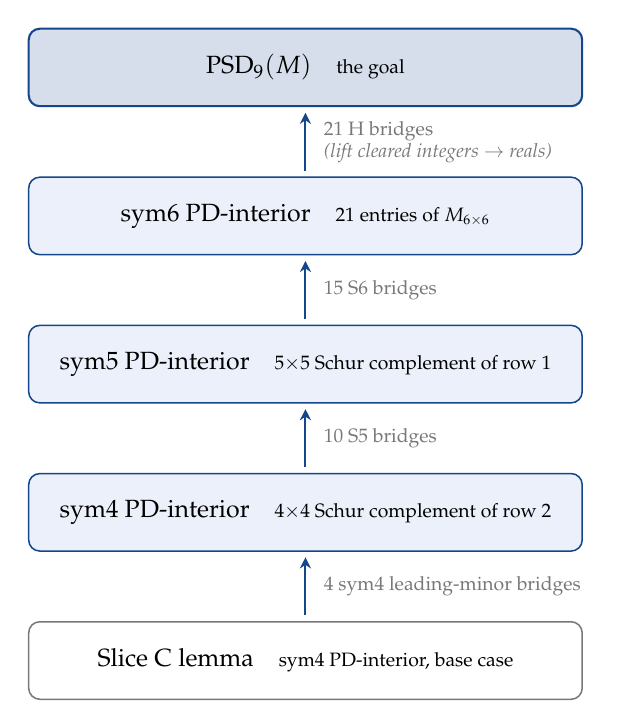
\begin{tikzpicture}[thiele]
\tikzset{
  cstep/.style={
    draw=thiele@accent, line width=0.55pt,
    rounded corners=4pt,
    fill=thiele@pale,
    inner sep=8pt,
    align=center,
    font=\small,
    minimum width=20em,
    minimum height=2.8em
  },
  goalstep/.style={
    cstep,
    fill=thiele@accent!18,
    line width=0.75pt
  },
  basestep/.style={
    cstep,
    fill=white,
    draw=thiele@gray
  },
  cascadearrow/.style={
    ->, line width=0.7pt, draw=thiele@accent,
    shorten >=2pt, shorten <=2pt
  }
}

\node[goalstep]                       (top) {PSD$_9(M)$\quad\textnormal{\scriptsize the goal}};
\node[cstep, below=2.5em of top]      (s6)  {sym6 PD-interior\quad\textnormal{\scriptsize 21 entries of $M_{6\times6}$}};
\node[cstep, below=2.5em of s6]       (s5)  {sym5 PD-interior\quad\textnormal{\scriptsize $5{\times}5$ Schur complement of row 1}};
\node[cstep, below=2.5em of s5]       (s4)  {sym4 PD-interior\quad\textnormal{\scriptsize $4{\times}4$ Schur complement of row 2}};
\node[basestep, below=2.5em of s4]    (base){Slice C lemma\quad\textnormal{\scriptsize sym4 PD-interior, base case}};

% Arrows go UPWARD (each lower step implies the one above)
\draw[cascadearrow] (s6.north) -- node[right=3pt, font=\scriptsize, text=thiele@gray, align=left]
  {21 H bridges\\\textit{(lift cleared integers $\to$ reals)}} (top.south);
\draw[cascadearrow] (s5.north) -- node[right=3pt, font=\scriptsize, text=thiele@gray, align=left]
  {15 S6 bridges} (s6.south);
\draw[cascadearrow] (s4.north) -- node[right=3pt, font=\scriptsize, text=thiele@gray, align=left]
  {10 S5 bridges} (s5.south);
\draw[cascadearrow] (base.north) -- node[right=3pt, font=\scriptsize, text=thiele@gray, align=left]
  {4 sym4 leading-minor bridges} (s4.south);

\end{tikzpicture}
\caption{The Schur cascade lifts the base-case sym4 PD-interior fact from Slice C all the way up to PSD$_9(M)$. Each arrow is one Schur-complement reduction, a polynomial identity in the correlators and moments. The counts beside each arrow are how many such identities the integer check grinds through at that step, one per matrix entry.}
\label{fig:schur-cascade}
\end{figure}
where $M_{6\times6}$ is what the $9\times9$ collapses to once the Q\textsubscript{1+AB} subsumption identities pin its dependent entries: the projection onto the basis $\{v_{B1}, v_{B2}, v_{11}, v_{12}, v_{21}, v_{22}\}$, after which the $9\times9$ lands in the PSD cone whenever the $6\times6$ residual does. From there it is Schur complements all the way down, and it is the same move you already watched at level 1, run on a bigger matrix. The Schur-complement criterion (Section~\ref{sec:vocab}), the one the level-1 bridge used on its $4\times4$ block, turns a positive-definiteness question about the $6\times6$ into one about a $5\times5$ Schur complement; run it again and the $5\times5$ becomes a $4\times4$; and the $4\times4$ closes by Sylvester's criterion, all four leading principal minors positive. That is the whole soundness argument: a base case and three reductions, each one a Schur step you can carry out by hand, stacked from the $4\times4$ back up to PSD9.

Every reduction is a single polynomial identity in the correlators $E_{ij}$ and the moments $\gamma_k$. To keep the opcode's check decidable and integer-only, each identity is multiplied through by the common denominator $\text{KZ} = \bigl(N_{00} N_{01} N_{10} N_{11} \cdot D_{g_1} D_{g_2} D_{g_3} D_{g_4} D_{g_5}\bigr)^2$, where the $N_{ij}$ are the per-setting trial counts and the $D_{g_k}$ the $\gamma$-bucket denominators, and verified on integers, the same clear-the-denominators move as level 1. It is a lot of arithmetic: one identity per matrix entry, twenty-one across the $6\times6$, fifteen for the first Schur step, ten for the second, four leading minors at the base. The kernel grinds every one. But the grinding isn't the argument; the argument is the iterated Schur reduction above, and a reader who wants to break it breaks the reduction, not the fifty identities. A passing integer check is those reductions holding, and those reductions holding is $M$ in the PSD cone. The check leans on nothing past the two background facts level 1 already leaned on: the decidability of the reals and functional extensionality.

\subsubsection{What this delivers and what it does not}

\textbf{Soundness.} For each of the four Q\textsubscript{1+AB} assertion opcodes, the successful-step condition in its theorem implies symmetry and positive semidefiniteness of the specified $9\times9$ moment matrix at the witness-derived correlators and supplied $\gamma$ values. This is an arithmetic certificate about those entries. The theorem does not construct a physical experiment.

\textbf{Scope.} These theorems establish the four integer-check soundness implications and the associated matrix identities. Physical realization, completeness of the checks, and identification of a moment relaxation with a quantum behavior set require their own arguments. The full correlator elliptope is treated separately below.

\textbf{Accounting.} Each assertion instruction has declared cost $S(\mathit{mu\_delta})\geq1$, charged on both success and failure. The integer test establishes its matrix property; the cost schedule records payment for executing the test. These are separate guarantees. The assertion opcodes preserve \texttt{vm\_certified}; their success is observed through the stated trap and error conditions.

\textbf{Falsification.} Exhibit witness counters and $\gamma$ bucket pairs for which one of the four cert-opcodes does not trap but the resulting $9\times9$ NPA moment matrix is \emph{not} PSD, OR show that the Schur-cascade soundness theorem at any slice is incorrect (an SOS identity wrong, a minors-witness step that does not imply PSD9, a bool decider unsound), OR show that the soundness chain depends on a project-local axiom beyond the two standard-library axioms cited above. The Coq \texttt{Print Assumptions} report is the audit surface: every theorem either lists no new axiom or fails the proof gate.

\subsection{The full correlator set: the elliptope completion}
\label{sec:elliptope}

The fixed orthogonal completion excludes some classical correlators, including every deterministic local strategy. The full elliptope allows the within-party cross moments to vary. \code{ElliptopeCompletion.v} defines membership by existence of a PSD completion and proves inclusion of classical correlators, the Tsirelson bound, and exclusion of the PR box. That is the mathematical object this subsection examines.

The characterization is the one Tsirelson's theorem forces. Take the same $5\times5$ moment matrix, marginals still zero, but stop pinning the two cross moments: let $x$ stand for $\langle A_0 A_1\rangle$ and $y$ for $\langle B_0 B_1\rangle$, both free. Call a correlator tuple $(E_{00}, E_{01}, E_{10}, E_{11})$ \emph{elliptope-realizable} when \emph{some} completion $(x, y)$ makes the matrix PSD (\code{elliptope\_realizable}, defined in \code{ElliptopeCompletion.v}). The existential over $(x, y)$ is the entire difference between the slice and the set: the slice asks whether the point is coherent with one fixed completion, the zero one; the set asks whether any completion works.

Five theorems pin the characterization down, all mechanised, all with \texttt{Print Assumptions} reporting only the same stdlib families as the rest of the CHSH algebra (the classical-reals construction and functional extensionality; zero project-local axioms):

\begin{itemize}
\item \code{deterministic\_strategy\_elliptope}: every deterministic local strategy is in the set. The witness is the honest one, $x = a_0 a_1$ and $y = b_0 b_1$, the cross moments the strategy actually has, and the completed matrix becomes an explicit Gram matrix whose quadratic form is a sum of two squares. All sixteen sign patterns are instances of one parametric theorem. \code{classical\_tightness\_witness\_elliptope} names the sharpest instance: the all-ones strategy, the $\mu = 0$ witness of \code{classical\_bound\_achieved} that the slice gate traps, is elliptope-realizable.
\item \code{turing\_point\_elliptope}: $(1, 0, 1, 0)$, this document's running example of a classically reachable point the slice rejects, is in the set, witnessed by $x = 1$, $y = 0$ and the sum-of-squares decomposition $v_0^2 + (v_1 + v_2 + v_3)^2 + v_4^2$ of its completed quadratic form.
\item \code{elliptope\_convex}: the set is closed under binary convex combination; \code{elliptope\_finite\_mixture} extends that to arbitrary finite sub-convex mixtures by a mechanised renormalization induction (the weight deficit absorbed by the origin, \code{elliptope\_zero}); and \code{lhv\_mixture\_elliptope} composes it with the deterministic theorem: every finite mixture of deterministic sign strategies, which is to say every local-hidden-variable correlator, lands inside. Not by hand-waving from the binary case; the $n$-ary theorem is in the kernel. As a small check on the geometry, the classical point $(1,0,1,0)$ has row squared norms $1^2+0^2=1$ and $1^2+0^2=1$ if the rows are ordered as $(E_{00},E_{01})$ and $(E_{10},E_{11})$, while its columns have squared norms $1^2+1^2=2$ and $0^2+0^2=0$. Transposing the matrix supplies the corresponding column/row counterexample; the distinction matters because the fixed-completion proof uses $E^T E$ and therefore column contractivity.
\item \code{elliptope\_tsirelson}: everything in the set satisfies $S^2 \leq 8$, i.e.\ $|S| \leq 2\sqrt{2}$. The proof is worth a sentence, because the fixed-slice row-norm bound does not hold for arbitrary completions. At $y \neq 0$ the row-norm bound fails, and honestly so: the point $(1, 0, 1, 0)$ itself has a row of norm $\sqrt{2}$. What replaces it is Cauchy--Schwarz run inside the PSD form itself (\code{psd\_cauchy\_schwarz}, derived from the same discriminant lemma the reverse bridge uses): the two budgets $\|B_0 + B_1\|^2 = 2 + 2y$ and $\|B_0 - B_1\|^2 = 2 - 2y$ are coupled through the completion, their product is at most $4$, and $S^2 \leq 8$ falls out of that coupling. The bound holds at every point of the set, not because each row is short, but because the completion cannot make both budgets long at once.
\item \code{pr\_box\_not\_elliptope}: the PR box has no completion; its $S$ is $4$ and the Tsirelson theorem refuses it. And \code{beyond\_classical\_elliptope} exhibits a rational point with $S = 12/5 > 2$ inside the set, so the containment of the classical polytope is strict: classical $\subset$ elliptope $\subset$ no-signaling, with both inclusions proper, from inside the formalization.
\end{itemize}

The correlator geometry has three distinct sets: the classical polytope and the zero-marginal slice intersect without containment, and both sit inside the elliptope, which admits every honest classical point the slice refuses while still refusing everything past $2\sqrt{2}$.

The completion gate is executable. \code{ElliptopeGate.v} builds the decidable check an opcode can branch on (\code{elliptope\_check\_full}), in the same integer-only discipline as \code{column\_contractive\_check\_witness}: no real and no rational evaluated at runtime, every denominator cleared into $\mathbb{Z}$. The check has two branches. The PD branch is the cheap path for a strictly-interior point: it takes completion buckets for $(x, y)$, exactly the bucket-pair idiom the 1+AB opcodes use for their $\gamma$ moments, and runs the fraction-free Sylvester test on the denominator-cleared completed matrix, whose soundness is the same \code{sym4\_qf\_nonneg\_from\_pd} LDLT lemma the Slice-C development proves. The LDL branch checks certificates that can include singular boundary completions: it takes a rational $LDL^{\mathsf T}$ certificate, six subdiagonal entries and four pivots over common positive denominators, and verifies the ten entry equations of $M = LDL^{\mathsf T}$ in cross-multiplied $\mathbb{Z}$-arithmetic. Its soundness (\code{elliptope\_ldl\_check\_sound}) is a sum-of-weighted-squares identity: given the equations, the quadratic form \emph{is} $d_1 P_1^2 + d_2 P_2^2 + d_3 P_3^2 + d_4 P_4^2$. The file proves soundness of this certificate format and supplies concrete accepted boundary points. The load-bearing theorem is \code{elliptope\_check\_full\_sound}: a passing check entails elliptope membership of the witness-derived correlators, with the check's own passing as its only hypothesis. And the gate computes, not just proves, each by \texttt{reflexivity}: \code{gate\_accepts\_all\_ones} runs the $\mu = 0$ tightness witness through the LDL branch (its all-ones completion is rank-one singular) and it passes; \code{gate\_accepts\_turing\_point} does the same for $(1,0,1,0)$; \code{gate\_accepts\_beyond\_classical} passes the interior $S = 12/5$ point through the PD branch; \code{gate\_accepts\_pythagorean\_boundary} certifies $(3/5, 4/5, 4/5, -3/5)$, whose arcsine sum is exactly $\pi$ by the 3-4-5 triangle so it sits exactly \emph{on} the Tsirelson curve with $S = 14/5 > 2$ ,  a point invisible to the strict PD branch because its completion is singular, reached by the LDL branch with pivots $(1, 1, 0, 0)$ at $x = y = 0$; and \code{elliptope\_full\_gate\_never\_accepts\_pr\_box} proves no completion buckets and no certificate ever get the PR box through, not by enumeration but by soundness plus the Tsirelson theorem closing both branches at once. This certificate format requires rational completion data. Soundness and the accepted examples do not establish completeness for every elliptope point, or an impossibility theorem about other exact certificate formats.

The runtime \texttt{CHSH\_LASSERT} opcode checks the fixed orthogonal slice. Connecting \code{elliptope\_check\_full} to an opcode requires its instruction semantics, cost rule, and hardware implementation. The completion results concern correlators; they do not characterize the full behavior set with marginals. Identifying the completion model with physical quantum correlators uses external mathematics. Producing entanglement in hardware requires physical evidence. The direct mathematical challenges are concrete: a deterministic sign pattern whose completed Gram matrix has a negative quadratic form would kill \code{deterministic\_strategy\_elliptope}; an elliptope-realizable tuple with $S^2 > 8$ would kill \code{elliptope\_tsirelson}; a PSD completion for the PR box would kill \code{pr\_box\_not\_elliptope} and Tsirelson with it.

%===========================================================================
\section{Irreversibility accounting and the \texorpdfstring{$\mu$}{mu}-hierarchy}
\label{sec:landauer}
%===========================================================================

\subsection{The Landauer association is motivation only}

Same shape as Landauer's 1961 argument: erasing one bit must release at least $kT \ln 2$ of heat into the environment ($k$ Boltzmann, $T$ absolute temperature, $\ln 2$ the natural log of 2). The Coq proofs below do not depend on Landauer being right about the physics. They formalise a conservative accounting indicator at the instruction level: a cost-positive instruction contributes one to \texttt{irreversible\_bits} by definition. That label is bookkeeping, not a proof that the instruction erased information or was physically irreversible. The count of positively charged firings is bounded by total $\mu$. Shape borrowed, content paid for separately.

\begin{theorem}[$\mu$-Landauer step bound]
Let $\texttt{irreversible\_bits}(i)$ be the indicator function that returns $1$ if $\texttt{instruction\_cost}(i) > 0$ and $0$ otherwise. Let $\code{total\_irreversible\_bits}(\textit{trace}) := \sum_{i \in \textit{trace}} \texttt{irreversible\_bits}(i)$. Then for every trace,
\[
\code{total\_irreversible\_bits}(\textit{trace}) \;\leq\; \texttt{trace\_total\_cost}(\textit{trace}).
\]
The Coq witness is \code{total\_irreversible\_bits\_le\_cost}.
\end{theorem}

\begin{proof}
Per-instruction inequality: for every $i$, $\texttt{irreversible\_bits}(i) \leq \texttt{instruction\_cost}(i)$. Two cases.

\emph{Case $\texttt{instruction\_cost}(i) = 0$.} Then $\texttt{irreversible\_bits}(i) = 0$ by definition, and $0 \leq 0$ holds.

\emph{Case $\texttt{instruction\_cost}(i) > 0$.} Then $\texttt{irreversible\_bits}(i) = 1$, and the cost schedule (Section~\ref{sec:mu}) gives $\texttt{instruction\_cost}(i) \geq S(\delta) \geq 1$ for cert-setters or $\texttt{instruction\_cost}(i) \geq \delta \geq 1$ otherwise. So $1 \leq \texttt{instruction\_cost}(i)$.

Summing the per-instruction inequality over the trace:
\begin{multline*}
\sum_{i \in \textit{trace}} \texttt{irreversible\_bits}(i) \;\leq\; \sum_{i \in \textit{trace}} \texttt{instruction\_cost}(i) \\
{} =\; \texttt{trace\_total\_cost}(\textit{trace}).
\end{multline*}
The right equality is by definition of \texttt{trace\_total\_cost} (or via the Latent-$\mu$ theorem applied to the trace from $\mu_0 = 0$). \qed
\end{proof}

\begin{plainreading}
Each cost-positive instruction contributes at least $1$ to total cost and exactly $1$ to the indicator. Sum across the trace and the count is bounded by the cost. A $0/1$ indicator bounded by what it indicates. All it shares with Landauer is the shape: a lower-bound quantity attached to an event. It is not an irreversibility theorem. No physics in the proof. No microscopic erasure model. No physical entropy. No Boltzmann constant. The conversion of $\mu$ counts to joules is the calibration hypothesis (\code{mu\_landauer\_unruh\_calibrated}, Section~\ref{sec:unknown}). No kernel theorem uses it.
\end{plainreading}

The physical claim has to pass a consistency test. \code{calibrated\_model\_exists\_iff\_positive\_cost} characterizes when the abstract positive-dissipation and upper-calibration premises can hold together. The explicit Boolean reset model has an instance. But retaining the previous state in a history list makes every fixed-instruction step injective while preserving its observed transition. \code{zero\_cost\_vm\_jump\_has\_injective\_history\_lift} applies this construction to the zero-cost F1 counterexample. The PC can collapse to one while the larger state retains its past. I cannot identify physical erasure by watching that PC alone.

\medskip
\noindent\textbf{The physical question is still open.} I want to know whether the formal charge has a defensible physical interpretation. Counting positively charged instructions does not answer that question. Neither does the finite-map Python demonstration: it checks its combinatorial model, not heat released by a device. The F1 counterexample makes the next requirement concrete. Build a physical model whose premises can hold together, account for retained history, and then justify the connection to an experiment. Until that is done, the VM ledger gives no measured energy price for certification.

\subsection{The \texorpdfstring{$\mu$}{mu}-hierarchy}

Borrow the silhouette of the classical time-hierarchy theorem, and then say honestly how much smaller the thing inside it is. The shape is the part everyone knows: more of the resource buys you something you provably could not have had with less. The resource here is $\mu$, and the something is a certification level: traces are classified by an executed \texttt{CERTIFY} whose declared charge is at least $k$. Every level $k \geq 1$ is reachable by a one-instruction witness that pays exactly $k$, and no trace in that level can cost less than $k$. That pairing, reachability on one side and a conservation floor on the other, is the whole content. It is not a statement that one problem class outruns another. Whether more $\mu$ ever buys a genuinely harder problem is a different and much heavier question. It is open, I have it on the list in Section~\ref{sec:unknown}, and I am not going to quietly borrow its weight here while it is still unpaid.

\begin{theorem}[$\mu$-Hierarchy (\code{mu\_hierarchy\_theorem})]
Call a trace \emph{level-$k$ certified} when it ends with $\texttt{vm\_certified} = \texttt{true}$ and its executed-instruction log contains a \texttt{CERTIFY} whose charge $S(\delta)$ is at least $k$. For every $k \geq 1$:
\begin{enumerate}
\item There exists a level-$k$ certified trace with total cost exactly $k$.
\item Any level-$k$ certified trace has $\texttt{trace\_total\_cost} \geq k$.
\end{enumerate}
\end{theorem}

\begin{proof}
\emph{Part (1): the level-$k$ witness.} The one-instruction trace $[\texttt{instr\_certify}\,(k-1)]$ does it: the single \texttt{CERTIFY} charges $S(k-1) = k$, which certifies at level $k$ by definition, sets $\texttt{vm\_certified}$ to \texttt{true}, and is the whole bill. Total cost exactly $k$.

\emph{Part (2): cost lower bound.} The level-$k$ hypothesis hands over an executed \texttt{CERTIFY} with $S(\delta) \geq k$; the kernel proof finds it by scanning the executed-instruction log. That one step charged at least $k$ to the ledger, every other step charged at least $0$, and by Latent $\mu$ the total cost is the sum of the step charges, so the total is at least $k$. The scan earns the floor from the certifying step itself.

Each level $k \geq 1$ is therefore realizable at cost exactly $k$, and no trace certifies at level $k$ for less. \qed
\end{proof}

\begin{plainreading}
Two parts. Part (1) is by construction: use the one-instruction trace \texttt{CERTIFY}$(k-1)$. Its charge is $S(k-1)=k$, it ends certified, and there is no padding instruction. Part (2) is the trace-side lower bound: the executed level-$k$ \texttt{CERTIFY} appears in the ledger with cost at least $k$, so the total cost is at least $k$. For the smallest nontrivial example, $k=2$ is exactly \texttt{CERTIFY}$(1)$, which costs $S(1)=2$.
\end{plainreading}

\begin{corollary}[\code{mu\_hierarchy\_no\_upper\_bound}]
No fixed $\mu$-budget suffices for all certification levels.
\end{corollary}

\begin{proof}
Suppose for contradiction that some fixed budget $B \geq 0$ suffices for all certification levels, meaning every certified trace satisfies $\texttt{vm\_mu} \leq B$. Apply the $\mu$-Hierarchy theorem at $k = B + 1$: there exists a certified trace with $\texttt{vm\_mu} = B + 1 > B$, contradicting the budget bound. \qed
\end{proof}

\begin{plainreading}
For any budget you propose, the hierarchy theorem produces a certified trace that exceeds it by $1$. So no finite budget caps all certifications.
\end{plainreading}

What this comes down to is that the ledger does not give discounts. Pick any integer level you like and there is a certified trace that arrives at exactly that level; try to reach it for one unit less and you cannot, not because anybody forbade it but because the cost was already spent on the way up and conservation will not let you unspend it. That is the entire argument, and where it is mechanised the check agrees. Notice what I did not say. I did not say more $\mu$ makes the substrate ``strictly more powerful''. That phrase belongs to the problem-class reading, the question of whether a bigger budget cracks problems a smaller one cannot, and this theorem does not touch it. I would rather leave that fence standing in plain sight than collect on a claim I have not paid for.

Here is the classical statement the shape comes from, so you can see exactly where the resemblance starts and where it stops. The time-hierarchy theorem says that for a time-constructible bound $T(n)$ there are problems you can solve in time $T(n) \log T(n)$ that you cannot solve in time $T(n)$: hand the machine a little more clock and it can decide things it could not decide before. That is a statement about which problems are in reach. The $\mu$-hierarchy keeps the silhouette and trades the cargo: more $\mu$ buys more certification levels, which is a statement about how high the ledger can climb, not about which problems come into reach. It does not use the classical theorem, and it does not define a single time-bounded class. So treat the resemblance as a way to see the result, not as a smuggled inheritance of the classical theorem's strength. The proof a few lines up is the part actually holding weight; the analogy is just the light I am reading it by.

A direct counterexample would be a $k \geq 1$ trace reaching $\texttt{vm\_certified} = \texttt{true}$ and $\texttt{vm\_mu} \geq k$ with total trace cost $< k$. Under the theorem's premises that cannot happen; if it does, the cost accounting or the proof is wrong.

%===========================================================================
\section{Discrete Geometry over Partition Graphs}
\label{sec:geometry}
%===========================================================================

The partition graph can be studied as a combinatorial object with an assigned angle model. The result below is conditional on explicit incidence and boundary-count hypotheses; it requires no physical interpretation.

\subsection{Discrete triangulation of the partition graph}

A partition graph is not only a bookkeeping structure. You can also read it as a shape, a discrete geometric object, and put geometric questions to it. The honesty of the framing matters here, so I will be plain about what is and is not being claimed. The result below reads the partition graph as a triangulated combinatorial object, a graph cut into triangular pieces, and sets it in an equilateral angle model: every corner of every triangle contributes $\pi/3$ radians, which is 60 degrees, because the three angles of an equilateral triangle are equal and a full turn is $2\pi$ radians, or 360 degrees. Those angles are a modeling choice. They are not pulled out of $\mu$ costs, and I am not going to dress them up as if they were.

A discrete triangulation defines a curvature-like angle defect. As I understand it (I researched this for the project, so check me on the geometry): on a flat surface, if you draw a triangle, the interior angles sum to $180^{\circ}$. On a curved surface, the angles can sum to more or less than $180^{\circ}$. Curvature is the amount by which triangles deviate from flat. For an interior vertex of a triangulated surface, the usual discrete curvature is $2\pi$ minus the incident angle sum. At a boundary vertex, the corresponding boundary turning contribution uses $\pi$ instead. The quantity used in the Coq result below uses $2\pi$ at every vertex; on a surface with boundary it therefore includes an extra boundary contribution.

I went looking for the right invariant and found the Euler characteristic $\chi$, a number that captures the overall shape of a triangulated surface, independent of how you draw the triangles. For any triangulation with $V$ vertices, $E$ edges, and $F$ triangular faces: $\chi = V - E + F$. As I read it, no matter how you triangulate the same surface, you get the same number. For a sphere, $\chi = 2$. For a torus (donut shape), $\chi = 0$. The continuum Gauss-Bonnet theorem (which I am citing, not certifying) says the total curvature of a closed surface equals $2\pi\chi$: the local geometric information (curvature) integrates to a global topological fact (shape). The discrete analogue is stated below. The continuum result is exposition.

\subsection{The restricted angle-defect identity}

The definition \code{well\_formed\_triangulated} bundles properties of a partition graph, including triangle and incidence conditions and the additional equation $B=3\chi$. That equation is a hypothesis, not a general theorem about triangulated disks. For example, a disk made by dividing a quadrilateral into two triangles has $V=4$, $E=5$, $F=2$, $B=4$, and $\chi=1$, so it fails this extra condition. The predicate does not separately construct a planar embedding or establish every topological property of a disk.

\begin{theorem}[Restricted angle-defect identity (\code{discrete\_gauss\_bonnet})]
Let $g$ be a partition graph satisfying \code{well\_formed\_triangulated}. In addition to its graph and triangle conditions, this predicate requires $3F=2I+B$, the triangle-incidence degree sum $\sum_v\deg(v)=3F$, and $B=3\chi$, with $\chi=V-E+F$. The edge definitions give $E=I+B$. Assign angle $\pi/3$ to every triangle corner and define
\[
D(g)=\sum_v\bigl(2\pi-\deg(v)\pi/3\bigr),
\]
including the same $2\pi$ term at boundary vertices. Then $D(g)=5\pi\chi(g)$.
\end{theorem}

\begin{proof}
The required triangle-incidence sum gives $D=2\pi V-\pi F$. From $E=I+B$ and $3F=2I+B$, we get $B=2E-3F$. Consequently,
\[
D-2\pi\chi
= (2\pi V-\pi F)-2\pi(V-E+F)
=\pi(2E-3F)=\pi B.
\]
The additional hypothesis $B=3\chi$ now gives $D=2\pi\chi+\pi B=5\pi\chi$.
\end{proof}

\begin{plainreading}
The coefficient follows from both the definition of $D$ and the boundary-count restriction. Coq checks their consequence; it does not establish that the restriction is forced by computation, topology in general, or nature. Removing $B=3\chi$ from the assumptions leaves the more general algebraic expression $D=2\pi\chi+\pi B$ under the incidence equations, rather than a universal $5\pi\chi$ law.
\end{plainreading}

For a triangulated surface whose boundary is a union of simple cycles, the number of boundary vertices equals $B$. Replacing $2\pi$ by $\pi$ at those boundary vertices subtracts $\pi B$, giving the usual combined interior-curvature and boundary-turning total $2\pi\chi$. This explains the relation to discrete Gauss--Bonnet. It requires identifying the boundary vertices and the appropriate surface hypotheses. The existing Coq theorem proves the defined $D$ identity under its own predicate; it does not formalize that boundary-corrected theorem.

For a simple equilateral triangle, the distinction is visible without any machinery. Summing $2\pi-\pi/3$ at its three vertices gives $5\pi$. Summing the boundary terms $\pi-\pi/3$ gives $2\pi$. The first sum is the quantity defined here; the second is the boundary turning total. Both calculations can be right while answering different questions.

I did not write these proofs by hand. I directed LLMs and used the checker to test the formal statements. That method still leaves me responsible for checking the definitions and the interpretation. The $5\pi$ identity is a conditional combinatorial result, not evidence for a new physical constant or a derivation of angles from $\mu$ cost.

%===========================================================================
\section{The substrate and its halting-shaped wall}
\label{sec:substrate-undecidability}
%===========================================================================

The Thiele Machine is not the 51 opcodes. The 51 opcodes are scaffolding. They make the substrate concrete enough to verify in Coq, run as OCaml, and synthesize to silicon, but they are not the substrate itself. The substrate is the step relation together with the cost-ledger monotonicity rule: every atomic transition either preserves $\mu$ or charges it. PNEW, MORPH, CHSH\_LASSERT, the whole instruction set. Those are the experimental apparatus that gives the substrate a concrete realization to probe. Strip the opcodes and the substrate is still there. Add different opcodes that respect the substrate's monotonicity discipline and the substrate is still the same substrate.

The Turing machine has the same shape. Tape, head, and transition table are scaffolding for one realization. Register machines, lambda calculus, counter machines, RAMs, and partial recursive functions all instantiate the same step-relation primitive with different scaffolding; the equivalences between them are theorems, and that this class captures effective computation at all is the Church-Turing thesis. They are all the Turing machine in the sense that matters. Their primitive steps and cost models can differ even when their computable functions agree.

The result that follows is a fact about the substrate, not about the 51 opcodes. The opcodes are one realization. Other substrates that supply the same typeclass fields inherit the same theorem the moment they are presented.

\medskip
\noindent\textbf{Relationship to Rice's theorem.} The result that follows is Kleene's 1938 diagonal pattern instantiated at the substrate level. Rice's 1953 theorem applies the same diagonal to non-trivial extensional properties of recursive functions computed by Turing machines; the substrate-level version below applies the very same diagonal to non-trivial extensional predicates of substrate programs in any model that exposes an internal recursion theorem and an internal representability predicate. It is the same trick, two floors apart, which is the whole point. The formal content is the diagonal construction; what the substrate-level framing adds is the parameterization (any substrate satisfying the typeclass interface, not just the standard Turing model) and the choice of extensional predicate (\texttt{AdmitsShortcut}, branching on \texttt{csr\_cert\_addr} reachability). The result is therefore a substrate-level instance of the pattern Rice used; the result does not fall out as a corollary of Rice's theorem in its original setting, because Rice's premises are about partial recursive functions in the Turing-machine model, and nothing in them knows about arbitrary substrates carrying their own recursion theorems and representability predicates. The formalized result should be read with its own interface premises. Its proof structure does not establish a non-reducibility or Turing-degree separation from classical halting.

\subsection{The Substrate typeclass}

A Coq typeclass is a checklist of operations and properties a type has to supply to count as the thing. The \code{Substrate} interface used here packages the following data and premises independently of any particular instruction set. It does not itself contain a certification predicate or A2:

\begin{itemize}
\item A type \texttt{state} of substrate states.
\item A type \texttt{Program} of substrate programs.
\item An outcome function \texttt{run : Program $\to$ state $\to$ option state}. The record does not impose a correspondence between this function and \texttt{step}, or a divergence interpretation of \texttt{None}; those require an instance contract. The VM instance always returns \texttt{Some} of its 1000-fuel result, including when that result has not halted.
\item A cost function \texttt{mu : state $\to$ nat}.
\item An atomic step relation \texttt{step : Program $\to$ state $\to$ state $\to$ Prop}.
\item A cost-ledger monotonicity field \texttt{mu\_monotone}: \texttt{forall p s s', step p s s' $\to$ mu s $\le$ mu s'}. This is a separate general-purpose monotonicity property from the kernel's A2 (which specifically asserts that a step flipping certification false-to-true costs $\geq 1$, and which is carried by the \code{CertificationSystem} record, not by this typeclass). Both properties hold in the VM: all instruction costs are non-negative and the cert transition costs $\geq 1$. See Section~\ref{sec:axioms} for the A2 statement and the related axioms A3 through A6.
\item A Gödel coding: functions \texttt{encode : Program $\to$ state} and \texttt{decode\_safe : state $\to$ Program} with the round-trip property \texttt{decode\_safe (encode p) = p}. This states recovery by the supplied mathematical decoder; it does not assert that a program in the substrate can execute that decoder or inspect the encoded field.
\item An internal-representability predicate \texttt{Representable : (Program $\to$ Program) $\to$ Prop}, scoping which Coq function transformers the substrate can express as programs of its own kind. Concrete substrates instantiate this with a precise meaning; the minimal nat-coded substrate defines \texttt{Representable f} as ``\texttt{f} is the diagonal flip transformer for the substrate's own decide function,'' which is exactly the shape the diagonalization needs.
\item A recursion-theorem field, internal form: for every internally representable transformer \texttt{f : Program $\to$ Program}, there is a program \texttt{p} extensionally equivalent to \texttt{f p}, where extensionally equivalent means the two give the same result on every input, however differently they are written.
\end{itemize}

The recursion-theorem field is the load-bearing piece. It is the substrate's Kleene 1938 recursion theorem, restricted to transformers the substrate can actually express. The restriction is not a hedge; it is the substrate's own scope. Turing 1936 did not prove ``no decider exists in any conceivable mathematical universe''; he proved ``no Turing machine decides halting,'' because Turing machines were the substrate Turing was studying. The restriction to internally representable transformers is the same scope move at the substrate level: the substrate's limitative theorem is about what the substrate itself can express, not about every Coq function that exists in the meta-theory.

The recursion theorem is not derivable from \code{mu\_is\_initial\_monotone} (the cost-functional uniqueness result). Initiality of the cost functional states that a measure initialized to zero and satisfying the exact increment law \texttt{M (vm\_apply s i) = M s + instruction\_cost i} agrees with $\mu$ on reachable states. It does not select the instruction-price schedule, identify measures on unreachable states, or collapse all monotone measures to one inhabitant. The recursion theorem instead supplies extensional fixed points for transformers satisfying the chosen representability predicate. In the nat construction it is proved separately for each parameter $d$, whose flip determines that instance's restricted representability class and code-2 behavior.

\subsection{The shortcut-admittance predicate}

The substrate becomes interesting for the limitative result when it is equipped with a non-trivial \emph{shortcut-admittance predicate}: a Prop-valued predicate \texttt{AdmitsShortcut} on programs, witnessed by at least one program that admits and at least one that does not, and depending only on extensional behavior (programs with the same \texttt{run} behavior on every state admit shortcuts iff each other).

The typeclass extension \code{WithShortcutPredicate} packages this: an \texttt{AdmitsShortcut} field, two canonical witnesses \texttt{yes\_program} and \texttt{no\_program} with their respective inhabitedness or non-inhabitedness lemmas, and the extensionality field. These are the conditions the diagonalization needs. A substrate that supplies them earns the limitative theorem.

The kernel constructs a concrete nat-coded family and a VM instance parameterized by its representability class and recurrence premise.

For each $d:\mathbb N\to\mathrm{bool}$, \texttt{nat\_substrate d} supplies the typeclass fields for a language with distinguished codes 0, 1, and 2. Its representability predicate selects the flip transformer associated with $d$, and code 2 supplies its fixed point. The theorem \code{nat\_self\_undecidable} states that $d$ fails to decide \texttt{nat\_admits d}. The global assumption report is closed; $d$ remains an explicit mathematical parameter.

The 51-opcode VM substrate \texttt{vm\_substrate} is parameterized over the VM-specific Gödel encoding (\texttt{vm\_encode}, \texttt{vm\_decode\_safe}, the round-trip), the VM's internal-representability predicate (\texttt{vm\_representable}), and the VM's internal recursion theorem restricted to representable transformers. The Coq Section discipline is identical to the one the physical bridges use for their named constants: the parameters are not global axioms; closing the surrounding Section discharges them as explicit \texttt{forall} premises on every consumer. The encoding is a Section parameter too, though not a live one: the kernel's closed round-trip lemma (\texttt{program\_to\_nat}, \texttt{nat\_to\_program}, no Hypothesis) discharges it, which is exactly what the \code{\_encoded} corollary below does. The VM's internal-representability predicate and bounded recurrence premise remain explicit parameters of the encoded theorem. The generic theorem is independent of this particular VM instance, but still requires its own interface premises. The separate family \texttt{nat\_substrate d} supplies those premises only for its $d$-dependent semantics and representability class; it does not discharge the VM premise.

The VM-side \texttt{AdmitsShortcut} is the extensional predicate ``this VM program's bounded run from \texttt{init\_state} coincides with the bounded run of \code{simple\_morph\_trace}.'' \texttt{yes\_program} is \code{simple\_morph\_trace} itself; \texttt{no\_program} is the empty trace (which produces \texttt{init\_state}, demonstrably distinct from \code{simple\_morph\_final}, since the latter has fired the supra-cert channel and the former has not). The extensionality field is the standard ``equal \texttt{run} on every state implies the predicates agree.'' The instantiation that assembles these into the \code{WithShortcutPredicate} interface lives in the kernel.

\subsection{The substrate-level limitative theorem}

\begin{theorem}[Structural-axis undecidability, substrate-level]
For every Substrate-instance equipped with a WithShortcutPredicate extension, there is no Coq-definable function \texttt{decide : Program $\to$ bool} whose corresponding diagonal flip transformer is internally representable in the substrate and that for all programs \texttt{p} satisfies: \texttt{decide p = true} iff \texttt{AdmitsShortcut p}.
\end{theorem}

\begin{proof}
Assume for contradiction such a \texttt{decide} exists. Define the diagonal flip transformer
\[
\mathtt{flip}(p) \;=\; \begin{cases} \mathtt{no\_program} & \text{if } \mathtt{decide}\,p = \mathtt{true} \\ \mathtt{yes\_program} & \text{if } \mathtt{decide}\,p = \mathtt{false} \end{cases}
\]
By hypothesis, \texttt{flip} is internally representable in the substrate. Apply the substrate's typeclass field \texttt{recursion\_theorem} to \texttt{flip}: there exists \texttt{p} such that $\mathtt{prog\_equiv}\,p\,(\mathtt{flip}\,p)$, where \texttt{prog\_equiv} is the extensional equivalence ``\texttt{run} agrees on every initial state.''

Case-split on \texttt{decide p}. \emph{Case A} (\texttt{decide p = true}): by the bi-implication, \texttt{AdmitsShortcut p}; by definition of \texttt{flip}, $\mathtt{flip}\,p = \mathtt{no\_program}$; by the fixed-point witness, $\mathtt{prog\_equiv}\,p\,\mathtt{no\_program}$; by extensionality of \texttt{AdmitsShortcut} (typeclass field), \texttt{AdmitsShortcut p} iff \texttt{AdmitsShortcut no\_program}. The latter is false (typeclass field \code{no\_program\_refuses}). Contradiction.

\emph{Case B} (\texttt{decide p = false}): symmetrically, by the bi-implication \texttt{$\neg$ AdmitsShortcut p}; $\mathtt{flip}\,p = \mathtt{yes\_program}$; $\mathtt{prog\_equiv}\,p\,\mathtt{yes\_program}$; extensionality yields \texttt{AdmitsShortcut p} iff \texttt{AdmitsShortcut yes\_program}. The latter is true (typeclass field \code{yes\_program\_admits}). Contradiction.

Both cases close. No such \texttt{decide} exists. \code{Print Assumptions structural\_shortcut\_undecidable} returns \texttt{Closed under the global context}.
\end{proof}

\begin{plainreading}
Kleene 1938's diagonal, transplanted from time to structure. Same shape: assume a decider, build a flipper, find a fixed point, watch the program disagree with itself in both cases. The work is in the typeclass: once the substrate has its own recursion theorem, two canonical inhabitants on opposite sides of the predicate, and extensionality, the diagonal lands itself. The conclusion excludes correct deciders whose flips belong to the supplied representability class. Its application to a concrete execution model requires that model's fixed-point premise; the generic proof does not establish it.
\end{plainreading}

\begin{theorem}[Structural-axis undecidability for the nat-coded substrate]
For every Coq function \texttt{d : nat $\to$ bool}, the substrate \texttt{nat\_substrate d} cannot internally decide its own structural-shortcut membership predicate. In particular, \texttt{d} itself is not a correct decider for the predicate of the substrate it parameterizes; the corollary \code{nat\_self\_undecidable} reads off this self-referential conclusion directly.
\end{theorem}

\begin{proof}
For each fixed $d$, the substrate \texttt{nat\_substrate d} supplies every typeclass field constructively: \texttt{Program := nat}; \texttt{yes\_program := 0}; \texttt{no\_program := 1}; \texttt{nat\_run d} is a finite Coq pattern match using $d(2)$; \texttt{prog\_equiv} is pointwise equality of \texttt{run}; \texttt{Representable f} is the precise predicate ``\texttt{f} is the diagonal flip transformer for the substrate's own decide function''; \texttt{recursion\_theorem} is discharged by exhibiting code \texttt{2} as the fixed point of any such transformer (its \texttt{run} is defined to mirror whatever the transformer outputs); \texttt{AdmitsShortcut} is extensional by construction; \code{yes\_program\_admits} and \code{no\_program\_refuses} hold by definitional unfolding of \texttt{run} at \texttt{0} and \texttt{1}. Apply the substrate-level theorem above. The corollary \code{nat\_self\_undecidable} specializes the conclusion to \texttt{d} itself: \texttt{d} cannot be a correct decider for \texttt{nat\_admits d}, cannot answer \texttt{true} exactly when the predicate holds. \texttt{Print Assumptions} on both \code{nat\_structural\_shortcut\_undecidable} and \code{nat\_self\_undecidable} returns \texttt{Closed under the global context}.
\end{proof}

\begin{plainreading}
For each candidate $d$, the construction supplies an instance and proves that $d$ fails on that instance's predicate $P_d$. The instance itself depends on $d$. This family theorem does not exhibit one fixed effective predicate that defeats every effective decider.
\end{plainreading}

\begin{theorem}[Structural-axis undecidability for the 51-opcode VM, conditional on the VM's own recursion theorem]
Assume the VM's internal recursion theorem restricted to representable transformers: for every transformer \texttt{f} on VM programs with \texttt{vm\_representable f}, there exists a program \texttt{p} such that \texttt{vm\_run p} and \texttt{vm\_run (f p)} agree on every initial state. Under that assumption, there is no Coq function \texttt{decide : list vm\_instruction $\to$ bool} whose diagonal flip transformer satisfies \texttt{vm\_representable} and that for all programs \texttt{p} satisfies: \texttt{decide p = true} iff \code{vm\_admits\_shortcut\_extensional p}.
\end{theorem}

\begin{proof}
Instantiate the substrate-level theorem at \texttt{vm\_substrate}. The Gödel encoding piece (\texttt{vm\_encode}, \texttt{vm\_decode\_safe}, the round-trip) enters as Section parameters and is then discharged by the kernel's closed round-trip lemma (\texttt{program\_to\_nat}, \texttt{nat\_to\_program}, no Hypothesis) in the \code{\_encoded} corollary. The VM's internal-representability predicate \texttt{vm\_representable} and the VM's internal recursion theorem restricted to representable transformers are the Section parameters that stay live; closing the surrounding Coq Section discharges them as explicit \texttt{forall} premises on every consumer, the same Section-parameter discipline the physical bridges use for their named constants, and the theorem above states that recursion-theorem premise directly rather than leaving it implicit in the proof. The VM-side \texttt{AdmitsShortcut} is the extensional predicate ``this VM program's bounded run from \texttt{init\_state} coincides with the bounded run of \code{simple\_morph\_trace}''; \texttt{yes\_program} is \code{simple\_morph\_trace}; \texttt{no\_program} is the empty trace, which produces \texttt{init\_state} and so differs from \code{simple\_morph\_final} (where the supra-cert channel has fired). The substrate-level diagonal applies; \code{vm\_structural\_shortcut\_undecidable} is its specialization, carrying the VM-side parameters as premises. The nat family above is a separate application with different semantics. This VM specialization remains conditional on its stated bounded recurrence premise and representability class.

\texttt{vm\_run} returns \texttt{Some (run\_vm 1000 p s)} even when fuel expires before halting. Equality of its two finite-data results is decidable externally. Under the recurrence premise, the flip of that correct external decider must therefore lie outside the chosen representability class. The unbounded relation \code{VMUnboundedExec.vm\_halts\_at} instead requires an existential fuel witness and a halted result. Its determinism and saturation proofs do not identify it with bounded-result equality. A separate development now supplies a fixed 60-instruction interpreter over the natural-valued sibling \texttt{vm\_apply\_u}, with executable variable-width encodings of two-counter programs. The guest branches on a successful nonzero decrement and falls through on zero. This convention matters: the earlier zero-branch guest is a weaker machine and is not used as a universality witness. The new \code{VMUnboundedCM2Bridge.mm2\_halting\_host\_iff} proves equivalence between halting in the pinned Coq Undecidability Library's MM2 semantics and raw execution of this fixed host interpreter on the encoded input. Its correctness, malformed-code exclusion, and divergence contracts are proved independently of any supplied interpreter-correctness premise.

The transferred \code{actual\_unbounded\_host\_synthetic\_undecidability} theorem retains the library's precise synthetic meaning: a Boolean halting decider would enumerate the complement of single-tape binary Turing-machine halting. It is not a proof of the unrestricted proposition \texttt{\textasciitilde{} decidable}, nor a recursion theorem for the full VM ISA. The original word64 machine, bounded equality theorem, and conditional structural-shortcut theorem above are unchanged. No effective-specialization theorem or concrete representability/recurrence instance for the full VM is established by this reduction.
\end{proof}

\begin{plainreading}
The VM theorem is conditional on the bounded recurrence and representability premises printed above. The nat family supplies a separate concrete example for each candidate decider. It does not discharge the VM premise. Unbounded execution and a self-interpreter require their own semantics and proofs.
\end{plainreading}

\subsection{The exact interpreter targets}

The word ``interpreter'' names two different constructions in the current
kernel, and I am keeping both names because they answer different questions.
The 60-instruction construction is the fixed host
\code{cm2\_interpreter\_program}; the selected B3 self-interpreter target is
the separate 122-instruction host \code{self\_interpreter\_program}. Neither
is a full-51-opcode self-interpreter for the physical word64 VM.

\paragraph{The 60-instruction CM2 host.}
The guest syntax is \texttt{CM2InstrU}, with five instructions:
\texttt{HALT}, increment-counter-0, increment-counter-1, and decrement-and-
jump for either counter. A guest configuration is
\texttt{CM2ConfigU = (pc,c0,c1)} with all three components in $\mathbb N$.
The decrement convention is explicit: a nonzero counter is decremented and
the guest jumps to the encoded target; a zero counter remains zero and the
guest falls through to the next address. A finite guest program is packed into
one natural using an executable width selected from the program itself. The
host receives \code{cm2\_total\_config\_encoding ambient p start}; the guest
program, width, guest configuration, and host scratch are encoded in the
initial host state. The host's own state and cost fields are ambient; the
guest counters, PC, and result are carried in the designated host registers.

The bridge the kernel actually proves is
\code{mm2\_halting\_host\_iff}: MM2 halting is equivalent to the existence of
a fuel for which the fixed host reaches \code{cm2\_halted} on the encoded
input. The more local correctness contract is split into both directions:
\code{cm2\_uniform\_interpreter\_simulation\_total} gives a positive finite
host run for every successful guest step, while
\code{cm2\_uniform\_interpreter\_raw\_correct\_total} says that a raw host
run ending in the terminal state has exactly the corresponding guest halt or
fall-off result, and conversely every guest halt has such a host run. Canonical
encodings cannot produce the malformed status
(\code{cm2\_uniform\_interpreter\_raw\_never\_malformed}); malformed packed
data is still part of the host contract and is not silently identified with a
guest halt. Guest divergence is the absence of a finite guest halt witness and
is equivalent to the host never reaching its terminal PC by
\code{cm2\_uniform\_interpreter\_divergence\_total}. The output observation is
\code{cm2\_result} together with \code{cm2\_halted}; host scratch and host
$\mu$ are not guest state.

This CM2 host is a separate reduction/bridge result. It does not establish the
bounded VM diagonal's recurrence premise, and it does not establish a
full-word64 or full-ISA universal interpreter.

\paragraph{The 122-instruction self-interpreter.}
The selected B3 target uses \texttt{GInstr}, the twelve-instruction arithmetic
and control fragment \texttt{HALT}, \texttt{LOAD\_IMM}, \texttt{XFER},
\texttt{ADD}, \texttt{SUB}, \texttt{MUL}, \texttt{AND}, \texttt{OR},
\texttt{SHL}, \texttt{SHR}, \texttt{JUMP}, and \texttt{JNEZ}. Guest register
fields are restricted to registers $0$ through $3$, cost fields to the
representable byte range, and guest values, immediates, and jump targets are
natural numbers without a word64 bound. The executable encoding maps each
guest instruction to a nonzero packed word, chooses a width
\code{g\_width}, and packs the program into the natural \code{g\_code}.
\code{g\_width\_fits} proves that the chosen width represents every
well-formed instruction in the finite guest program; an out-of-range fetch is
the guest's normal no-instruction termination condition.

The host is the literal list \code{self\_interpreter\_program}, whose length
is 122. At an interpreter boundary, the representation relation
\code{h\_rep}/\code{hbc} places the guest registers in host registers
$R0$--$R3$, the guest ledger in $R11$, the guest PC in $R12$, the packed code
and width in $R14$ and $R13$, and leaves scratch registers and ambient
non-register state explicit. Every host instruction has declared cost zero in
this construction; the guest ledger is data in $R11$, not the host's
\texttt{vm\_mu}. The guest step is related directly to the unbounded sibling
semantics by \code{g\_step\_is\_vm\_apply\_u}.

The two directions of the raw result contract are
\code{self\_interpreter\_complete} and \code{self\_interpreter\_sound},
packaged as the biconditional \code{self\_interpreter\_correct}: a terminal
guest run exists exactly when an actual run of the fixed host reaches its end
PC with the corresponding represented guest state. The divergence theorem
\code{self\_interpreter\_divergence} uses the same host run and does not
mistake fuel exhaustion for proof of divergence. For arbitrary packed data,
the host can report malformed words; \code{self\_interpreter\_malformed}
specifies that status, while the canonical encoding of a well-formed guest is
proved never to reach it. Guest HALT, guest fall-off, malformed input, and
divergence are therefore separate outcomes. The construction proves the
selected B3 fragment and its frame relation; it is not advertised as an
unchanged-word64 or full-51-opcode self-interpreter.

\paragraph{The precise Rice/reduction domain.}
The theorem called \code{self\_rice} lives on the \texttt{GInstr} model, not
on the bounded \texttt{vm\_run} predicate and not on the CSR state predicate.
Its input predicate is
\[
  p \longmapsto \texttt{g\_wf\_program}(p)\;\wedge\;\mathsf{Pr}(p),
\]
where $\mathsf{Pr}$ is a predicate on guest programs. The premises are: a
well-formed witness $w$ with $\mathsf{Pr}(w)$; a well-formed never-terminating
program \code{g\_bottom} with $\neg\mathsf{Pr}(\code{g\_bottom})$; and the
well-formed extensionality condition
\code{g\_equiv} $p$ $q \mathbin{\to}
  (\mathsf{Pr}(p) \mathbin{\leftrightarrow} \mathsf{Pr}(q))$. Under those premises,
\code{self\_rice} reduces the complement of the pinned MM2 halting problem to
the complement of this well-formed guest predicate and concludes the
repository's synthetic \emph{undecidable} relation.

The guest-program decider contract is separately named
\code{g\_decides}: a well-formed guest program $D$ must terminate on every
well-formed encoded input and report $\mathsf{Pr}(p)$ exactly by whether its
final guest register 0 equals 1. \code{g\_decides\_decidable} turns that
total guest-program behavior into a Boolean decider for the same predicate,
and \code{self\_rice\_representable} transfers the consequence to the
library's enumerability formulation. Thus ``undecidable'' here means the
formal reduction/enumerability contract supplied by the library; it does not
mean an unrestricted meta-theoretic negation of every possible Coq decision
procedure. The bounded VM outcome equality, the VM's conditional structural
diagonal, and the unbounded CM2 bridge remain separate theorems with separate
domains.

\subsection{The proof, in prose}

The proof is the standard Kleene-1938 diagonal, transported to the substrate.

Assume for contradiction that \texttt{decide : Program $\to$ bool} satisfies the bi-implication. Define the flipping transformer
\[
\mathtt{flip}(p) \;=\; \begin{cases} \mathtt{no\_program} & \text{if \texttt{decide p = true}} \\ \mathtt{yes\_program} & \text{if \texttt{decide p = false}} \end{cases}
\]
This is a total Coq function from \texttt{Program} to \texttt{Program}. The theorem also requires that this particular \texttt{flip} satisfy $\mathsf{Representable}$; total Coq definability alone does not establish that premise. With that premise, apply the substrate's recursion-theorem field to \texttt{flip}: there exists a program \texttt{p} with \code{prog\_equiv} $p$ $(\texttt{flip}\ p)$.

Case-split on \texttt{decide p}.

\emph{Case A: \texttt{decide p = true}.} By the bi-implication, \texttt{p} admits a shortcut. By definition of \texttt{flip}, \texttt{flip p = no\_program}. By the recursion-theorem witness, \texttt{p} is extensionally equivalent to \texttt{no\_program}. By extensionality of \texttt{AdmitsShortcut}, \texttt{p} admits iff \texttt{no\_program} admits. But \texttt{no\_program} does not admit. Contradiction.

\emph{Case B: \texttt{decide p = false}.} By the contrapositive of the bi-implication, \texttt{p} does not admit. By definition of \texttt{flip}, \texttt{flip p = yes\_program}. By the recursion-theorem witness, \texttt{p} is extensionally equivalent to \texttt{yes\_program}. By extensionality, \texttt{p} admits iff \texttt{yes\_program} admits. But \texttt{yes\_program} admits. Contradiction.

Both cases close. No correct total decision procedure for \texttt{AdmitsShortcut} whose flip satisfies the stated representability premise exists in this instance. \qed

The proof is short, because the work is in the typeclass, not in the diagonal. The body runs about 38 lines, of which roughly 16 are actual tactic steps; the rest is the case-split structure and the inline narration. Once the substrate supplies the restricted recursion theorem, two canonical inhabitants, an extensional predicate, and representability of the candidate decider's flip, the diagonal is mechanical. The substrate-level work was assembling the right typeclass; the limitative result is what falls out.

The diagonal does not use A2, the ledger, or a certification predicate. Its contradiction uses the restricted recursion-theorem field, representability of the candidate flip, and the two witnesses and extensionality of \code{WithShortcutPredicate}. Certification supplies a separate interpretation in the VM; the nat family has no certification content. A2 neither supplies the recurrence premise nor establishes a correspondence between the bounded program predicate and the CSR state predicate. Those connections must be proved separately wherever an application requires them.

\subsection{The two-axis picture this completes}

\begin{center}
\begin{tabular}{ll}
\textbf{Time axis} & \textbf{Structural axis} \\
\hline
steps & $\mu$ \\
HALT (Turing 1936) & AdmitsShortcut (above) \\
no Turing decider for halting & no correct decider with a representable flip under recurrence \\
\end{tabular}
\end{center}

The comparison records the diagonal proof pattern under each model's premises. The nat construction gives a candidate-indexed family, and the VM result concerns bounded outcome equality under a restricted recurrence premise. Neither establishes a second fixed effective undecidable problem or a Turing-degree separation. The CSR observation collision below is a separate state-level non-recoverability result.

\subsection{What this closes}

\paragraph{What the substrate-level theorem closes.} A total witness procedure would yield a decider of the same predicate only under an explicit reduction contract: its input is each program $p$ in the theorem's domain; its success is equivalent to \texttt{AdmitsShortcut p}; and it terminates with either a witness or a definite negative answer on every such input. To apply the diagonal, the Boolean decider obtained by testing that success must also have a flip in the supplied representability class. Under these premises the theorem excludes the procedure. A procedure returning a \code{SoundStructuralShortcut} record is not automatically such a reduction: its witness relation must first be connected to this exact program predicate. Partial synthesis, restricted argument inputs, and externally supplied evidence are not excluded by the total-decider theorem.

\paragraph{What the nat-substrate theorem closes.} It constructs a family of instances indexed by the candidate $d$. For each member, $d$ fails on that member's predicate. The generic theorem applies under its representability and fixed-point premises. A fixed-system effective undecidability result requires another instance argument.

\paragraph{What the VM corollary closes.} The 51-opcode VM corollary \code{vm\_structural\_shortcut\_undecidable} is the substrate-level theorem instantiated at \texttt{vm\_substrate}: no representable decider answers \texttt{true} exactly when a VM program admits the extensional shortcut. It carries the VM-side Section parameters as explicit \texttt{forall} premises, in the named-premise style the physical bridges use. The generic theorem does not depend on these particular VM parameters, but its VM application does. The nat family supplies a different instance for each $d$ and cannot replace the VM's bounded recurrence premise. The exclusion applies to deciders whose diagonal flips lie in the supplied representability class.

\paragraph{How to falsify.} Three routes.
\begin{enumerate}
\item A Coq function \texttt{decide : Program $\to$ bool} whose diagonal flip transformer is internally representable in some Substrate plus WithShortcutPredicate instance and that satisfies the bi-implication would force the substrate-level proof to fail at one of its steps, each of which is named in the case-split above.
\item For the nat-coded substrate specifically: exhibit a Coq function \texttt{d : nat $\to$ bool} that correctly decides \texttt{nat\_admits d}. The corollary \code{nat\_self\_undecidable} forbids this; finding such a \texttt{d} contradicts the corollary.
\item For the VM specialization, supply its bounded recurrence premise for the chosen representability class and a correct decider whose particular diagonal flip belongs to that class. A correct external decider alone is not a counterexample: bounded membership is externally decidable, and its flip is excluded by every class satisfying that recurrence premise.
\end{enumerate}

\subsection{The wall the classical configuration cannot see}
\label{sec:structural-axis-orthogonality}

There is one sentence that kills most new ``a computer can't decide this'' results before they get off the ground, and the first time I thought I had one I said it to myself before anyone else could: \emph{you didn't find a new kind of unanswerable question. Your machine is a Turing machine with some extra memory bolted on, the thing you can't decide is just one more ordinary fact about what a program does, and Rice's theorem already says nobody can decide facts like that. Nothing new, nothing sideways to ordinary computation.} I went looking for where that sentence breaks the result, because if it does, I'd spent months on a footnote to Rice. It doesn't. The reason is plain once you see it: a classical machine never gets the whole state. It gets a stripped-down version, the part it can read and write, and my unanswerable question turns on a piece the stripping throws away. Rice's theorem is about an answer a machine can't compute from what it's handed. This is about an answer that was never in what it's handed.

A classical decider has, as its entire input, the Turing configuration $\texttt{forget}\ s : \texttt{TMSnapshot}$, the same four-field projection from the structural-axis section. If the thing it is asked to decide is not a function of $\texttt{forget}\ s$, then no classical decider can be right about it, and not for want of horsepower: what it is deciding is not in what it is given. That is the whole shape of this wall, and it is why it sits beside Rice's rather than under it. Two independent obstructions, on two independent axes.

\begin{theorem}[Structural-shortcut admittance is not classical, \code{structural\_shortcut\_not\_function\_of\_classical}]
There is no function $\texttt{decode} : \texttt{TMSnapshot} \to \texttt{bool}$ such that, for every Thiele state $s$,
\[
\texttt{decode}(\texttt{forget}\ s) \;=\; \texttt{admits\_structural\_shortcut\_bool}\ s,
\]
where $\texttt{admits\_structural\_shortcut\_bool}\ s$ is the reading ``$s$'s certification channel has fired'' ($\texttt{csr\_cert\_addr} \neq 0$).
\end{theorem}

\begin{proof}
Two states reachable from \texttt{init\_state} by executing a trace: \code{run\_cert\_set} runs the minimal \texttt{MORPH\_ASSERT} closure and fires the channel ($\texttt{csr\_cert\_addr} = 650$); \code{run\_cert\_unset} runs the same two-instruction prefix, then a graph-preserving no-op whose $\mu$-cost is chosen to match, leaving $\texttt{csr\_cert\_addr} = 0$. The matched cost makes the two runs land on the same $(\texttt{pc}, \mu, \texttt{regs}, \texttt{mem})$, so $\texttt{forget}\ \code{run\_cert\_set} = \texttt{forget}\ \code{run\_cert\_unset}$ by computation. A \texttt{decode} satisfying the equation would have to return both \texttt{true} and \texttt{false} on that one input. Contradiction. \qed
\end{proof}

\begin{plainreading}
These are reachable witnesses for the CSR predicate, with the same four-field \texttt{forget} projection. The predicate is decidable from full state and cannot be recovered from that projection. The bounded program-equality predicate used by the diagonal is a different definition; no equivalence between these predicates is asserted.
\end{plainreading}

This is the first rung of a short ladder, and I want to be exact about how far each rung reaches, because the honest version is sharper than the inflated one.

\textbf{Observation-dependent oracles.} \code{structural\_axis\_survives\_any\_classical\_oracle} quantifies over oracle answers that are functions of \texttt{forget} alone. Composing such an oracle with a decoder preserves the collision. An oracle supplied independent evidence or full state has a different information domain.

\textbf{The two non-determination directions.} \code{axes\_mutually\_independent} supplies reachable witnesses: the structural channel is not determined by \texttt{forget}, and the program counter is not determined by that channel. \code{structural\_membership\_decidable} computes the channel predicate from full state. These are information-loss statements about specified observations. Rice and Turing-degree conclusions require an effective program model and are not consequences of this state-level collision.

\textbf{The concrete VM encoding.} \code{vm\_structural\_shortcut\_undecidable\_encoded} uses the proven \texttt{program\_to\_nat}/\texttt{nat\_to\_program} round trip, with the code stored in \texttt{vm\_logic\_acc}. It still quantifies over a representability predicate and a fixed-point premise for the bounded \texttt{vm\_run}. An unbounded self-interpreter would concern another execution semantics and would require a correspondence theorem before it could discharge this premise. The separate B3 interpreter uses executable data encoding for an unbounded arithmetic/control fragment; it does not supply this bounded-semantics bridge. Furthermore, \code{no\_logic\_acc\_encoded\_interpreter} proves an input-access obstruction by an explicit equivalent-state relation: every executable step and run commutes with replacing \texttt{vm\_logic\_acc}. A fixed VM program cannot use that encoded input to reproduce even a simulated program's final certification bit through an output observation independent of the retained input code. This rules out the proposed encoding for that interpreter contract; it does not rule out an executable alternative encoding or an architectural extension.

\begin{plainreading}
The state-level theorem excludes recovery from the specified observation, including observation-dependent oracle extensions. The program-level theorem excludes deciders whose flip transformers belong to a representability class satisfying the stated recurrence premise. The nat example is a family parameterized by the candidate decider. These results retain their separate domains and quantifiers.
\end{plainreading}

%===========================================================================
\section{What Coq is, and why I used it}
\label{sec:coq}
%===========================================================================

Coq is a proof assistant, which is a phrase I had to go look up. Underneath the phrase it is a programming language, but one whose type system is strict enough to do a thing ordinary languages cannot: you write a proof down as a program, and the compiler refuses it unless the program genuinely matches the statement you claimed. You cannot talk it into a maybe.

Here is the idea. In a normal programming language, a type says something about what kind of value a variable holds. In Python, \texttt{x: int} means $x$ is an integer. In Coq, types are propositions. The type \texttt{n > 0} means ``the proof that $n$ is positive.'' A function from \texttt{n > 0} to \texttt{n + 1 > 0} is a proof that if $n$ is positive, $n+1$ is too.

The compiler checks whether the types line up. If your proof has a hole and you write ``trust me,'' it rejects you. You can't bluff a proof term past it. But here is the part people skip, and it's the part that matters: the compiler checks that the proof matches the statement. It does not check that the statement says what you meant. Hand it a statement that means nothing and it'll prove it for you, three characters, no complaint. So the compiler accepting a proof is not the same as the thing being true. It means this proof matches this statement, and whether that's the right statement is on me, not the machine.

So I didn't use Coq to make anything true. I used it because I don't trust my own eye to catch a gap in an argument I want to believe. I spent months convinced by my own reasoning, pushed the proof through, and watched a key step come apart in my hands. The machine caught where I'd fooled myself. That is what it's for, and it's the same source the running machine and the chip get extracted from. Gap-catcher and extractor. Not the proof. The proof is the argument, and an argument has to close in a way a person can follow, or it hasn't closed at all.

\subsection{Reproducing the source and proof contracts}
\label{sec:reproduction}

Repository: \url{https://github.com/sethirus/The-Thiele-Machine}. The
repository carries the formal sources, pinned dependency trees, executable
contract probes, and the native reproduction runner. The authoritative
reproduction procedure is documented in \texttt{docs/REPRODUCTION.md}; it
builds a fresh source snapshot and does not rely on patches or precompiled
proof objects.

Use the native toolchain required by the repository, then run the following
commands from the repository root:
\begin{verbatim}
python3 scripts/reproduce_coq.py --jobs 1
python3 scripts/check_coq_probe.py
bash monograph/build_monograph.sh
\end{verbatim}

The source-only reproduction must exit zero. Inspect theorem types and global
dependencies as well as the exit status; a closed report does not discharge
explicit premises. The monograph build regenerates the publication outputs
from the TeX sources. The generated reproduction records are execution
evidence for that run, not additional source files.

RTL generation is a separate command, \texttt{bash scripts/kami\_extract.sh}, requiring the Bluespec compiler and its standard library in addition to the Coq/OCaml toolchain. Its logs, generated Verilog, synthesis report, and any bitstream must carry the source identity they actually used. A successful Coq build supplies no fresh synthesis or timing measurement. The proof-audit output likewise retains the source state and generation date it describes.

\subsection{The Inquisitor}

Beyond Coq's type checker, the project has a custom proof auditor called the Inquisitor, shipped with the proof corpus. It runs on every commit and emits 86 distinct rule codes. The main categories:
\begin{itemize}
\item \textbf{No holes.} No \texttt{Admitted}, \texttt{admit}, or \texttt{give\_up} anywhere in the active proof files. No unproved \texttt{Axiom} or \texttt{Parameter} declarations in project code.
\item \textbf{Vacuity heuristics.} No theorem whose conclusion is literally \texttt{True}, \texttt{0 = 0}, or any other tautology that proves nothing. No ``theorem'' of the form $P \to P$. Existence claims backed by a constant witness get flagged. A flag is a reason to look, not a verdict: some constructions, like a fixed interpreter program, are supposed to be fixed, and they get judged on their premises and on what they actually compute. Coq's kernel already prevents circularly dependent proofs (it checks definitional well-foundedness); the Inquisitor catches separately the case where a proof is technically valid but epistemically empty, proving \texttt{True} by \texttt{trivial}, for instance.
\item \textbf{Physics-definition heuristics.} No physics quantity defined as a constant placeholder. No physics claim without a corresponding invariance condition. No theorem stated about a physics concept if that concept is not genuinely formalized.
\item \textbf{No trivial true proofs.} If a theorem's entire proof is \texttt{trivial} or \texttt{tauto} and the conclusion reduces to \texttt{True}, the theorem is rejected.
\item \textbf{Scope enforcement.} The proof tree is split into tiers. Tier 1 is the kernel files: the core proof of the machine. Tier 1 files may not import from exploratory or research-side files. Theorem connectivity: every file in the active proof tree must reach the cost or semantics foundation through its import chain. If a file is disconnected, it does not get to claim the kernel's pedigree.
\item \textbf{Comment hygiene.} The maintained source and documentation comments
contain no unfinished or historical review markers; the repository checks this
with \texttt{scripts/comment\_hygiene.py} alongside the Coq proof audit.
\end{itemize}

The proof-audit output records the source state from which it was generated.
Regenerate it whenever the source tree changes. The rule checks and their
scope notes are heuristic evidence; they do not prove semantic applicability
or absence of every vacuous premise.

%===========================================================================
\section{Zero Admitted: what it actually means}
\label{sec:zeroadmit}
%===========================================================================

``Zero Admitted'' is literal. Nowhere in the proof tree did I write ``trust me'' and walk on. Every step the checker could see, it saw, end to end, with no ``and the rest is obvious.'' That is a hygiene fact about the gap-catcher, not a verdict on the argument: it says I didn't let myself skip a step where the machine was watching. It does not say the statements are the right statements. That part stays on me, which is what the rest of this section is about.

This is what it does NOT mean:
\begin{itemize}
\item It does not mean the theorems prove physical reality. The theorems prove things about the Thiele substrate, as formalised in Coq. Whether that formalisation describes the world you live in is a separate question, answered by experiments, not by proof checkers.
\item It does not mean the Coq axioms themselves are consistent. Coq sits on a formal foundation called the Calculus of Inductive Constructions. The key idea is the Curry-Howard correspondence: proofs and programs are the same thing. A proof that $P$ is true is literally a program of type $P$. Checking the proof is type-checking the program. The ``inductive'' part means you can define your own recursive types (naturals, lists, trees) inside the system instead of having them as magical primitives handed down from above. That matters. The foundation is explicit. Nothing is smuggled.

Now the honest limitation. The sources I read on Coq's foundation say it is believed to be logically consistent (meaning you cannot derive a contradiction from it), but this has not been proven within Coq itself. The way I understand it, that is not a weakness specific to Coq. The label I dug up is Gödel's incompleteness theorem from 1931: a consistent, effectively axiomatized theory containing sufficient arithmetic cannot prove its own standard arithmetized consistency statement under the usual derivability conditions. And an inconsistent system proves everything, its own consistency included. So Coq's foundation is trusted, not proved-from-within. ``Trusted'' has substance here. The same foundation has verified the CompCert C compiler and the Four Color Theorem (Gonthier 2005, a landmark fully machine-checked proof of a major mathematical theorem, one first settled on paper-plus-computer in 1976), among other artifacts. That prior use is evidence about the foundation's track record in practice. It is not a proof of logical consistency, and a successful large-scale application would not necessarily surface every possible inconsistency; an inconsistent system only breaks visibly if some proof actually exploits the inconsistency, and nothing here rules that out. I am relaying what I read. I have not personally audited CompCert or Gonthier's proof. ``Zero Admitted'' means every theorem follows from those axioms. It does not mean those axioms are themselves in-system guaranteed. It means they are the same axioms a substantial body of verified software has relied on without breaking, which is track record, not a consistency proof.
\item Hardware correspondence is conditional on its model and representation contract. \texttt{driven\_step\_wf} proves intermediate model equality under \texttt{WFDrivenPrecondition}; executable RTL transfer adds finite-range and retirement obligations and toolchain trust. The four Q\textsubscript{1+AB} instructions remain outside the synthesized inventory.
\item It does not mean the OCaml runner binary is proven inside Coq to be bitwise identical to the Coq semantics. The kernel proves Coq-side observable facts. The parity suite checks the extracted binary empirically. One is a theorem. The other is a test.
\end{itemize}

A kernel-checked theorem proves its complete type, including quantified premises and record obligations. A Section hypothesis can become a theorem argument after generalization. \texttt{Print Assumptions} reports global dependencies; \texttt{Closed under the global context} does not remove those arguments. Assessing an intended instance requires its statement, expanded load-bearing definitions, global assumption report, and witnesses for the premises.

The bridges add mathematical premises and external trust boundaries. Physical interpretations require their named quantum or Landauer--Unruh calibration premises. Executable hardware transfer also depends on extraction, the OCaml pretty-printer, BSC, generated RTL, and the simulation harness; synthesis and place-and-route add further tools when silicon claims are made. The Coq model theorem does not verify that whole chain. External OCaml and RTL parity are test results with their own revision and input domains.

%===========================================================================
\section{How to break this}
\label{sec:falsification}
%===========================================================================

Every main claim in this document comes with the exact shape of the thing that would kill it. I went to the trouble on purpose. A claim you can't break is a claim that wasn't saying anything, and I would rather hand you a loaded gun pointed at my own work than a sentence too vague to aim at. So the ones below are written as instructions, not as boasts: here is the trace to find, here is the object to build, here is the theorem to exhibit. Build one and the proof tree falls, and I mean that as the better outcome of the two, because a break tells me something I didn't know and a year of nobody finding one only tells me people got tired of looking. If you build any of these, that is the message I want in my inbox.

\medskip
\noindent\textbf{Falsify No Free Insight.}\\
Find a VM trace that:
\begin{itemize}
\item starts with \texttt{vm\_certified = false} and \texttt{vm\_mu = 0}
\item ends with \texttt{vm\_certified = true}
\item ends with \texttt{vm\_mu = 0}
\end{itemize}
If you find such a trace, the claim is false: \code{certification\_requires\_positive\_mu} breaks at the step that prices the cert-flip. Add the counterexample as a theorem and the check refuses to compile on top of that.

\medskip
\noindent\textbf{Falsify $\mu$-monotonicity.}\\
Find a state $s$ and instruction $i$ such that $(\texttt{vm\_apply}\ s\ i).\mu < s.\mu$. The Coq proof of \texttt{vm\_apply\_mu} falls.

\medskip
\noindent\textbf{Falsify categorical separation.}\\
Show that the two witness states in \code{categorical\_separation} differ in one of the six computational fields (registers, memory, $\mu$, PC, error, certification), or that their morphism lists are the same. Either kills it. Error behavior is not the target; the thing that separates them is the morphism graph itself.

\medskip
\noindent\textbf{Falsify Turing strictness.}\\
Exhibit a \emph{classical} program, a Thiele instruction trace restricted to the classical opcode fragment (\texttt{is\_classical\_program}, run on the same substrate), whose execution changes the partition graph (\texttt{pg\_next\_id}) or the morphism map. Or prove that the witness step \texttt{PNEW} leaves \texttt{pg\_next\_id} fixed. Either kills the strictness half of \code{D5\_thiele\_strictly\_extends\_classical}. This is the semantic claim, that the classical opcode fragment cannot reach the structural states one structural opcode reaches. It is not the computability claim. A Turing machine can of course simulate a Thiele run by encoding the graph as bytes on its tape; that simulation exists and is not a counterexample.

\medskip
\noindent\textbf{Falsify structural entitlement.}\\
Prove that for every pair of Thiele VM states with the same classical shadow and different morphism structure, no probe preserves the distinction; equivalently, refute the concrete witness pair the theorem exhibits. \code{shadow\_strictly\_lossy} falls. Or produce a strict feasible-set subset with a distinguishing observation that does not yield stronger membership predicates. The feasible-subset theorem falls with it.

\medskip
\noindent\textbf{Falsify universal certification cost.}\\
Build a \code{CertificationSystem} satisfying the one-step rule \texttt{cs\_cert\_costs}, then give a trace from uncertified to certified with total cost 0. \code{universal\_nfi\_any\_substrate} falls. If you instead drop the one-step rule, you have found a free-certification system, not a counterexample.

\medskip
\noindent\textbf{Falsify substrate-level structural-axis undecidability.}\\
Three routes (Section~\ref{sec:substrate-undecidability} expands).
\begin{itemize}
\item Exhibit a Coq function \texttt{decide : Program $\to$ bool} whose diagonal flip transformer is internally representable in some Substrate plus WithShortcutPredicate instance and that satisfies the bi-implication. The substrate-level proof of \code{structural\_shortcut\_undecidable} must fail at some step; identify which.
\item For the nat-coded substrate specifically: exhibit a Coq function \texttt{d : nat $\to$ bool} that correctly decides \texttt{nat\_admits d}. The corollary \code{nat\_self\_undecidable} says no such \texttt{d} exists; build one and you have contradicted it head-on, which is exactly the kind of break I want to hear about.
\item For the VM specialization, supply its bounded recurrence premise for the chosen representability class and a correct decider whose particular diagonal flip belongs to that class. A correct external decider alone is not a counterexample: bounded membership is externally decidable, and its flip is excluded by every class satisfying that recurrence premise.
\end{itemize}

\medskip
\noindent\textbf{Falsify the classical CHSH bound.}\\
Exhibit four fixed bits $a_0, a_1, b_0, b_1$ and a tally consistent with that one strategy (\texttt{WCLocallyConsistent}, every setting pair sampled) whose score beats 2. \code{chsh\_stat\_violation\_not\_local} falls. So does known mathematics. A short run from a randomized local strategy that lands past 2 by luck does not count; the theorem is about one fixed deterministic strategy, and Section~\ref{sec:chsh}'s coin-flip example already shows that luck.

\medskip
\noindent\textbf{Falsify the CHSH-NPA bridge.}\\
The biconditional \code{column\_contractive\_iff\_quantum\_realizable} falls to a counterexample in either direction: a column-contractive correlator whose specified zero-marginal, zero-within-party-moment matrix is not PSD (forward), or a PSD specified zero-marginal, zero-within-party-moment matrix whose correlators are not column-contractive (reverse). For the Tsirelson corollary, exhibit a slice-coherent (column-contractive) correlator with $|S| > 2\sqrt{2}$ and \code{state\_column\_contractive\_implies\_tsirelson} falls. The PR box and the Turing-classical point $(1,0,1,0)$ are \emph{not} counterexamples: both fail column contractivity by direct arithmetic, which is what the theorem requires, not what would break it.

\medskip
\noindent\textbf{Falsify the elliptope completion.}\\
Three targets, one per load-bearing theorem of Section~\ref{sec:elliptope}. Exhibit signs $a_0, a_1, b_0, b_1$ with squares 1 and a vector on which the completed Gram form goes negative; \code{deterministic\_strategy\_elliptope} falls. Exhibit an elliptope-realizable correlator tuple with $S^2 > 8$; \code{elliptope\_tsirelson} falls, and with it the claim that the completion cannot stretch both Cauchy--Schwarz budgets at once. Exhibit real $x, y$ making the PR box's completed $5\times5$ matrix PSD; \code{pr\_box\_not\_elliptope} falls. The $\mu = 0$ all-ones witness and $(1,0,1,0)$ are \emph{not} counterexamples here either, in the opposite direction from the bridge entry above: the elliptope theorems admit them, which is what the theorems require.

\medskip
\noindent\textbf{Falsify the elliptope gate.}\\
\code{elliptope\_check\_full\_sound} claims soundness with the check's passing as its only hypothesis: any passing combination of witness counters, completion buckets, or LDL certificate entails elliptope membership of the witness-derived correlators. Exhibit inputs where \code{elliptope\_check\_full} returns \texttt{true} while the correlators lie outside the set (violating $S^2 \leq 8$ suffices), and the soundness theorem falls, taking \code{elliptope\_full\_gate\_never\_accepts\_pr\_box} with it. Trap-side behavior is not a target, and a rejection is never a counterexample to soundness. This gate's certificate format requires rational completion or LDL data (Section~\ref{sec:elliptope}), so by construction it cannot accept a boundary point whose every PSD completion is irrational. That is a fact about this particular certificate format, not a theorem that any exact integer check whatsoever must reject exactly those points and no others; no such general claim is made or needed here.

\medskip
\noindent\textbf{The Inquisitor standard.}\\
Run the Inquisitor on the repository and inspect its output. The command fails on HIGH or MEDIUM findings; LOW findings are reported without independently causing failure. In-source scope markers and their justifications are kept next to the code they describe. This is a syntactic and heuristic audit, not a complete check of theorem applicability or surrounding prose. A new finding requires review rather than an automatic conclusion that a theorem is false.

\medskip
\noindent\textbf{Falsify the axiom audit.}\\
If running \texttt{Print Assumptions} (Section~\ref{sec:vocab}: the Coq command that reports global proof dependencies) on any named theorem in the kernel tier shows a project-local \texttt{Axiom} or \texttt{Parameter} in the dependency tree, the audit has degraded. The current full-corpus probe covers 12,335 named theorems: 5,520 close under the global Coq context outright, and 6,815 use only Coq standard-library assumptions. The receipt names five such constants: dependent functional extensionality, \texttt{Eqdep.Eq\_rect\_eq.eq\_rect\_eq}, \texttt{ClassicalDedekindReals.sig\_not\_dec}, \texttt{ClassicalDedekindReals.sig\_forall\_dec}, and \texttt{Classical\_Prop.classic}. Zero project-local axioms appear in any of the 12,335 dependency trees. This is an audit of global dependency provenance, not a proof that explicit Section-generalized premises hold for a chosen instance; those premises remain visible in theorem types and are audited separately. Any project-local axiom or parameter appearing in a global dependency tree is a bug.

\medskip
\noindent\textbf{Falsify the hardware bisimulation.}\\
A counterexample to \texttt{driven\_step\_wf} must satisfy \texttt{WFDrivenPrecondition} and falsify its stated intermediate model equality. A cosimulation mismatch on a valid represented input challenges the tested RTL transfer for that revision. Diagnose encoding, observation timing, extraction, pretty-printing, BSC, and harness behavior separately. A rejected input outside the theorem's domain or a toolchain mismatch does not refute the conditional Coq theorem.

\medskip
\noindent\textbf{Falsify the convergence answer to parametricity.}\\
The separation/minimality/uniqueness trio is schema-parametric: any field a step rule carries that classical state does not determine supports all three theorems, word for word, and I concede that in full. What singles out certification is convergence: the verifier factorisation result (\code{V\_does\_not\_factor\_through\_classical}), the clean-room floor demonstration (\code{nofi\_demo}), and the NPA moment-matrix certificate (\code{chsh\_lassert\_no\_trap\_implies\_quantum\_realizable}) land on the same field from vocabularies that owe each other nothing. Exhibit another field with three convergent bridges of the same standing, or break one of these, and certification's distinguished seat falls back to an aesthetic choice. Whether certification is the event a model is \emph{forced} to price remains the named open problem either way; Section~\ref{sec:pointer} states the conjectured criterion (redundant record proliferation) that a successor project would have to prove or refute, with its own attack surface listed there.

\medskip
\noindent\textbf{Falsify the proof-of-stake reduction.}\\
Construct a trace in the formal finality model satisfying the stated slashing schedule, with unfinalized initial state, finalized final state, and zero summed modeled charge. This contradicts \code{slashing\_finality\_floor}. A deployment with different transition or accounting semantics instead challenges its proposed interpretation.

\medskip
\noindent\textbf{Falsify the gas-metering reduction.}\\
Construct a schedule satisfying both the commitment floor and no-overcharge whose charging predicate differs from the commitment predicate on some reachable step. \code{gas\_schedule\_exactness} falls, and the kernel's \code{exact\_commitment\_pricing\_characterization} with it.

\medskip
\noindent\textbf{Falsify the attestation reduction.}\\
Build a sound and complete attestation verifier for the $\mu$-dependent claim that reads only the bare classical transcript, a function of the report's log field alone. \code{attestation\_cannot\_factor\_through\_bare\_transcript} falls, and behind it the verifier-factorisation theorem.

\medskip
\noindent\textbf{Falsify the transparency-log reduction.}\\
Build a sound and complete log-free verifier with the same soundness target. \code{log\_free\_verifier\_impossible} falls, and the bare-setting impossibility with it.

\medskip
\noindent\textbf{Falsify the proof-carrying reduction.}\\
Construct a level-$k$ certified proof script with total $\mu$ below $k$, or a sound and complete zero-round bare verifier. \code{level\_k\_verification\_floor} or \code{bare\_pcc\_impossible} falls, and the $\mu$-hierarchy or the bare-setting impossibility behind them.

%===========================================================================
\subsection{Contribution and attribution boundary}
\label{sec:attribution}

This section says what is mine and what is not. It is not a claim to have been first. I have not read widely enough to say any result below is historically new, and I am not going to pretend otherwise. Two comparisons earlier in the document are primary: Landauer's erasure result and Wolpert and Macready's No-Free-Lunch theorem. The other labels are orientation points, and I would welcome correction on any of them.

The work comes apart into five layers.

\begin{description}[style=nextline,leftmargin=0pt,itemindent=0pt,labelsep=0.5em,font=\bfseries]
\item[Borrowed mathematics and vocabulary.] Category theory, Turing and Church--Turing terminology, the Kleene and Rice diagonal patterns, Bell, CHSH and Tsirelson, NPA and the elliptope, the thermodynamic motivation, and the ordinary definitions of projections, partitions, predicates and resource measures all come from other people and from standard mathematics. None of it is mine.

\item[Formal reconstructions.] The Coq development defines the state types, transition systems, fixed real-matrix predicates, encodings and proof terms this monograph uses. When I say a theorem is checked in Coq, I mean the stated proposition has a kernel-checked proof under its printed premises. That does not make the underlying idea mine, and it does not make it new.

\item[Results I developed and proved here.] Inside the stated interfaces, the repository proves the abstract A2 certification floor, the fixed-schedule ledger identity and uniqueness, the named projection-separation witnesses, the trace-fold universal property, the conditional structural-entitlement representation theorem, and the substrate-diagonal results. These are claims about the explicit Coq contracts and witnesses. They are results of this project. I am not claiming nobody wrote down an equivalent statement before me.

\item[Instances and engineering.] The 51-opcode VM, its cost schedule, the Python and extracted-OCaml runners, the Kami model, the Bluespec and Verilog path, the verification scripts, the finite tests, and the synthesis and FPGA workflow are things I built. How much of each is proved, tested, or trusted is the edge-by-edge account in Section~\ref{sec:hardware} and \texttt{docs/ASSURANCE.md}. A tested edge stays a tested edge. I do not promote it to a theorem.

\item[Open proposals and things I am not claiming.] Whether there is a unique structural core, what the ledger means physically, which priced events are universally necessary, full-ISA hardware equality without conditions, and broad quantum or complexity-theory conclusions are all open or out of scope. Proving a conditional contract does not close any of them.
\end{description}

So the claim ledger that follows is a map from formal names to their domains and premises. It is not a list of discoveries.

%===========================================================================
\section{The full claim ledger}
\label{sec:claims}
%===========================================================================

The following claims are checked in Coq under their complete formal premises. The crosswalk below records the principal domains and instance boundaries; the named source declarations give the full quantified statements.

{\small\raggedright\tolerance=10000\emergencystretch=15pt
\begin{enumerate}
\item \textit{\small no\_free\_certification}: csr\_cert\_addr going $0 \to$ nonzero in one step requires cost $\geq 1$.
\item \textit{\small no\_free\_certification\_mu}: same, with $\mu$ increment $\geq 1$.
\item \textit{\small no\_free\_certification\_trace\_mu}: trace-level version.
\item \textit{\small no\_free\_certification\_certified}: vm\_certified going false$\to$true requires cost $\geq 1$.
\item \textit{\small certification\_requires\_positive\_mu}: both channels covered.
\item \textit{\small universal\_nfi\_any\_substrate}: any abstract certification system satisfying the one-step cost rule has trace-level non-free certification.
\item \textit{\small thiele\_universal\_nfi\_cert\_addr}: universal theorem instantiated for Thiele's \texttt{csr\_cert\_addr} channel.
\item \textit{\small thiele\_universal\_nfi\_certified}: universal theorem instantiated for Thiele's \texttt{vm\_certified} channel.
\item \textit{\small thiele\_represents\_simulating\_cert\_system}: any certification system with a simulation morphism into Thiele transfers certification into a Thiele certified execution.
\item \textit{\small forget\_kernel\_is\_eq\_on\_classical}: the classical snapshot quotient forgets exactly the non-classical fields.
\item \textit{\small blindness\_non\_injective}: distinct Thiele states can have the same classical snapshot.
\item \textit{\small certification\_is\_lost}: certification can be in the kernel of the classical forgetful map.
\item \textit{\small shadow\_strictly\_lossy}: the classical shadow forgets morphism structure.
\item \textit{\small mu\_ledger\_necessity}: no strict-classical oracle on $(\texttt{mem}, \texttt{regs}, \texttt{pc})$ recovers the pair $(\mu, \texttt{certified})$.
\item \textit{\small vm\_mu\_not\_classically\_determined / vm\_certified\_not\_classically\_determined}: neither ledger balance nor certification status is a function of strict classical state.
\item \textit{\small mu\_ledger\_mutual\_independence}: $\mu$ and \texttt{vm\_certified} are each independent of strict classical state and of each other under cost-only/cert-only projections.
\item \textit{\small mu\_ledger\_minimality / P\_full\_complete\_neither\_mu\_nor\_cert\_droppable}: the full $(\texttt{mem}, \texttt{regs}, \texttt{pc}, \mu, \texttt{certified})$ projection is complete, and dropping either $\mu$ or certification destroys the corresponding completeness.
\item \textit{\small thiele\_nfi\_pc\_indexed}: PC-indexed execution version.
\item \textit{\small mu\_is\_initial\_monotone}: $\mu$ is unique given the initial value and fixed instruction-cost schedule.
\item \textit{\small vm\_apply\_mu}: exact ledger identity $(\texttt{vm\_apply}~s~i).\mu = s.\mu + \texttt{instruction\_cost}(i)$. The cost is not just $\delta$, it is $\delta$ for ordinary instructions, $S(\delta)$ for cert-setters, $|\text{payload}|_{\text{bits}} + S(\delta)$ for EMIT, etc.
\item \textit{\small kernel\_certified\_implies\_positive\_mu}: from zero, reaching certified implies $\mu > 0$.
\item \textit{\small feasible\_strict\_subset\_implies\_strict\_predicates}: feasible-set narrowing plus a distinguishing observation yields a strictly stronger predicate.
\item \textit{\small strengthening\_requires\_structure\_addition}: certified predicate strengthening requires a structure-addition event.
\item \textit{\small b4\_information\_reduction\_derives\_strict\_predicates}: feasible-set reduction can generate the strict-predicate premise used by NoFI.
\item \textit{\small info\_priced\_cert\_executions\_bound}: executed cert-setting events are bounded by $\Delta\mu$.
\item \textit{\small observation\_partition\_reduction\_implies\_posterior\_representative\_reduction}: observation classes package into the posterior-representative witness for structural entitlement.
\item \textit{\small info\_priced\_arbitrary\_feasible\_reduction\_bound}: with a decision-tree/representative witness, feasible-set compression is bounded by $\Delta\mu$.
\item \textit{\small info\_priced\_weighted\_feasible\_reduction\_bound}: the $\Delta\mu$ lower bound extends to nat-weighted feasible sets.
\item \textit{\small structural\_entitlement\_representation}: strict narrowing plus distinguishability, certified posterior admissibility, and an explicit posterior-representative reduction imply a strictly stronger predicate, a structure-addition event, and a $\Delta\mu$ lower bound.
\item \textit{\small every\_sound\_structural\_shortcut\_lands\_here}: every packaged \code{SoundStructuralShortcut} instantiates the structural-entitlement representation theorem.
\item \textit{\small structural\_shortcut\_undecidable}: for every Substrate plus WithShortcutPredicate instance, no Coq function whose diagonal flip transformer is internally representable in the substrate decides the structural-shortcut admittance predicate. The substrate's own halting-shaped wall, by Kleene 1938 diagonal restricted to the substrate's internal expressive power.
\item \textit{\small nat\_recursion\_theorem / nat\_structural\_shortcut\_undecidable / nat\_self\_undecidable}: for each candidate $d$, the associated nat instance supplies its restricted fixed point and defeats $d$ on \texttt{nat\_admits d}. The parameter $d$ remains in the theorem type despite a closed global assumption report.
\item \textit{\small vm\_structural\_shortcut\_undecidable}: the bounded VM specialization retains its representability and recurrence premises. The encoded corollary discharges the code round trip. \code{vm\_bounded\_shortcut\_decide\_correct} supplies an external decider; \code{vm\_bounded\_decider\_flip\_not\_representable} proves its exclusion from a class satisfying bounded recurrence.
\item \textit{\small program\_to\_nat / nat\_to\_program / nat\_to\_program\_program\_to\_nat}: closed Gödel encoding of \texttt{list vm\_instruction} as a \texttt{nat} with a proven left inverse, all 51 opcode constructors handled, no Hypothesis. Composes the existing binary encoders with a \texttt{list bool $\leftrightarrow$ nat} bijection through \texttt{positive}.
\item \textit{\small categorical\_separation}: classical-identical states distinguishable by morphism probe.
\item \textit{\small classical\_observer\_cannot\_separate}: no classical function separates morphism-distinct states.
\item \textit{\small shadow\_proj / shadow\_separation\_theorem}: formal surjection, strictly lossy.
\item \textit{\small D2\_faithfulness}: classical programs embedded faithfully in Thiele.
\item \textit{\small D3\_conservativity}: classical programs leave structural layer untouched.
\item \textit{\small D4\_strictness}: there exist Thiele steps that escape the classical fragment.
\item \textit{\small D5\_thiele\_strictly\_extends\_classical}: Thiele strictly exceeds classical semantics.
\item \textit{\small degenerate\_projection\_theorem}: shadow projection is the classical equivalence quotient.
\item \textit{\small no\_classical\_certification\_decider}: no classical machine can decide morphism-certification.
\item \textit{\small chsh\_stat\_violation\_not\_local}: CHSH-violating statistics are non-local.
\item \textit{\small structural\_trace\_preserves\_cert\_addr}: traces with no cert-address setter preserve \texttt{csr\_cert\_addr}.
\item \textit{\small partition\_refinement\_nonfree}: certified partition knowledge cannot be free.
\item \textit{\small partition\_free\_but\_certification\_nonfree}: partition structure can be built at $\delta=0$, but certified partition knowledge cannot be acquired for free.
\item \textit{\small witness\_insight\_nonfree\_general}: certified non-local witness insight requires $\mu \geq 1$.
\item \textit{\small witness\_insight\_complete\_taxonomy}: full three-tier taxonomy proven.
\item \textit{\small separable\_coupling / non\_separable\_coupling}: Functional (separable) and non-functional (non-separable) coupling predicates with concrete witnesses.
\item \textit{\small CHSH coupling bridge}: Bell's theorem in morphism coupling language. A locally consistent strategy produces a separable coupling and has $|S| \leq 2$. $S > 2$ rules out every locally factorizable morphism coupling.
\item \textit{\small graph\_certify\_morphism\_lookup}: morphism certification cost utility, including lookup correctness.
\item \textit{\small exists\_covering\_tree}: for any feasible-set reduction, a covering complete binary tree exists constructively.
\item \textit{\small info\_priced\_reduction\_no\_tree\_hypothesis}: entropy bound without requiring the tree as an explicit input.
\item \textit{\small sound\_shortcut\_from\_components}: assembly lemma for SoundStructuralShortcut from its component witnesses.
\item \textit{\small mu\_budget\_decidable / mu\_budget\_verifiable / classical\_mu\_budget\_decidable}: predicates classifying decision problems by their polynomial-$\mu$ envelope, plus the inclusion that every zero-$\mu$ classical solver is mu\_budget\_decidable. Not a class separation. See Section~\ref{sec:unknown} for what these predicates do and do not say.
\item \textit{\small column\_contractive\_iff\_quantum\_realizable}: slice coherence $\iff$ PSD realizability of the specified fixed completion. A biconditional with no project-local axioms (its \texttt{Print Assumptions} reports only Coq's standard classical-reals and functional-extensionality stdlib axioms). Forward (\code{zero\_marginal\_npa\_column\_contractive\_implies\_psd}): column-contractive → NPA PSD. Reverse (\code{npa\_psd\_implies\_column\_contractive}): NPA PSD → column-contractive, proved by vector specialization plus the \code{quadratic\_nonneg\_discriminant} lemma. Zero-marginal NPA realizability is the orthogonal-observables slice of the quantum elliptope ($\rho_{AA}=\rho_{BB}=0$), not the full elliptope. Classical correlations like $(1,0,1,0)$ have $|S| \leq 2$ but fail column contractivity; the gate is a slice-membership test, not a truth test, and it rejects all sixteen deterministic local strategies. The classical polytope and the slice-coherent set intersect but neither contains the other.
\item \textit{\small state\_column\_contractive\_implies\_tsirelson}: slice-coherent $\Rightarrow$ $|S|^2 \leq 8$, i.e., $|S| \leq 2\sqrt{2}$. The proof factors through the repository's fixed formal completion predicate: \code{state\_column\_contractive\_implies\_quantum\_gram} composes with \code{quantum\_realizable\_implies\_tsirelson\_bound}. The source name ``quantum realizable'' records an external NPA interpretation; the checked chain is a statement about the specified real matrix and its algebraic bound. The row-bounds lemma \code{tsirelson\_from\_row\_bounds} is the algebraic Cauchy--Schwarz step inside this chain. The contrapositive ($|S| > 2\sqrt{2}$ $\Rightarrow$ not slice-coherent) follows immediately. The converse ($|S| \leq 2\sqrt{2}$ $\Rightarrow$ slice-coherent) is false and is not claimed.
\item \textit{\small Concrete falsifications by direct arithmetic.} The PR box ($E_{00}=E_{01}=E_{10}=1$, $E_{11}=-1$) fails the first column-contractivity condition: $1 - E_{00}^2 - E_{10}^2 = 1 - 1 - 1 = -1 < 0$. Any super-quantum value $|S| > 2\sqrt{2}$ falls outside the slice-coherent set by the contrapositive of \code{state\_column\_contractive\_implies\_tsirelson}. The Turing-classical correlation $(1,0,1,0)$ also fails condition 1. These are direct consequences by \texttt{lra} once the biconditional is destructed.
\item \textit{\small Elliptope completion (Section~\ref{sec:elliptope}).} \code{elliptope\_realizable}: correlator membership in the full elliptope as existential completion of the cross moments; \code{deterministic\_strategy\_elliptope}, \code{elliptope\_convex}, \code{elliptope\_finite\_mixture}, and \code{lhv\_mixture\_elliptope} put every LHV correlator inside (with \code{classical\_tightness\_witness\_elliptope} and \code{turing\_point\_elliptope} naming the two points the slice gate rejects); \code{elliptope\_tsirelson} bounds the whole set by $S^2 \leq 8$ via \code{psd\_cauchy\_schwarz}; \code{pr\_box\_not\_elliptope} excludes the PR box; \code{beyond\_classical\_elliptope} exhibits $S = 12/5 > 2$ inside, making classical $\subset$ elliptope strict. \texttt{Print Assumptions} on all of them: the standard classical-reals and functional-extensionality stdlib families, zero project-local axioms. \code{elliptope\_check\_full\_sound} (in \code{ElliptopeGate.v}) adds the decidable two-branch $\mathbb{Z}$-arithmetic gate (fraction-free Sylvester on completion buckets, rational LDL$^{\mathsf T}$ certificate reaching singular/boundary completions): a passing check entails membership, with computed acceptances (\code{gate\_accepts\_all\_ones}, \code{gate\_accepts\_turing\_point}, \code{gate\_accepts\_beyond\_classical}, and on-boundary \code{gate\_accepts\_pythagorean\_boundary}) and the universal refusal \code{elliptope\_full\_gate\_never\_accepts\_pr\_box}. Correlator level only; the runtime opcode is unchanged. This one-way soundness theorem does not establish completeness for the full set of quantum behaviors.
\item \textit{\small mu\_hierarchy\_theorem}: for every $k \geq 1$, there exists a level-$k$ certified trace with cost exactly $k$, and every trace that ends certified having executed a \texttt{CERTIFY} at level $k$ (charge $S(\delta) \geq k$) pays total cost $\geq k$. Unbounded strict $\mu$-cost levels: no finite budget caps every certification. Not a problem-class separation (Section~\ref{sec:unknown}).
\item \textit{\small mu\_hierarchy\_no\_upper\_bound}: no fixed $\mu$-budget suffices for all levels.
\item \textit{\small Structural-invariant Qed group}: the 10 opcodes PNEW, PSPLIT, PMERGE, MORPH, MORPH\_ID, MORPH\_DELETE, MORPH\_ASSERT, MORPH\_GET, COMPOSE, MORPH\_TENSOR carry Qed bisimulation proofs under the inductive invariant \texttt{coupling\_wf} (= \texttt{coupling\_desc\_bounded $\wedge$ coupling\_pairs\_in\_range $\wedge$ coupling\_pairs\_fully\_populated}) and \texttt{morph\_table\_wf}. The preservation theorems \code{coupling\_wf\_kami\_step\_preserved} and \code{morph\_table\_wf\_kami\_step\_preserved} show these invariants hold inductively at hardware reset and through every \texttt{kami\_step} operation, so the precondition is discharged in practice for any state reachable by machine execution.
\item \textit{\small RTL translation boundary}: the Section Variable \texttt{rtl\_step\_correct} is a contract for the synthesized-RTL relationship, not a theorem that the generated Verilog automatically satisfies. The Coq theorem \code{driven\_step\_wf} covers the intermediate Kami model under \texttt{WFDrivenPrecondition}; the emitted RTL and later FPGA artifacts are checked by the cosimulation, pipeline-manifest, synthesis, place-and-route, and bitstream gates for their recorded source/tool revisions. \code{bsc\_kami\_compilation\_trusted} names the BSC/compiler and printer trust boundary. No unconditional end-to-end RTL/bitstream bisimulation is claimed.
\item \textit{\small nothing\_at\_stake\_is\_free\_forgery}: a finality gadget whose finalize step carries zero stake-at-risk admits no A2 field. Nothing-at-stake is the kernel's free forgery, stated in proof-of-stake vocabulary (Section~\ref{sec:reductions}).
\item \textit{\small slashing\_finality\_floor}: for any supplied slashing gadget whose certification predicate starts false and whose false-to-true transitions satisfy the stated positive-cost premise, every run from unfinalized to finalized carries total stake-at-risk $\geq 1$; \code{universal\_nfi\_any\_substrate} instantiated at the slashing gadget.
\item \textit{\small gas\_schedule\_exactness}: a gas schedule satisfies the commitment floor and no-overcharge exactly when its charging predicate is the commitment predicate with unit pricing; the kernel machine itself inhabits the class (\code{thiele\_vm\_commit\_pricing\_is\_exact}).
\item \textit{\small attestation\_cannot\_factor\_through\_bare\_transcript}: a sound and complete attestation verifier of the $\mu$-dependent claim cannot factor through the report's bare transcript; the replay attack is the witness pair (\code{replay\_is\_a\_two\_preimage\_witness}).
\item \textit{\small level\_k\_verification\_floor}: $k$ certification events cost at least $k$ $\mu$ in any covered proof system, with tightness witnessed; bounds certification events only, not gate counts, circuit size, prover time, or proof length.
\end{enumerate}
}

Bridge-tier claims (checked in Coq, but resting on named hypotheses or documented trust boundaries):
\begin{itemize}
\item \textbf{Hardware correspondence}: \code{driven\_step\_wf} and \code{driven\_trace\_commutes} prove intermediate model equality under \texttt{WFDrivenPrecondition} and \texttt{WFDrivenRun}. Section~\ref{sec:hardware} states the additional finite RTL contract and distinguishes the 47 synthesized instructions from four nonsynthesized checks. Allocation, overflow, and retirement obligations remain part of assessing an executable instance.
\item \textbf{OCaml extraction}: \code{ocaml\_bisimulation\_closure} proves NoFI, $\mu$-monotonicity, and totality for the Coq-side extracted observable. The external OCaml binary equivalence is a parity-test trust boundary, not a kernel theorem.
\item \textbf{Structural advantage}: the kernel proves exact $\mu$ costs and the arithmetic time-tax facts for the factored-search witness; executable tests check the measured VM behavior.
\item \textbf{Cost formula forcing}: \texttt{cost\_necessity} + \texttt{cost\_uniqueness}, conditional on Landauer-Unruh calibration for physical interpretation.
\end{itemize}

%===========================================================================
\subsection{Main-result contract crosswalk}
\label{sec:contract-crosswalk}

Each row identifies the result's domain, conclusion, load-bearing premises, and instance status. A symbol prefixed by ``Kernel'' is in its namesake file under \texttt{coq/kernel/}; ``KamiHW'' names files under \texttt{coq/kami\_hw/}. The stable contract probes under \texttt{tests/coq\_probes/} load the exact modules. Their reports combine kernel declaration checks, expanded records and definitions, and dependency-assumption reports. The source declaration and its imported definitions remain the complete mathematical contract.

{\small
\begin{longtable}{p{0.33\linewidth}p{0.60\linewidth}}
\textbf{Prose label and formal symbol} & \textbf{Domain, conclusion, premises, and status} \\
\hline
\endhead
\textbf{Certification floor} \code{Kernel.UniversalCertificationCost.universal\_nfi\_any\_substrate} & CertificationSystem states and instruction-list traces. An initially false, finally true certification indicator requires positive total cost. The record supplies the one-step floor. VM instances are proved. \\
\textbf{Exact commitment pricing} \code{Kernel.CommitmentPredicateAdequacy.exact\_commitment\_pricing\_characterization} & LocalPredicatePricedSystem steps. The lower bound and no-overcharge characterize unit pricing of the designated state-dependent event. The record and reachability premises remain explicit. \\
\textbf{Ledger uniqueness} \code{Kernel.MuInitiality.mu\_is\_initial\_monotone} & VM instruction-list execution and CostFunctional. Equality requires the specified initial value and instruction-increment law. This fixes the schedule, not the unique event every model must price. \\
\textbf{Structural independence} \code{Kernel.NecessityAbstract.mu\_ledger\_mutual\_independence} & Specified projections of VMState. The theorem gives the displayed non-determination witnesses. It is neither statistical independence nor recovery of every field from a graph-free projection. \\
\textbf{Verifier obstruction} \code{VerifierExhaustiveness.V\_does\_not\_factor\_through\_classical} & Verifier functions on the stated evidence domain. Soundness, completeness, and the supplied collision prevent factorization through the named bare projection. Authenticating external evidence requires its own contract. \\
\textbf{Structural entitlement} \code{Kernel.HonestNoFI\_TheoremsWithoutAssumptions.structural\_entitlement\_representation} & Finite feasible lists and a supplied representative reduction. Initial/final certification, strict narrowing, distinguishability, covering and payment obligations are retained. Packaged witnesses prove this conditional statement. \\
\textbf{Abstract diagonal} \code{Kernel.StructuralUndecidability.structural\_shortcut\_undecidable} & Substrate and WithShortcutPredicate. No correct decider has a representable flip when the record supplies its fixed point and distinct yes/no witnesses. The conclusion is relative to that class. \\
\textbf{Nat family} \code{Kernel.NatSubstrateInstance.nat\_self\_undecidable} & For every candidate d, d fails on nat\_admits d in the instance constructed from d. The family is proved. A fixed effective undecidable problem is not supplied by changing this quantifier order. \\
\textbf{Encoded VM diagonal} \code{Kernel.VMSubstrateEncoded.vm\_structural\_shortcut\_undecidable\_encoded} & Bounded vm\_run outcomes. The code round trip is proved; representability and bounded recurrence remain premises. An applicable unbounded interpreter is not an instance of this statement without a bridge. \\
\textbf{Bounded external decider} \code{Kernel.VMBoundedDecidability.vm\_bounded\_shortcut\_decide\_correct} & VM instruction lists. A total Boolean computation decides equality with the bounded reference outcome. Proved by decidable equality of finite VM records. \\
\textbf{Representability boundary} \code{Kernel.VMBoundedDecidability.vm\_bounded\_decider\_flip\_not\_representable} & Any transformer class satisfying bounded recurrence excludes the correct external decider's flip. Proved; this does not construct an unbounded interpreter. \\
\textbf{Input-field step law} \code{Kernel.VMEncodedInputAccess.vm\_apply\_logic\_acc\_commutes} & Every VM opcode commutes with replacement of the logic accumulator. Proved for all states and replacement values. \\
\textbf{Input-field run law} \code{Kernel.VMEncodedInputAccess.run\_vm\_logic\_acc\_commutes} & Every finite-fuel run preserves that replacement relation. Proved for every program and fuel. \\
\textbf{Encoded interpreter obstruction} \code{Kernel.VMEncodedInputAccess.no\_logic\_acc\_encoded\_interpreter} & No fixed interpreter using the current encoding reproduces all unbounded final-certification observations through an output observation invariant under replacement of the retained input accumulator. Other encodings and architectures are outside this conclusion. \\

\textbf{Unbounded halting} \code{Kernel.VMUnboundedExec.vm\_halts\_at\_deterministic} & Existential fuel plus a halted state. Halting outcomes are unique. The relation and saturation foundation are proved. The separate B3 interpreter and B4 Rice results below use an explicit unbounded guest fragment. \\
\textbf{Self-interpreter (B3)} \code{Kernel.VMSelfRun.self\_interpreter\_correct} & One fixed 122-instruction host interprets twelve arithmetic/control instructions over four unbounded guest registers. Executable data encoding, positive step simulation and both directions of raw result correctness are checked. Separate contracts cover malformed words and live divergence. Guest structural fields remain ambient and unchanged. \\
\textbf{Rice reduction (B4)} \code{Kernel.VMSelfRiceUndec.self\_rice} & Over the B3 guest model, extensional predicates separating the divergent program from a well-formed program are undecidable. Guest-program deciders and the named halting-on-zero/returning-zero predicates are covered. This closes the alternative-construction contract, without an internal recursion theorem or discharge of bounded recurrence. \\
\textbf{Reachable CSR collision} \code{Kernel.StructuralAxisOrthogonality.structural\_shortcut\_not\_function\_of\_classical} & Reachable VM states and four-field forget. No decoder recovers the CSR predicate from that observation. This state predicate differs from bounded program-outcome equality. \\
\textbf{Shadow-local execution} \code{Kernel.TuringClassicalEmbedding.D2\_classical\_shadow\_preserved} & The source predicate restricts the instruction fragment and its six-field observation. Graph preservation alone is insufficient when hidden graph or CSR data can be read into visible fields. \\
\textbf{Elliptope gate soundness} \code{Kernel.ElliptopeGate.elliptope\_check\_full\_sound} & Witness counters and the supplied completion/certificate data. Passing the actual gate implies the defined elliptope membership. Rejection and completeness are outside this one-way conclusion. \\
\textbf{Charge levels} \code{Kernel.MuHierarchyTheorem.level\_k\_certification\_cost\_floor} & Executed traces from the specified initial state containing an instruction certified at level k. The ledger meets the charge floor. This differs from k certification events and from a complexity-class separation. \\
\textbf{One-step model correspondence} \code{KamiHW.GraphReconstructionBridge.driven\_step\_wf} & Gallina KamiSnapshot and VMState through the stated abstraction. Exact equality requires WFDrivenPrecondition. Physical RTL retirement, range, and toolchain obligations are separate. \\
\textbf{Executed-run correspondence} \code{KamiHW.GraphReconstructionBridge.driven\_trace\_commutes} & PC-indexed fuelled runs. WFDrivenRun checks the instruction premise at each visited snapshot. This proves the intermediate trace equality, with no claim about unbounded finite-hardware capacity. \\
\textbf{Local fixed-bit CHSH} \code{Kernel.CHSH.KernelCHSH.local\_strategy\_chsh\_between\_neg2\_2} & Four Boolean local response bits imply the integer bound between -2 and 2. The population mixture argument in the text additionally uses a setting-independent shared-variable distribution. Finite empirical samples have a different domain. \\
\textbf{Fixed-completion PSD} \code{Kernel.QuantumPartitionPSD.column\_contractive\_iff\_quantum\_realizable} & Four real correlators and the specified fixed matrix. PSD is equivalent to the three column-contractivity inequalities. This is an algebraic biconditional, with the real-library assumptions shown by the probe. \\
\textbf{Integer gate} \code{Kernel.QuantumPartitionPSD.chsh\_lassert\_no\_trap\_implies\_quantum\_realizable} & A CHSH assertion step that advances without error yields the fixed-matrix predicate. The actual integer check supplies the premise; A2 alone does not select or imply its polynomial guard. \\
\textbf{Relational category laws} \code{Kernel.CategoryLaws.relational\_compose\_assoc} & Coupling relations modulo membership equivalence. Composition is associative; diagonal identities require the source theorem's region bounds. Allocation IDs, labels, and list equality are separate runtime observations. \\
\textbf{Unbounded charge levels} \code{Kernel.MuHierarchyTheorem.mu\_hierarchy\_theorem} & Positive k has a single CERTIFY(k-1) witness with exact cost k and the stated lower bound. This proves unbounded instruction-charge levels, with the source initialization and execution premises. \\
\textbf{Restricted geometry} \code{Kernel.DiscreteGaussBonnet.discrete\_gauss\_bonnet} & Graphs satisfying the expanded well-formed triangulation predicate, including B=3 chi and the incidence identities. The defined angle sum is 5 pi chi. This restricted identity does not derive its premises from arbitrary topology. \\
\end{longtable}
}

\section{Scope of the claim: what is established, what is not}
\label{sec:unknown}
%===========================================================================

This is where I draw the line around what I have proved. The named projections lose distinctions that matter to the richer machine. A2 gives an accounting law, and the cost and initiality results have the contracts stated earlier. The questions below ask how much further that argument goes. They stay open until there is an argument that closes them.

\textbf{Physical interpretation of $\mu$.} The ledger is unique for the chosen initial value and schedule. That does not turn it into entropy or energy. A physical bridge needs an information-bearing state model, jointly satisfiable premises, and a justified relation between the formal charge and dissipation. The full-ISA F1 premise pair fails that first applicability test: its universal collapse premise contradicts zero-cost jumps.

\textbf{Class separation.} The proved witnesses lose designated structural fields under specified projections. They do not prevent a conventional simulator from retaining those fields in an encoding. No strict separation of standard computational complexity classes follows from these observation collisions or from unbounded charge levels.

\textbf{Program predicates and state observations.} The state-level CSR collision and the conditional program-outcome diagonal have different domains. A theorem linking them remains an additional obligation. The nat family and bounded VM theorem retain their explicit quantifiers and representability premises.

\textbf{Feasible-set cost bounds.} The representation theorem assumes a supplied tree and representative reduction, including its covering and numeric payment obligations, initial uncertified state, and final certification. It does not automatically extract the tree from arbitrary deterministic execution or establish a Shannon bound for every trace.

\textbf{Full quantum behavior.} The fixed-matrix biconditional concerns the specified zero-marginal, zero-within-party-moment completion. Elliptope existence permits free within-party moments at the correlator level. Full behaviors with marginals and operator realizations require further identifications. Runtime certificate soundness does not supply completeness for those larger sets.

The preceding items state the limits of the individual results. Structural, conditional, and consistency results must keep their hypotheses attached. The foundational proposal is broader than certification, but no theorem here establishes an unavoidable physical metric on all observable changes.

\textbf{Trace initiality and foundational interpretation.} The proved universal property concerns instruction-list evaluation, as explained in Section~\ref{sec:projection-nonexistence}. Ledger uniqueness assumes a schedule. Exact pricing assumes an event and the reference count defining overcharge. These theorems give precise content to the construction without establishing that its chosen category or event is physically necessary.

\textbf{The broader research question.} Certification is a worked witness. A family of observations may reveal other useful structural laws, but the event definitions, evidence interfaces, and cost semantics need justification in each case. The existing separation and oracle results concern information retained by specified maps; they do not establish infinitely many independent dimensions, zero mutual information, or costs for changing coordinates.

%===========================================================================


\section{The pointer-observable conjecture}
\label{sec:pointer}
%===========================================================================

Why put an event on the meter? The substitution contest fixes the event and compares its chargers. I want to go after the choice itself. My candidate is record proliferation: a distinction matters across an ecosystem when separate observers keep enough evidence to recover it. That gives me a criterion to test, and something specific to be wrong about.

Here is the criterion, stated as a conjecture and nothing more.

\begin{quote}
\textbf{Conjecture (the pointer-observable criterion).} Among the events a step rule could meter, certification is singled out by redundant record proliferation: a certification event is the kind of event whose record gets copied, checked, and stored across independent substrates that do not otherwise share state, while rival meterable events leave no such redundant trail. The event a substrate discipline is forced to price is the one whose records proliferate.
\end{quote}

The name is borrowed deliberately. In the decoherence literature, a pointer observable is the one the environment keeps redundant records of: many independent fragments of the world each carry enough information to reconstruct the pointer value, and that redundancy, not any intrinsic label, is what makes those observables the objective, classical-looking ones. I am conjecturing that certification stands to computation the way pointer observables stand to quantum states: not privileged by fiat, privileged by being the thing everything else keeps copies of. Whether that analogy is load-bearing or just load-shaped is exactly what the conjecture is for; I am naming it, not claiming it.

Section~\ref{sec:reductions} gives the idea five concrete settings: proof-of-stake finality, gas metering, trusted-execution attestation, certificate transparency, and proof-carrying verification. These disciplines supply the motivation. I supply the formal models, including what each observer sees and which events compete for the meter. That choice is part of the argument. The proofs cannot make it for me. A public certificate may be checkable without every observer keeping a copy; a paid instruction may have no independently stored record. The criterion has to face those cases.

How to attack it, because a conjecture without a target painted on it is just a mood. Exhibit a deployed, independently evolved metering discipline that prices a non-certification event with the same conviction these five price certification, an event whose records do \emph{not} proliferate, and the criterion is dead. Or show the criterion fails to discriminate: that multiplication counts or head-reversals proliferate redundantly in some substrate ecosystem by the same standard I just applied, so the criterion picks out more than one event and decides nothing. Or formalize the criterion and show certification fails it. Any of the three would teach me more than another instantiation would.

\code{PointerObservable.v} defines the objects: an \code{Ecosystem} of independent observers each holding a boolean fragment of the state; \code{records}, one observer's fragment deciding an event; \code{redundantly\_proliferating}, every observer recording it independently; and \code{unique\_pointer\_among}, proliferating while no named rival event does, with uniqueness deliberately relative to the rival family because absolute uniqueness is false for free (an event's complement proliferates whenever it does). The conjecture itself is stated as a schema (\code{pointer\_criterion\_holds}): over any class of ecosystems with designated metered events and rivals, every metered event is the unique pointer among its rivals.

\code{PointerObservableReductions.v} supplies five minimal observer models and proves \code{five\_disciplines\_are\_pointers}. The choice of observable fragments, metered events, and rival families is explicit. These are five formal instances, not five independent empirical validations of the criterion.

The five proofs establish the criterion inside those five models. To use them as an argument about deployed systems, I owe the correspondence: why those fragments describe the observers, why those rivals are the relevant rivals, and why their records should govern the price. Five proofs about chosen models do not settle those choices. That is where the conjecture has to earn its reach.

Counterexamples are part of the argument. \code{PointerObservableCounterexamples.v} models observers inspired by deniable authentication, symmetric authentication, and object capabilities. The examples separate an abstract forgery-resistance condition from universal record proliferation. They check observer models; they do not prove cryptographic security or establish deployment facts. A rule claiming that forgery resistance alone forces every observer to retain evidence fails at this level already.

Public verifiability and actual record proliferation are different properties. Availability of a verification procedure does not imply that every observer retains a record. The abstract verifier examples supply three sufficient ways of extending evidence, with different guarantees; they do not prove that these are the only mechanisms or that only one can involve metering.

The question is whether a justified choice of observer ecosystem and rival events identifies useful metering disciplines. \code{V\_does\_not\_factor\_through\_classical} proves that a sound and complete verifier for the distinguishing claim cannot use only the colliding bare observation. It does not select a unique physical mechanism for supplying the missing evidence.

The conjecture asks which events deserve a cost law. The accounting theorems tell me what follows once that law is specified. I want both parts of the argument on the table, with neither borrowing a proof from the other.

%===========================================================================
\section{Conclusion}
%===========================================================================

Two pillars close this document, one at the instance level and one at the substrate level.

At the instance level, the sharpest thing I found is this: an integer-arithmetic check on the CHSH outcome counters forces the zero-marginal NPA moment matrix to be positive semidefinite, and the argument from the one to the other never once reaches for physics. No Hilbert space, no operators, no observables anywhere in the chain. That is the claim, and it is algebra you can follow line by line. Where I checked it is \code{chsh\_lassert\_no\_trap\_implies\_quantum\_realizable}, and the check is where I confirmed I hadn't smuggled physics in without noticing: \texttt{Print Assumptions} on it leans on exactly three standard real-number axioms from Coq's own library: Dedekind-reals decidability (\texttt{sig\_forall\_dec}, \texttt{sig\_not\_dec}) and functional extensionality, and nothing of mine. The substrate-level pillar below leans on even less.

The abstract diagonal excludes a correct decider when its flip transformer is representable and the instance supplies the required fixed point. The nat construction proves a family result: for each candidate $d$, the associated instance defeats $d$ on its predicate $P_d$. The VM corollary retains explicit bounded recurrence and representability premises. The separate reachable-state collision proves loss of the CSR predicate under \texttt{forget}. Neither the global assumption report nor the shared terminology identifies these different claims.

These results support the investigation of a structural account of computation. The A2 theorem applies to arbitrary systems satisfying its pricing premise. The irrecoverability theorem concerns selected projections. Neither requires treating the concrete VM as the entire subject, and neither establishes that all computation must adopt this law. The choice of foundational interpretation remains part of the argument under investigation.

Each of these results carries an explicit falsification condition, and they are gathered in one place (Section~\ref{sec:falsification}): a zero-$\mu$ trace from uncertified to certified, a column-contractive correlator with a non-PSD NPA matrix, a cost-rule-respecting \code{CertificationSystem} that certifies at total cost zero, a \texttt{nat} function that decides \texttt{nat\_admits} for its own substrate. Any one of them collapses the matching theorem. You can hunt for any of them with a pencil, and the mechanised ones would stop the checker dead on top of that. I hunted. I came up empty.

I do not want this to sound like I am declaring I am right. I want to push myself, and after investigating everything, maybe the field too.

I built this. The definitions are here, the proofs are here, and the machine runs. If I have claimed more than a theorem gives me, that sentence needs fixing. If a proof fails, the proof needs fixing. I want to know where. I also want the larger question to survive the inspection: what have we left out when we describe a computation only by the answer it returns? Certification gave me one place to get a grip on that question. I intend to keep going.

\end{document}
